%  ========================================================================
%  Copyright (c) 1995-2012 The University of Washington
%
%  Licensed under the Apache License, Version 2.0 (the "License");
%  you may not use this file except in compliance with the License.
%  You may obtain a copy of the License at
%
%      http://www.apache.org/licenses/LICENSE-2.0
%
%  Unless required by applicable law or agreed to in writing, software
%  distributed under the License is distributed on an "AS IS" BASIS,
%  WITHOUT WARRANTIES OR CONDITIONS OF ANY KIND, either express or implied.
%  See the License for the specific language governing permissions and
%  limitations under the License.
%  ========================================================================
%

% Documentation for UW thesis document style for LaTeX
% by Jim Fox
% fox@washington.edu
%
%    Revised for version 2012/06/19 of uwthesis.cls
%
%    This document is contained in a single file ONLY because
%    I wanted to be able to distribute it easily.  A real thesis ought
%    to be contained on many files (e.g., one for each chapter, at least).
%
%    To help you identify the files and sections in this large file
%    I use the string '==========' to identify new files.
%
%    To help you ignore the unusual things I do with this sample document
%    I try to use the notation
%       
%    % --- sample stuff only -----
%    special stuff for my document, but you don't need it in your thesis
%    % --- end-of-sample-stuff ---


%    Printed in twoside style now that that's allowed
%
 
\documentclass [11pt, twoside] {uwthesis}[2012/06/19]
 
%
% The following line would print the thesis in a postscript font 

% \usepackage{natbib}
% \def\bibpreamble{\protect\addcontentsline{toc}{chapter}{Bibliography}}

\setcounter{tocdepth}{1}  % Print the chapter and sections to the toc
 

% ==========   Local defs and mods
%

% --- sample stuff only -----
% These format the sample code in this document

\usepackage{alltt}  % 
\newenvironment{demo}
  {\begin{alltt}\leftskip3em
     \def\\{\ttfamily\char`\\}%
     \def\{{\ttfamily\char`\{}%
     \def\}{\ttfamily\char`\}}}
  {\end{alltt}}
 
% metafont font.  If logo not available, use the second form
%
% \font\mffont=logosl10 scaled\magstep1
\let\mffont=\sf
% --- end-of-sample-stuff ---
 
\usepackage{epsfig}
\usepackage{graphicx}% Include figure files
\usepackage{dcolumn}% Align table columns on decimal point
\usepackage{bm}% bold math
\usepackage{hyperref}% add hypertext capabilities
\usepackage{amsthm}
\usepackage{amsmath}
\usepackage{amssymb}
\usepackage[osf]{mathpazo} % Use Palatino / Euler fonts
\usepackage{algorithmic}
\usepackage{lscape}

\newcommand{\sgn}{\text{sgn}}
\newcommand{\avg}[1]{\langle #1 \rangle}
\newcommand{\braket}[2]{\langle #1|#2 \rangle}
\newcommand{\normtwo}{\frac{1}{\sqrt{2}}}
\newcommand{\norm}[1]{\parallel #1 \parallel}
\newcommand{\card}[1]{\left| #1 \right|}
\newcommand{\ci}{\perp\!\!\!\perp}
\newcommand{\tr}{\text{tr}}
\newtheorem{definition}{Definition}
\newtheorem{lemma}{Lemma}
\newtheorem{theorem}{Theorem}
\newtheorem{conjecture}{Conjecture}
\newtheorem{proposition}{Proposition}

% To fix Qcircuit target with new Xypic
\newcommand{\targfix}{\qw {\xy {<0em,0em> \ar @{ - } +<.39em,0em>
\ar @{ - } -<.39em,0em> \ar @{ - } +
<0em,.39em> \ar @{ - }
-<0em,.39em>},<0em,0em>*{\rule{.01em}{.01em}}*+<.8em>\frm{o}
\endxy}}


%    Q-circuit version 1.06
%    Copyright (C) 2004  Steve Flammia & Bryan Eastin

%    This program is free software; you can redistribute it and/or modify
%    it under the terms of the GNU General Public License as published by
%    the Free Software Foundation; either version 2 of the License, or
%    (at your option) any later version.
%
%    This program is distributed in the hope that it will be useful,
%    but WITHOUT ANY WARRANTY; without even the implied warranty of
%    MERCHANTABILITY or FITNESS FOR A PARTICULAR PURPOSE.  See the
%    GNU General Public License for more details.
%
%    You should have received a copy of the GNU General Public License
%    along with this program; if not, write to the Free Software
%    Foundation, Inc., 59 Temple Place, Suite 330, Boston, MA  02111-1307  USA

\usepackage[matrix,frame,arrow]{xy}
\usepackage{amsmath}
\newcommand{\bra}[1]{\left\langle{#1}\right\vert}
\newcommand{\ket}[1]{\left\vert{#1}\right\rangle}
    % Defines Dirac notation.
\newcommand{\qw}[1][-1]{\ar @{-} [0,#1]}
    % Defines a wire that connects horizontally.  By default it connects to the object on the left of the current object.
    % WARNING: Wire commands must appear after the gate in any given entry.
\newcommand{\qwx}[1][-1]{\ar @{-} [#1,0]}
    % Defines a wire that connects vertically.  By default it connects to the object above the current object.
    % WARNING: Wire commands must appear after the gate in any given entry.
\newcommand{\cw}[1][-1]{\ar @{=} [0,#1]}
    % Defines a classical wire that connects horizontally.  By default it connects to the object on the left of the current object.
    % WARNING: Wire commands must appear after the gate in any given entry.
\newcommand{\cwx}[1][-1]{\ar @{=} [#1,0]}
    % Defines a classical wire that connects vertically.  By default it connects to the object above the current object.
    % WARNING: Wire commands must appear after the gate in any given entry.
\newcommand{\gate}[1]{*{\xy *+<.6em>{#1};p\save+LU;+RU **\dir{-}\restore\save+RU;+RD **\dir{-}\restore\save+RD;+LD **\dir{-}\restore\POS+LD;+LU **\dir{-}\endxy} \qw}
    % Boxes the argument, making a gate.
\newcommand{\meter}{\gate{\xy *!<0em,1.1em>h\cir<1.1em>{ur_dr},!U-<0em,.4em>;p+<.5em,.9em> **h\dir{-} \POS <-.6em,.4em> *{},<.6em,-.4em> *{} \endxy}}
    % Inserts a measurement meter.
\newcommand{\measure}[1]{*+[F-:<.9em>]{#1} \qw}
    % Inserts a measurement bubble with user defined text.
\newcommand{\measuretab}[1]{*{\xy *+<.6em>{#1};p\save+LU;+RU **\dir{-}\restore\save+RU;+RD **\dir{-}\restore\save+RD;+LD **\dir{-}\restore\save+LD;+LC-<.5em,0em> **\dir{-} \restore\POS+LU;+LC-<.5em,0em> **\dir{-} \endxy} \qw}
    % Inserts a measurement tab with user defined text.
\newcommand{\measureD}[1]{*{\xy*+=+<.5em>{\vphantom{#1}}*\cir{r_l};p\save*!R{#1} \restore\save+UC;+UC-<.5em,0em>*!R{\hphantom{#1}}+L **\dir{-} \restore\save+DC;+DC-<.5em,0em>*!R{\hphantom{#1}}+L **\dir{-} \restore\POS+UC-<.5em,0em>*!R{\hphantom{#1}}+L;+DC-<.5em,0em>*!R{\hphantom{#1}}+L **\dir{-} \endxy} \qw}
    % Inserts a D-shaped measurement gate with user defined text.
\newcommand{\multimeasure}[2]{*+<1em,.9em>{\hphantom{#2}} \qw \POS[0,0].[#1,0];p !C *{#2},p \drop\frm<.9em>{-}}
    % Draws a multiple qubit measurement bubble starting at the current position and spanning #1 additional gates below.
    % #2 gives the label for the gate.
    % You must use an argument of the same width as #2 in \ghost for the wires to connect properly on the lower lines.
\newcommand{\multimeasureD}[2]{*+<1em,.9em>{\hphantom{#2}}\save[0,0].[#1,0];p\save !C *{#2},p+LU+<0em,0em>;+RU+<-.8em,0em> **\dir{-}\restore\save +LD;+LU **\dir{-}\restore\save +LD;+RD-<.8em,0em> **\dir{-} \restore\save +RD+<0em,.8em>;+RU-<0em,.8em> **\dir{-} \restore \POS !UR*!UR{\cir<.9em>{r_d}};!DR*!DR{\cir<.9em>{d_l}}\restore \qw}
    % Draws a multiple qubit D-shaped measurement gate starting at the current position and spanning #1 additional gates below.
    % #2 gives the label for the gate.
    % You must use an argument of the same width as #2 in \ghost for the wires to connect properly on the lower lines.
\newcommand{\control}{*-=-{\bullet}}
    % Inserts an unconnected control.
\newcommand{\controlo}{*!<0em,.04em>-<.07em,.11em>{\xy *=<.45em>[o][F]{}\endxy}}
    % Inserts a unconnected control-on-0.
\newcommand{\ctrl}[1]{\control \qwx[#1] \qw}
    % Inserts a control and connects it to the object #1 wires below.
\newcommand{\ctrlo}[1]{\controlo \qwx[#1] \qw}
    % Inserts a control-on-0 and connects it to the object #1 wires below.
\newcommand{\targ}{*{\xy{<0em,0em>*{} \ar @{ - } +<.4em,0em> \ar @{ - } -<.4em,0em> \ar @{ - } +<0em,.4em> \ar @{ - } -<0em,.4em>},*+<.8em>\frm{o}\endxy} \qw}
    % Inserts a CNOT target.
\newcommand{\qswap}{*=<0em>{\times} \qw}
    % Inserts half a swap gate. 
    % Must be connected to the other swap with \qwx.
\newcommand{\multigate}[2]{*+<1em,.9em>{\hphantom{#2}} \qw \POS[0,0].[#1,0];p !C *{#2},p \save+LU;+RU **\dir{-}\restore\save+RU;+RD **\dir{-}\restore\save+RD;+LD **\dir{-}\restore\save+LD;+LU **\dir{-}\restore}
    % Draws a multiple qubit gate starting at the current position and spanning #1 additional gates below.
    % #2 gives the label for the gate.
    % You must use an argument of the same width as #2 in \ghost for the wires to connect properly on the lower lines.
\newcommand{\ghost}[1]{*+<1em,.9em>{\hphantom{#1}} \qw}
    % Leaves space for \multigate on wires other than the one on which \multigate appears.  Without this command wires will cross your gate.
    % #1 should match the second argument in the corresponding \multigate. 
\newcommand{\push}[1]{*{#1}}
    % Inserts #1, overriding the default that causes entries to have zero size.  This command takes the place of a gate.
    % Like a gate, it must precede any wire commands.
    % \push is useful for forcing columns apart.
    % NOTE: It might be useful to know that a gate is about 1.3 times the height of its contents.  I.e. \gate{M} is 1.3em tall.
    % WARNING: \push must appear before any wire commands and may not appear in an entry with a gate or label.
\newcommand{\gategroup}[6]{\POS"#1,#2"."#3,#2"."#1,#4"."#3,#4"!C*+<#5>\frm{#6}}
    % Constructs a box or bracket enclosing the square block spanning rows #1-#3 and columns=#2-#4.
    % The block is given a margin #5/2, so #5 should be a valid length.
    % #6 can take the following arguments -- or . or _\} or ^\} or \{ or \} or _) or ^) or ( or ) where the first two options yield dashed and
    % dotted boxes respectively, and the last eight options yield bottom, top, left, and right braces of the curly or normal variety.
    % \gategroup can appear at the end of any gate entry, but it's good form to pick one of the corner gates.
    % BUG: \gategroup uses the four corner gates to determine the size of the bounding box.  Other gates may stick out of that box.  See \prop. 
\newcommand{\rstick}[1]{*!L!<-.5em,0em>=<0em>{#1}}
    % Centers the left side of #1 in the cell.  Intended for lining up wire labels.  Note that non-gates have default size zero.
\newcommand{\lstick}[1]{*!R!<.5em,0em>=<0em>{#1}}
    % Centers the right side of #1 in the cell.  Intended for lining up wire labels.  Note that non-gates have default size zero.
\newcommand{\ustick}[1]{*!D!<0em,-.5em>=<0em>{#1}}
    % Centers the bottom of #1 in the cell.  Intended for lining up wire labels.  Note that non-gates have default size zero.
\newcommand{\dstick}[1]{*!U!<0em,.5em>=<0em>{#1}}
    % Centers the top of #1 in the cell.  Intended for lining up wire labels.  Note that non-gates have default size zero.
\newcommand{\Qcircuit}{\xymatrix @*=<0em>}
    % Defines \Qcircuit as an \xymatrix with entries of default size 0em.


\begin{document}
 
% ==========   Preliminary pages
%
% ( revised 2012 for electronic submission )
%

\prelimpages
 
%
% ----- copyright and title pages
%
\Title{Low-depth quantum architectures}
\Author{Paul Pham}
\Year{2013}
\Program{University of Washington Computer Science \& Engineering}

\Chair{Aram Harrow}{Affiliate Professor}{Computer Science \& Engineering}
\Signature{Paul Beame}
\Signature{Mark Oskin}
\Signature{Boris Blinov}

\copyrightpage

% \titlepage  

% --- sample stuff only -----
% unusual footnote not found in a real thesis
% You just use the \titlepage as commented out above

{\Degreetext{A dissertation \\
%  \footnote[2]{an egocentric imitation, actually}\\
  submitted in partial fulfillment of the\\ requirements for the degree of}
 \def\thefootnote{\fnsymbol{footnote}}
 \let\footnoterule\relax
 \titlepage
 }
\setcounter{footnote}{0}

% --- end-of-sample-stuff ---
 
%
% ----- signature and quoteslip are gone
%

%
% ----- abstract
%


\setcounter{page}{-1}
\abstract{%

} 
%
% ----- contents & etc.
%
\tableofcontents
\listoffigures
%\listoftables  % I have no tables
 
%
% ----- glossary 
%
\chapter*{Glossary}      % starred form omits the `chapter x'
\addcontentsline{toc}{chapter}{Glossary}
\thispagestyle{plain}
%
\begin{glossary}
\item[quantum architecture] the study of how to lay out quantum bits and their
allowed interactions in a physical system to execute quantum algorithms
efficiently in time, space, and other resources.
 
\end{glossary}
 
%
% ----- acknowledgments
%
\acknowledgments{% \vskip2pc
  % {\narrower\noindent

    % \par}
}

%
% ----- dedication
%
\dedication{\begin{center}To family, teachers, friends, and muses.\\
This is for everyone who believed that I could do this.\end{center}}

%
% end of the preliminary pages
 
 
 
%
% ==========      Text pages
%

\textpages

% ========== Chapter 0
\chapter{Introduction}
\label{chap:intro}

% I. Quantum computing and perspectives
The combination of existing scientific disciplines has often been the
cradle and the playground for entirely new discoveries.
Quantum computing is one such unification of two seemingly disparate
fields.
 Computer science and quantum physics originated
as contemporaries in the early part of the 20th century, both culminating in
technology that decisively ended World War II. They have remained
largely independent until recently, but the common thread connecting them
has always existed: engineering.

From the perspective of computer science, engineering is problem-driven.
We humans wish to solve a problem, like calculating ballistic weapon
trajectories, and we work backwards to electromechanical relays or punched
cards. To calculate,
we need to perform fast
arithmetic on stored numbers, for which we need to design devices in a
certain configuration, for which we need certain materials from nature.
At heart, computer science
is the study of structured problem-solving which historically
has had a strong
mechanical bias. This perspective asks the questions: what do we want to do,
what is desirable, and how can we
build it? It is like a child going into a LEGO\footnote{Trademarked.}
store with a pre-existing plan:
the child only buys the bricks needed, or orders custom bricks.
It is an efficient plan for brick procurement, but not
necessarily creative in exploring the space of all possible designs.

From the perspective of quantum physics, engineering is phenomena-based.
We humans wish to describe reality and observe nature. We discover objects
and effects in nature, and only afterwards may we
then discover that they
can perform some useful task. An example is
the discovery of quantum tunneling and its subsequent use to build a
field-effect transistor (FET) for digital electronics.
Physics asks the
questions: what is available to us, what is possible, and what could we do it?
It is like a child
going into a LEGO store with no pre-conceived plan, investigating all the
parts, dreaming up ways to use them, or even delving into custom brick design
at a more fundamental level. This will generate completely new
designs and models, but it is much slower than brick-shopping.

These perspectives are intertwined and serve complementary purposes,
and we often alternate
between the two of them. In our transistor example, we probably would not
have thought to build a FET if we had not already needed fast electrical
switching, for which vacuum tubes were proving inadequate. Moreover, we can
go beyond using quantum physics to simulate a classical device. There is
a remarkable new class of algorithms designed using the building blocks of
quantum physics. The first instance of such an algorithm solves the problem
of factoring.

% II. Factoring
The problem of factorization, or factoring,
is simple to state and difficult to solve.
Given an integer $m$, return the prime integers $\{p_1, \ldots, p_k\}$ whose
product of their powers is $m$: $m = p_1^{\alpha_1}\cdots p_k^{\alpha_k}$.
It is a beautiful theoretical problem posed by Carl Friedrich Gauss in 1801;
although he is considered by many to be one of history's greatest mathematicians,
he was still unable to factor arbitrarily large numbers. 
His feelings on the subject can be paraphrased as follows:
``Factoring was the most important problem in the theory of
numbers, itself the crown jewel of mathematics, itself
the queen of the sciences.''\footnote{\emph{Gauss zum Ged\"achtniss} (1856) by
Wolfgang Sartorius von Waltershausen}
However,
it is a quirk of cryptography that the hardness of problems can be used as
an advantage. Therefore, factoring also has immense practical
usefulness as the basis of the RSA cryptosystem, the most widely-used
cryptosystem around the world and on the internet.

The somewhat sinister political importance of factoring to
governments is the ability to gather intelligence on each other and on their
citizens. The importance to citizens is the ability to choose security
parameters so that their correspondence is protected from each other and
their governments for a limited time.
The organizers of the popular democratic uprisings in the Middle East known
as the Arab Spring in 2011 definitely benefited from using cryptosystems.
RSA was
secure against compromise given the resources of the regimes that were
toppled.
A government able to hack the organizers' Twitter accounts or Facebook pages
could misdirect protest actions or identify activists for imprisonment.
Similarly, being able to accurately estimate the resources needed to factor
an RSA key of a certain size may help protect future citizens against
governments with a quantum computers, as governments will be the first
organizations interested in and able to afford such a device.

How can we reason about the computational resources needed to solve the
problem of factoring an $n$-bit number?
Before 1994, the best known algorithm was the
number field sieve which has a running time of
$exp(\sqrt[3]{c \log n (\log \log n)^2})$ \cite{Lenstra1993}.
This can be considered a pre-quantum
algorithm in a pre-quantum era, when computer scientists could remain
unaware of their future with quantum physics.
The number field sieve's sub-exponential (but still super-polynomial)
running time is intractable.
This conjectured hardness allows users and attackers of the RSA cryptosystem
to experience the kind of dramatic tension above while at the same time
giving hope to mathematicians of some future improvement.

In 1994, Peter Shor fulfilled this hope in a landmark
discovery using the more general computational power of quantum physics
to factor in polynomial time: $O(n^3\log n \log\log n)$ \cite{Shor1994}. 
This kickstarted the entire field of quantum computing; united many
disciplines including computer science, physics, engineering, and
mathematics; and provided the foundation for this dissertation.
The computational model in which this remarkable feat was achieved
made some assumptions about quantum computing devices, which are now
standard within the field but which engender skepticism outside it.
%However, many remain skeptical of this achievement due to the perceived
%plausibility of these assumptions, which is why RSA still remains the
%most widely-used cryptosystem in the world.\footnote{Despite recommendations
%from the NSA to switch to ECC, itself susceptible to quantum attacks (citation needed).}
These assumptions include robust error-correction (to preserve fragile
quantum information against environmental noise) and high-fidelity
quantum gates (to exert reliable classical control).
Whether these assumptions can be
realized is an active area of experimental physics research, but this is not the
topic of this current work. However, given that these assumptions will
eventually be realized, how can we optimize Shor's factoring algorithm?
To answer this question, we need to characterize quantum circuits.

% III. Quantum circuits and quantum architecture
Analogous to the classical circuit model, a quantum circuit consists of
a network of gates operating on quantum bits (qubits). A quantum
circuit possesses certain quantifiable properties known as \emph{resources},
such the time it takes to complete (circuit depth), how many gates
it contains (circuit size), and how many quantum bits it operates on
(circuit width).
See Figure \ref{fig:intro-qcirc} for the standard graphical representation of
a quantum circuit with the resources marked, which will often refer to
simply as depth, size, and width.
We will define these resources more formally later.
The horizontal
lines represent qubits, which begin in some input state
(usually initialized to all $\ket{0}$'s) on the left and resulting in some
output state on the right.

\begin{figure}{htb!}
\begin{displaymath}
\begin{matrix}% matrix for left braces
%\vphantom{a}\\ 
\coolleftbrace{Width = 5}{a \\ a \\ a \\ a }
\end{matrix}%
\begin{array}{c}
\text{Size} = 15 \\
\Qcircuit @C=01.0em @R=1.0em { 
	& \gate{ } & \qw & \ctrl{1} & \gate{ } & \qw & \qw      & \ctrl{1} & \qw \\ 
	& \gate{ } & \qw & \gate{ } & \ctrl{2} & \qw & \gate{ } & \gate{ } & \qw \\
	& \gate{ } & \qw & \gate{ } & \qw      & \qw & \gate{ } & \qw      & \qw \\
	& \gate{ } & \qw & \ctrl{1} & \gate{ } & \qw & \gate{ } & \qw      & \qw \\
	& \gate{ } & \qw & \gate{ } & \gate{ } & \qw & \qw      & \qw      & \qw
	\gategroup{1}{2}{5}{9}{.7em}{--}
}\\
\xymatrix {
  & & \text{Depth} = 5 \ar[l] \ar[r] & & \\
 }
\end{array}
\end{displaymath}
\caption{A quantum circuit with single-qubit and two-qubit gates and with
resources of depth, size, and width.}
\label{fig:intro-qcirc}
\end{figure}

Because quantum computation is a rapidly maturing field, we cannot provide
an adequate background to quantum circuits from first principles for
novices. The interested beginner is referred
to the standard textbook in the field by Nielsen and Chuang \cite{Nielsen2000}
or the course notes by Dave
Bacon,\footnote{\url{http://www.cs.washington.edu/education/courses/cse599d/06wi/}}
especially for a primer on quantum circuits.
Building upon this background, we can provide an introduction into the subfield
of quantum architecture with the current work.

Quantum architecture is both a thing and a study of that thing.
A quantum architecture (as a thing) is a quantum circuit with constraints. For this
dissertation, we will concern ourselves with two main constraints:
(1) the layout graph of qubits which constrain a fixed two-qubit gate interactions and
(2) the decomposition of all single-qubit gates to a discrete, finite,
set of gates which are universal when combined with a fixed two-qubit gate.
Quantum architecture provides an intermediate layer in between working
with actual hardware (the physical technology in a laboratory) and
abstract theory (algorithms divorced of all physical constraints).
As quantum architects, we can optimize algorithms in a general way which
is relevant to many kinds of laboratory experiments. At the same time,
we can take into account the more complicated nature of physical devices
to provide more pessimistic, accurate, numerical resource estimates than
more high-level, theoretical results.

The role of quantum architecture (as a study) is two-fold. First,
to quantify and improve the circuit resources required to run a quantum
algorithm on a system of varying degrees of realism. Second, to provide
tradeoffs between circuit resources, or conceptual knobs used to tune a
particular implementation. This allows experimentalists to configure a
quantum architecture (the thing) to meet their needs in a laboratory while
allowing theorists to improve tradeoffs or design new algorithms which take
physical constraints into account.

% Point 
We are now ready to state the thesis of this dissertation:

\begin{quote}
Studying the depth of quantum architectures will help us design quantum
computers to solve
human problems within a human lifetime.
\end{quote}

In particular ``a human lifetime'' means on the order of 50 years, which is
the expected expected lifetime for the author.
This not only means that an implementation of a quantum architecture
in a laboratory should complete within 50 years, but that all resources
needed to build and power such a laboratory should also be acquirable in
50 years.

``Human problems'' in this dissertation is exemplified by the special-case of
factoring. We will optimize the circuit resources for Shor's algorithm mapped
to a specific quantum architecture with the hope of discovering general
principles that can be applied to other quantum algorithms (and other human
problems) in the future.

``Studying the depth'' of quantum architectures is meant to
make progress towards answering several questions.
First, is it possible to improve circuit depth, at the cost of all
other circuit resources, for a factoring architecture
beyond currently known results?
Second, what is the optimal depth possible?
Third, what tradeoffs are introduced between depth and other circuit
resources? Finally, what is the most relevant of these tradeoffs?
Achieving minimal depth may require materials or energy beyond
human abilities to acquire within the 50 years quoted above. Even ignoring the
important concerns of scalable error-correction and high-fidelity control,
we can already answer the question ``Can a quantum factoring machine be built?''
by upper-bounding physical resources for the best known architectures,
the ones presented in this work.

 Therefore,
in support of this thesis,
our dissertation will investigate both low-depth factoring architectures
as well as characterizing their circuit resource tradeoffs.
Our results will represent progress towards a more realistic, configurable
quantum factoring architecture.

%%%%%%%%%%%%%%%%%%%%%%%%%%%%%%%%%%%%%%%%%%%%%%%%%%%%%%%%%%%%%%%%%%%%%%%%%%%%

The remainder of this chapter is devoted to the necessary background needed
to understand quantum architecture in general and factoring architectures
in particular. Quantum architecture has potentially many concerns, but we
focus on two of them: interaction distance and fault-tolerant quantum compiling.
Most importantly, we do not examine the resources required for error-correction
and we assume that all qubits are logical qubits and the operations on them
are logical operations. However, our results will also directly benefit
error-correcting architectures. We also do not model properties that are extremely
specific to physical technologies, although eventually a
fault-tolerant quantum architecture will need to commit to such a technology.
Readers interested in integrated, fault-tolerant,
technology-specific papers are referred
to Jones et al. for quantum dots \cite{Jones2010}
and Kreger-Stickles and Oskin for ion traps \cite{Kreger-Stickles2008}.

Without loss of generality, the gates of a quantum circuit can be reduced to
single-qubit and two-qubit gates, called a circuit basis.
In fact, we can use a fixed two-qubit gate
and combine it with arbitrary single-qubit gates.
Section \ref{sec:intro-basis} provides the necessary background for
understanding circuit bases and single-qubit gates,
which do not impose any constraints on
which qubits can interact with each other. Section \ref{sec:intro-arch}
defines quantum architectures and architectural models in more detail using a
fixed, finite basis
and imposing connectivity constraints on two-qubit gates (also
described as \emph{interactions}).
Section \ref{sec:intro-cdc} introduces recent constant-depth techniques
for simulating long-distance interactions with nearest-neighbor
interactions, using linear size and width. Notably, we contribute
a novel constant-depth circuit for
unbounded quantum unfanout on a nearest-neighbor model.
 Constant-depth communication
introduces a tradeoff between depth and the other two resources. Specifically,
reducing depth raises the possibility that more circuit resources are
devoted to communication than to computation. This tradeoff is examined 
in more detail in Section \ref{sec:intro-modules}
by introducing the notion of a module and hybrid nearest-neighbor
quantum architectures.
Finally, Section \ref{sec:intro-conclude}
gives an overview of the remaining chapters in this dissertation,
placing them within the context of this introduction and our thesis statement
above.

\section{Quantum Gates and Circuit Bases}
\label{sec:intro-basis}

To compile, or implement, arbitrary quantum algorithms, we must construct circuits
out of gates from a universal set, which we call a \emph{circuit basis},
or just \emph{basis}.
This should not be confused with a basis for a vector space.
Therefore, we will now review quantum gates and how to combine them into
circuits. This procedure is known as quantum compiling, but we will not
delve into its details until we need them in Chapter \ref{chap:qcompile}.

A quantum gate on $n$ qubits is a $2^n \times 2^n$ unitary matrix
(an element of $U(2^n)$). We can consider this the overall circuit width.
Often, we find it useful to neglect a
global phase, since these cannot be measured in quantum mechanics.
However, a global
phase on a particular system $S$ may result in a measurable relative phase
in a large system $S'$ of which $S$ is a subsystem. Therefore, for our
purposes we will only distinguish between $U(2^n)$ and
$SU(2^n)$ in the few cases where it matters for
quantum compiling. The distinction between a quantum circuit
and a quantum gate is relative; often we consider a quantum gate as a
fundamental primitive of our physical technology, and a circuit as a
composite of these gates corresponding to a quantum algorithm.

In Section \ref{subsec:pauli} we
will review the Pauli single-qubit gates and their corresponding group.
In Section \ref{subsec:clifford} we will introduce the Clifford group.
In Section \ref{subsec:controlled} we will introduce controlled operations
and the Toffoli gate.
In Section \ref{subsec:qcompile-single} we will discuss \emph{single-qubit compiling}
and how a
general single-qubit gate can be compiled into rotations about Bloch sphere axes.
In Section \ref{subsec:distance} we will present distance metrics to
measure the quality of our single-qubit (and later multi-qubit) approximations.
In Section \ref{subsec:qcompile-bases} we will finally
define what it means for a gate set to be universal.

%%%%%%%%%%%%%%%%%%%%%%%%%%%%%%%%%%%%%%%%%%%%%%%%%%%%%%%%%%%%%%%%%%%%%%%%%%%%%%
\subsection{Pauli Group}
\label{subsec:pauli}

We review here the Pauli group on one qubit, $\mathcal{P}_1 = \{I, X, Y, Z\}$.
These last three represent
rotations of $\pi$ on the Bloch sphere about the $x$-axis, $y$-axis, and $z$-axis,
using the homomorphism between $SU(2)$ and $SO(3)$. The $2\times 2$ identity matrix
is denoted $I$. The group $\mathcal{P}_1$ also serves as a complex vector
basis for generating elements of $U(2)$.

\begin{IEEEeqnarray}{rcrclCrcrcl}
X & = & \sigma_x & = &
 \left[
  \begin{array}{cc}
    0 & 1 \\
    1 & 0 \\
  \end{array} \right]
& \qquad &
Y & = & \sigma_y & = &
 \left[
  \begin{array}{cc}
    0 & i \\
   -i & 0 \\
  \end{array} \right]
\\
Z & = & \sigma_z & = &
 \left[
  \begin{array}{cc}
    1 & 0 \\
    0 & -1 \\
  \end{array} \right]
& \qquad &
I & = & \sigma_0 & = &
 \left[
  \begin{array}{cc}
    1 & 0 \\
    0 & 1 \\
  \end{array} \right]
\end{IEEEeqnarray}

We define the Pauli group $\mathcal{P}_n$ on $n$ qubits as the set of
all $n$-qubit operators which are tensor products of elements from
$\mathcal{P}_1$.

%%%%%%%%%%%%%%%%%%%%%%%%%%%%%%%%%%%%%%%%%%%%%%%%%%%%%%%%%%%%%%%%%%%%%%%%%%%%%%
\subsection{The Clifford Group}
\label{subsec:clifford}

We define the normalizer of $\mathcal{P}_n$ as the
Clifford group $\mathcal{C}_n$ on $n$ qubits.

\begin{equation}
\mathcal{C}_n = \{ C \in U(2^n) | CPC^{\dagger} \in \mathcal{P}_n \quad \forall P \in \mathcal{P}_n \}
\end{equation}

Of particular interest to us is the two-qubit Clifford group $\mathcal{C}_2$,
which is generated by the following matrices:

\begin{equation}
\mathcal{C}_2 = \langle H, S, CNOT \rangle
\end{equation}

The first two Clifford generator matrices are single-qubit gates ($2 \times 2$ unitary matrices) and
their inclusion means they can be applied on either the first or the second
qubit.\footnote{Standard convention writes $H_i$ to mean $H$ on qubit $i$ and likewise for $S_i$.}
The matrix $H$ is known as the Hadamard gate, and it is a special case of the
general Walsh-Hadamard transform. It is its own adjoint: $H^{\dagger} = H$.
The matrix $S$ is known as the phase gate, and it can be considered the
``square root'' of the Pauli $Z$ gate (up to a phase): $S^2 = Z$.
Equivalently, it can be viewed as a $\pi/2$ rotation about the Bloch sphere
$z$-axis, and its adjoint $S^{\dagger}$ is the reverse rotation of $-\pi /2$.
These matrices are defined below.

\begin{equation}
H = \normtwo
 \left[
  \begin{array}{cc}
    1 & 1 \\
    1 & -1 \\
  \end{array} \right]
\qquad
S = 
 \left[
  \begin{array}{cc}
    1 & 0 \\
    0 & i \\
  \end{array} \right]
\qquad
S^{\dagger} = 
 \left[
  \begin{array}{cc}
    1 & 0 \\
    0 & -i \\
  \end{array} \right]
\end{equation}

The Hadamard matrix also has the special property that it changes between the
$X$ basis and the $Z$ basis, that is, the vector basis for single-qubit
states consisting of eigenstates of the Pauli $X$ and Pauli $Z$ gates,
respectively. In fact, using the identities $X = HZH$ and $S^2 = Z$, it
is easy to see why $X$ and $Z$ are often listed as generators of the
Clifford group as well.

The last Clifford generator matrix is a two-qubit gate (a $4 \times 4$ unitary matrix) which
also represents a \emph{controlled} operation. That is, based on the
$\ket{1}$ component of the \emph{control} qubit, it applies a single-qubit
gate (in this case, Pauli $X$) to the \emph{target} qubit.
In fact,
both CNOT and $X$ are also fundamental gates in classical reversible
logic as well, where $X$ is also the Boolean $NOT$ gate on classical bits.
That is why the gate is called CNOT, for ``controlled-NOT.'' Its inclusion
in the generating set for $\mathcal{C}_2$ means that it can be applied
in either direction: with control on qubit 1 and target on qubit 2 or
vice versa. CNOT is defined below.
%
\begin{equation}
CNOT = 
 \left[
  \begin{array}{cccc}
    1 & 0 & 0 & 0 \\
    0 & 1 & 0 & 0 \\
    0 & 0 & 0 & 1 \\
    0 & 0 & 1 & 0
  \end{array} \right]
\end{equation}
%
Likewise, the general Clifford group on $n$ qubits $\mathcal{C}_n$
can be generated from the same set
as $\mathcal{C}_2$, with gates understood to apply to any of the $n$ qubits.
With three CNOTs, we can implement the $SWAP$ gate which exchanges the
states of two qubits.
%
\begin{equation}
SWAP = 
 \left[
  \begin{array}{cccc}
    1 & 0 & 0 & 0 \\
    0 & 0 & 1 & 0 \\
    0 & 1 & 0 & 0 \\
    0 & 0 & 0 & 1
  \end{array} \right]
\end{equation}
%
The gate CNOT has historical importance in quantum computing partly
due to its use in many
early quantum gate decompositions and its ability to
be performed fault-tolerantly in many physical technologies. It will be our
primary two-qubit gate.
Along with arbitrary single-qubit gates, it is universal for quantum computation \cite{Barenco1995a}.
Therefore, we will give this basis a special name:
%
\begin{equation}
\mathcal{Q} = \{ U(2) \cup CNOT \}
\end{equation}

%%%%%%%%%%%%%%%%%%%%%%%%%%%%%%%%%%%%%%%%%%%%%%%%%%%%%%%%%%%%%%%%%%%%%%%%%%%%%%
\subsection{Controlled Gates}
\label{subsec:controlled}

The principle of a controlled gate can be generalized to multiple
controls using the ``meta-operator'' notation from \cite{Kitaev2002}.
By $\Lambda^n(U)$, we mean an $(n+1)$-qubit gate ($2^{n+1} \times 2^{n+1}$
unitary matrix) with $n$ control qubits and a single-qubit target gate
$U \in U(2)$. An important multiply-controlled gate, which is universal
for classical reversible circuits, is the Toffoli gate, or controlled-controlled-$NOT$.
%
\begin{equation}
\text{Toffoli} = \Lambda^2(X) = 
 \left[
  \begin{array}{cccccccc}
    1 & 0 & 0 & 0 & 0 & 0 & 0 & 0 \\
    0 & 1 & 0 & 0 & 0 & 0 & 0 & 0 \\
    0 & 0 & 1 & 0 & 0 & 0 & 0 & 0 \\
    0 & 0 & 0 & 1 & 0 & 0 & 0 & 0 \\
    0 & 0 & 0 & 0 & 1 & 0 & 0 & 0 \\
    0 & 0 & 0 & 0 & 0 & 1 & 0 & 0 \\
    0 & 0 & 0 & 0 & 0 & 0 & 0 & 1 \\
    0 & 0 & 0 & 0 & 0 & 0 & 1 & 0
  \end{array} \right]
\end{equation}
%
As seen above, multiply-controlled single-qubit gates $\Lambda^n(U)$ have a
special, sparser structure than general $n$-qubit gates in $U(2^n)$.
These play a special role in many multi-qubit decompositions, about which
we will say more in Chapter \ref{chap:qcompile}.

There is also a special case of a ``targetless'' controlled single-qubit
gate which simply rotates the $\ket{1}$ component of a single-qubit state.
%
\begin{equation}
\Lambda(e^{i\phi}) = 
 \left[
  \begin{array}{cc}
    1 & 0 \\
    0 & e^{i\phi} \\
  \end{array} \right]
\end{equation}
%
This gate is a key tool and simplification for single-qubit compiling.

%%%%%%%%%%%%%%%%%%%%%%%%%%%%%%%%%%%%%%%%%%%%%%%%%%%%%%%%%%%%%%%%%%%%%%%%%%%%%%
\subsection{Single-Qubit Compiling}
\label{subsec:qcompile-single}

A seemingly simpler task than general compiling is single-qubit compiling.
This will illustrate the basic principles of quantum compiling and the
structure that we will exploit later to choose an effective basis. Moreover,
it will reveal a general relationship between many of the single-qubit
gates that we have already introduced.

First, we review how to decompose a general $U \in U(2)$ into three single-qubit
rotations about the Bloch sphere $x$-axis and $z$-axis, the so-called
Euler angle decomposition \cite{Nielsen2000}. This gives rise to a factor of $3$
which commonly appears in resource calculations in the literature.
%
\begin{equation}
U = e^{i\delta}R_Z(\gamma)R_X(\beta)R_Z(\alpha)
\end{equation}
%
The gate $R_Z(\phi)$ represents a rotation about the Bloch sphere $z$-axis,
of which the Pauli $Z$ gate is a special case of a $\pi$ rotation. In fact,
it is the same as the controlled-phase gate we introduced in the previous section,
up to a global phase.
%
\begin{equation}
R_Z(\phi) =
\left[
  \begin{array}{cc}
    e^{-i\phi/2} & 0 \\
    0 & e^{i\phi/2} \\
  \end{array} \right]
=
e^{-i\phi / 2} \left[
  \begin{array}{cc}
    1 & 0 \\
    0 & e^{i\phi} \\
  \end{array} \right]
= e^{-i\phi / 2} \Lambda(e^{i\phi})
\end{equation}
%
We can now state the relationship between $S$ and $Z$, as well as introduce
an important new gate $T$ which is the square root of $S$ up to a phase. All three
are rotations about the Bloch $z$-axis by power-of-two fractions of $\pi$.
%
\begin{equation}
Z = R_Z(\pi) =
\left[
  \begin{array}{cc}
    1 & 0 \\
    0 & -1 \\
  \end{array} \right]
\qquad
S = R_Z(\tfrac{\pi}{2}) =
\left[
  \begin{array}{cc}
    1 & 0 \\
    0 & i \\
  \end{array} \right]
\qquad
T = R_Z(\tfrac{\pi}{4}) =
\left[
  \begin{array}{cc}
    1 & 0 \\
    0 & e^{i\pi / 4} \\
  \end{array} \right]
\end{equation}
%
Likewise, the gate $R_X(\phi)$ represents a rotation about the Bloch sphere $x$-axis,
of which the Pauli $X$ gate is a special case of a $\pi$ rotation.
%
\begin{equation}
R_X(\phi) =
\left[
  \begin{array}{cc}
    \cos \tfrac{\phi}{2} & -i \sin \tfrac{\phi}{2} \\
    -i \sin \tfrac{\phi}{2} & \cos \tfrac{\phi}{2} \\
  \end{array} \right]
\end{equation}
%
Similar decompositions can be given in terms of $R_X$ and $R_Y$, or in
terms of $R_Y$ and $R_Z$. Solving for the angles $\{ \alpha, \beta, \gamma, \delta \}$
involves writing four equations in four variables, which can be found in
the standard textbook \cite{Nielsen2000}. We will not say
more about their solution here, except that we can implement the
global phase shift $e^{i\delta}$ using the identities below, which are
adapted from \cite{Kitaev2002}.
%
\begin{eqnarray}
e^{i\delta} & = & R_Z(\phi)\cdot X \cdot R_Z(\phi) \cdot X \\
X & = & R_X(\pi) \\
Z & = & R_Z(\pi) \\
R_X(\phi) & = & H \cdot R_Z(\phi) \cdot H
\end{eqnarray}
%
It now seems that a reasonable basis for single-qubit compiling are
arbitrary $R_Z(\phi)$ and $R_X(\phi)$ rotations, along with $H$.
However, in practice our classical control can only implement
rotations with finite precision. How can we measure this, or any
other, precision arising from approximation?

%%%%%%%%%%%%%%%%%%%%%%%%%%%%%%%%%%%%%%%%%%%%%%%%%%%%%%%%%%%%%%%%%%%%%%%%%%%%%%
\subsection{Distance Metrics}
\label{subsec:distance}

Each gate from our basis is a unitary matrix of bounded dimension, and the action of an entire
$n$-qubit compiled circuit $\tilde{C}$
is also a $2^n \times 2^n$ unitary matrix. This matrix can be formed
by the product of $2^n \times 2^n$ matrices $G_i$ which are a tensor
product of gate matrices from our basis operating on individual qubits.
Our desired target matrix $C$ is itself
a matrix from $U(2^n)$, and therefore we will need a distance metric
that operates on matrices (specifically, the difference of matrices).
%
\begin{equation}
\tilde{C} = G_{D}G_{D-1}\cdots G_{2} G_{1}
\end{equation}
%
One distance metric used in theoretical literature
is the operator norm of a matrix $M$,
which is defined as the maximum amount $M$ scales the vector norm
of all unit-length vectors. This is sometimes also called the
infinity-norm, or supremum-norm (sup-norm).
%
\begin{equation}
\| M \|_{\infty} = \max_{\| \ket{v} \| = 1} \| M \ket{v} \|
\label{eqn:op-norm}
\end{equation}
%
However, this is not an operational definition.
Moreover, we often wish to neglect a global phase in a unitary matrix,
which is not measurable in quantum physics. To measure phase-independent
distance between two unitary matrices, we can use the following
distance measure due to Fowler \cite{Fowler2011}.
%
\begin{equation}
dist(U, V) = \| U - V\| \equiv \sqrt{\frac{2^n - |tr(U^{\dag}V)|}{2^n}}
\end{equation}
%
Now can quantify the quality of our approximations through an
error $\epsilon$.
%
\begin{equation}
\| C - \tilde{C}\| = \| C -  G_D\cdots G_1 \| < \epsilon
\end{equation}
%
Often $\epsilon$ will be small, and we will upper bound it by some
power of $\frac{1}{2}$. Therefore, we define a
new parameter $\nu$ which is the number of bits needed to encode the exponent
of this increasingly small fraction.
%
\begin{equation}
\epsilon = \frac{1}{2^\nu} \qquad
\nu = \log(1/\epsilon)
\end{equation}
%
It is natural to suppose that compiling better approximations requires
more resources, and these resources are expressed as functions of
these
parameters, increasing with decreasing $\epsilon$ and increasing $\nu$.
In fact, often the efficiency and the
capabilities of a quantum
compiler depend on its basis. Therefore, we conclude this section by
discussing circuit bases.

%%%%%%%%%%%%%%%%%%%%%%%%%%%%%%%%%%%%%%%%%%%%%%%%%%%%%%%%%%%%%%%%%%%%%%%%%%%%%%
\subsection{Circuit Bases}
\label{subsec:qcompile-bases}

\begin{definition}{\textbf{Circuit basis.}}
A basis for a quantum circuit (family) is a universal set of
bounded-qubit gates (usually operating on no more than 3 qubits each).
We call a basis \emph{finite} if it contains a finite
number of gates; that is, it contains discrete gates and not an infinite
continuum of gates. We call a basis \emph{fixed} if its members are independent
of the number of qubits in the input circuit (its width).
\end{definition}

For fault-tolerant quantum computing, we are interested in compiling
circuits to a fixed, finite basis. What does it mean for a fixed, finite
basis to be universal for an infinite group like $SU(2^n)$?

\begin{definition}{\textbf{Universal approximation.}}
We call a fixed, finite set of gates $\mathcal{G}$ \emph{universal} for
a group $U(2^n)$ iff for every desired target $C \in U(2^n)$ and
desired error $\epsilon$, we can return a
sequence of gates $(g_1,g_2,\ldots,g_S)$ from $\mathcal{G}$ where
%
\begin{equation}
\| C - g_1 g_2 \cdots g_S \| \le \epsilon
\end{equation}
%
\end{definition}

This defines whether a gateset is a basis, or whether universal approximation
is even possible (non-constructively). We will see in
Chapter \ref{chap:qcompile} that
quantum compilers are concerned with constructive approaches to
\emph{efficiently} return such a compiled sequence $\tilde{C} = \prod g_i$.
Examples of efficiency metrics are the number of returned gates $S$ or
the running time of the quantum compiling algorithm (which itself is
primarily classical).

What gatesets are known to be fixed, finite, and universal, and therefore
suitable bases for quantum compilation? We state without proof that
the following basis satisfies these properties, and we will use it later as
our circuit basis in Chapters \ref{chap:factor-polylog} and
\ref{chap:factor-sublog}.
%
\begin{equation}
\mathcal{G} = \{X, Z, H, \text{Toffoli}, \text{CNOT}\}
\end{equation}
%
It is important to note that the only non-Clifford gate in the above basis
is Toffoli.
The Clifford group $\mathcal{C}_n$ by itself is \emph{not}
universal.
In fact, it is provable
that \emph{any} universal gateset must possess at least one
non-Clifford gate \cite{Zeng2011}.
Two popular choices for the non-Clifford gate in a basis are the $T = R_Z(\pi/4)$
gate and the $\text{Toffoli} = \Lambda^2(X)$ gate. Since these are not ``natively''
supported (non-transversal) in many codes, they must often be implemented
probabilistically using only Clifford operations and $MeasureZ$, usually
by way of a so-called ``magic'' state.
Therefore, many quantum compilers
use the Clifford+$T$ basis ($\mathcal{C}_2 \cup \{ T \}$)
or the Clifford+Toffoli basis ($\mathcal{C}_2 \cup \{ \text{Toffoli} \}$),
and measure
the non-Clifford gate as the most expensive resource. It is an area of
active research
whether $T$ or Toffoli is more efficient to implement
\cite{Jones2013a,Eastin2012}.

For single-qubit compilation, the $\{H,T, T^{\dagger}\}$ gateset is universal and
plays an important role in the literature. Other compilers may add
the Clifford gates $S$ and $S^{\dagger}$ to the bases above,
but this does not change their universality nor its asymptotic efficiency for
compiling. From our discussion in this section
on quantum gates and circuit bases, we are now prepared to add some additional
circuit constraints to form quantum architectures.

\section{Quantum Architecture}
\label{sec:fpl-bg}

Quantum architecture is the design of physical qubit layouts
and their allowed interactions to execute
quantum algorithms efficiently in time, space, and other
resources.
In this dissertation, we focus on designing a realistic nearest-neighbor circuit for running
Shor's factoring algorithm on two-dimensional
architectural models of a physical quantum device with nearest-neighbor
interactions.

%%%%%%%%%%%%%%%%%%%%%%%%%%%%%%%%%%%%%%%%%%%%%%%%%%%%%%%%%%%%%%%%%%%%%%%%%%%%%%%
\subsection{Architectural Models and Circuit Resources}
\label{subsec:models}

Following Van Meter and Itoh \cite{VanMeter2005},
we distinguish between a model and an architectural implementation as follows.
A \emph{model} is a set of constraints and rules for the placement and
interaction of qubits.
An \emph{architecture} (or interchangeably, an \emph{implementation} 
or a \emph{circuit}) is a particular
spatial layout of qubits (as a graph of vertices) and allowed interactions (edges between the vertices),
following the constraints of a given model. In this section, we describe
several models that try to incorporate resources of physical interest from
experimental work. We also introduce a new model,
\textsf{2D CCNTCM}, which we will use to analyze our current circuit.

The most general model is called Abstract Concurrent (\textsf{AC})
and allows arbitrary, long-range interactions between any qubits and concurrent
operation of quantum gates.
This corresponds to a complete graph with an edge between every pair of nodes.
It is the model assumed in most quantum algorithms.

A more specialized model restricts interactions to nearest-neighbor, two-qubit,
concurrent gates (\textsf{NTC}) in a regular one-dimensional chain (\textsf{1D NTC}),
which is sometimes called linear nearest-neighbor (\textsf{LNN}).
This corresponds to a line graph. This is a more realistic model than
\textsf{AC}, but correspondingly, circuits in this model may incur greater
resource overheads.

To relieve movement congestion,
we can consider a two-dimensional regular grid
(2D NTC), where each
qubit has four planar neighbors, and 
there is an extra degree of freedom over the 1D model
in which to move data.
In this paper, we extend the \textsf{2D NTC} model in three ways.
The first two extensions are described in Section \ref{subsec:2dccntc},
and the third extension is described in Section \ref{subsec:2dccntcm}.

\subsection{\textsf{2D CCNTC}: Two-Dimensional Nearest-Neighbor Two-Qubit Concurrent Gates with Classical Controller}
\label{subsec:2dccntc}

The first extension allows arbitrary planar graphs
with bounded degree, rather than a regular square lattice.
Namely, we assume qubits lie in a plane and edges are not allowed to intersect.
All qubits are accessible from above
or below by control and measurement apparatus.
Whereas 2D NTC conventionally assumes each qubit
has four neighbors, we consider up to six neighbors in a roughly hexagonal
layout. The edge length in this model is no more than twice the edge length
in a regular 2D NTC lattice. The second extension is the realistic assumption
that classical control (CC) can
access every qubit in parallel, and we do not count these classical
resources in our implementation since they are polynomially bounded. The
classical controllers
correspond to fast digital computers which are
available in actual experiments and are necessary for constant-depth
communication in the next section.

We call an AC or NTC model augmented by these two extensions
\textsf{CCAC} and \textsf{CCNTC}, respectively. Before we describe the
third extension, let us formalize our model for \textsf{2D CCNTC}, with definitions that are (asymptotically) equivalent to those in 
\cite{Rosenbaum2012}.

\begin{definition}
A \textsf{2D CCNTC} architecture consists of

\begin{itemize}
\item a quantum computer $QC$ which is represented by a planar graph $(V,E)$. A
node $v \in V$ represents a qubit which is acted upon in a circuit, and an
undirected edge $(u,v) \in E$ represents 
an allowed two-qubit interaction between qubits $u,v \in V$. Each node has
degree at most $6$.
\item a universal gate set $\mathcal{G} = \{X, Z, H, T, T^{\dagger}, CNOT, MeasureZ\}$.

\item a deterministic machine (classical controller) $CC$ that applies a sequence
of concurrent gates in each of $D$ timesteps.
\item In timestep $i$, $CC$ applies a set of
gates $G_i = \{g_{i,j} \in \mathcal{G} \}$.
Each $g_{i,j}$ operates in one of the following two ways:
\begin{enumerate}
\item It is a single-qubit gate from $\mathcal{G}$ acting on a single qubit $v_{i,j} \in V$
\item
It is the gate CNOT from $\mathcal{G}$ acting on two qubits $v^{(1)}_{i,j}, v^{(2)}_{i,j} \in V$ where
$(v^{(1)}_{i,j}, v^{(2)}_{i,j}) \in E$
\end{enumerate}
All the $g_{i,j}$ can only operate on
disjoint qubits for a given timestep $i$. We define the support of $G_i$
as $V_i$, the set of all qubits acted upon during timestep $i$.

\begin{equation}
V_i = \bigcup_{j: g_{i,j} \in G_i} v_{i,j} \cup v^{(1)}_{i,j} \cup v^{(2)}_{i,j}
\end{equation}

\end{itemize}
\end{definition}

We can then define the three conventional circuit resources in this model.

\begin{description}
\item[circuit depth ($D$):] the number of concurrent timesteps.
\item[circuit size ($S$):] the total number of non-identity gates applied
from $\mathcal{G}$, equal to $\sum_{i=1}^D |G_i|$.
\item[circuit width ($W$):] the total number of qubits operated upon by
any gate, including inputs, outputs, and ancillae. It is equal to $| \bigcup_{i=1}^D V_i|$.
\end{description}

We observe that the following relationship holds between the circuit resources.
The circuit size is bounded above by
the product of circuit depth and circuit width, since in the worst case,
every qubit is acted upon by a gate for every timestep of a circuit.
The circuit depth is also bounded above by the size, since in the worst case,
every gate is executed serially without any concurrency.

\begin{equation}
D \le S \le D\cdot W
\label{eqn:depth-width}
\end{equation}

The set $\mathcal{G}$ includes measurement in the $Z$ basis, which is
actually not a unitary operation but which may be slower than unitary
operations in actual practice \cite{DiVincenzo2007}.
Therefore we count it in our resource
estimates.
All other gates
in $\mathcal{G}$ form a universal set of unitary
gates \cite{Kitaev2002}.
 In this paper we
will treat the operations in $\mathcal{G}$ as \emph{elementary gates}.
We can also define a Bell basis measurement using operations
from $\mathcal{G}$. A circuit performing this measurement is shown
in Figure \ref{fig:bell-measure} and has depth $4$,
size $4$, and width $2$.

\begin{figure*}[tb!]
\begin{center}
\begin{displaymath}
\begin{array}{ccc}
\Qcircuit @C=1em @R=1em {
& \qw & \multimeasureD{1}{\mbox{Bell}} & \cw & \rstick{j} \\
& \qw & \ghost{\mbox{Bell}}            & \cw & \rstick{k}
}
& \qquad \equiv \qquad &
\Qcircuit @C=1em @R=1em {
& \qw & \ctrl{1} & \qw & \gate{H} & \qw & \meter & \cw & \rstick{j} \\
& \qw & \targfix & \qw & \qw      & \qw & \meter & \cw & \rstick{k}
}
\end{array}
\end{displaymath}
\centerline{}
\caption{A circuit for measurement in the Bell state basis.}
\label{fig:bell-measure}
\end{center}\end{figure*}

The third extension to our model, and the most significant, is to consider
multiple disconnected planar graphs, each of which is a 2D CCNTC
architecture. This is described in more detail in the next section.

\subsection{Random Notes on 2D Architectures}

The main point should be shifted, in the intro, and maybe elucidated here,
that low-depth for factoring can be achieved by moving into 2D, but
moreover that the width and size blowups can also be reduced with a
hybrid 2D module.

The model is hybrid, because instead of a single, contiguous 2D lattice,
say with $W$ qubits and $S$ interactions between qubits (counting the
general case of all single- and two-qubit gates as interactions),
the computation is split among many communicating 2D lattices
(say $\overline{W}$ of them), each containing $W/\overline{W}$ qubits
each. In this new model, we argue that there are now a total number of
qubit interactions $S'$ across all modules, where $S' \le S$, and at
the same time we have introduced $\overline{S}$
new, \emph{long-range} interactions between modules. Based on experimental
data of create shared entanglement between separate ion traps (citation needed here),
these long-range interactions are more expensive than short-range interactions
within a module, and so we count them separately.

Currently, we impose no constraints on the connectivity of the modules, which exist
on a higher-level graph of modules. This is supported by current proposals
(cite MUSIQC here). However, it is interesting to see what effect such constraints
would have on a factoring architecture. We will return to this later.

With no such constraints (arbitrary connectivity of modules), we can now see the
effect of setting the size of each module. If we set modules
to be a single qubit in size ($\overline{W} = W$), we would get the architectural
model \textsf{AC}. If we were to set module size to include the entire lattice
($\overline{W} = 1$), then we would get the model described in the previous
section, \textsf{2D CCNTC}. This new model then, \textsf{2D CCNTCM}, is a hybrid
between \textsf{AC} and \textsf{2D CCNTC} with module size as a parameter.
\textsf{AC} and \textsf{2D CCNTC} represent the two extremes of long-range
interactions, where \textsf{AC} permits all long-range interactions and
\textsf{2D CCNTC} permits none.

There are now two more things to study and discuss. One is the optimal setting
of the module size $W/\overline{W}$, which in this paper we have set to
be $O(n)$. The second is the connectivity constraints of the modules.

For the first parameter, we have not rigorously shown that the optimal setting
of $W / \overline{W}$ is 

Now then, what is the effect of imposing constraints on module connectivity?

\subsection{\textsf{2D CCNTCM}: Two-Dimensional Nearest-Neighbor Two-Qubit Concurrent Gates with Classical Controller and Modules}
\label{subsec:2dccntcm}

A single, contiguous
2D lattice that contains an entire quantum architecture may be prohibitively large to manufacture. In practice,
scalable experiments will probably use many
smaller quantum computers that communicate by means of shared
entanglement \cite{Monroe2012}.
We call these individual machines \emph{modules}, each of
which is a self-contained \textsf{2D CCNTC} lattice. This should not be
confused with the word ``modular'' as in ``modular arithmetic'' or as
referring to the modulus $m$ that we are trying to factor.

We treat these modules
and teleportations between them as nodes and edges, respectively,
in a higher-level planar graph. The teleportations each transmit one qubit
from one module to another, from any location within the source module
to any location within the destination module, making use of the
omnipresent classical controller. The modules can be arbitrarily far
apart physically, but they have bounded-degree connectivity with other
modules, and their edges are planar (they cannot intersect).

A single module can be part of multiple teleportation operations in a single timestep, as long as they involve disjoint qubits within the module.
We justify this assumption in that it is
possible to establish entanglement between multiple
quantum computers
in parallel. We call this new model \textsf{2D CCNTCM},
and we argue that is captures the essential aspects of 2D architectures
without being overly sensitive to the exact geometry of the lattices involved.
A graphic depiction of three modules in \textsf{2D CCNTCM} is shown in
Figure \ref{fig:modules}. Each module contains within it a
\textsf{2D CCNTC} lattice. We can equivalently consider the omnipresent,
single
classical controller as a collection of multiple classical controllers, one
for each module or teleportation operation, which can inter-communicate
classically and share a clock.

\textsf{2D CCNTCM} is very similar to the model of a quantum multicomputer
of Van Meter
\cite{VanMeter2006} with the difference that we allow parallel teleportations.
It is also very similar to the distributed quantum computer \textsf{DQC} of
Beals et al. \cite{Beals2012} except that we require each module to have
$\Omega(n)$ qubits in order to enforce some locality.

\begin{figure}[btp!]
\begin{center}

\includegraphics[width=4in]{factor-polylog/figures/modules.pdf}
\end{center}
\caption{Three modules in the \textsf{2D CCNTCM} model}
\label{fig:modules}
\end{figure}

\begin{definition}
A \textsf{2D CCNTCM} architecture consists of

\begin{itemize}
\item a quantum computer $\overline{QC}$ which is represented by a planar graph $(\overline{V},\overline{E})$. A
node $\overline{v} \in \overline{V}$ represents a module, or a graph $(V,E)$
from a \textsf{2D CCNTC} architecture defined previously. It can have
unbounded degree.
An
undirected edge $(\overline{u},\overline{v}) \in \overline{E}$ represents an
allowed teleportation from any qubit in module $\overline{u}$ to
another qubit in module $\overline{v}$.
\item All modules are restricted to be linear in the number of their qubits:
$|V| = \Theta(n)$ for all $(V,E) \in \overline{V}$.
\item a universal gate set $\mathcal{G} = \{X, Z, H, T, T^{\dagger}, CNOT,
MeasureZ\}$
for the qubits \emph{within the same} modules which is the same as for \textsf{2D CCNTC},
and an additional operation $Teleport$ which only operates on qubits
\emph{in
different} modules.
\item a deterministic machine (classical controller) $\overline{CC}$ that applies a sequence
of concurrent gates in each of $D+\overline{D}$ timesteps.
This can be a separate classical controller
for every pair of modules.
\item In timestep $i$, $\overline{CC}$ applies
gates $G_i = \{g_{i,j} : g_{i,j} \in \mathcal{G} \lor g_{i,j} = Teleport \}$.
That is, there are two kinds of timesteps with respect to the kinds of gates
which operate within them.
\begin{enumerate}
\item In the first kind, gates are exclusively from $\mathcal{G}$, and
they operate within modules as described
for \textsf{2D CCNTC} above. We say there are $D$ such timesteps.
\item In the second kind, gates are exclusively $Teleport$ gates between two qubits $v^{(1)}_{i,j} \in \overline{v}_1$ and
$v^{(2)}_{i,j} \in \overline{v}_2$ for
(possibly non-distinct) modules $\overline{v}_1, \overline{v}_2 \in \overline{V}$.
Again, all such qubits much be distinct within a timestep.
We say there are $\overline{D}$ such timesteps.
\end{enumerate}

Again, we define the support of $G_i$
as $V_i$, the set of all qubits acted upon by any $g_{i.j}$, which
includes all the modules.
\begin{equation}
V_i = \bigcup_{j: g_{i,j} \in G_i} v_{i,j} \cup v^{(1)}_{i,j} \cup v^{(2)}_{i,j} 
\end{equation}

\end{itemize}
\end{definition}

We measure the efficiency of a circuit in this new module using not just
the three conventional circuit resources, but with three novel resources
based on modules.

\begin{description}

%, depicted in Figure \ref{fig:resources}:
\item[module depth ($\overline{D}$):] the depth of consecutive teleportations between modules.
\item[module size ($\overline{S}$):] the number of total qubits teleported between any two modules over all timesteps.
\item[module width ($\overline{W}$):] the number of modules whose qubits are
acted upon during any timestep.

\end{description}

%We can make an observation analogous to Equation \ref{eqn:depth-width} but
%for modules in Equation \ref{eqn:module-depth-width}.

%\begin{equation}
%\overline{D} \le \overline{S} \le \overline{D}\cdot \overline{W}
%\label{eqn:module-depth-width}
%\end{equation}

We note the following relationship between circuit width and
module width.

\begin{equation}
W = O(n\overline{W})
\label{eqn:module-width}
\end{equation}

This restriction imposes some locality on our model by constraining it to
nearest-neighbor gates within a linear-sized group of qubits, but allowing
it long-range teleportation to circumvent onerous geometric constraints.
Using the constant-depth communication in Section \ref{sec:cdc}, and for
the specific case of factoring, we
can simulate arbitrary connectivity between modules with only a polynomial
increase in the module size and a constant increase in module depth.

\subsection{Circuit Resource Comparisons}

Counting gates from $\mathcal{G}$ as having unit size and unit depth
is
an overestimate compared to the model in \cite{Kutin2006}, in which a
two-qubit gate has unit size and unit depth and
absorbs the depth and size of any adjacent single-qubit gates. We intend
for this more pessimistic estimate to reflect the practical difficulties
in compiling these gates using a non-Clifford gate in a fault-tolerant way,
such as the $T$ gate or the Toffoli gate
\cite{Fowler2011}.
%However, these difficulties may be mitigated by using
%Toffoli gates directly, which can be fault-tolerantly implemented using
%magic-state distillation according to recent works \cite{Eastin2012,Jones2013a}.

In both our resource counting method and that of \cite{Fowler2004,Kutin2006}, multiple gates acting on disjoint qubits
can occur in parallel during the same timestep. For each building block,
from modular addition to modular multiplication and finally to modular
exponentiation, we provide closed form equations upper-bounding the required circuit
resources as a function of $n$, the size of the modulus $m$ to be factored.
We will use the
term \emph{numerical upper bound} to distinguish these formulae from asymptotic
upper bounds.

It is possible to reduce the numerical constants with more detailed analysis,
which would be important for any physical implementation.
However, we have chosen instead to simplify the number of terms in the formulae
for the current work. We do not intend for these upper bounds to represent
the optimal or final work in this area.

The modular adder in Section \ref{sec:csa-mod-add} and its carry-save
subcomponents only occur within a single module, so we only give their
circuit resources in terms of circuit depth, circuit size, and circuit width. 
For the modular multiplier in
Section \ref{sec:csa-mod-mult} and the modular exponentiator in
Section \ref{sec:modexp}, we also give circuit resources in
terms of module depth, module size, and module width.

%%%%%%%%%%%%%%%%%%%%%%%%%%%%%%%%%%%%%%%%%%%%%%%%%%%%%%%%%%%%%%%%%%%%%%%%%%%%%%%
\section{Constant-depth Communication}
\label{sec:intro-cdc}

Communication, namely the \emph{moving} and \emph{copying} of quantum information, in nearest-neighbor quantum architectures is challenging.
In this section we quote known results for teleportation and
fanout in constant depth while also contributing a novel construction
for unfanout.

The first challenge of moving quantum information from one site to another over
arbitrarily long distances can be addressed by using
%A related problem is how to teleport a qubit an arbitrary distance.
% in an
%architecture through ancillae prepared in some initial state.
the constant-depth teleportation circuit
shown in Figure \ref{fig:cdt} due to Rosenbaum \cite{Rosenbaum2012}, illustrated using standard quantum circuit
notation \cite{Nielsen2000}. This requires the circuit resources shown in
Table \ref{tab:cd-resources}. The depth includes a layer of $H$ gates; a layer of CNOTs; an interleaved layer of Bell basis measurements; and two layers of
Pauli corrections ($X$ and $Z$ for each qubit), occurring concurrently with
resetting the $\ket{j}$ and $\ket{k}$ qubits back to $\ket{0}$.
These correction layers are not shown in the circuit.

\begin{figure*}[tb!]
\begin{center}
\begin{displaymath}
%\begin{array}{ccc}
\Qcircuit @C=1em @R=1em {
\lstick{\ket{\psi}}	& \qw      & \qw      & \qw & \qw & \qw & \qw & \qw                                          & \qw & \qw & \multimeasureD{1}{\mbox{Bell}} & \cw & \rstick{j_1} \\
\lstick{\ket{0}}    & \gate{H} & \ctrl{1} & \qw & \qw & \qw & \qw & \qw                                          & \qw & \qw & \ghost{\mbox{Bell}}            & \cw & \rstick{k_1} \\
\lstick{\ket{0}}    & \qw      & \targfix & \qw & \qw & \qw & \qw & \qw_{Z^{j_1}X^{k_1}\ket{\psi}}               & \qw & \qw & \multimeasureD{1}{\mbox{Bell}} & \cw & \rstick{j_2} \\
\lstick{\ket{0}}    & \gate{H} & \ctrl{1} & \qw & \qw & \qw & \qw & \qw                                          & \qw & \qw & \ghost{\mbox{Bell}}            & \cw & \rstick{k_2} \\
\lstick{\ket{0}}    & \qw      & \targfix & \qw & \qw & \qw & \qw & \qw_{Z^{j_2}Z^{j_1}X^{k_2}X^{k_1}\ket{\psi}} & \qw & \qw & \multimeasureD{1}{\mbox{Bell}} & \cw & \rstick{j_3} \\
\lstick{\ket{0}}    & \gate{H} & \ctrl{1} & \qw & \qw & \qw & \qw & \qw                                          & \qw & \qw & \ghost{\mbox{Bell}}            & \cw & \rstick{k_3} \\
\lstick{\ket{0}}    & \qw      & \targfix & \qw & \qw & \qw & \qw & \qw & \qw_{Z^{j_1}Z^{j_2}Z^{j_3}X^{k_3}X^{k_2}X^{k_1}\ket{\psi}} & \qw & \qw              & \qw & \qw \\
}
\end{displaymath}
\centerline{}
\caption{Constant-depth circuit based on \protect{\cite{Broadbent2007,Browne2009}} for teleportation over $n=5$ qubits \protect{\cite{Rosenbaum2012}}.}
\label{fig:cdt}
\end{center}\end{figure*}

Although general cloning is
impossible \cite{Nielsen2000}, the second challenge of copying information can be addressed by performing an unbounded quantum
fanout (or just fanout) operation:
$\ket{x,y_1,\ldots,y_n} \rightarrow \ket{x,y_1\oplus x, \ldots, y_n\oplus x}$.
This is used in our arithmetic circuits when
a single qubit needs to control (be entangled with) a large quantum register
(called a \emph{fanout rail}). The result of a fanout is an $n$-qubit
\emph{cat state} stored in the fanout rail, as shown in the following equation.

\begin{equation}
\normtwo (\ket{0}^{\otimes n} + \ket{1}^{\otimes n})
\label{eqn:fanned-out}
\end{equation}

To implement the fanout from the basis $\mathcal{G}$,
we employ a constant-depth circuit due to insight from
measurement-based quantum computing \cite{Raussendorf2003}
that first relies on the creation of an
$n$-qubit cat state \cite{Browne2009}. This method was communicated to
us by Harrow and Fowler \cite{Harrow2012}.
This circuit requires $O(1)$-depth, $O(n)$-size, and $O(n)$-width. Approximately
two-thirds of the ancillae are reusable and can be reset to $\ket{0}$ after
being measured. Numerical upper bounds are given in Table \ref{tab:cd-resources}.
The constant-depth fanout circuit is shown in Figure \ref{fig:cdf}
for the case of fanning out a given single-qubit state
$\ket{\psi} = \alpha\ket{0} + \beta\ket{1}$ to four qubits.

\begin{figure}[tb!]
\begin{center}
\begin{displaymath}
%& \qquad \qquad \qquad &
\Qcircuit @C=1em @R=1em {
\lstick{\ket{\psi}}	& \qw      & \qw      & \qw & \qw & \qw & \multimeasureD{1}{\mbox{Bell}'} & \cw & \rstick{j_1} \\
\lstick{\ket{0}}    & \gate{H} & \ctrl{1} & \qw & \qw      & \qw & \ghost{\mbox{Bell}'}            & \cw & \rstick{k_1} \\
\lstick{\ket{0}_1}    & \qw      & \targfix & \qw & \ctrl{1} & \qw & \qw      & \qw & \rstick{Z^{j_1}X^{k_1}\ket{\ell}_1}\\
\lstick{\ket{0}}	& \qw      & \qw      & \qw & \targfix & \qw & \multimeasureD{1}{\mbox{Bell}} & \cw & \rstick{j_2} \\
\lstick{\ket{0}}    & \gate{H} & \ctrl{1} & \qw & \qw      & \qw & \ghost{\mbox{Bell}}           & \cw & \rstick{k_2} \\
\lstick{\ket{0}_2}    & \qw      & \targfix & \qw & \ctrl{1} & \qw & \qw      & \qw & \rstick{Z^{j_2}X^{k_2}X^{k_1}\ket{\ell}_2}\\
\lstick{\ket{0}}	& \qw      & \qw      & \qw & \targfix & \qw & \multimeasureD{1}{\mbox{Bell}} & \cw & \rstick{j_3} \\
\lstick{\ket{0}}    & \gate{H} & \ctrl{1} & \qw & \qw      & \qw & \ghost{\mbox{Bell}}           & \cw & \rstick{k_3} \\
\lstick{\ket{0}_3}    & \qw      & \targfix & \qw & \ctrl{1} & \qw & \qw      & \qw & \rstick{Z^{j_3}X^{k_3}X^{k_2} X^{k_1}\ket{\ell}_3}\\
\lstick{\ket{0}_4}	& \qw      & \qw      & \qw & \targfix & \qw & \qw      & \qw & \rstick{X^{k_3}X^{k_2} X^{k_1}\ket{\ell}_4}\\
}
%& & \\
%(a) & & (b)
%\end{array}
\end{displaymath}
\centerline{}
\caption{Constant-depth circuits based on \protect{\cite{Broadbent2007,Browne2009}} for fanout \protect{\cite{Harrow2012}} of one qubit to $n=4$ entangled copies.}
\label{fig:cdf}
\end{center}
\end{figure}

The technique works by creating multiple small
cat states of a fixed size (in this case, three qubits), linking them
together into a larger cat state of unbounded size with Bell basis measurements,
and finally entangling them with the source qubit to be fanned out.
The qubits marked $\ket{\ell}$ are
entangled into the larger fanned out state given in Equation \ref{eqn:cat4}.
The Pauli corrections from the cat state creation are denoted by
$X^{k_2}$, $X^{k_3}$, $Z^{j_2}$ and $Z^{j_3}$ on qubits ending in
states $\ket{\ell}_1$, $\ket{\ell}_2$,
$\ket{\ell}_3$, and $\ket{\ell}_4$. The Pauli corrections
$X^{k_1}$ and $Z^{j_1}$ are from the Bell basis measurement
entangling the cat state with the source qubit (denoted $\text{Bell}'$).
\begin{equation}
Z_1^{j_1}X_1^{k_1}Z_2^{j_2}X_2^{k_2}X_2^{k_1}Z_{3}^{j_3}X_{3}^{k_3}X_{3}^{k_2}X_{3}^{k_1}X_{4}^{k_3}X_{4}^{k_2}X_{4}^{k_1}
\left(\alpha \ket{0}_1\ket{0}_2\ket{0}_3\ket{0}_4 + \beta \ket{1}_1\ket{1}_2\ket{1}_3\ket{1}_4 \right)
\label{eqn:cat4}
\end{equation}
%
The operators $X^k_i$ and $Z^j_{h}$ denote Pauli $X$ and $Z$ operators
on qubits $i$ and $h$, controlled by classical bits $k$ and $j$,
respectively. These corrections are enacted by the classical controller based on
the Bell measurement outcomes (not depicted).
Note the cascading nature of these corrections.
There can be up to
$n-1$ of these $X$ and $Z$
corrections on the same qubit, which can be simplified by the classical
controller to a single $X$ and $Z$ operation and then applied with a circuit of
depth 2 and size 2. Also, given the symmetric nature of the cat state, there
is an alternative set of Pauli corrections which would give the same state and
is of equal size to the corrections given above.

Reversing the fanout is an operation called \emph{unfanout}. Unfanout
takes as input 
the $n$-qubit cat state from Equation \ref{eqn:fanned-out} which is the result of a fanout.
The output of unfanout, after Pauli corrections, is the product state
consisting of all $\ket{0}$'s except for a single target qubit $\alpha\ket{0} + \beta\ket{1}$, which is in the
same state as the original source qubit of the fanout.

In the model of \cite{Hoyer2002}, the fanout and unfanout were identical, elementary
operations. In Figure \ref{fig:cdf}, the given \textsf{CCNTC} fanout circuit is not its own self-inverse
due to
the one-way nature of the measurement and the assumption that ancillary qubits begin in the
$\ket{0}$ state. Therefore, one major contribution of this current work is
a \textsf{CCNTC} circuit which performs unfanout, or the inverse of the fanout circuit in
Figure \ref{fig:cdf}. The relationship of our fanout and unfanout constructions and their
effect on intermediate quantum states is shown below.
\begin{equation}
(\alpha\ket{0} + \beta\ket{1})\otimes\ket{0}^{\otimes n-1} \rightarrow^{fanout}
\alpha\ket{0}^{\otimes n} + \beta\ket{1}^{\otimes n} \rightarrow^{unfanout}
(\alpha\ket{0} + \beta\ket{1})\otimes\ket{0}^{\otimes n-1}
\end{equation}
We give a concrete example of our unfanout circuit in Figure \ref{fig:cdu}
for $n=7$ which executes in constant depth on \textsf{2D CCNTC}.
Note that the state in Equation \ref{eqn:fanned-out}
is completely symmetric in that all qubits are
equivalent entangled copies of each other. Therefore, the asymmetry 
of the final target qubit is entirely determined by the unfanout circuit,
which in this case selects the bottom qubit in the figure to be the target.

\begin{figure*}[tb!]
\begin{center}
\begin{displaymath}
\Qcircuit @C=1em @R=1em {
& \lstick{\ket{\ell}}	& \qw & \gate{H} & \qw & \ctrl{1} & \qw & \qw      & \qw &  \measureD{Z} & \cw & \rstick{j_1} & \\
& \lstick{\ket{\ell}}	& \qw & \gate{H} & \qw & \targfix & \qw & \ctrl{1} & \qw & \measureD{Z} & \cw & \rstick{j_2} & \\
& \lstick{\ket{\ell}}	& \qw & \gate{H} & \qw & \ctrl{1} & \qw & \targfix & \qw & \measureD{Z} & \cw & \rstick{j_3} & \\
& \lstick{\ket{\ell}}	& \qw & \gate{H} & \qw & \targfix & \qw & \ctrl{1} & \qw & \measureD{Z} & \cw & \rstick{j_4} & \\
& \lstick{\ket{\ell}}	& \qw & \gate{H} & \qw & \ctrl{1} & \qw & \targfix & \qw & \measureD{Z} & \cw & \rstick{j_5} & \\
& \lstick{\ket{\ell}}	& \qw & \gate{H} & \qw & \targfix & \qw & \ctrl{1} & \qw & \measureD{Z} & \cw & \rstick{j_6} & \\
& \lstick{\ket{\ell}}	& \qw & \gate{H} & \qw & \qw      & \qw & \targfix & \qw & \gate{H} & \qw & \rstick{Z^{j_2 \oplus j_4}(\alpha\ket{0} + \beta\ket{1})}
}
\end{displaymath}
\centerline{}
\caption[A novel, constant-depth circuit for unbounded quantum unfanout on
\textsf{CCNTC}]{A novel, constant-depth circuit for unbounded quantum unfanout on
\textsf{CCNTC}, from the $7$-qubit entangled state $\alpha\ket{0}^{\otimes 7} + \beta\ket{1}^{\otimes 7}$ to the
target product state $(\alpha\ket{0} + \beta\ket{1})\otimes\ket{0}^{\otimes 6}$.}
\label{fig:cdu}
\end{center}\end{figure*}

The initial fanned out state lives in a $2$-dimensional subspace. The
round of Hadamard gates increases its dimension to $2^n$, and the two
interleaved layers of CNOTs in a sense ``disentangle'' the qubits from
one another, up to a Pauli $Z$ correction. This correction, on the
final target qubit, is controlled by the parity of the classical measurements
on every ``even'' qubit ($j_2$ and $j_4$ in the figure), excluding the 
next-to-last qubit ($j_6$ in the figure). Each measurement projects the state of the
target qubit
into a subspace with half the dimension, so $n-1$ measurements project
the target qubit into a final $2$-dimensional subspace, which is the
qubit $\alpha\ket{0} + \beta\ket{1}$.

Although the circuit shown works for odd $n$, we can easily take into
account even $n$ with an initial CNOT to ``uncopy'' one qubit from its
neighbors. The unfanout circuit in Figure \ref{fig:cdu} is the
functional inverse of the fanout circuit in 
Figure \ref{fig:cdf}, which by itself only requires a \textsc{1D} layout.
However, it relies on the fanned-out qubits
being teleported back into adjacent positions (in constant depth),
which is only possible in an overall \textsc{2D} layout.
This layout is not shown but can easily be constructed.
The target qubit of an unfanout is usually chosen to be in the same location
as the source qubit of the previous, corresponding fanout. 
The resources for unfanout are given in
Table \ref{tab:cd-resources}.

% From Notebook #16, p. 212
% From Notebook #16, p. 66
\begin{table}
\begin{displaymath}
\begin{tabular}{|c|c|c|c|}
\hline
\text{Circuit Name} & \text{Depth} & \text{Size} & \text{Width}\\
\hline
\text{Teleportation from Figure \ref{fig:cdt}} & $7$ & $3n + 4$ & $n+1$\\
\hline
\text{Fanout from Figure \ref{fig:cdf}} & $9$ & $10n - 9$ & $3n-1$ \\
\hline
\text{Unfanout from Figure \ref{fig:cdu}} & $ 6 $ & $ 3n+2 $ & $ n$ \\
\hline
\end{tabular}
\end{displaymath}
\centerline{}
\caption{Circuit resources for teleportation, fanout, and unfanout.}
\label{tab:cd-resources}
\end{table}

From an experimental perspective, it is physically efficient to create
a cat state in trapped ions using the M{\o}lmer-S{\o}rensen gate
\cite{Sorensen2000}\cite{Benhelm2008}. However, the fanout circuit for
the \textsf{CCNTCM} model would still be useful for other technologies, such
as superconducting qubits on a \textsc{2D} lattice.


\section{Modules and Long-Range Interactions}
\label{sec:intro-modules}

%%%%%%%%%%%%%%%%%%%%%%%%%%%%%%%%%%%%%%%%%%%%%%%%%%%%%%%%%%%%%%%%%%%%%%%%%%%%%
%% Subsection 0: Motivation, why modules?

Unfortunately, the model \textsf{2D CCNTC} has several shortcomings
which are highlighted by the constant-depth communication in the
previous section. First and foremost, it is difficult to realize physically. 
A single, contiguous
2D lattice that contains an entire quantum architecture
may be prohibitively large to manufacture or too difficult to control
coherently. In practice,
scalable experiments already prefer to use many
smaller quantum computers that communicate by means of shared
entanglement \cite{Monroe2012}. Second, for highly parallelized
algorithms, the amount of quantum information undergoing active
computation is so large that communicating data across the
quantum processor consumes more resources than the computation
itself. Finally, as quantum architects we are interested in distilling
the essential locality of a computation, and distinguishing it from
communication (which itself may be an interesting problem). All of these
notions will be made more rigorous below, when we develop a new model to
overcome these limitations.

Running an
algorithm on a single \textsf{2D CCNTC} architecture makes it
sensitive to the geometry of the different computation sites and how they
are arranged on the same lattice. Calculating the circuit resources of different
geometric arrangements will have vastly different numerical constants but will asymptotically
be the same. We would like a model that abstracts away this sensitivity.
The key to characterizing this essential locality is the long-range interaction. Rather than simulating them using short-range interactions,
we account for them as separate circuit resources. We define our
new model as a
\emph{hybrid architectural model}, one which accounts for long-range
and short-range interactions separately and also constrains them
according to independent graphs.

In fact, an example of this hybrid approach has already been proposed
in the \emph{quantum multicomputer} of Van Meter et al.,
which we abbreviate as \textsf{QMC} \cite{VanMeter2008}.
This hybrid model is also called a distributed quantum computer since it contains several communicating nodes operating in parallel.
Our approach is
very similar in that we divide a computation, which normally occurs on a single connected qubit graph $G$, into smaller subdivisions connected in
a graph $\overline{G}$. If two qubits $\ket{u}$ and $\ket{v}$ are connected
in $G$, then their two containing subdivisions $\overline{u} \ni \ket{u}$
and $\overline{v} \ni \ket{v}$ are connected in $\overline{G}$.
Like \textsf{QMC}, we also include ``flying qubits,'' or shared
entanglement, to allow for long-range, inter-node interactions.
Finally, we also regard short-range interactions between
qubits in the same node as being faster and cheaper, although this is not
a formal part of the model.

However, our model is different from \textsf{QMC} in several crucial
respects. We call our circuit subdivisions \emph{modules}
to emphasize the following differences from
\textsf{QMC} nodes.\footnote{This should not be
confused with the word ``modular'' as in ``modular arithmetic'' or as
referring to the modulus $m$ that we are trying to factor.}
Each module is a self-contained \textsf{2D CCNTC} lattice, where the qubits
are constrained to have nearest-neighbor interactions. Qubits in a
\textsf{QMC} node,
in contrast, are \textsf{AC} circuits with arbitrary connectivity. The
Van Meter paper is more empirical, providing numerical calculations
based on estimates of current physical technology as well as detailed
schematic implementations of long-range teleportations. Our work is more
abstract, providing asymptotic formulae for circuit resources. Importantly,
our model allows concurrent teleportations, even among non-disjoint
pairs of modules, whereas \textsf{QMC} nodes can only perform long-range
teleportations one-at-a-time. Finally,
while both \textsf{QMC} nodes and modules have configurable size, we have come to the
conclusion that modules should contain $O(n)$ qubits each, whereas
the Van Meter paper concludes that nodes have an optimal $O(1)$ size for 
factoring.
We discuss module size in more detail in Section \ref{subsec:module-future}.

A related work by Beals et al. \cite{Beals2012} describes how to achieve
low-depth, generic simulations of any \textsf{AC} circuit, either by
rearranging qubits using a sorting network on \textsf{NTC} or
by mapping it to \textsf{QMC}
(even with fixed-size nodes connected in a \textsf{LNN} topology). The
depth overhead in either case for an $n$-qubit \textsf{AC} circuit is $O(\log^2 n)$. Their first approach of \textsf{NTC} sorting networks can be used
as an alternative to hybrid architectures. As we will see later in
Chapter \ref{chap:factor-polylog}, the asymptotic depth of the generic sorting network approach will be the same as our ``hand-crafted'' architecture for factoring,
but possibly with worse constants and asymptotically larger width and size. 

We have now described the motivation for a new hybrid architectural model.
We have described a general feature set which
allows us to capture the essential locality of a quantum algorithm while
still accounting for long-range interactions.

%%%%%%%%%%%%%%%%%%%%%%%%%%%%%%%%%%%%%%%%%%%%%%%%%%%%%%%%%%%%%%%%%%%%%%%%%%%%
\subsection{The Model \textsf{2D CCNTCM}}
\label{subsec:2dccntcm}

The main feature of our new submodel is that modules
and long-range teleportations between them are nodes and edges, respectively,
in a higher-level planar graph. The teleportations each transmit one qubit
from one module to another, from any location within the source module
to any location within the destination module, making use of the
omnipresent classical controller.

We do not discuss the physical technology underlying the long-range
teleportation other than acknowledging that it is based on shared
entanglement. Namely, the two modules which are the source and destination
of any long-range teleportation must each possess one half of an
Einstein-Podolsky-Rosen (EPR) pair, as shown in Equation \ref{eqn:epr}.
%
\begin{equation}
\normtwo \left( \ket{00} + \ket{11} \right)
\label{eqn:epr}
\end{equation}

%Therefore, each long-range teleportation includes a preprocessing step in
%which the EPR pairs are generated and transported, along the bounded-degree
%module graph, to the modules where future teleportations will take place.

 The modules can be arbitrarily far
apart physically and have arbitrary connectivity. This is a reasonable
assumption because entangled pairs can be generated and distributed between
any two modules. This generation and distribution is counted as part of
the (preprocessing) costs of the long-range teleportation itself as a
one-to-one correspondence in the worst case. One could imagine that 
generating and distributing many entangled pairs in a batch might be more
efficient physically than doing so for individual pairs. Moreover, the
distribution of entangled pairs may occur along a constrained graph of
module connectivity, but such constraints can be overcome with only
poly-logarithmic depth overhead as previously noted \cite{Beals2012}.

A single module can be part of multiple teleportation operations in a single
timestep, as long as they involve disjoint qubits within the module.
We justify this assumption in that it is
possible for a quantum computer to share multiple EPR pairs with a
second quantum computer, and even multiple other quantum computers,
simultaneously.

We call this new model \textsf{2D CCNTCM}, since it generalizes the
model \textsf{2D CCNTC} to have more than one module. Equivalently,
each module corresponds exactly to a \textsf{2D CCNTC} architecture.
All modules can share a single omnipresent
classical controller or a collection of multiple, inter-communicating classical controllers.
A graphic depiction of three modules in \textsf{2D CCNTCM} is shown in
Figure \ref{fig:modules}.

\begin{figure}[btp!]
\begin{center}

\includegraphics[width=4in]{factor-polylog/figures/modules.pdf}
\end{center}
\caption{Three modules in the \textsf{2D CCNTCM} model.}
\label{fig:modules}
\end{figure}

\begin{definition}
A \textsf{2D CCNTCM} architecture consists of

\begin{itemize}
\item a quantum computer $\overline{QC}$ which is represented by a graph
$(\overline{V},\overline{E})$ of arbitrary degree.
A node $\overline{v} \in \overline{V}$ represents a module,
or a graph $(V,E)$
from a \textsf{2D CCNTC} architecture defined previously on page \pageref{subsec:2dccntc}.
An
undirected edge $(\overline{u},\overline{v}) \in \overline{E}$ represents an
allowed teleportation from any qubit in module $\overline{u}$ to
another qubit in module $\overline{v}$.
\item a circuit basis $\mathcal{G} = \{X, Z, H, T, T^{\dagger}, CNOT,
MeasureZ\}$
for the qubits \emph{within the same} modules which is the same as for \textsf{2D CCNTC}.
\item
an additional operation $Teleport$ which only operates on qubits
\emph{in
different} modules.
\item a deterministic machine (classical controller) $\overline{CC}$ that applies a sequence
of concurrent gates in each of $D+\overline{D}$ timesteps.
This can be a separate classical controller
for every pair of modules.
\item In timestep $i$, $\overline{CC}$ applies
gates $G_i = \{g_{i,j} : g_{i,j} \in \mathcal{G} \cup \{Teleport\} \}$.
That is, there are two kinds of timesteps with respect to the kinds of gates
which operate within them.
\begin{enumerate}
\item In the first kind, gates are exclusively from $\mathcal{G}$, and
they operate within modules as described
for \textsf{2D CCNTC} above. We say there are $D$ such timesteps.
\item In the second kind, gates are exclusively $Teleport$ gates between two qubits $v^{(1)}_{i,j} \in \overline{v}_1$ and
$v^{(2)}_{i,j} \in \overline{v}_2$ for
(possibly non-distinct) modules $\overline{v}_1, \overline{v}_2 \in \overline{V}$.
Again, all such qubits much be distinct within a timestep but the
modules need not be distinct.
We say there are $\overline{D}$ such timesteps.
\end{enumerate}

Again, we define the support of $G_i$
as $V_i$, the set of all qubits acted upon by any $g_{i.j}$, which
includes all the modules.
\begin{equation}
V_i = \bigcup_{j: g_{i,j} \in G_i} v_{i,j} \cup v^{(1)}_{i,j} \cup v^{(2)}_{i,j} 
\end{equation}

\end{itemize}
\end{definition}

We measure the efficiency of a circuit in this new module using not just
the three conventional circuit resources defined for \textsf{2D CCNTC}, but with three novel resources
based on modules.

\begin{description}

\item[circuit depth ($D$):] the depth of all operations over all modules.
\item[circuit size ($S$):] the total operations on all qubits within all
modules.
\item[circuit width ($W$):] the total number of qubits, equal to the sum of all the module sizes.
%, depicted in Figure \ref{fig:resources}:
\item[module depth ($\overline{D}$):] the depth of parallel teleportations
of disjoint qubits between modules.
\item[module size ($\overline{S}$):] the number of total qubits teleported between any two modules over all timesteps.
\item[module width ($\overline{W}$):] the number of modules whose qubits are
acted upon during any timestep.

\end{description}

We can define the size of a module $\overline{v} \in \overline{V}$
as the number of qubits within it,
where all the module sizes add up to the total circuit width.

\begin{equation}
\sum_{\overline{v} \in \overline{V}} |\overline{v}| = W
\end{equation}

%%%%%%%%%%%%%%%%%%%%%%%%%%%%%%%%%%%%%%%%%%%%%%%%%%%%%%%%%%%%%%%%%%%%%%%%%%%%
\subsection{Module Size and Model Comparisons}
\label{subsec:module-compare}

Modules in a \textsf{2D CCNTCM} architecture do not all need to have the same
size. However, it is useful to upper bound the size of any module and call
this the \emph{module size} for the entire architecture, denoted $\hat{W}$.
In this 
dissertation, we only consider \emph{uniformly-sized} \textsf{CCNTCM} architectures, ones where
the module size $\hat{W}$
is upper-bounded by the average of all the module sizes, up to a constant
factor. In the definition below, we iterate over all modules $\overline{v}$
in the set of all modules $\overline{V}$, where the number of modules is
defined as $\overline{W} = |\overline{V}|$.

\begin{equation}
\hat{W} = \max_{\overline{v} \in \overline{V}} |v| \equiv O(W / \overline{W})
\end{equation}

We argue that module size is a key, configurable parameter of any
hybrid architecture that greatly affects its resource usage. To see this,
we will now compare the overhead of simulating a generic architecture
(an \textsf{AC} circuit) on three different models with nearest-neighbor
interactions: \textsf{2D NTC}, \textsf{2D CCNTC}, and \textsf{2D CCNTCM}.
This will demonstrate how \textsf{2D CCNTCM} simplifies our view of computation
versus communication resources.

%Related to module
%size, we define two restrictions we can make to the \textsf{CCNTCM} model
%to simplify the analyses in this dissertation. Neither of these is strictly
%part of the \textsf{CCNTCM} model as we've defined it above.

%\begin{definition}
%A \emph{one-way} \textsf{CCNTCM} architecture is one where each module
%only interacts with other modules either before or after computation
%within the module itself. That is, all long-range, inter-module 
%teleportations that are counted as part of $\overline{S}$ take place in
%a cohort of operations either before or after the short-range interactions
%and gates that are counted as part of $S$. Furthermore, all
%inter-module teleportations occur in one-direction. Once 

%The second is that we only consider \emph{efficient} partitionings such
%that a module only participates in long long-range teleportations 
%\end{definition}

% IV. Compare & Contrast

In each of these three models, we must simulate the long-range
interactions of a completely general \textsf{AC} circuit (with
depth $D$, size $S$, and width $W$), using only the
constraints of each particular model. We will define a depth overhead
of $\tilde{D}$, a size overhead $\tilde{S}$, a width overhead $\tilde{W}$
associated purely with communication (not computation) associated with
this long-range simulation. The first two models do not use modules
($\overline{W} = 1$),
whereas the last model has a module size parameter $\hat{W}$ as defined above, with $1 \le \hat{W} \le W$ depending on the number of modules
$\overline{W}$. Modules are now seen as an elegant framework for
interpolating our hybrid model between a completely unconstrained and a completely nearest-neighbor architectural model. When $\overline{W} = 1$,
there is a contiguous lattice which corresponds exactly to \textsf{2D CCNTC}.
When $\overline{W} = W$, there is an unconstrained network of single qubits
which corresponds exactly to \textsf{AC}.
%% TODO I really love something about the sentences below,
%% find some way to put them back in
%This new model then, \textsf{2D CCNTCM}, is a hybrid
%-between \textsf{AC} and \textsf{2D CCNTC} with module size as a parameter.
%-\textsf{AC} and \textsf{2D CCNTC} represent the two extremes of long-range
%-interactions, where \textsf{AC} permits all long-range interactions and
%-\textsf{2D CCNTC} permits none.

Table \ref{tab:mod-comp} summarizes the resources used by these models
to to simulate an \textsf{AC} circuit \emph{with lowest depth}.
In this comparison, \textsf{AC} is
the most efficient architecture in all resources
but also the most unrealistic. All other
architectures pay an overhead for simulating interactions with
varying degrees of nearest-neighbor realism.

\begin{table}
\begin{tabular}{|c|c|c|c|c|}
\hline
Circuit Resources & \textsf{AC} & \textsf{2D NTC} & \textsf{2D CCNTC} & \textsf{2D CCNTCM} \\
\hline
$D + \tilde{D}$ & $D$ & $D\cdot (1 + O(\sqrt{W})$    & $D(1 + O(1))$   & $D(1 + O(1))$ \\
$S + \tilde{S}$ & $S$ & $S + D\cdot O(W)$ & $S + D\cdot O(W^2)$ & $S + D\cdot \overline{W} \cdot O(\hat{W}^2)$ \\
$W + \tilde{W}$ & $W$ & $W$               & $W(1 + W)$    & $W(1 + \hat{W})$\\
\hline
$\overline{D}$  & $D$ &                   &               & $\overline{D}$\\
$\overline{S}$  & $S$ &                   &               & $\overline{S}$\\
$\overline{W}$  & $W$ &                   &               & $\overline{W}$\\
\hline
\end{tabular}
\caption{A comparison of simulating \textsf{AC} interactions on three
other models. Unmarked entries signify $\overline{D}=\overline{S} = 0$ and
$\overline{W} = 1$.}
\label{tab:mod-comp}
\end{table}

A \textsf{2D NTC} circuit can only
use $SWAP$ gates to rearrange each of the $W$ qubits after each of $D$
timesteps, so that all gates can occur between nearest neighbors. We choose
to use a sorting network approach of Beals et al. \cite{Beals2012} which
has the following consequences. The sorting that occurs after every timestep
has depth $O(\sqrt{W})$ and total communication depth $\tilde{D} = D\cdot O(\sqrt{W})$.
This sorting after every timestep has size $O(W)$ (the maximum number
of $SWAP$'s required) and total communication size
$\tilde{S} = O(D\cdot W)$. Because sorting happens in-place,
no additional ancillary qubits are needed ($\tilde{W} = 0$). 

A \textsf{2D CCNTC} circuit achieves lowest-depth by using the constant-depth
communication of Section \ref{sec:intro-cdc} and Rosenbaum's
construction for reordering qubits \cite{Rosenbaum2012}. Other, more
efficient re-orderings may be possible for a specific algorithm, but
the Rosenbaum reordering is completely general. This doesn't
asymptotically increase the depth ($\tilde{D} = D\cdot O(1)$) but it does
increase size and width by the ancillary qubits needed for the reordering
grid ($\tilde{W} = W^2$, $\tilde{S} = O(W^2)$).

In the first two models, there was only one contiguous lattice
($\overline{W} = 1$) and therefore no long-range, inter-module interactions
($\overline{D} = \overline{S} = 0$). However, in the third model, we now
consider multiple modules which represent a partitioning of the qubits
in the original \textsf{AC} circuit. In the worst case, we still need to
perform a Rosenbaum reordering after each of $D$ timesteps $(\tilde{D} = D\cdot O(1)$), but this time
only within smaller modules of size at most $\hat{W}$. This gives the
number of communication operations $\tilde{S} = D\cdot \overline{W} \cdot O(\hat{W}^2)$.

The comparison between \textsf{2D NTC} and \textsf{2D CCNTC} underscores the
tradeoff between a large depth on one hand and a large ancillary qubit
overhead on the other hand.
The comparison between \textsf{2D CCNTC} and \textsf{2D CCNTCM} has two
noteworthy features.
There is a reduction in number of intra-module operations over \textsf{CCNTC} 
if the number of modules is non-constant:
$\overline{W} = \omega(1)$. However, this reduction in $S$ must be
balanced with the relative cost of $\overline{S}$, which is non-zero in
\textsf{CCNTCM} and zero in all other models.
Only physical experiments can determine the best tradeoff, but our
model will facilitate such a calculation. Achieving exact bounds on
$\overline{S}$ will be calculated later for factoring in Chapter
\ref{chap:factor-polylog}.

%We can make an observation analogous to Equation \ref{eqn:depth-width} but
%for modules in Equation \ref{eqn:module-depth-width}.

%\begin{equation}
%\overline{D} \le \overline{S} \le \overline{D}\cdot \overline{W}
%\label{eqn:module-depth-width}
%\end{equation}

%%%%%%%%%%%%%%%%%%%%%%%%%%%%%%%%%%%%%%%%%%%%%%%%%%%%%%%%%%%%%%%%%%%%%%%%%%%
\subsection{Objections to Modules and Future Directions}
\label{subsec:module-future}

Although we have demonstrate the usefulness of modules in capturing
the locality of a quantum algorithm, our new \textsf{CCNTCM} model also
contains some weaknesses. Chief among them are the possibilities of
wasteful modules
and the misrepresentation of the costs of long-range teleportation. We will
address objections to these weaknesses here before presenting useful
open questions needed to fully explore the potential of modules in
hybrid architectures.

It is allowable under the \textsf{CCNTCM} model for an architecture
to have only a small,
or constant, number of qubits in each module be useful for computation.
Alternatively, the qubits could be partitioned among modules such that most
computationally useful interactions must be long-range and involve
qubits in other modules.
Such modules are wasteful in the sense that they are not capturing any
locality.
We argue that such an architecture, and partitioning of qubits, can be
further optimized to use fewer resources, including both long-range
$\overline{S}$-type interactions and short-range $S$-type interactions.
Even an \textsf{AC} circuit can have extraneous
qubits and extraneous gates that are not useful for computation.
Bad implementations are possible with any model, and so the wasteful module
objection is not specific to \textsf{CCNTCM}.

Another objection to \textsf{CCNTCM} is that it may conceal the true
costs of long-range teleportation. Whereas the models \textsf{NTC} and
\textsf{CCNTC} present the communication costs of a circuit in a unified
way alongside computation, it can be argued that \textsf{CCNTCM} is unfairly
optimizing $S$ and $W$ compared to these two models. Indeed, for any
sufficiently localized algorithm, a \textsf{CCNTCM} architecture can be designed with asymptotically lower $S$ and $W$ than a corresponding \textsf{NTC} or \textsf{CCNTC}. However, the costs of communication are not being
misrepresented, they are just counted separately
in the module resources $\overline{D}$, $\overline{S}$, and
$\overline{W}$. Later, when physical experiments have determined the
true cost of each resource, architects can make informed decisions about
the best tradeoffs between module size and long-range interactions.
The separate accounting of \textsf{CCNTCM} reflects the belief that
practically, $\overline{S}$-type operations (or their equivalent simulation
on a contiguous lattice) will always be much slower
and expensive than $S$-type operations. A numerical comparison between
\textsf{2D CCNTC} and \textsf{2D CCNTCM} for one of our
factoring architectures is presented in Section \ref{sec:fpl-results}.

Finally, the distribution of entangled pairs necessary to allow
arbitrary connectivity of long-range teleportations has some
potential pitfalls. The poly-logarithmic depth overhead
of EPR pair distribution is subsumed by the poly-logarithmic
depth of our first factoring architecture in
Chapter \ref{chap:factor-polylog}, but not by our
second, sub-logarithmic-depth architecture in
Chapter \ref{chap:factor-sublog}. These issues are
dealt with in more detail in the conclusions of those chapters.
More importantly, entangled pairs are likely to be generated
and distributed ``just-in-time'' to avoid unnecessary
error-correction in storing them.
Therefore, this part of shared entanglement is not included as part
of \textsf{CCNTCM} because
the technology and optimal strategy for entangled pair management
is still not well-developed.
Physical implementations could use a completely-connected
optical switch, such as the one described in \cite{Monroe2012}.
Furthermore, the qubits in a long-range teleportation always begin and end
on the peripheries of their source and destination modules,
on the edges of their respective \textsf{2D CCNTC} lattices.
Therefore, no additional teleportation is necessary to move
those qubits into position for computation.

Beyond these objections, there is still more work to be done to fully
understand the usefulness of modules and the \textsf{CCNTCM} model.
First and foremost, the connectivity
of the modules themselves. We allow teleportation between any two modules
because an entangled pair can be generated and distributed between any
two modules. However, in reality, this distribution might occur along
constrained paths between modules. Although 

Furthermore, \textsf{CCNTCM} can be defined for other dimensionalities,
which constrain the \textsf{CCNTC} lattices in each modules.
However, we concentrate on the \textsf{2D} case in this dissertation,
although the module graph $\overline{G}$ could be connected with
a \textsc{1D} topology independently of the modules, which could contain
\textsc{2D} lattices. It is a subject of future research to determine
the optimal setting of connectivities of the graphs $G$
and $\overline{G}$ independently.

Another useful investigation would be
the particular tradeoff between the number of
long-range interactions $\overline{S}$ and the module size $\hat{W}$.
In our comparison in the previous section, we make no assumptions about the 
partitioning of qubits into
modules or how the $\overline{S}$ long-range interactions are distributed
in the circuit. This prevents us from relating $\overline{S}$,
$\overline{W}$, and $W$ in the general case.
What particular features of an algorithm make this tradeoff better or worse?
Unfortunately, such investigations are beyond the scope of the current
work. In Chapter \ref{chap:factor-polylog}, we use the heuristic of linear 
size modules ($\hat{W} = O(n)$) to match the amount of computation and
communication within each module. This appears to give reasonably efficient
numerical results for our hybrid factoring architectures. We hope that
the importance of
both factoring and realistic hybrid architectures drive further work in this
area.



\section{Organization of Dissertation}
\label{sec:intro-conclude}

This introduction has motivated the field of quantum computing in
general, and quantum architecture in particular, by placing
Shor's factoring algorithm in context, both historically and
technologically. We have provided all the background necessary
to understand and reason about bases for quantum circuits,
quantum architectural models, constant-depth communication,
and hybrid architectural models.

The remainder of this dissertation is organized to
examine and expound upon the thesis statement above. In the first two
chapters, we focus on improving the depth of factoring architectures
in our hybrid 2D nearest-neighbor model using parallelization and
constant-depth communication. In contrast to nearest-neighbor factoring
architectures, we will refer to our results as hybrid factoring architectures,
or simply hybrid factoring.
Chapter \ref{chap:factor-polylog} presents our first main result:
hybrid factoring in polylogarithmic depth.
In a further exponential improvement, Chapter \ref{chap:factor-sublog} presents 
our second main result: hybrid factoring in sublogarithmic depth.

At this point, we have run into a seemingly fundamental limit on improving
hybrid factoring to be constant depth: the compilation of arbitrary
single-qubit gates to a fault-tolerant basis. We examine this
\emph{quantum compiling} limit in Chapter \ref{chap:qcompile}. First we
present a background of quantum compiling and a survey of the current
state-of-the-art in related literature to provide context. Then, in our
third main result, we improve
upon the Kitaev-Shen-Vyalyi procedure for generating quantum Fourier states,
a vital sub-problem for single-qubit quantum compiling.

Finally, we change directions and question the approach of minimizing depth
at all costs in the first two chapters. We argue that the most relevant
tradeoff to consider along with decreasing depth is the increasing amount
of error-correcting effort needed to maintain a useful quantum state for
computation. Therefore we introduce a new resource called
\emph{circuit coherence} in Chapter \ref{chap:coherence}. In this chapter,
we explore circuit coherence and its relationship to other circuit resources
in the hybrid model as well as to measurement-based quantum computing.
We provide definitions and an algorithm for upper-bounding coherence for
a given circuit. In our final
main result, we show the connection between the circuit coherence for a
layered quantum circuit and a reversible pebble game, for which existing
time-space tradeoffs are known. This sets the stage for proving an
asymptotic separation between circuit coherence and the circuit
depth-width product for the special case of factoring.

Finally we conclude our dissertation in Chapter \ref{chap:conclude} with a
summary of our main results along with related open conjectures and
directions for future research. 
 
% ========== Chapter 1
\chapter {Shor's Factoring Algorithm on a Nearest-Neighbor Architecture}
\label{chap:factor-polylog}

\section{Abstract}
%%%%%%%%%%%%%%%%%%%%
% put abstract here
%%%%%%%%%%%%%%%%%%%%
We present a 2D nearest-neighbor
quantum architecture for Shor's algorithm to factor an $n$-bit number in $O(\log^3n)$ depth.
Our implementation uses
%(1)
parallel phase estimation,
%(due to Kitaev, Shen, and Vyalyi),
%(2)
constant-depth fanout and teleportation,
%(due to Harrow, Fowler, and Taylor),
and
%(3)
constant-depth carry-save modular addition.
%(due to Gossett).
%We introduce a novel 2D architectural variation on Gossett's modular arithmetic
%and interleave constant-depth fanout and teleportation circuits for
%nearest-neighbor and long-distance communication channels, and ultimately use
%our circuit within parallel phase estimation to achieve quantum factoring.
We derive upper bounds on the circuit resources of our architecture under a
new 2D model which allows a classical controller and parallel, communicating
modules.
We provide a comparison to all previous nearest-neighbor factoring
implementations.  
Our circuit results in an exponential improvement in nearest-neighbor circuit depth at the cost of a polynomial increase in circuit size and width.

\section{Introduction}
\label{sec:fpl-intro}

Shor's factoring algorithm is a central result in quantum computing, with an
exponential speed-up over the best known classical algorithm \cite{Shor1994}.
As the most notable example of a quantum-classical complexity separation, much
effort has been devoted to implementations of factoring on a
realistic architectural model of a quantum computer
\cite{Beauregard2002,Kutin2006,VanMeter2006,VanMeter2005,VanMeterIL2005}.
We can bridge the gap between
the theoretical algorithm and a physical implementation by describing
the layout and interactions of qubits at an intermediate,
architectural level of abstraction.
This gives us a model for measuring circuit resources and their tradeoffs.
In this work, we present a circuit implementation for prime
factorization of an $n$-bit integer
on a two-dimensional architecture that allows concurrent (parallel) two-qubit operations
between neighboring qubits, an omnipresent classical controller, and
modules which are allowed to teleport qubits to each other. We call this new
model \textsc{\textsf{2D CCNTCM}}.
We show that our circuit construction is asymptotically more efficient in circuit depth than previous state-of-the-art techniques for nearest-neighbor
architectures, achieving a depth of $O(\log^3 n)$, a size of
$O(n^4\log n)$, and a width of $O(n^4)$ qubits, as detailed in Table
\ref{tab:fpl-results} of Section \ref{sec:fpl-results}.

Our technique hinges on several key building blocks.
Section \ref{sec:fpl-bg} introduces quantum architectural models, circuit
resources, and constant-depth communication techniques due to
\cite{Harrow2012,Rosenbaum2012}.
Section \ref{sec:fpl-related} places our work in the context of existing
results.
In Section \ref{sec:csa}, we provide a self-contained pedagogical review
of the carry-save technique and encoding.
In Section \ref{sec:csa-mod-add} we modify and extend the carry-save technique to a 2D
modular adder,
which we then use as a basis for a modular multiplier
(Section \ref{sec:csa-mod-mult}) and a modular exponentiator
(Section \ref{sec:modexp}).
For each building block, we provide numerical upper bounds for the
required circuit resources.
Finally, we compare our asymptotic circuit resource usage
with other factoring implementations.


\section{Background}
\label{sec:fpl-bg}

Quantum architecture is the design of physical qubit layouts
and their allowed interactions to execute
quantum algorithms efficiently in time, space, and other
resources.
In this paper, we focus on designing a realistic nearest-neighbor circuit for running
Shor's factoring algorithm on two-dimensional
architectural models of a physical quantum device with nearest-neighbor
interactions.

%%%%%%%%%%%%%%%%%%%%%%%%%%%%%%%%%%%%%%%%%%%%%%%%%%%%%%%%%%%%%%%%%%%%%%%%%%%%%%%
\subsection{Architectural Models and Circuit Resources}
\label{subsec:models}

Following Van Meter and Itoh \cite{VanMeter2005},
we distinguish between a model and an architectural implementation as follows.
A \emph{model} is a set of constraints and rules for the placement and
interaction of qubits.
An \emph{architecture} (or interchangeably, an \emph{implementation} 
or a \emph{circuit}) is a particular
spatial layout of qubits (as a graph of vertices) and allowed interactions (edges between the vertices),
following the constraints of a given model. In this section, we describe
several models which try to incorporate resources of physical interest from
experimental work. We also introduce a new model,
\textsc{2D CCNTCM}, which we will use to analyze our current circuit.

The most general model is called Abstract Concurrent (\textsc{AC})
and allows arbitrary, long-range interactions between any qubits and concurrent
operation of quantum gates.
This corresponds to a complete graph with an edge between every pair of nodes.
It is the model assumed in most quantum algorithms.

A more specialized model restricts interactions to nearest-neighbor, two-qubit,
concurrent gates (\textsc{NTC}) in a regular one-dimensional chain (1D NTC),
which is sometimes called linear nearest-neighbor (\textsc{LNN}).
This corresponds to a line graph. This is a more realistic model than
\textsc{AC}, but correspondingly, circuits in this model may incur greater
resource overheads.

To relieve movement congestion,
we can consider a two-dimensional regular grid
(2D NTC), where each
qubit has four planar neighbors, and 
there is an extra degree of freedom over the 1D model
in which to move data.
In this paper, we extend the \textsc{2D NTC} model in three ways.
The first two extensions are described in Section \ref{subsec:2dccntc},
and the third extension is described in Section \ref{subsec:2dccntcm}.

\subsection{\textsc{2D CCNTC}: Two-Dimensional Nearest-Neighbor Two-Qubit Concurrent Gates with Classical Controller}
\label{subsec:2dccntc}

The first extension allows arbitrary planar graphs
with bounded degree, rather than a regular square lattice.
Namely, we assume qubits lie in a plane and edges are not allowed to intersect.
All qubits are accessible from above
or below by control and measurement apparatus.
Whereas 2D NTC conventionally assumes each qubit
has four neighbors, we consider up to six neighbors in a roughly hexagonal
layout. The edge length in this model is no more than twice the edge length
in a regular 2D NTC lattice. The second extension is the realistic assumption
that classical control (CC) can
access every qubit in parallel, and we do not count these classical
resources in our implementation since they are polynomially bounded. The
classical controllers
correspond to fast digital computers which are
available in actual experiments and are necessary for constant-depth
communication in the next section.

We call an AC or NTC model augmented by these two extensions
\textsc{CCAC} and \textsc{CCNTC}, respectively. Before we describe the
third extension, let us formalize our model for \textsc{2D CCNTC}, with definitions that are (asymptotically) equivalent to those in 
\cite{Rosenbaum2012}.

\begin{definition}
A 2D CCNTC architecture consists of

\begin{itemize}
\item a quantum computer $QC$ which is represented by a planar graph $(V,E)$. A
node $v \in V$ represents a qubit which is acted upon in a circuit, and an
undirected edge $(u,v) \in E$ represents 
an allowed two-qubit interaction between qubits $u,v \in V$. Each node has
degree at most $6$.
\item a universal gate set $\mathcal{G} = \{X, Z, H, T, T^{\dagger}, CNOT, MeasureZ\}$.

\item a deterministic machine (classical controller) $CC$ that applies a sequence
of concurrent gates in each of $D$ timesteps.
\item In timestep $i$, $CC$ applies a set of
gates $G_i = \{g_{i,j} \in \mathcal{G} \}$.
Each $g_{i,j}$ operates in one of the following two ways:
\begin{enumerate}
\item It is a single-qubit gate from $\mathcal{G}$ acting on a single qubit $v_{i,j} \in V$
\item
It is the gate CNOT from $\mathcal{G}$ acting on two qubits $v^{(1)}_{i,j}, v^{(2)}_{i,j} \in V$ where
$(v^{(1)}_{i,j}, v^{(2)}_{i,j}) \in E$
\end{enumerate}
All the $g_{i,j}$ can only operate on
disjoint qubits for a given timestep $i$. We define the support of $G_i$
as $V_i$, the set of all qubits acted upon during timestep $i$.

\begin{equation}
V_i = \bigcup_{j: g_{i,j} \in G_i} v_{i,j} \cup v^{(1)}_{i,j} \cup v^{(2)}_{i,j}
\end{equation}

\end{itemize}
\end{definition}

We can then define the three conventional circuit resources in this model.

\begin{description}
\item[circuit depth ($D$):] the number of concurrent timesteps.
\item[circuit size ($S$):] the total number of non-identity gates applied
from $\mathcal{G}$, equal to $\sum_{i=1}^D |G_i|$.
\item[circuit width ($W$):] the total number of qubits operated upon by
any gate, including inputs, outputs, and ancillae. It is equal to $| \bigcup_{i=1}^D V_i|$.
\end{description}

We observe that the following relationship holds between the circuit resources.
The circuit size is bounded above by
the product of circuit depth and circuit width, since in the worst case,
every qubit is acted upon by a gate for every timestep of a circuit.
The circuit depth is also bounded above by the size, since in the worst case,
every gate is executed serially without any concurrency.

\begin{equation}
D \le S \le D\cdot W
\label{eqn:depth-width}
\end{equation}

The set $\mathcal{G}$ includes measurement in the $Z$ basis, which is
actually not a unitary operation but which may be slower than unitary
operations in actual practice \cite{DiVincenzo2007}.
Therefore we count it in our resource
estimates.
All other gates
in $\mathcal{G}$ form a universal set of unitary
gates \cite{Kitaev2002}.
 In this paper we
will treat the operations in $\mathcal{G}$ as \emph{elementary gates}.
We can also define a Bell basis measurement using operations
from $\mathcal{G}$. A circuit performing this measurement is shown
in Figure \ref{fig:bell-measure} and has depth $4$,
size $4$, and width $2$.

\begin{figure*}[tb!]
\begin{center}
\begin{displaymath}
\begin{array}{ccc}
\Qcircuit @C=1em @R=1em {
& \qw & \multimeasureD{1}{\mbox{Bell}} & \cw & \rstick{j} \\
& \qw & \ghost{\mbox{Bell}}            & \cw & \rstick{k}
}
& \qquad \equiv \qquad &
\Qcircuit @C=1em @R=1em {
& \qw & \ctrl{1} & \qw & \gate{H} & \qw & \meter & \cw & \rstick{j} \\
& \qw & \targfix & \qw & \qw      & \qw & \meter & \cw & \rstick{k}
}
\end{array}
\end{displaymath}
\centerline{}
\fcaption{A circuit for measurement in the Bell state basis.}
\label{fig:bell-measure}
\end{center}\end{figure*}

The third extension to our model, and the most significant, is to consider
multiple disconnected planar graphs, each of which is a 2D CCNTC
architecture. This is described in more detail in the next section.

\subsection{\textsc{2D CCNTCM}: Two-Dimensional Nearest-Neighbor Two-Qubit Concurrent Gates with Classical Controller and Modules}
\label{subsec:2dccntcm}

A single, contiguous
2D lattice which contains an entire quantum architecture which may be prohibitively large to manufacture. In practice,
scalable experiments will probably use many
smaller quantum computers which communicate by means of shared
entanglement \cite{Monroe2012}.
We call these individual machines \emph{modules}, each of
which is a self-contained \textsc{2D CCNTC} lattice. This should not be
confused with the word ``modular'' as in ``modular arithmetic'' or as
referring to the modulus $m$ which we are trying to factor.

We treat these modules
and teleportations between them as nodes and edges, respectively,
in a higher-level planar graph. The teleportations each transmit one qubit
from one module to another, from any location within the source module
to any location within the destination module, making use of the
omnipresent classical controller. The modules can be arbitrarily far
apart physically, but they have bounded-degree connectivity with other
modules, and their edges are planar (they cannot intersect).

A single module can be part of multiple teleportation operations in a single timestep, as long as they involve disjoint qubits within the module.
We justify this assumption in that it is
possible to establish entanglement between multiple
quantum computers
in parallel. We call this new model \textsc{2D CCNTCM},
and we argue that is captures the essential aspects of 2D architectures
without being overly sensitive to the exact geometry of the lattices involved.
An graphic depiction of three modules in \textsc{2D CCNTCM} is shown in
Figure \ref{fig:modules}. Each module contains within it a
\textsc{2D CCNTC} lattice. We can equivalently consider the omnipresent,
single
classical controller as a collection of multiple classical controllers, one
for each module or teleportation operation, which can inter-communicate
classically and share a clock.

\begin{figure}[btp!]
\begin{center}

\includegraphics[width=4in]{./modules.pdf}
\end{center}
\fcaption{Three modules in the \textsc{2D CCNTCM} model}
\label{fig:modules}
\end{figure}

\begin{definition}
A \textsc{2D CCNTCM} architecture consists of

\begin{itemize}
\item a quantum computer $\overline{QC}$ which is represented by a planar graph $(\overline{V},\overline{E})$. A
node $\overline{v} \in \overline{V}$ represents a module, or a graph $(V,E)$
from a \textsc{2D CCNTC} architecture defined previously. It can have
unbounded degree.
An
undirected edge $(\overline{u},\overline{v}) \in \overline{E}$ represents an
allowed teleportation from any qubit in module $\overline{u}$ to
another qubit in module $\overline{v}$.
\item All modules are restricted to be linear in the number of their qubits:
$|V| = \Theta(n)$ for all $(V,E) \in \overline{V}$.
\item a universal gate set $\mathcal{G} = \{X, Z, H, T, T^{\dagger}, CNOT,
MeasureZ\}$
for the qubits \emph{within the same} modules which is the same as for \textsc{2D CCNTC},
and an additional operation $Teleport$ which only operates on qubits
\emph{in
different} modules.
\item a deterministic machine (classical controller) $\overline{CC}$ that applies a sequence
of concurrent gates in each of $D+\overline{D}$ timesteps.
This can be a separate classical controller
for every pair of modules.
\item In timestep $i$, $\overline{CC}$ applies
gates $G_i = \{g_{i,j} : g_{i,j} \in \mathcal{G} \lor g_{i,j} = Teleport \}$.
That is, there are two kinds of timesteps with respect to the kinds of gates
which operate within them.
\begin{enumerate}
\item In the first kind, gates are exclusively from $\mathcal{G}$, and
they operate within modules as described
for \textsc{2D CCNTC} above. We say there are $D$ such timesteps.
\item In the second kind, gates are exclusively $Teleport$ gates between two qubits $v^{(1)}_{i,j} \in \overline{v}_1$ and
$v^{(2)}_{i,j} \in \overline{v}_2$ for
(possibly non-distinct) modules $\overline{v}_1, \overline{v}_2 \in \overline{V}$.
Again, all such qubits much be distinct within a timestep.
We say there are $\overline{D}$ such timesteps.
\end{enumerate}

Again, we define the support of $G_i$
as $V_i$, the set of all qubits acted upon by any $g_{i.j}$, which
includes all the modules.
\begin{equation}
V_i = \bigcup_{j: g_{i,j} \in G_i} v_{i,j} \cup v^{(1)}_{i,j} \cup v^{(2)}_{i,j} 
\end{equation}

\end{itemize}
\end{definition}

We measure the efficiency of a circuit in this new module using not just
the three conventional circuit resources, but with three novel resources
based on modules.

\begin{description}

%, depicted in Figure \ref{fig:resources}:
\item[module depth ($\overline{D}$):] the depth of consecutive teleportations between modules.
\item[module size ($\overline{S}$):] the number of total qubits teleported between any two modules over all timesteps.
\item[module width ($\overline{W}$):] the number of modules whose qubits are
acted upon during any timestep.

\end{description}

%We can make an observation analogous to Equation \ref{eqn:depth-width} but
%for modules in Equation \ref{eqn:module-depth-width}.

%\begin{equation}
%\overline{D} \le \overline{S} \le \overline{D}\cdot \overline{W}
%\label{eqn:module-depth-width}
%\end{equation}

We note the following relationship between circuit width and
module width.

\begin{equation}
W = O(n\overline{W})
\label{eqn:module-width}
\end{equation}

This restriction imposes some locality on our model by constraining it to
nearest-neighbor gates within a linear-sized group of qubits, but allowing
it long-range teleportation to circumvent onerous geometric constraints.
Using the constant-depth communication in Section \ref{sec:cdc}, and for
the specific case of factoring, we
can simulate arbitrary connectivity between modules with only a polynomial
increase in the module size and a constant increase in module depth.

\subsection{Circuit Resource Comparisons}

Counting gates from $\mathcal{G}$ as having unit size and unit depth
is
an overestimate compared to the model in \cite{Kutin2006}, in which a
two-qubit gate has unit size and unit depth and
absorbs the depth and size of any adjacent single-qubit gates. We intend
for this more pessimistic estimate to reflect the practical difficulties
in compiling these gates using a non-Clifford gate in a fault-tolerant way,
such as the $T$ gate or the Toffoli gate
\cite{Fowler2011}.
%However, these difficulties may be mitigated by using
%Toffoli gates directly, which can be fault-tolerantly implemented using
%magic-state distillation according to recent works \cite{Eastin2012,Jones2013a}.

In both our resource counting method and that of \cite{Fowler2004,Kutin2006}, multiple gates acting on disjoint qubits
can occur in parallel during the same timestep. For each building block,
from modular addition to modular multiplication and finally to modular
exponentiation, we provide closed form equations upper-bounding the required circuit
resources as a function of $n$, the size of the modulus $m$ to be factored.
We will use the
term \emph{numerical upper bound} to distinguish these formulae from asymptotic
upper bounds.

It is possible to reduce the numerical constants with more detailed analysis,
which would be important for any physical implementation.
However, we have chosen instead to simplify the number of terms in the formulae
for the current work. We do not intend for these upper bounds to represent
the optimal or final work in this area.

The modular adder in Section \ref{sec:csa-mod-add} and its carry-save
subcomponents only occur within a single module, so we only give their
circuit resources in terms of circuit depth, circuit size, and circuit width. 
For the modular multiplier in
Section \ref{sec:csa-mod-mult} and the modular exponentiator in
Section \ref{sec:modexp}, we also give circuit resources in
terms of module depth, module size, and module width.

%%%%%%%%%%%%%%%%%%%%%%%%%%%%%%%%%%%%%%%%%%%%%%%%%%%%%%%%%%%%%%%%%%%%%%%%%%%%%%%%
\section{Constant-depth Teleportation, Fanout, and Unfanout}
\label{sec:cdc}

Communication, namely the \emph{moving} and \emph{copying} of quantum information, in nearest-neighbor quantum architectures is challenging.
In this section we quote known results for teleportation and
fanout in constant depth while also contributing a novel construction
for unfanout.

The first challenge of moving quantum information from one site to another over
arbitrarily long distances can be addressed by using
%A related problem is how to teleport a qubit an arbitrary distance.
% in an
%architecture through ancillae prepared in some initial state.
the constant-depth teleportation circuit
shown in Figure \ref{fig:cdt} due to Rosenbaum \cite{Rosenbaum2012}, illustrated using standard quantum circuit
notation \cite{Nielsen2000}. This requires the circuit resources shown in
Table \ref{tab:cd-resources}. The depth includes a layer of $H$ gates; a layer of CNOTs; an interleaved layer of Bell basis measurements; and two layers of
Pauli corrections ($X$ and $Z$ for each qubit), occurring concurrently with
resetting the $\ket{j}$ and $\ket{k}$ qubits back to $\ket{0}$.
These correction layers are not shown in the circuit.

\begin{figure*}[tb!]
\begin{center}
\begin{displaymath}
%\begin{array}{ccc}
\Qcircuit @C=1em @R=1em {
\lstick{\ket{\psi}}	& \qw      & \qw      & \qw & \qw & \qw & \qw & \qw                                          & \qw & \qw & \multimeasureD{1}{\mbox{Bell}} & \cw & \rstick{j_1} \\
\lstick{\ket{0}}    & \gate{H} & \ctrl{1} & \qw & \qw & \qw & \qw & \qw                                          & \qw & \qw & \ghost{\mbox{Bell}}            & \cw & \rstick{k_1} \\
\lstick{\ket{0}}    & \qw      & \targfix & \qw & \qw & \qw & \qw & \qw_{Z^{j_1}X^{k_1}\ket{\psi}}               & \qw & \qw & \multimeasureD{1}{\mbox{Bell}} & \cw & \rstick{j_2} \\
\lstick{\ket{0}}    & \gate{H} & \ctrl{1} & \qw & \qw & \qw & \qw & \qw                                          & \qw & \qw & \ghost{\mbox{Bell}}            & \cw & \rstick{k_2} \\
\lstick{\ket{0}}    & \qw      & \targfix & \qw & \qw & \qw & \qw & \qw_{Z^{j_2}Z^{j_1}X^{k_2}X^{k_1}\ket{\psi}} & \qw & \qw & \multimeasureD{1}{\mbox{Bell}} & \cw & \rstick{j_3} \\
\lstick{\ket{0}}    & \gate{H} & \ctrl{1} & \qw & \qw & \qw & \qw & \qw                                          & \qw & \qw & \ghost{\mbox{Bell}}            & \cw & \rstick{k_3} \\
\lstick{\ket{0}}    & \qw      & \targfix & \qw & \qw & \qw & \qw & \qw & \qw_{Z^{j_1}Z^{j_2}Z^{j_3}X^{k_3}X^{k_2}X^{k_1}\ket{\psi}} & \qw & \qw              & \qw & \qw \\
}
\end{displaymath}
\centerline{}
\caption{Constant-depth circuit based on \protect{\cite{Broadbent2007,Browne2009}} for teleportation over $n=5$ qubits \protect{\cite{Rosenbaum2012}}.}
\label{fig:cdt}
\end{center}\end{figure*}

\begin{figure*}[tb!]
\begin{center}
\begin{displaymath}
%& \qquad \qquad \qquad &
\Qcircuit @C=1em @R=1em {
\lstick{\ket{\psi}}	& \qw      & \qw      & \qw & \qw & \qw & \multimeasureD{1}{\mbox{Bell}'} & \cw & \rstick{j_1} \\
\lstick{\ket{0}}    & \gate{H} & \ctrl{1} & \qw & \qw      & \qw & \ghost{\mbox{Bell}'}            & \cw & \rstick{k_1} \\
\lstick{\ket{0}_1}    & \qw      & \targfix & \qw & \ctrl{1} & \qw & \qw      & \qw & \rstick{Z^{j_1}X^{k_1}\ket{\ell}_1}\\
\lstick{\ket{0}}	& \qw      & \qw      & \qw & \targfix & \qw & \multimeasureD{1}{\mbox{Bell}} & \cw & \rstick{j_2} \\
\lstick{\ket{0}}    & \gate{H} & \ctrl{1} & \qw & \qw      & \qw & \ghost{\mbox{Bell}}           & \cw & \rstick{k_2} \\
\lstick{\ket{0}_2}    & \qw      & \targfix & \qw & \ctrl{1} & \qw & \qw      & \qw & \rstick{Z^{j_2}X^{k_2}X^{k_1}\ket{\ell}_2}\\
\lstick{\ket{0}}	& \qw      & \qw      & \qw & \targfix & \qw & \multimeasureD{1}{\mbox{Bell}} & \cw & \rstick{j_3} \\
\lstick{\ket{0}}    & \gate{H} & \ctrl{1} & \qw & \qw      & \qw & \ghost{\mbox{Bell}}           & \cw & \rstick{k_3} \\
\lstick{\ket{0}_3}    & \qw      & \targfix & \qw & \ctrl{1} & \qw & \qw      & \qw & \rstick{Z^{j_3}X^{k_3}X^{k_2} X^{k_1}\ket{\ell}_3}\\
\lstick{\ket{0}_4}	& \qw      & \qw      & \qw & \targfix & \qw & \qw      & \qw & \rstick{X^{k_3}X^{k_2} X^{k_1}\ket{\ell}_4}\\
}
%& & \\
%(a) & & (b)
%\end{array}
\end{displaymath}
\centerline{}
\caption{Constant-depth circuits based on \protect{\cite{Broadbent2007,Browne2009}} for fanout \protect{\cite{Harrow2012}} of one qubit to $n=4$ entangled copies.}
\label{fig:cdf}
\end{center}\end{figure*}

Although general cloning is
impossible \cite{Nielsen2000}, the second challenge of copying information can be addressed by performing an unbounded quantum
fanout operation:
$\ket{x,y_1,\ldots,y_n} \rightarrow \ket{x,y_1\oplus x, \ldots, y_n\oplus x}$.
This is used in our arithmetic circuits when
a single qubit needs to control (be entangled with) a large quantum register
(called a \emph{fanout rail}).
We employ a constant-depth circuit due to insight from
measurement-based quantum computing \cite{Raussendorf2003}
that relies on the creation of an
$n$-qubit cat state \cite{Browne2009} which was communicated to
us by Harrow and Fowler \cite{Harrow2012}.

This circuit requires $O(1)$-depth, $O(n)$-size, and $O(n)$-width. Approximately
two-thirds of the ancillae are reusable and can be reset to $\ket{0}$ after
being measured. Numerical upper bounds are given in Table \ref{tab:cd-resources}.
The constant-depth fanout circuit is shown in Figure \ref{fig:cdf} for the case of fanning out a given single-qubit state
$\ket{\psi} = \alpha\ket{0} + \beta\ket{1}$ to four qubits.
The technique works by creating multiple small
cat states of a fixed size (in this case, three qubits), linking them
together into a larger cat state of unbounded size with Bell basis measurements,
and finally entangling them with the source qubit to be fanned out.
The qubits marked $\ket{\ell}$ are
entangled into the larger fanned out state given in Equation \ref{eqn:cat4}.
The Pauli corrections from the cat state creation are denoted by
$X^{k_2}$, $X^{k_3}$, $Z^{j_2}$ and $Z^{j_3}$ on qubits ending in
states $\ket{\ell}_1$, $\ket{\ell}_2$,
$\ket{\ell}_3$, and $\ket{\ell}_4$. The Pauli corrections
$X^{k_1}$ and $Z^{j_1}$ are from the Bell basis measurement
entangling the cat state with the source qubit (denoted $\text{Bell}'$).
\begin{equation}
Z_1^{j_1}X_1^{k_1}Z_2^{j_2}X_2^{k_2}X_2^{k_1}Z_{3}^{j_3}X_{3}^{k_3}X_{3}^{k_2}X_{3}^{k_1}X_{4}^{k_3}X_{4}^{k_2}X_{4}^{k_1}
\left(\alpha \ket{0}_1\ket{0}_2\ket{0}_3\ket{0}_4 + \beta \ket{1}_1\ket{1}_2\ket{1}_3\ket{1}_4 \right)
\label{eqn:cat4}
\end{equation}
%
The operators $X^k_i$ and $Z^j_{h}$ denote Pauli $X$ and $Z$ operators
on qubits $i$ and $h$, controlled by classical bits $k$ and $j$,
respectively. These corrections are enacted by the classical controller based on
the Bell measurement outcomes (not depicted).
Note the cascading nature of these corrections.
There can be up to
$n-1$ of these $X$ and $Z$
corrections on the same qubit, which can be simplified by the classical
controller to a single $X$ and $Z$ operation and then applied with a circuit of
depth 2 and size 2. Also, given the symmetric nature of the cat state, there
is an alternate set of Pauli corrections which would give the same state and
is of equal size to the corrections given above.

\begin{figure*}[tb!]
\begin{center}
\begin{displaymath}
\Qcircuit @C=1em @R=1em {
& \lstick{\ket{\ell}}	& \qw & \gate{H} & \qw & \ctrl{1} & \qw & \qw      & \qw &  \measureD{Z} & \cw & \rstick{j_1} & \\
& \lstick{\ket{\ell}}	& \qw & \gate{H} & \qw & \targfix & \qw & \ctrl{1} & \qw & \measureD{Z} & \cw & \rstick{j_2} & \\
& \lstick{\ket{\ell}}	& \qw & \gate{H} & \qw & \ctrl{1} & \qw & \targfix & \qw & \measureD{Z} & \cw & \rstick{j_3} & \\
& \lstick{\ket{\ell}}	& \qw & \gate{H} & \qw & \targfix & \qw & \ctrl{1} & \qw & \measureD{Z} & \cw & \rstick{j_4} & \\
& \lstick{\ket{\ell}}	& \qw & \gate{H} & \qw & \ctrl{1} & \qw & \targfix & \qw & \measureD{Z} & \cw & \rstick{j_5} & \\
& \lstick{\ket{\ell}}	& \qw & \gate{H} & \qw & \targfix & \qw & \ctrl{1} & \qw & \measureD{Z} & \cw & \rstick{j_6} & \\
& \lstick{\ket{\ell}}	& \qw & \gate{H} & \qw & \qw      & \qw & \targfix & \qw & \gate{H} & \qw & \rstick{Z^{j_2 \oplus j_4}(\alpha\ket{0} + \beta\ket{1})}
}
\end{displaymath}
\centerline{}
\caption{A novel, constant-depth circuit for unbounded quantum unfanout on
CCNTC, from the $7$-qubit entangled state $\alpha\ket{0}^{\otimes 7} + \beta\ket{1}^{\otimes 7}$ to the
target product state $(\alpha\ket{0} + \beta\ket{1})\otimes\ket{0}^{\otimes 6}$.}
\label{fig:cdu}
\end{center}\end{figure*}

Reversing the fanout is an operation called \emph{unfanout}. Unfanout
takes as input 
the following entangled $n$-qubit state which is the result of a fanout.

\begin{equation}
\normtwo (\ket{0}^{\otimes n} + \ket{1}^{\otimes n})
\label{eqn:fanned-out}
\end{equation}

The output of unfanout, after Pauli corrections, is the product state
consisting of all $\ket{0}$'s except for a single target qubit $\alpha\ket{0} + \beta\ket{1}$, which is in the
same state as the original source qubit of the fanout.

In the model of \cite{Hoyer2002}, the fanout and unfanout were identical, elementary
operations. In CCNTC, the operations are not identical due to
the one-way nature of the measurement and the
constraints of NTC. In Figure \ref{fig:cdu}, we contribute a novel quantum circuit for unbounded quantum
unfanout for $n=7$ in constant depth on 2D CCNTC.
Note that the state in Equation \ref{eqn:fanned-out}
is completely symmetric in that all qubits are
equivalent entangled copies of each other. Therefore, the asymmetry 
of the final target qubit is entirely determined by the unfanout circuit,
which in this case selects the bottom qubit in the figure.

The initial fanned out state lives in a $2$-dimensional subspace. The
round of Hadamard gates increases its dimension to $2^n$, and the two
interleaved layers of CNOTs in a sense ``disentangle'' the qubits from
one another, up to a Pauli $Z$ correction. This correction, on the
final target qubit, is controlled by the parity of the classical measurements
on every ``even'' qubit ($j_2$ and $j_4$ in the figure), excluding the 
next-to-last qubit ($j_6$ in the figure). Each measurement projects the state of the
target qubit
into a subspace with half the dimension, so $n-1$ measurements project
the target qubit into a final $2$-dimensional subspace, which is the
qubit $\alpha\ket{0} + \beta\ket{1}$.

Although the circuit show works for odd $n$, we can easily take into
account even $n$ with an initial CNOT to ``uncopy'' one qubit from its
neighbors. The unfanout circuit in Figure \ref{fig:cdu} is the
functional inverse of the
fanout circuit in 
Figure \ref{fig:cdf}, but it relies on the fanned-out qubits
being teleported back into adjacent positions,
which is only possible in a 2D layout.
The target qubit of unfanout is usually chosen to be in the same location
as the source qubit of the corresponding fanout. 
The resources for unfanout are given in
Table \ref{tab:cd-resources}.

% From Notebook #16, p. 212
% From Notebook #16, p. 66
\begin{table}
\begin{displaymath}
\begin{tabular}{|c|c|c|c|}
\hline
\text{Circuit Name} & \text{Depth} & \text{Size} & \text{Width}\\
\hline
\text{Teleportation from Figure \ref{fig:cdt}} & 7 & 3n + 4 & n+1\\
\hline
\text{Fanout from Figure \ref{fig:cdf}} & 9 & 10n - 9 & 3n-1 \\
\hline
\text{Unfanout} & $ 6 $ & $ 3n+2 $ & $ n$ \\
\hline
\end{tabular}
\end{displaymath}
\centerline{}
\caption{Circuit resources for teleportation, fanout, and unfanout
(consisting of
alternating rounds of constant-depth teleportation and CNOT).}
\label{tab:cd-resources}
\end{table}

From an experimental perspective, it is physically efficient to create
a cat state in trapped ions using the M{\o}lmer-S{\o}rensen gate
\cite{Sorensen2000}\cite{Benhelm2008}. However, the fanout circuit for
the 2D CCNTCM model would still be useful for other technologies, such
as superconducting qubits on a 2D lattice.


%%%%%%%%%%%%%%%%%%%%%%%%%%%%%%%%%%%%%%%%%%%%%%%%%%%%%%%%%%%%%%%%%%%%%%%%%%%%%%
\section{Related Work}
\label{sec:fpl-related}

Our work builds upon ideas in classical digital and reversible logic and their extension to quantum logic.
Any circuit implementation for Shor's algorithm requires a quantum adder.
Gossett proposed a quantum algorithm for addition using classical carry-save techniques to add
in constant-depth and multiply in logarithmic-depth, with a quadratic
cost in qubits (circuit width) \cite{Gossett1998}. The techniques relies on encoded addition, sometimes
called a 3-2 adder, and derives from classical Wallace trees \cite{Wallace1964}.

Takahashi and Kunihiro discovered a linear-depth
and linear-size quantum adder using zero ancillae \cite{Takahashi2005}.
They also developed an adder with tradeoffs between $O(n/d(n))$ ancillae and
$O(d(n))$-depth for $d(n) = \Omega(\log n)$ \cite{Takahashi2009}. 
Their approach assumes unbounded fanout, which had not previously been mapped to a
nearest-neighbor circuit until our present work.

Studies of architectural constraints, namely restriction to a 2D planar layout, 
were experimentally motivated. For example, these layouts correspond
to early ion trap proposals \cite{Kielpinski2002}
and were later analyzed at the level of physical qubits and error correction in the context of Shor's algorithm \cite{Kubi09}.
Choi and Van Meter designed one of the first adders targeted to a 2D architecture 
and showed it runs in $\Theta(\sqrt{n})$-depth on \textsc{2D NTC} \cite{Choi2010}
using $O(n)$-qubits with dedicated, special-purpose areas of a physical
circuit layout.

%Once an adder implementation is chosen, it can be extended 
%To perform modular reduction, modular multiplication, 
%Modular exponentiation, and ultimately
%quantum period finding (QPF), the only quantum part of the factoring algorithm.
Modular exponentiation is a key component of quantum period-finding (QPF),
and its efficiency relies on that of its underlying adder implementation.
Since Shor's algorithm is a probabilistic algorithm, multiple rounds of
QPF are required to amplify success probability arbitrarily close to 1.
It suffices to determine the resources
required for a single round of QPF with a fixed, modest success probability
(in the current work, $3/4$).

The most common approach to QPF performs controlled
modular exponentiation followed by an inverse quantum Fourier transform
(QFT) \cite{Nielsen2000}. We will call this \emph{serial QPF}, which is
used by the following implementations.
%Quantum circuits proposed for factoring on a nearest-neighbor architecture have assumed a serial QPF circuit.

Beauregard \cite{Beauregard2002}
constructs a cubic-depth quantum period-finder using only $2n+3$ qubits on
\textsc{AC}.
It combines the ideas of Draper's transform adder \cite{Draper2000},
Vedral et al.'s modular arithmetic blocks \cite{Vedral1996}, and a
semi-classical QFT.
This approach was subsequently adapted to \textsc{1D NTC} by Fowler, Devitt,
and Hollenberg
\cite{Fowler2004} to achieve resource counts for an $O(n^3)$-depth
quantum period-finder. Kutin \cite{Kutin2006} later improved this using
an idea from Zalka for approximate multipliers to produce a QPF circuit on
\textsc{1D NTC}
in $O(n^2)$-depth. Thus, there is only a constant overhead from
Zalka's own factoring implementation on \textsc{AC}, which also has
quadratic depth \cite{Zalka1998}.
Takahashi and Kunihiro extended their earlier $O(n)$-depth adder to a factoring
circuit in $O(n^3)$-depth with linear width \cite{Takahashi2006}.
Van Meter and Itoh explore many different approaches for serial QPF,
with their lowest achievable depth being $O(n^2\log n)$ with
$O(n^2)$ on \textsc{NTC} \cite{VanMeter2005}. Cleve and Watrous
calculate a factoring circuit depth of $O(\log^3 n)$ and corresponding
circuit size of $O(n^3)$ on \textsc{AC},
assuming an adder which has depth $O(\log n)$ and
$O(n)$ size and width. We beat this depth and provide a concrete
architectural implementation using an adder with $O(1)$-depth and $O(n)$
size and width.

In the current work, we assume that errors do not affect the storage of qubits
during the circuit's operation. An alternate approach is taken by
Miquel \cite{Miquel1996} and Garcia-Mata \cite{GarciaMata2007}, who both
numerically simulate Shor's algorithm for factoring specific
numbers to determine its sensitivity to errors. Beckman et al. provide a
concrete factoring implementation in ion traps with $O(n^3)$ depth and size and
$O(n)$ width \cite{Beckman1996}.

In all the previous works,
it is assumed that qubits are expensive (width) and that
execution time (depth) is not the limiting constraint.
We make the alternative assumption that ancillae are cheap and that fast classical control
is available which allows access to all qubits in parallel.
Therefore, we optimize circuit depth at the expense of width.
We compare our work primarily to Kutin's method \cite{Kutin2006}.

These works also rely on serial QPF which in turn relies on an inverse QFT.
On an AC architecture, even when approximating the (inverse) QFT by truncating two-qubit
$\pi/2^k$ rotations beyond $k = O(\log n)$, 
the depth is $O(n \log n)$ to factor an $n$-bit number.
To be implemented fault-tolerantly on a quantum device, rotations in the QFT must then be compiled into a discrete gate basis.
This requires at least a $O(\log(1/\epsilon))$ overhead in depth to approximate a rotation with precision $\epsilon$ \cite{Harrow02, Kitaev2002}.
We would like to avoid the use of a QFT due to its compilation overhead.

There is an alternative, parallel version of phase estimation 
\cite{Cleve2000,Kitaev2002}, which we call \emph{parallel QPF} (we refer the reader to Section 13 of \cite{Kitaev2002} for details), which decreases depth in exchange
for increased width and additional classical post-processing.
This eliminates the need to do an inverse QFT.
%We refer the reader to \cite{Kitaev2002} 
%and \cite{Pham2011b} 
%for details.
We develop a nearest-neighbor factoring circuit based on parallel QPF and our proposed 2D quantum arithmetic circuits.
We show that it is asymptotically more efficient than the serial QPF method. 
We compare the circuit resources required by our work with existing serial QPF implementations in Table
\ref{tab:fpl-results} of Section \ref{sec:fpl-results}.
However, a recent result by \cite{Jones2013} allows one to enact a
QFT using only Clifford gates and a Toffoli gate in $O(\log^2 n)$ expected depth.
This would allow us to
greatly improve the constants in our circuit resource upper bounds in Section \ref{sec:modexp} by combining a QFT with parallel multiplication similar to
the approach described in \cite{VanMeter2005,Cleve2000}.


We also note that recent results by Browne, Kashefi, and Perdrix (BKP) connect the power of
measurement-based quantum computing to the quantum circuit model augmented with
unbounded fanout \cite{Browne2009}. Their model, which we adapt and call
\textsc{CCNTC}, uses the classical controller mentioned in Section \ref{sec:cdc}.
Using results by H{\o}yer and {\v S}palek \cite{Hoyer2002} that
unbounded quantum fanout would allow for a constant-depth factoring algorithm,
they conclude that a probabilistic polytime classical machine with access
to a constant-depth one-way quantum computer would also be able to factor
efficiently.

\section{The Constant-Depth Carry-Save Technique}
\label{sec:csa}

Our 2D factoring approach rests on the central technique of the constant-depth
carry-save adder (CSA) \cite{Gossett1998}, which converts the sum of three
numbers $a$, $b$, and $c$, to the sum of two numbers $u$ and $v$:
%\begin{equation}
$a+b+c = u+v$. The explanation of this technique and how it achieves constant depth requires the following definitions.
%\end{equation}

A \emph{conventional number} $x$ can be represented in $n$ bits as
%\begin{equation}
$x = \sum_{i=0}^{n-1} 2^i x_i$,
%\end{equation}
where $x_i \in \{0,1\}$ denotes the $i$-th bit of $x$, which we call
an $i$-bit and has significance $2^i$, and the $0$-th bit is the low-order bit.\footnote{It will be clear from the context whether we mean an
$i$-bit, which has significance $2^i$, or an $i$-bit number.}
Equivalently, $x$ can be represented as a (non-unique)
sum of two smaller, $(n-1)$-bit, conventional numbers, $u$ and $v$.
We say $(u+v)$ is a \emph{carry-save encoded}, or CSE, number.
The CSE representation of an $n$-bit conventional number
consists of $2n-2$ individual
bits where $v_0$ is always $0$ by convention.

Consider a CSA operating on three bits instead of three numbers; 
then a CSA converts the sum of three
$i$-bits into the sum of an $i$-bit (the \emph{sum} bit) and an $(i+1)$-bit
(the \emph{carry} bit):
%\begin{equation}
%\label{eqn:csa-3-2}
$a_i+b_i+c_i = u_i+v_{i+1}$.
%\end{equation}
By convention, the bit $u_i$ is the parity of the input bits
($u_i = a_i \oplus b_i \oplus c_i$) and
the bit $v_{i+1}$ is the majority of $\{a_i, b_i, c_i\}$.
Figure \ref{fig:csa-encoding} gives a concrete example, where
$(u+v)$ has $2n-2 = 8$ bits, not counting $v_0$.

%
It will also be useful to refer to a subset of the bits in a conventional
number using subscripts to indicate a range of indices:
\begin{equation}
x_{(j,k)} \equiv \sum_{i=j}^k 2^ix_i \qquad
x_{(i)} \equiv x_{(i,i)} = 2^ix_i.
\end{equation}
%
Using this notation, the following identity holds:
\begin{equation}
x_{(j,k)} = x_{(j,\ell)} + x_{(\ell+1,k)}, \qquad \text{ for all } j \le \ell < k.
\end{equation}
%
We can express the relationship between the bits of $x$ and $(u+v)$ as follows:
%
\begin{equation}
x = x_{(0,n-1)} \equiv u+v = u_{(0,n-2)} + v_{(1,n-1)}.
\end{equation}
%
Finally, we denote arithmetic modulo $m$ with square brackets.

\begin{equation}
x_{(j,k)} \bmod m = x_{(j,k)}[m]
\end{equation}

\begin{center}
\begin{figure*}[tb!]
\begin{displaymath}
x = 30 = u+v = 8 + 22 = \left\{
\begin{array}{ccccc}
    & u_3 & u_2 & u_1 & u_0 \\
v_4 & v_3 & v_2 & v_1 &    \\
\hline
x_4 & x_3 & x_2 & x_1 & x_0
\end{array}
\right\}
=
\left\{
\begin{array}{ccccc}
    & 1 & 0 & 0 & 0 \\
  1 & 0 & 1 & 1 &   \\
\hline
1 & 1 & 1 & 1 & 0
\end{array}
\right\}
\end{displaymath}
\fcaption{An example of carry-save encoding for the 5-bit conventional number 30.}
\label{fig:csa-encoding}
\end{figure*}
\end{center}
%

\begin{figure}[tb!]
\begin{center}
\begin{displaymath}
\centerline{
\Qcircuit @C=2em @R=2em {
\lstick{\ket{0}}   & \qw      & \qw & \qw                        & \qw & \qw                        & \targfix  & \qw & \qw_{\ket{a_i \wedge (b_i \oplus c_i)}} & \targfix  & \qw       & \qw       & \qw_{\ket{(b_i \wedge c_i) \oplus a_i \wedge (b_i \oplus c_i)}} & \qw & \qswap      & \qswap      & \qw & \rstick{\ket{u_i}} \\
\lstick{\ket{a_i}} & \qw      & \qw & \qw                        & \qw & \qw                        & \ctrl{-1} & \qw & \qw                                     & \qw       & \targfix  & \qw       & \qw_{\ket{a_i \oplus b_i \oplus c_i}}                           & \qw & \qw \qwx    & \qswap \qwx & \qw & \rstick{\ket{0}} \\
\lstick{\ket{b_i}} & \ctrl{1} & \qw & \targfix                   & \qw & \qw_{\ket{b_i \oplus c_i}} & \ctrl{-1} & \qw & \qw                                     & \qw       & \ctrl{-1} & \targfix  & \ctrl{1}                                                        & \qw & \qw \qwx    & \qw         & \qw & \rstick{\ket{b_i}} \\
\lstick{\ket{c_i}} & \ctrl{1} & \qw & \ctrl{-1}                  & \qw & \qw                        & \qw       & \qw & \qw                                     & \qw       & \qw       & \ctrl{-1} & \ctrl{1}                                                        & \qw & \qw \qwx    & \qw         & \qw & \rstick{\ket{c_i}} \\
\lstick{\ket{0}}   & \targfix & \qw & \qw_{\ket{b_i \wedge c_i}} & \qw & \qw                        & \qw       & \qw & \qw                                     & \ctrl{-4} & \qw       & \qw       & \targfix                                                        & \qw & \qswap \qwx & \qw         & \qw & \rstick{\ket{v_{i+1}}}}
}
\end{displaymath}
\fcaption{Carry-save adder circuit for a single bit position $i$: $a_i+b_i+c_i = u_i + v_{i+1}$.}
\label{fig:csa-circuit}
\end{center}\end{figure}

\begin{figure}
\begin{center}
\begin{displaymath}
\begin{tabular}{p{0.5in} m{0.1in} p{2in}}

\Qcircuit @C=1em @R=2.2em { 
	& \qw & \ctrl{1} & \qw & \qw \\
	& \qw & \ctrl{1} & \qw & \qw \\
	& \qw & \targfix & \qw & \qw
}

&
\qquad
=
\qquad
&

\Qcircuit @C=1em @R=.7em { 
	& \gate{T^{\dagger}} & \qw & \targfix  & \qw & \gate{T} & \qw & \targfix  & \qw & \gate{T^{\dagger}} & \qw & \targfix  & \qw & \gate{T}           & \qw & \targfix  & \qw & \qw \\ 
	& \gate{T^{\dagger}} & \qw & \qw       & \qw & \ctrl{1} & \qw & \ctrl{-1} & \qw & \ctrl{1}           & \qw & \qw       & \qw & \qw                & \qw & \ctrl{-1} & \qw & \qw \\
	& \gate{H}           & \qw & \ctrl{-2} & \qw & \targfix & \qw & \gate{T}  & \qw & \targfix           & \qw & \ctrl{-2} & \qw & \gate{T^{\dagger}} & \qw & \gate{H}  & \qw & \qw
}
\end{tabular}
\end{displaymath}
\fcaption{The depth-efficient Toffoli gate decomposition from \cite{Amy2012}.}
\label{fig:toffoli}
\end{center}
\end{figure}

% From Notebook #16, pp. 68-69
\begin{table}
\begin{displaymath}
\begin{tabular}{|c|c|c|c|}
\hline
\text{Circuit Name} & \text{Depth} & \text{Size} & \text{Width} \\
\hline
\text{Toffoli gate from \cite{Amy2012}} and Figure \ref{fig:toffoli} & 8 & 15 & 3 \\
\hline
\text{Single-bit } 3\text{-to-}2 \text{ adder from Figure \ref{fig:csa-circuit}} & 33 & 55 & 5 \\
%\hline
%$n$ \text{-bit modular } 3\text{-to-}2 \text{ adder from Figure \ref{fig:csa-add-4}} & 356 & 572n + 724 & 33n+47 \\
\hline
\end{tabular}
\end{displaymath}
\centerline{}
\tcaption{Circuit resources for Toffoli and single-bit addition.}
\label{tab:csa-tile-resources}
\end{table}

Figure \ref{fig:csa-circuit} gives a circuit description of carry-save addition (CSA) for a single bit position $i$.
The resources for this circuit are given in Table \ref{tab:csa-tile-resources}, using
the resources for the Toffoli gate (in the same table) based on
\cite{Amy2012}. We note here
that a more efficient decomposition for the Toffoli is possible using a
distillation approach described in \cite{Jones2013a}.

We must lay out the circuit to satisfy a 2D NTC model.
The Toffoli gate decomposition in \cite{Amy2012}, duplicated in
Figure \ref{fig:toffoli}, requires two control
qubits and a single target qubit to be
mutually connected to each other. Given this constraint, and the
interaction of the CNOTs in Figure \ref{fig:csa-circuit}, we can
rearrange these qubits on a 2D planar grid and obtain the layout shown
in Figure \ref{fig:csa-3-2}, which satisfies our 2D NTC model.
Qubits $\ket a_i$, $\ket b_i$, and $\ket c_i$ reside at the top of Figure~\ref{fig:csa-3-2}, while qubits $\ket{u_i}$ and $\ket{v_{i+1}}$ are initialized to $\ket 0$.
Upon completion of the circuit, qubit $\ket{a_i}$ is in state $\ket 0$, as seen from the output in Figure~\ref{fig:csa-circuit}. 
Note that this construction uses more gates and one more ancilla than the equivalent
quantum full adder circuit in Figure 5 of \cite{Gossett1998}. However this
is necessary in order to meet our architectural constraints and does not change the
asymptotic results.
Also in Figure \ref{fig:csa-3-2}
is a variation called a 2-2 adder, which simply re-encodes two $i$-bits
into an $i$-bit and an $(i+1)$-bit. The 2-2 adder uses at most the resources
of a 3-2 adder, so we can count it as such in our calculations.
It will be useful in the next section.

\begin{figure}[b!]
\begin{center}
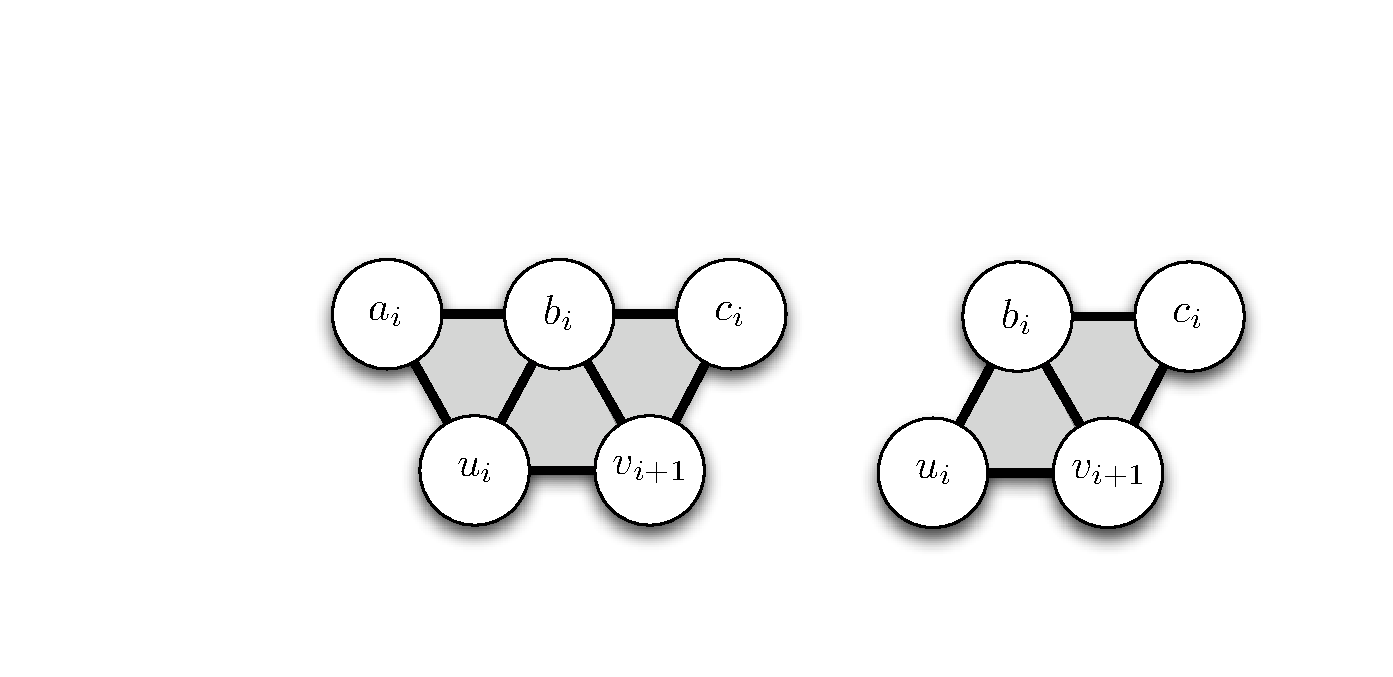
\includegraphics[width=3in]{./csa-32-22.pdf}
\end{center}
\fcaption{The carry-save adder (CSA), or 3-2 adder, and carry-save 2-2 adder.}
\label{fig:csa-3-2}
\end{figure}

At the level of numbers, the sum of three $n$-bit numbers can be converted into
the sum of two $n$-bit numbers by applying a \emph{CSA layer} of
$n$ parallel, single-bit
CSA circuits (Fig.~\ref{fig:csa-circuit}). Since each CSA operates in constant depth, the entire layer also
operates in constant depth, and we have achieved (non-modular) addition.
%
%An important consideration is the circuit width. The circuit above
%requires two additional qubits to contain the output
%out-of-place and produces two garbage qubits: the original inputs
%$b_i$ and $c_i$. 
Each single addition of three $n$-bit numbers requires $O(n)$ circuit width.

\section{Quantum Modular Addition}
\label{sec:csa-mod-add}

To perform addition of two numbers $a$ and $b$ modulo $m$,
we consider the variant problem of modular addition of three numbers to
two numbers:
%
%\begin{quote}
Given three $n$-bit input numbers $a$, $b$, and $c$, and an $n$-bit modulus $m$,
compute
%\begin{equation}
$(u+v) = (a+b+c)[m]$,
%\end{equation}
where $(u+v)$ is a CSE number.

In this section, we provide an alternate, pedagogical explanation of
Gossett's modular reduction \cite{Gossett1998}. Later, we contribute a mapping of this adder
to a 2D architecture,
using unbounded fanout to maintain constant depth for adding back
modular residues. This last step is absent in Gossett's original approach.

To start, we will demonstrate the basic method of modular addition and reduction
on an $n$-bit conventional number. In general, adding two $n$-bit conventional
numbers will produce an overflow bit of significance $2^n$, which we can truncate as long as
we add back its modular residue $2^n \bmod m$. How can we guarantee that we won't
generate another overflow bit by adding back the modular residue? It turns out
we can accomplish this by allowing
a slightly larger input and output number ($n+1$ bits in this case), truncating
multiple overflow bits, and adding back their $n$-bit modular residues.

For two $(n+1)$-bit conventional numbers $x$ and $y$,
we truncate the three high-order bits of their sum $z_{n-1,n+3}$
and
add back their modular residue $x_{(n-1,n)}[m]$:
%
\begin{eqnarray}
x + y \bmod m &=& z_{(0,n+1)}[m] \nonumber \\
&=& z_{(0,n-2)} + z_{(n-1,n+1)}[m].
\end{eqnarray}
%
Since both the truncated number $z_{(0,n-2)}$ and the modular residue
are $n$-bit numbers, their sum is an $(n+1)$-bit number as desired, equivalent
to $x[m]$.

Now we must do the same modular reduction on a CSE number $(u+v)$,
which in this case represents an $(n+2)$-bit conventional number and has
$2n+3$ bits.
%This is the special case mentioned in the
%previous
%section \label{star:csa-special}, where $x$ is the result of a single
%CSA layer, not repeated CSA layers alternating with truncation.
%
%Assume for now that this modular reduction works;
%in the next section we walk through an illustrated concrete example.
%We present a more formal argument in Section \ref{subsec:mod-reduce-1}.
%
First, we truncate the three high-order bits ($v_{n}, u_{n-1}, v_{n-1}$)
of $(u+v)$, yielding an $n$-bit
conventional number with a CSE representation of $2n$ bits:
$\{u_0, u_1, \ldots, u_{n-1}\} \cup \{v_1, v_2, \ldots, v_{n-1}\}$.
Then we add back the three modular residues
$(v_{(n+1)}[m], u_{(n)}[m], v_{(n)}[m])$, and we are guaranteed not to
generate additional overflow bits (of significance $2^{n}$ or higher). This equivalence
is shown in Equation \ref{eqn:mod-reduce}.
\begin{eqnarray}
(u+v)[m] &=& \left(u_{(0,n+1)} + v_{(1,n+2)}\right)[m] \nonumber \\
 &=& u_{(0,n)} +
     v_{(1,n)} + \nonumber \\
 & & u_{(n+1)}[m] +
     v_{(n+1)}[m] + v_{(n+2)}[m]
\label{eqn:mod-reduce}
\end{eqnarray}

\begin{lemma}[Modular Reduction in Constant Depth]
The modular addition of three $n$-bit numbers to two $n$-bit numbers can be
accomplished
in constant depth with $O(n)$ width in \textsc{2D CCNTC}.
\end{lemma}

\begin{proof}
Our goal is to show how to perform modular addition while keeping our numbers
of a fixed size by treating overflow bits correctly.
We map the proof of \cite{Gossett1998} to \textsc{2D CCNTC} and show that
we meet our required depth and width.
First, we enlarge our registers to allow the addition of $(n+2)$-bit numbers,
while keeping our modulus of size $n$ bits.
(In Gossett's original approach, he takes the equivalent step of restricting
the modulus to be of size $(n-2)$ bits.) We accomplish the modular addition
by first performing a layer of non-modular addition, truncating the three high-order
overflow bits, and then adding back modular residues controlled on these
bits in three successive layers, where we are guaranteed that no additional
overflow bits are generated in each layer.
This is illustrated for a $3$-bit modulus and $5$-bit registers
in Figure \ref{fig:csa-proof}.

\begin{center}
\begin{figure*}[h!tb]
\begin{displaymath}
\renewcommand\arraystretch{1.5}
\begin{array}{ccccccll}
        & a_4 & a_3 & a_2 & a_1 & a_0 & 5\text{-bit input number } a &\\
        & b_4 & b_3 & b_2 & b_1 & b_0 & 5\text{-bit input number } b & \\
        & c_4 & c_3 & c_2 & c_1 & c_0 & 5\text{-bit input number } c & \text{[Layer 1]}\\
\hline
        & u_4 & u_3 & u_2 & u_1 & u_0 & \text{truncate } u_{4} & \\
    v_5 & v_4 & v_3 & v_2 & v_1 &     & \text{truncate } v_{4},v_{5} & \\
        &     &     & c^{v_4}_2 & c^{v_4}_1 & c^{v_4}_0 & \text{add back } 2^4 \bmod m \text{ controlled on } v_4 & \text{[Layer 2]}\\
\hline
        &      & u'_3 & u'_2 & u'_1 & u'_0 & & \\
        & v'_4 & v'_3 & v'_2 & v'_1 &      & & \\
        &      &    & c^{u_4}_2 & c^{u_4}_1 & c^{u_4}_0  & \text{add back } 2^4 \bmod m \text{ controlled on } u_4 & \text{[Layer 3]}\\
\hline
        & u''_4 & u''_3 & u''_2 & u''_1 & u''_0 & \text{the bit } u''_4 \text{ is the same as } v'_4 & \\
        & v''_4 & v''_3 & v''_2 & v''_1 &       &  & \\
        &       &    & c^{v_5}_2 & c^{v_5}_1 & c^{v_5}_0 & \text{add back } 2^5 \bmod m \text{ controlled on } v_5 & \text{[Layer 4]}\\
\hline
        & u'''_4 & u'''_3 & u'''_2 & u'''_1 & u'''_0 & \text{ Final CSE output with } 5 \text{ bits} &\\
        & v'''_4 & v'''_3 & v'''_2 & v'''_1 &        & \text{ Final CSE output with } 5 \text{ bits} & \\
\end{array}
%\begin{array}{cccccccr}
%        & a_{n+1} & a_{n} & a_{n-1} & \ldots & a_1 & a_0 & \text{input number } a\\
%        & b_{n+1} & b_{n} & b_{n-1} & \ldots & b_1 & b_0 & \text{input number } b\\
%        & c_{n+1} & c_{n} & c_{n-1} & \ldots & c_1 & c_0 & \text{input number } c\\
%\hline
%        & u_{n+1} & u_{n} & u_{n-1} & \ldots & u_1 & u_0 & \text{truncate } u_{n+1} \\
%v_{n+2} & v_{n+1} & v_{n} & v_{n-1} & \ldots & v_1 & 0   & \text{truncate } v_{n+1},v_{n+2} \\
%        &         &       & x_{n-1} & \ldots & x_1 & x_0 \\
%\hline
%        &         & u'_{n} & u'_{n-1} & \ldots & u'_1 & u'_0 & \\
%        & v'_{n+1} & v'_{n} & v'_{n-1} & \ldots & v'_1 & 0 &  \\
%        &         &       & x_{n-1} & \ldots & x_1 & x_0 \\
%\hline
%        & u''_{n+1} & u''_{n} & u''_{n-1} & \ldots & u''_1 & u''_0 & \\
%        & v''_{n+1} & v''_{n} & v''_{n-1} & \ldots & v''_1 & 0 &  \\
%        &         &       & y_{n-1} & \ldots & y_1 & y_0 \\
%\hline
%        & u'''_{n+1} & u'''_{n} & u'''_{n-1} & \ldots & u'''_1 & u'''_0 & \\
%        & v'''_{n+1} & v'''_{n} & v'''_{n-1} & \ldots & v'''_1 & 0 &  \\
%\hline
%\end{array}
\end{displaymath}
\caption{A schematic proof of Gossett's constant-depth modular reduction for $n=3$.}
\label{fig:csa-proof}
\end{figure*}
\end{center}

We use the following notation.
The non-modular sum of the first layer is $u$ and $v$.
The CSE output of the first modular reduction layer
is $u'$ and $v'$, and the modular residue is
written as $c^{v_{n+1}}$ to mean the precomputed value $2^{n+1} \bmod m$
controlled on $v_{n+1}$.
The CSE output of the second modular reduction layer
is $u''$ and $v''$, and the modular residue is written as
$c^{u_{n+1}}$ to mean the precomputed value $2^{n+1} \bmod m$
controlled on $u_{n+1}$.
The CSE output of the third and final modular reduction layer
is $u'''$ and $v'''$, and the modular residue is written as
$c^{v_{n+2}}$ to mean the precomputed value $2^{n+2} \bmod m$
controlled on $v_{n+2}$.

We show that no layer generates an overflow $(n+2)$-bit, namely in the
$v$ component of any CSE output. (The $u$ component will never exceed the
size of the input numbers.) First, we know that no $v'_{n+2}$ bit
is generated after the first modular reduction layer, because we have
truncated away all $(n+1)$-bits. Second, we know that no $v''_{n+2}$ bit is
generated because we only have one $(n+1)$-bit to add, $v'_{n+1}$.
Finally, we need to show that $v'''_{n+2} = 0$ in the third modular reduction
layer. 

Since $u'_{(n)} + v'_{(n+1)} =
u_{(n)} + v_{(n)} \le 2^{n+1}$, the bits $u'_n$ and $v'_{n+1}$ cannot both be $1$.
But $u''_{n+1} = v'_{n+1}$ and $v''_{n+1} = u'_n\land v'_n$, so $u''_{n+1}$ and
$v''_{n+1}$ cannot both be $1$, and hence $v'''_{n+2} = 0$.
%This bit is the majority of
%$u''_{n+1}$, $v''_{n+1}$, and $c^{v_{n+2}}_{n+1} = 0$. This means we only have
%to guarantee that at most one of $u''_{n+1}$ and $v''_{n+1}$ has value 1.
%This is equivalent to requiring that
%$u''_{(n,n+1)} + v''_{(n+1)} \le 3\cdot 2^{n}$, that is, the sum of these
%three bits has value at most $3$. Bit $u''_{n+1}$ is copied directly from
%$v'_{n+1}$ by the rules of CSA, which requires the following condition for
%the second modular reduction layer:
%$u'_{(n)} + v'_{(n,n+1)} \le 3\cdot 2^n$. This is true because
%$u'_{(n)} + v'_{(n+1)} = u_{(n)} + v_{(n)} \le 2$ and $v'_{(n)} \le 1$.
Everywhere
we use the fact that the modular residues are restricted to $n$ bits.
Therefore, the modular sum is computed as the sum of two $(n+2)$-bit numbers
with no overflows in constant-depth.
\end{proof}

As a side note, we can perform modular reduction in one layer instead of
three by decoding the three overflow bits into one of seven different
modular residues. This can also be done in constant depth, and in this case
we only need to enlarge all our registers to $(n+1)$ bits instead of $(n+2)$
as in the proof above. We omit the proof for brevity.

In the following two subsections, we give a concrete example to illustrate
the modular addition circuit as well as a numerical upper bound for the
general circuit resources.

%%%%%%%%%%%%%%%%%%%%%%%%%%%%%%%%%%%%%%%%%%%%%%%%%%%%%%%%%%%%%%%%%%%%%%%%%%%%%%%
\subsection{A Concrete Example of Modular Addition}
\label{subsec:concrete}

\begin{center}
\begin{figure*}[h!bt]
\centerline{
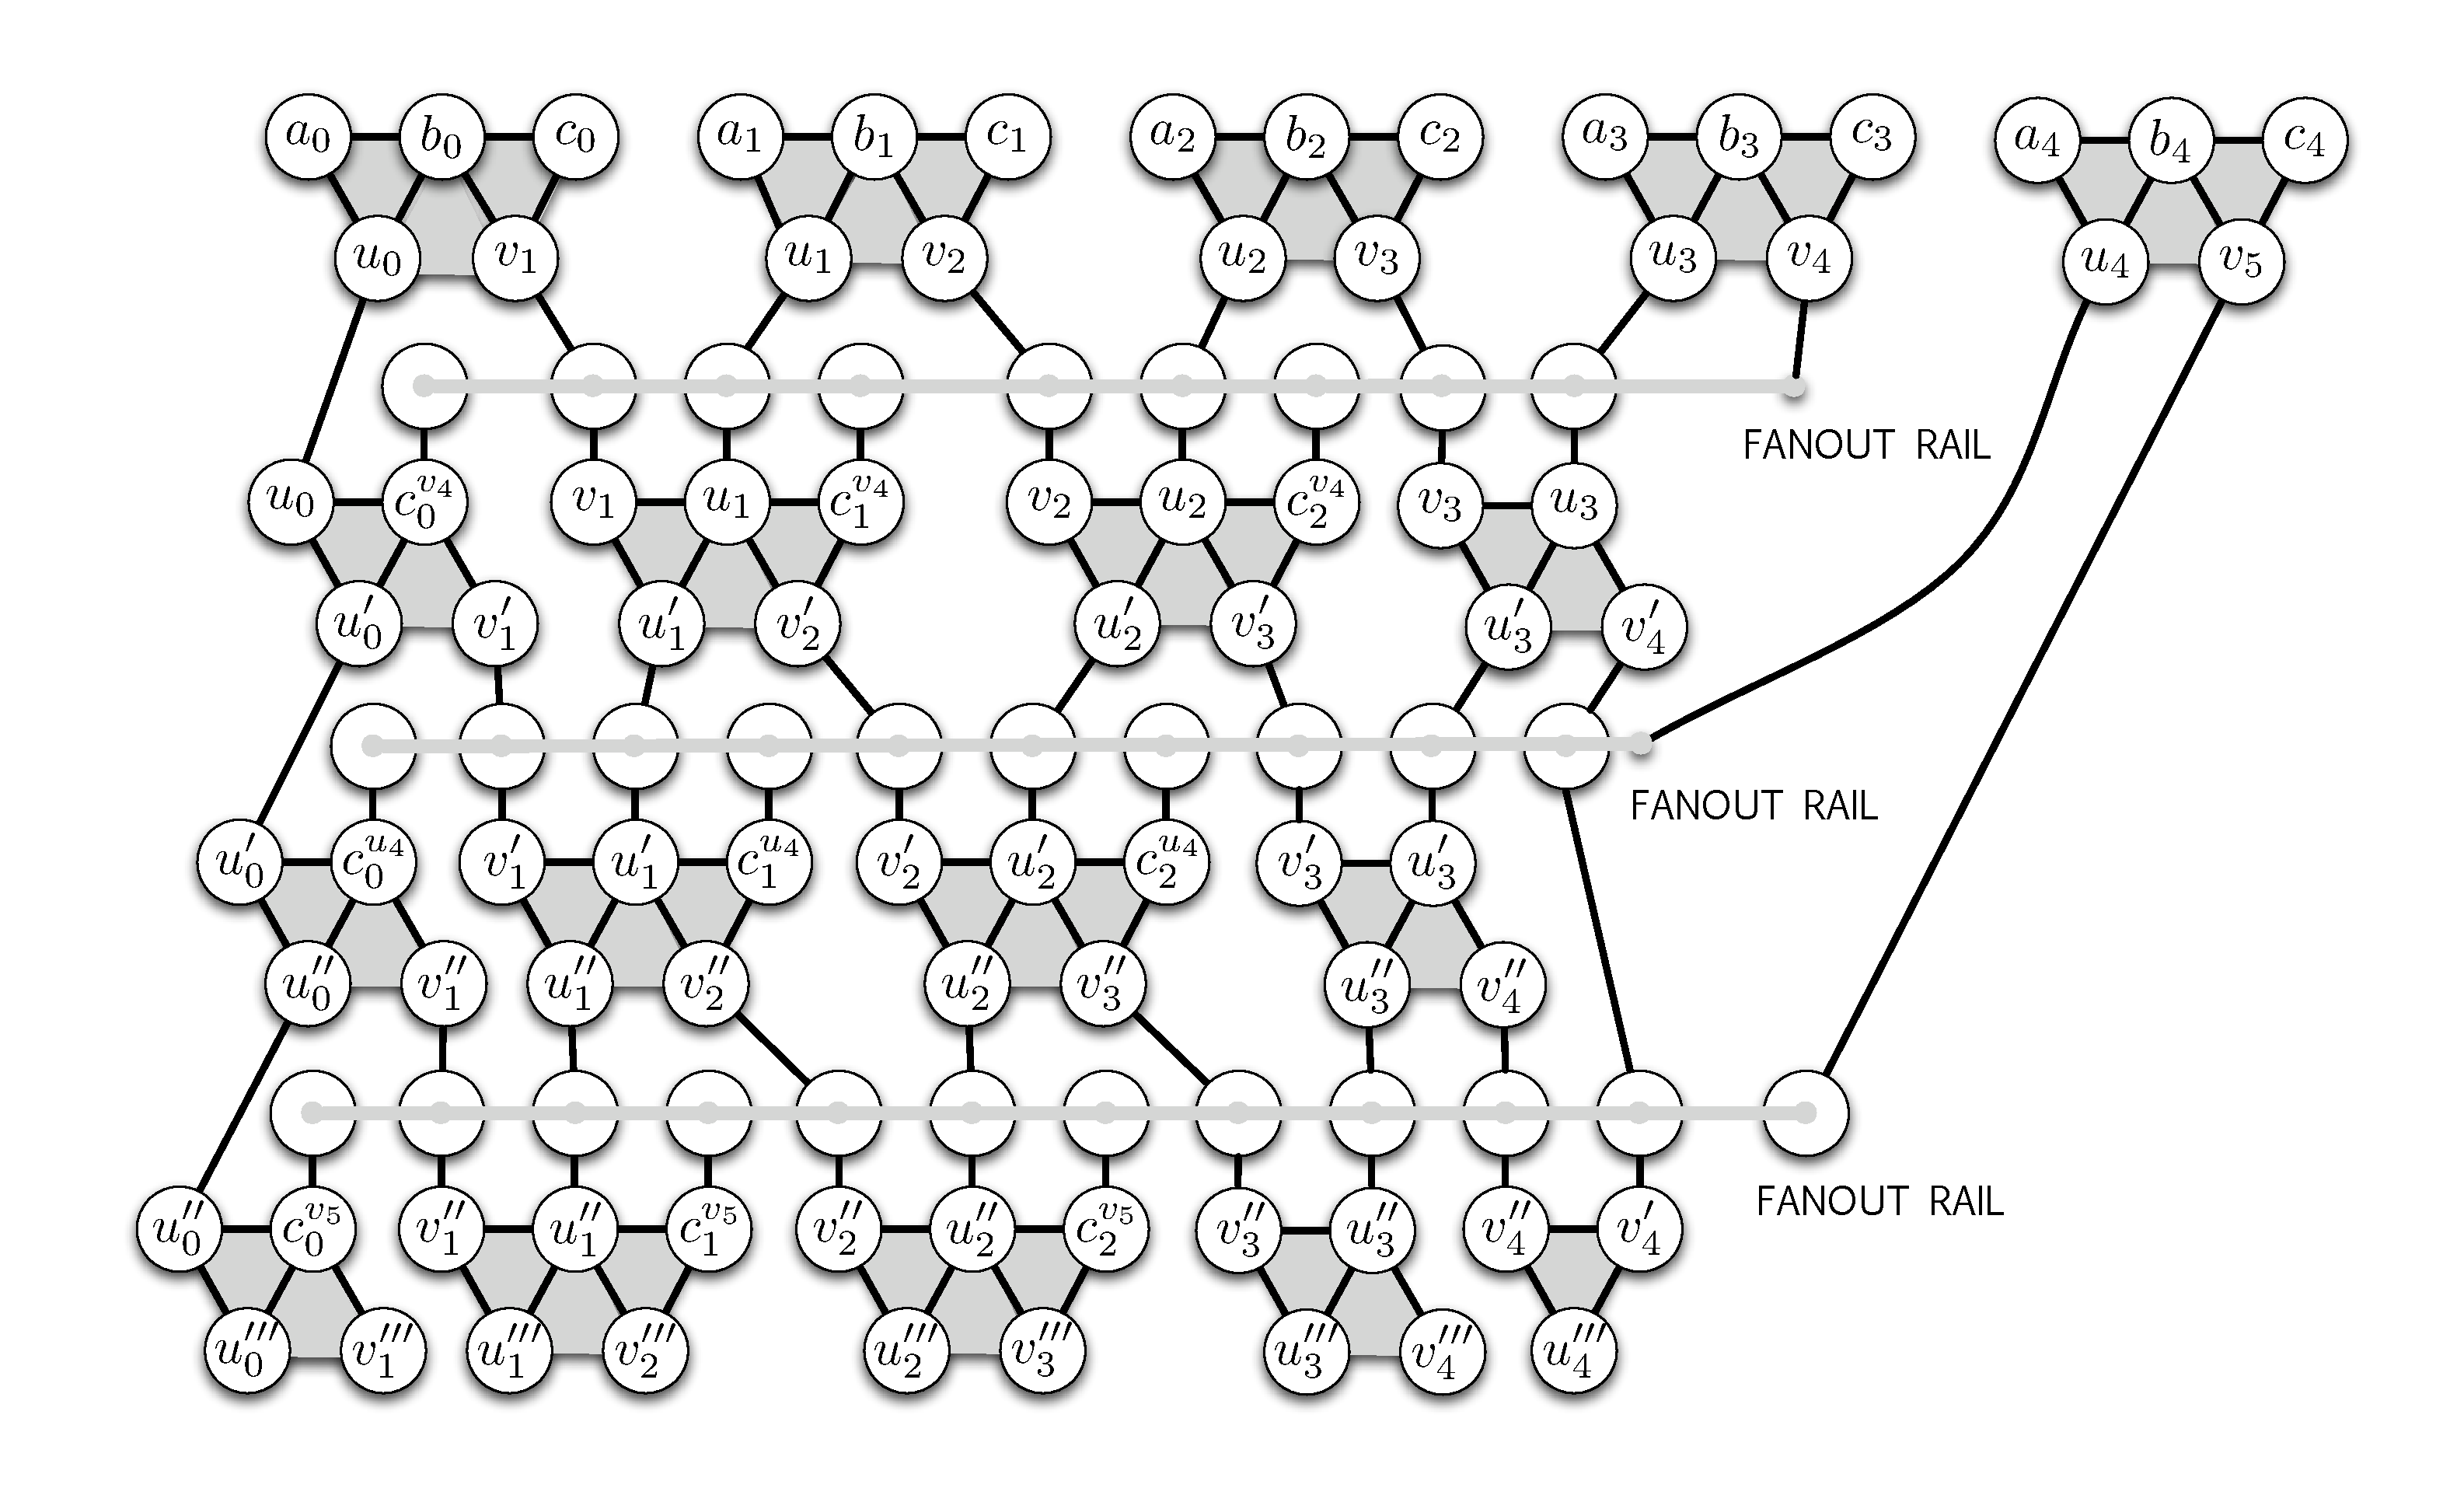
\includegraphics[width=6.5in]{factor-polylog/figures/mod-add-fixed.pdf}
}
\caption{Addition and three rounds of modular reduction for a 3-bit
modulus.}
\label{fig:csa-add-4}
\end{figure*}
\end{center}

A \textsc{2D CCNTC} circuit for modular addition of $5$-bit numbers using
four layers of parallel CSA's is shown graphically in Figure \ref{fig:csa-add-4}
which corresponds directly to the schematic proof in Figure \ref{fig:csa-proof}.
Note that in Figure \ref{fig:csa-add-4}, the least significant qubits are
on the left, and in Figure \ref{fig:csa-proof}, the least significant qubits are
on the right.
Figure \ref{fig:csa-add-4} also represents the approximate
physical layout of the qubits as they would look if this
circuit were to be fabricated.
Here, we convert the sum of three
$5$-bit integers into the modular sum of two $5$-bit integers, with a
$3$-bit modulus $m$.
In the first layer,
we perform 4 CSA's in parallel on the input numbers ($a,b,c$) and produce the
output numbers ($u, v$).

As described above, we truncate
the three high-order bits during the initial CSA round
(bits $u_4, v_4, v_5$) to retain a $4$-bit number.
Each of these bits serves as a control for adding its modular residue to
a running total. We can classically precompute $2^4[m]$ for the two
additions controlled on $u_4$ and $v_4$ and
$2^5[m]$ for the addition controlled on $v_5$.

In Layer 2,
we use a constant-depth fanout rail (see Figure \ref{fig:cdf}) to
distribute the control bit $v_4$ to its modular residue, which we denote as
%%\begin{equation}
$\ket{c^{v_4}} \equiv \ket{2^4[m]\cdot v_4}$.
%%\end{equation}
%This fanout requires constant depth;
The register $c^{v_4}$ has $n$ bits, which we add to the CSE results of layer 1.
The results $u_i$ and $v_{i+1}$ are teleported into layer 3. The exception is
$v'_4$ which is teleported into layer 4, since there are no other $4$-bits
to which it can be added. Wherever there are only
two bits of the same significance, we use the 2-2 adder from
Section \ref{sec:csa}.

Layer 3
%%, shown in Figure \ref{fig:csa-add-3},
operates similarly to layer 2, except that the modular residue is controlled on
$u_4$:
%%\begin{equation}
$\ket{c^{u_4}} \equiv \ket{2^4[m] \cdot u_4}$.
%%\end{equation}
%This fanout again requires constant depth;
The register $c^{u_4}$ has $3$ bits, which we
add to the CSE results of layer 2, where $u'_i$ and $v'_{i+1}$ are teleported
forward into layer 4.

Layer 4
%%, shown in Figure \ref{fig:csa-add-4},
is similar to layers 2 and 3, with the modular residue controlled on $v_5$:
%%\begin{equation}
$\ket{c^{v_5}} \equiv \ket{2^5[m] \cdot v_5}$.
%%\end{equation}
%This fanout is constant depth;
The register $c^{v_5}$ has $3$ bits, which we
add to the CSE results of layer 3.
There is no overflow bit $v'''_5$, and no carry bit from $v''_4$ and $v'_4$
as argued in the proof of Lemma 1.
The final modular sum $(a+b+c)[m]$ is $u'''+v'''$.

The general circuit for adding three $n$-qubit quantum integers to
two $n$-qubit quantum integers is called a \emph{CSA tile}. Each CSA tile in our architecture 
corresponds to its own module, and it will be represented by the symbol in 
Figure \ref{fig:csa-tile-symbol} for the rest of this paper. We call this
an $n$-bit modular adder, even though it accepts $(n+2)$-bit inputs, because
the size of the modulus is still $n$ bits.

\begin{center}
\begin{figure*}[h!bt]
\centerline{
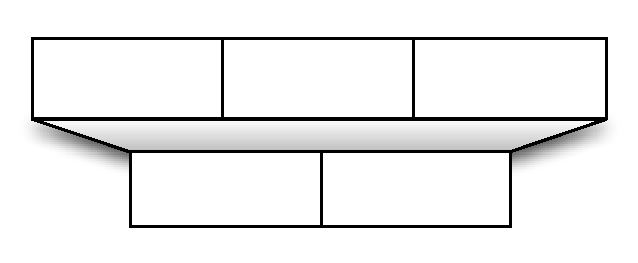
\includegraphics[width=1.5in]{factor-polylog/figures/csa-tile-symbol.pdf}
}
\caption{Symbol for an $n$-bit 3-to-2 modular adder, also called a CSA tile.}
\label{fig:csa-tile-symbol}
\end{figure*}
\end{center}


\subsection{Quantum Circuit Resources for Modular Addition}

We now calculate numerical upper bounds for the circuit resources of
the $n$-bit $3$-to-$2$ modular adder described in the previous section.
There are four layers of non-modular $n'$-bit $3$-to-$2$ adders, each of which
consists of $n'$ parallel single-bit adders whose
resources are detailed in Table \ref{tab:csa-tile-resources}. For factoring
an $n$-bit modulus, we have $n'=n+2$ in the first and fourth layers
and $n'=n+1$ in the second and third layers.

After each of the first three layers, we must move the output qubits
across the fanout rail to be the inputs of the next layer. We use
two swap gates, which have a depth and size of $6$ CNOTs each, since
the depth of teleportation is only more efficient for moving more than
two qubits. The control bit for each modular residue needs to be
teleported $0$, $4$, and $7$ qubits respectively according to the
diagram in Figure \ref{fig:csa-add-4}, before being fanned out $n$
times along the fanout rails, where the fanned out copies will end up
in the correct position to be added as inputs.

%The detailed resources for a Toffoli gate and the single-bit adder that uses
%them are given in Table \ref{tab:csa-tile-resources}.

The resources for the $n$-bit $3$-to-$2$ modular adder depicted in Figure
\ref{fig:csa-add-4} are given below.
The formulae reflect the resources needed for both computing the output
in the forward direction (including creating an entangled fanned-out state
controlled on overflow qubits)
and also uncomputing ancillae in the backward
direction (including disentangling previous fanned-out copies).

The circuit depth is $O(1)$:

\begin{equation}
374\text{.}
\end{equation}

The circuit size is $O(n)$:

\begin{equation}
551n + 757\text{.}
\end{equation}

The circuit width is $O(n)$:

\begin{equation}
33n + 47\text{.}
\end{equation}

\section{Quantum Modular Multiplication}
\label{sec:csa-mod-mult}

We can build upon our carry-save adder to implement quantum modular
multiplication in logarithmic depth. We start with a completely classical
problem to illustrate the principle of multiplication by repeated addition.
Then we consider modular multiplication of two quantum integers in a serial
and a parallel fashion in Section
\ref{subsec:csa-mod-mult-qq}. Both of these problems use as subroutines
\emph{partial product creation}, which we define and solve
 in Section \ref{subsec:ppc} and
 \emph{modular multiple addition}, which we define and solve
in Section \ref{subsec:mma}.

%%%%%%%%%%%%%%%%%%%%%%%%%%%%%%%%%%%%%%%%%%%%%%%%%%%%%%%%%%%%%%%%%%%%%%%%%%%%%%%
First we consider a completely classical problem:
given three $n$-bit classical numbers $a$, $b$, and $m$,
compute $c = ab \bmod m$, where $c$ is allowed to be in CSE.

We only have to add shifted
multiples of $a$ to itself, ``controlled'' on the bits of $b$. There are
$n$ shifted multiples of $a$, let's call them $z^{(i)}$, one for every bit of $b$:
%%\begin{equation}
$z^{(i)} = 2^i a b_i \bmod m$.
%%\end{equation}
We can parallelize the addition of $n$ numbers in a logarithmic depth
binary tree to get a total depth of $O(\log n)$.

%%%%%%%%%%%%%%%%%%%%%%%%%%%%%%%%%%%%%%%%%%%%%%%%%%%%%%%%%%%%%%%%%%%%%%%%%%%%%%
\subsection{Modular Multiplication of Two Quantum Integers}
\label{subsec:csa-mod-mult-qq}

We now consider the problem of multiplying a classical number controlled
on a quantum bit with a
\emph{quantum integer}\footnote{In this paper, an $n$-qubit 
quantum integer is a
general superposition of up to $2^n$ classical integers. As a special case,
a classical number controlled on a single qubit is a superposition of
$2$ classical integers.},
which is a
quantum superposition of classical numbers:

\begin{quote}
Given an $n$-qubit quantum integer $\ket{x}$, a control qubit $\ket{p}$,
and two $n$-bit classical numbers $a$
and $m$,
compute $\ket{c} = \ket{xa[m]}$, where $c$ is allowed to be in CSE.
\end{quote}

This problem occurs naturally in modular exponentiation (described in
the next section) and can be considered \emph{serial multiplication},
in that $t$ quantum integers are multiplied in series to a single
quantum register. This is used in serial QPF as mentioned in
Section \ref{sec:related}.


We first create $n$ quantum integers $\ket{z^{(i)}}$,
which are shifted multiples of the classical number $a$ controlled on the bits
of $x$:
%\begin{equation}
$\ket{z^{(i)}} \equiv \ket{2^i a[m] \cdot x_i }$.
%\end{equation}
These are typically called \emph{partial products} in a classical multiplier.
How do we create these numbers, and what is the depth of the procedure?
First, note that $\ket{2^i a[m]}$ is a classical number, so we can
precompute them classically and prepare them in parallel using single-qubit
operations
on $n$ registers, each consisting of $n$ ancillae qubits. Each $n$-qubit
register will hold a future $\ket{z^{(i)}}$ value.
We then fan out each of the
$n$ bits of $x$, $n$ times each, using an unbounded fanout operation so that
$n$ copies of each bit $\ket{x_i}$ are next to register $\ket{z^{(i)}}$.
This takes a total of $O(n^2)$ parallel CNOT operations.
We then entangle each $\ket{z^{(i)}}$ with the corresponding $x_i$.
%The schematic for this is shown in Figure \ref{fig:mod-mult-create}.
After this, we interleave these numbers into groups of three using
constant-depth teleportation. This reduces to the task of modular
multiple addition in order to add these numbers down to a single
(CSE) number modulo $m$, which is described in Section \ref{subsec:mma}.

%\begin{figure*}[htp!]
%\centerline{
%\includegraphics[width=4.5in]{./znumbers.pdf}
%}
%\caption{Creating $n=4$ shifted values $\{z^{(0)},z^{(1)},z^{(2)},z^{(3)}\}$
%for an input number $x$.}
%\label{fig:mod-mult-create}
%\end{figure*}

Finally, we tackle the most interesting problem:
\begin{quote}
Given two $n$-qubit quantum integers $\ket{x}$ and
$\ket{y}$ and an $n$-bit classical number
$m$,
compute $\ket{c} = \ket{xy \bmod m}$,
where $\ket{c}$ is allowed to be in CSE.
\end{quote}

This can be considered \emph{parallel multiplication} and is responsible
for our logarithmic speedup in modular exponentiation and parallel QPF.


Instead of creating $n$ quantum integers $\ket{z^{(i)}}$, we must create
up to $n^2$ numbers
$\ket{z^{i,j}}$ for all possible pairs of quantum bits $x_i$ and $y_j$,
$i,j \in \{0,\ldots,n-1\}$:
%\begin{equation}
$\ket{z^{i,j}} \equiv \ket{2^i2^j[m]\cdot x_i \cdot y_j}$.
%\end{equation}
We create these numbers using a similar procedure to the previous problem.
Adding $n^2$ quantum integers of $n$ qubits each takes depth
$O(\log(n^2))$, which is still $O(\log n)$.
Creating $n^2\times n$-bit quantum integers takes width $O(n^3)$.
Numerical constants are given for these resource estimates in
Section \ref{subsec:mod-mult-resources} for the entire modular multiplier.

Here is an outline of our modular multiplier construction, combining the
two halves of partial product creation (Section \ref{subsec:ppc}) and
modular multiple addition (Section \ref{subsec:mma}).

\begin{enumerate}
\item Initially, the inputs consist of the CSE quantum integers $x$ and $y$,
each with $2n+3$ bits, sitting on adjacent edges of a square lattice that has
sides of length $3(2n+3)$ qubits.
\item For each of $\lceil \log_2 (2n+3) \rceil$ rounds:
\begin{enumerate}
\item Of the existing $\{x_i\}$ and $\{y_j\}$ bits, apply a CNOT to create an
entangled copy in an adjacent qubit.
\item Teleport this new copy halfway between its current location and the
new copy.
\item At every site where an $\ket{x_i}$ and an $\ket{y_j}$ meet,
apply a Toffoli gate to create $\ket{x_i \cdot y_j}$.
\item Teleport $\ket{x_i \cdot y_j}$ to the correct $z$-site module.
\end{enumerate}
\item Within each $z$-site module, fanout $\ket{x_i \cdot y_j}$ up to $n$
times, corresponding to each $1$ in the modular residue $2^i 2^j \bmod m$,
to create the $n$-qubit quantum integer $\ket{z^{(i,j)}}$.
\item For each triplet of $z$-site modules, teleport the quantum integers
$\ket{z^{(i,j)}}$ to a CSA tile module, interleaving the three numbers so that
bits of the same significance are adjacent. This concludes partial product
creation (Section \ref{subsec:ppc}).
\item Perform modular multiple addition (described in Section \ref{subsec:mma})
on $t'$ $n$-qubit quantum integers down to 2 $n$-qubit quantum integers (one CSE number).
\item Uncompute all the previous steps to restore ancillae to $\ket{0}$.
\end{enumerate}
%%%%%%%%%%%%%%%%%%%%%%%%%%%%%%%%%%%%%%%%%%%%%%%%%%%%%%%%%%%%%%%%%%%%%%%%%%%%%%%
\subsection{Partial Product Creation}
\label{subsec:ppc}

This subroutine describes the procedure of creating $t'=O(n^2)$ partial products of
the CSE quantum integers $x$ and $y$, each with $2n+3$ bits each. We will now
discuss only the case of parallel multiplication. Although we
will not provide an explicit circuit for this subroutine, we will outline
our particular construction and give a numerical upper bound on the
resources required.

First, we need to generate the product bits
$\ket{x_i\cdot y_j}$ for all possible $(2n+3)^2$ pairs of $\ket{x_i}$ and
$\ket{y_j}$.
A particular product bit $\ket{x_i \cdot y_j}$
controls a particular classical number, the
$n$-bit modular residue $2^i 2^j [m]$, to form the partial product
$\ket{z^{(i,j)}}$ defined
in the previous section. However, some of these partial products
consist of only a single qubit, if $2^i 2^j < 2^n$, which is the minimum
value for an $n$-bit modulus $m$. There are at least $2n^2 - 2n + 1$
such single-bit partial products, which can be grouped into at most
$(2n+3)\times n$-bit numbers. Of the $(2n+3)^2$ possible partial products,
this leaves the number of remaining $n$-bit partial products as at most
$2n^2 + 14n +8$. Therefore we have a maximum number of $n$-bit
partial products, which we will simply refer to as $t'$ from now on.

\begin{equation}
t'=2n^2+16n+11
\label{eqn:tprime}
\end{equation}

The creation of the product bits $\ket{x_i \cdot y_j}$ occurs on a
square lattice of $(3(2n+3))^2$ qubits, with the numbers $\ket{x_i}$ and
$\ket{y_j}$ located on adjacent edges. The factor of $3$ in the size of the lattice
allows the $\ket{x_i}$ and $\ket{y_j}$ bits move past each other.
The $\ket{x_i}$ bits are teleported along an axis that is perpendicular to
the teleportation axis for the $\ket{y_j}$ bits, and vice versa.
Product bit creation, and this square lattice, comprise a single module.
In $\lceil \log_2 (2n+3) \rceil$
rounds, these bits are copied via a CNOT and teleported to the middle of
a recursively halved interval of the grid. The copied bits $\ket{x_i}$ and
$\ket{y_j}$
first form $1$ line, then $3$ lines, then $7$ lines, and so forth,
intersecting at $1$ site, then $9$ sites, then $49$ sites, and so forth.
There are $\lceil \log_2 (2n+3) \rceil$ such rounds.

At each intersection, a Toffoli gate is used to create $\ket{x_i \cdot y_j}$
from the given $\ket{x_i}$ and $\ket{y_j}$. These product bits are then
teleported away from this qubit, out of this product bit module, to different
modules where the $\ket{z^{(i,j)}}$ numbers are later generated,
called $z$-sites. There are $t'$ $z$-site modules which each contain 
an $n$-qubit quantum integer. Any
round of partial product generation will produce at most as many product
bits $x_i \cdot y_j$ as in the last round, which is half the total number
of $(2n+3)^2$.
%These product bits are teleported out the two sides of the
%square lattice that are opposite the input numbers $x$ and $y$, which means the
%square lattice has dimension at most $((2(2n+3)-1)(n+2))^2 = O(n^4)$.

%The $z$-sites have total width of $3nt'$ qubits, so the maximum total
%teleportation length of all qubits is $(2n+3)^2$ multiplied by the maximum
%length of any single teleportation length,
%Our construction consists of the following steps:

We now present the resources for partial product creation, the first half of
a modular multiplier, including the reverse computation.

The circuit depth is $O(\log n)$:

\begin{equation}
D_{PPC} = 32\log_2 n + 150\text{.}
\end{equation}

The module depth is $O(1)$:

\begin{equation}
\overline{D}_{PPC} = 8\text{.}
\end{equation}

The circuit size is $O(n\log^2 n)$:

\begin{eqnarray}
S_{PPC} & = & (6n + 9)\log_2 n +\\
        &   & (26n^3 + 232n^2 + 224n + 159)\text{.}
\end{eqnarray}

The module size is $O(n^2)$:

\begin{eqnarray}
\overline{S}_{PPC} = 6n^2 + 26n + 19\text{.}
\end{eqnarray}

The circuit width is $O(n^3)$:

\begin{eqnarray}
W_{PPC} = 6n^3 + 48n^2 - 8n + 1\text{.}
\end{eqnarray}

The module width is $O(n^2)$:

\begin{eqnarray}
\overline{W}_{PPC} = 2n^2 + 14n + 9\text{.}
\end{eqnarray}

%%%%%%%%%%%%%%%%%%%%%%%%%%%%%%%%%%%%%%%%%%%%%%%%%%%%%%%%%%%%%%%%%%%%%%%%%%%%%%%
\subsection{Modular Multiple Addition}
\label{subsec:mma}

As a subroutine to modular multiplication, we define the operation of
repeatedly adding multiple numbers down to a single CSE number, called
\emph{modular multiple addition}.

The modular multiple addition circuit generically adds down $t'\times n$-bit
conventional numbers to an $n$-bit CSE number:
%
\begin{equation}
z^{(1)} + z^{(2)} + \ldots z^{(t')} \equiv (u+v)[m].
\end{equation}
%
It does not matter how the
$t'$ numbers are generated, as long as they are divided into groups of three
and have their bits interleaved to be the inputs of a CSA tile.
From the previous section, serial multiplication results in
$t' \le n$ and parallel multiplication results in $t' \le n^2$. Each CSA tile
is contained in its own module. These modules are arranged in layers within
a logarithmic depth binary tree, where 
the first layer contains $\lceil t'/3 \rceil$ modules. A modular addition
occurs in all the modules of the first layer in parallel. The outputs from this
first layer are then teleported to be the inputs of the next layer of modules,
which have at most two-thirds as many modules. This continues until the
tree terminates in a single module, whose output is a CSE number $u+v$ which
represents the modular product of all the original $t'$ numbers. The resulting
height of the tree is $(\lceil \log_{3/2}(t'/3) \rceil + 1)$ modules.

As the parallel modular additions proceed by layers, all previous layers
must be maintained in a coherent state, since the modular addition leaves
garbage bits behind. Only at the end of modular multiple addition, after
the final answer $u+v$ is obtained, can all the previous layers be
uncomputed in reverse to free up their ancillae.

These steps are best illustrated with a concrete
example in Figure \ref{fig:mod-mult}. The module for each CSA tile is
represented by the symbol from Figure \ref{fig:csa-tile-symbol}.
The arrows indicate the
teleportation of output numbers from the source tile to be input numbers
into a destination tile.

\begin{figure*}[htb!]
\centerline{
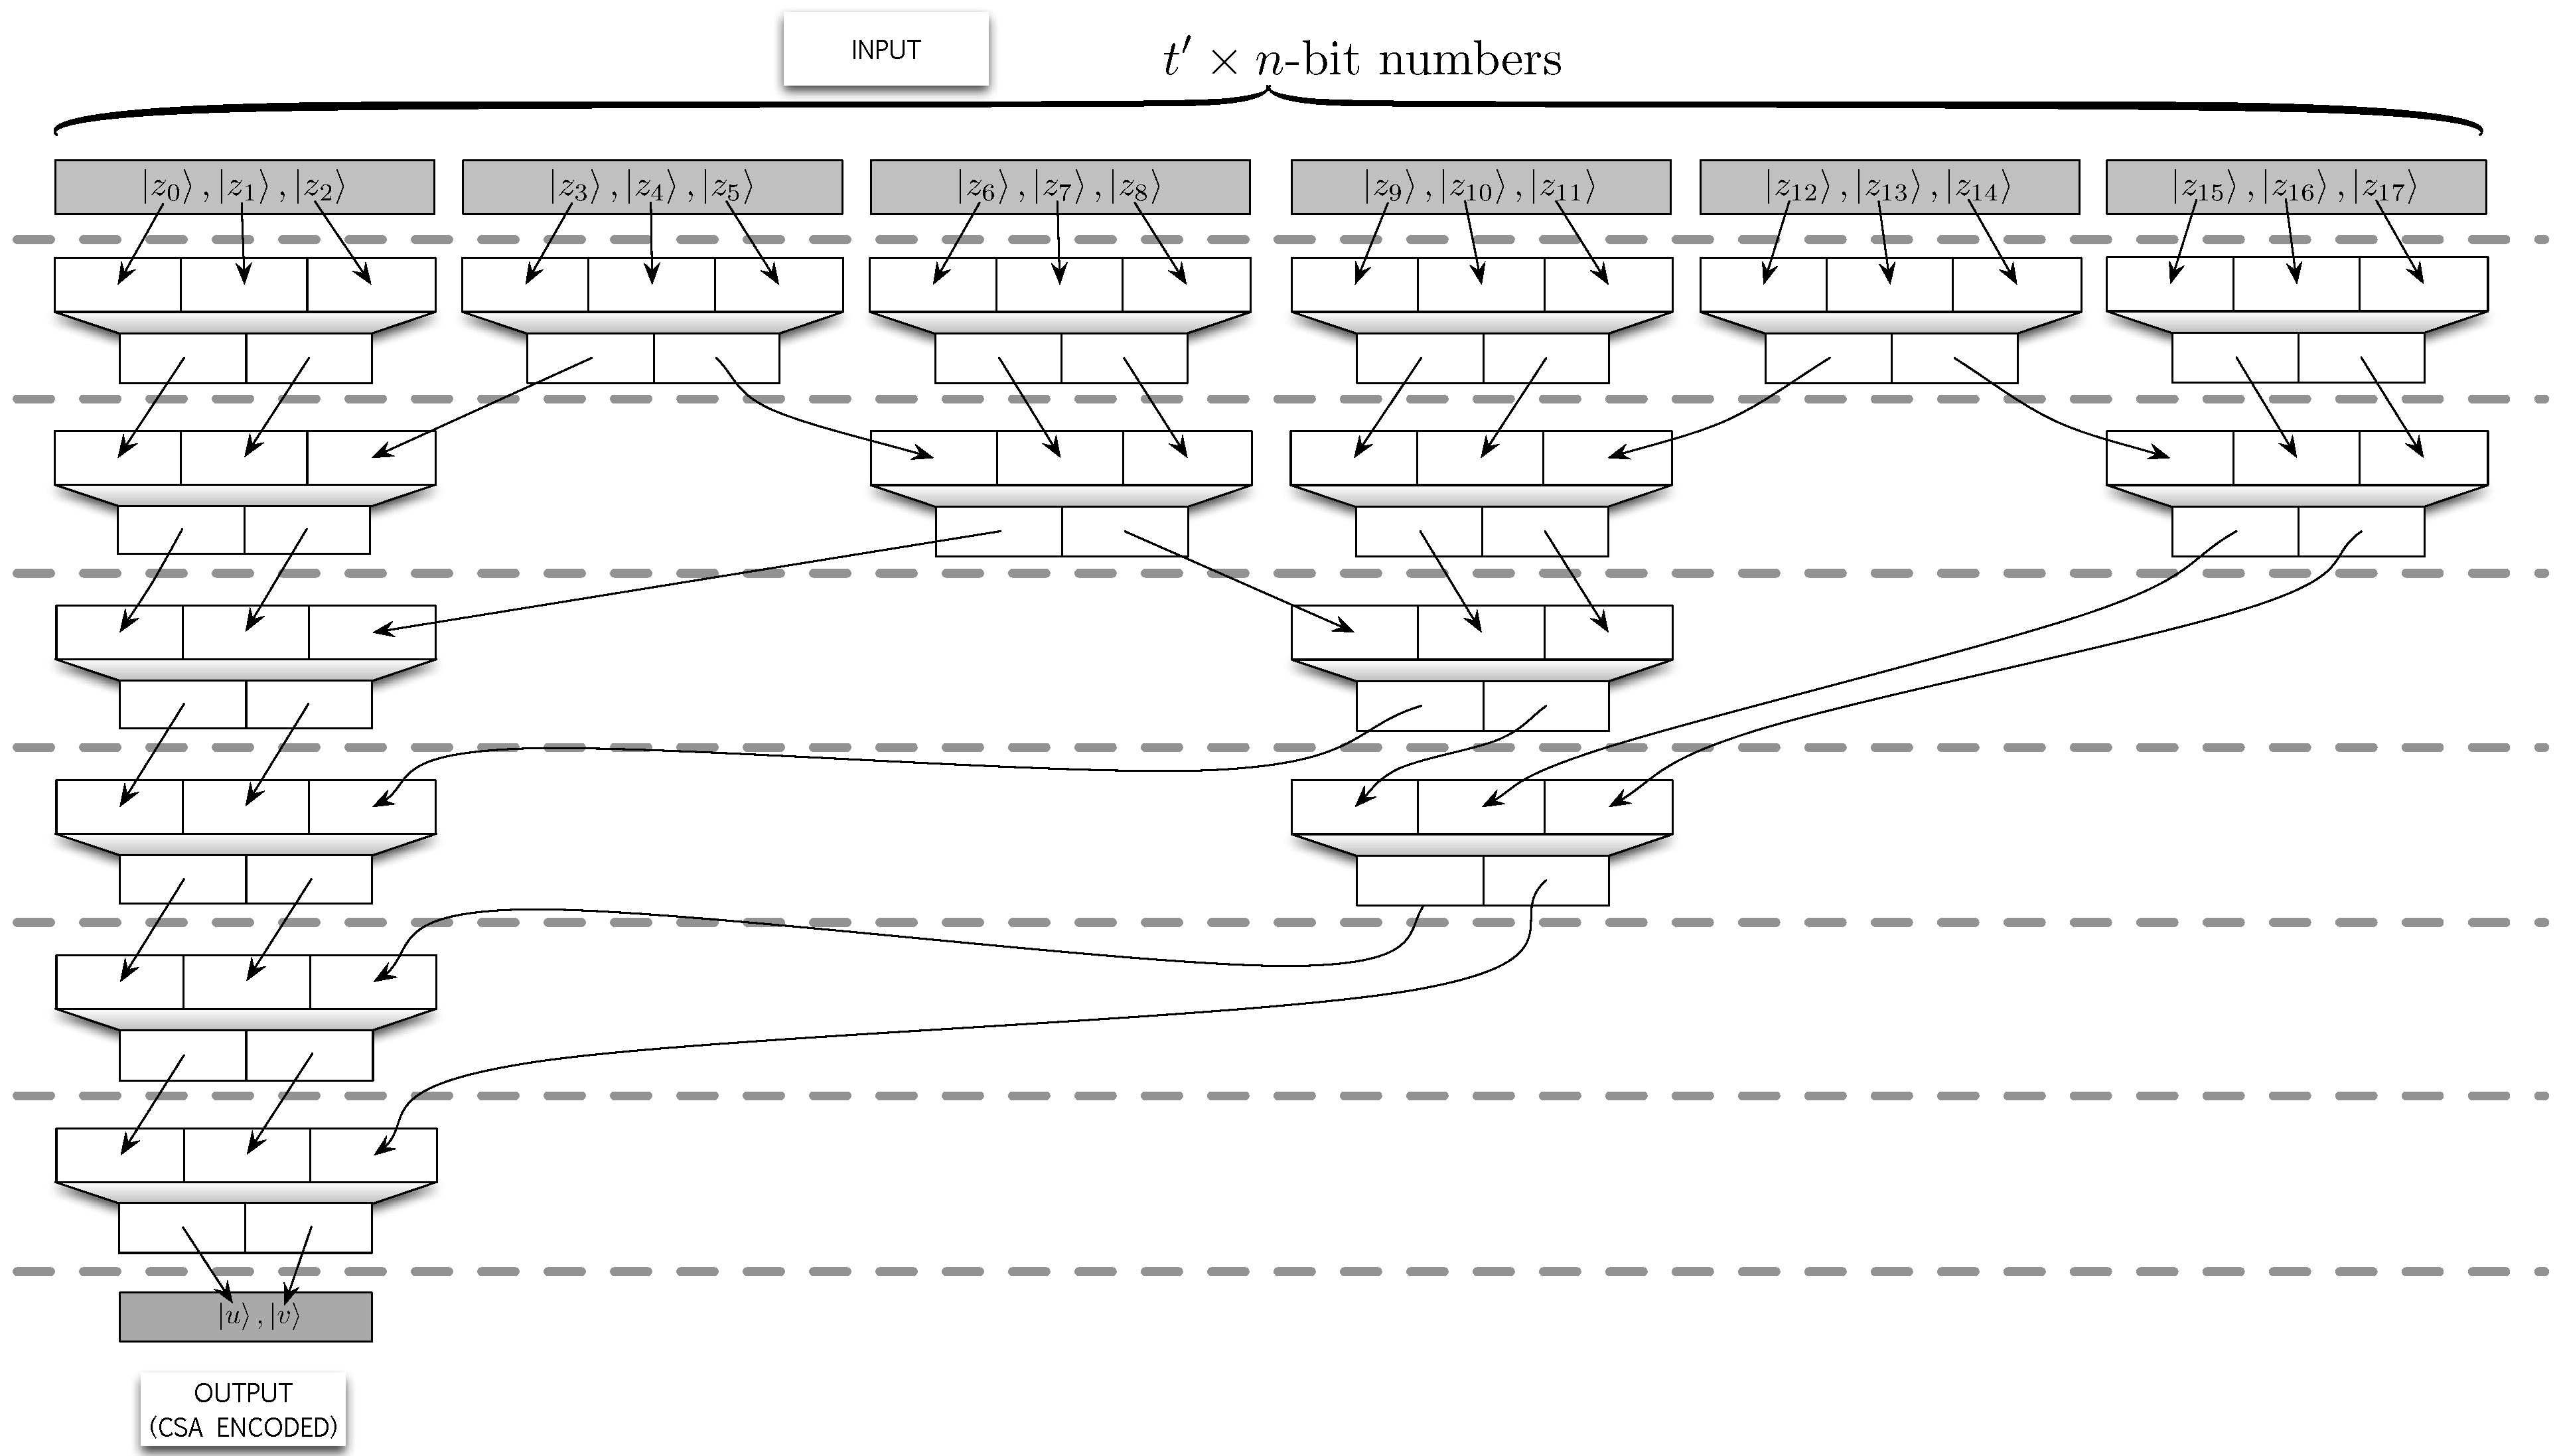
\includegraphics[width=5.5in]{factor-polylog/figures/mod-mult-add.pdf}
}
\caption{Modular multiple addition of quantum integers on a CSA tile
architecture for $t'=18$ in a logarithmic-depth tree with height $(\lceil \log_{\frac{3}{2}}(t'/3) \rceil + 1) = 6$. Arrows represent teleportation
in between modules.}
\label{fig:mod-mult}
\end{figure*}
%

Now we can analyze the circuit resources for multiplying $n$-bit
quantum integers, which requires $(t'-2)$ modular additions, for $t'$ from
Equation \ref{eqn:tprime}.
The circuit width is the sum of the $O(n^3)$ ancillae
needed for partial product creation and the ancillae required for $O(n^2)$
modular additions. Each modular addition has width $O(n)$ and depth $O(1)$
from the previous
section. There are
$\lceil \log_{3/2}(n^2 / 3) \rceil +1 $ timesteps of modular addition. Therefore
the entire modular multiplier circuit has depth $O(\log n)$ and width $O(n^3)$.

\subsection{Modular Multiplier Resources}
\label{subsec:mod-mult-resources}.

The circuit depth of the entire modular multiplier is $O(\log n)$:

\begin{equation}
D_{MM} = 1383 \log_2 n + 3930\text{.}
\end{equation}

The module depth is $O(\log n)$:
\begin{equation}
\overline{D}_{MM} = 2\log_2 n + 11\text{.}
\end{equation}

The circuit size is $O(n^3)$:

\begin{eqnarray}
S_{MM} = & (6n + 9)\log_2 n +\\
        & (1152n^3 + 10780n^2 + 17628n + 7082)\text{.}
\end{eqnarray}

The module size is $O(n^3)$:

\begin{equation}
\overline{S}_{MM} = 15n^3 + 127n^2 + 178n + 50{.}
\end{equation}

The circuit width is $O(n^3)$:

\begin{equation}
W_{MM} = 66n^3 + 558n^2 + 870n + 290\text{.}
\end{equation}

The module width is $O(n^2)$:

\begin{equation}
\overline{W}_{MM} = 4n^2 + 28n + 15\text{.}
\end{equation}

\section{Quantum Modular Exponentiation}
\label{sec:modexp}

We now extend our arithmetic to modular exponentiation, which is repeated
modular multiplication controlled on qubits supplied by a phase estimation
procedure.
If we wish to multiply an $n$-qubit quantum input number $\ket{x}$ by
$t$ classical numbers $a^{(j)}$, we can multiply them in series.
% as shown in
%Figure \ref{fig:modexp-qc-series}.
This requires depth $O(t\log n)$ in modular multiplication operations.

%\begin{figure}[htp!]
%\begin{center}
%\includegraphics[width=5.5in]{figures/modexp-qc-series.pdf}
%\end{center}
%\caption{Multiplying a quantum number $\ket{x}$ by $t$ classical numbers
%$\{a^{0}, a^{1}, \ldots, a^{n-1}\}$ in series.}
%\label{fig:modexp-qc-series}
%\end{figure}

Now consider the same procedure, but this time each classical number $a^{(j)}$
is controlled on a quantum bit $p_j$. This is a special case of
multiplying by $t$ quantum integers in series, since a classical number
entangled with a quantum integer is also quantum.
%This is shown in
%Figure \ref{fig:modexp-qq-series}.
It takes the same depth $O(t\log n)$ as the previous case.
%
%\begin{figure}[htp!]
%\begin{center}
%\includegraphics[width=5.5in]{figures/modexp-qq-series.pdf}
%\end{center}
%\caption{Multiplying a quantum number $\ket{x}$ by $t$ quantum numbers
%$\{\ket{a^{0}p_0}, \ket{a^{1}p_1}, \ldots, \ket{a^{n-1}p_{n-1}}\}$ in series.}
%\label{fig:modexp-qq-series}
%\end{figure}

Finally, we consider multiplying $t$ quantum integers
$\{x^{(1)}, x^{(2)}, \ldots, x^{(t-1)}, x^{(t)}\}$ in a parallel,
logarithmic-depth binary tree.
This is shown in Figure \ref{fig:modexp-qq-parallel}, where arrows indicate multiplication.
The tree has depth $\log_2(t)$ in modular multiplier operations. Furthermore,
each
modular multiplier has depth $O(\log(n))$ and width $O(n^3)$ for $n$-qubit
numbers. Therefore, the overall depth of this parallel modular exponentiation
structure is $O(\log(t)\log(n))$ with width $O(tn^3)$.
In phase estimation for QPF, it is
sufficient to take $t = O(n)$ \cite{Nielsen2000,Kitaev2002}. Therefore our total depth is
$O(\log^2(n))$ and our total size and total width are $O(n^4)$, as desired. At this point, combined with the parallel phase
estimation procedure of \cite{Kitaev2002}, we have a complete factoring
implementation in our hybrid 2D nearest-neighbor architecture in poly-logarithmic
depth.
%
\begin{figure*}[tb!]
\centerline{
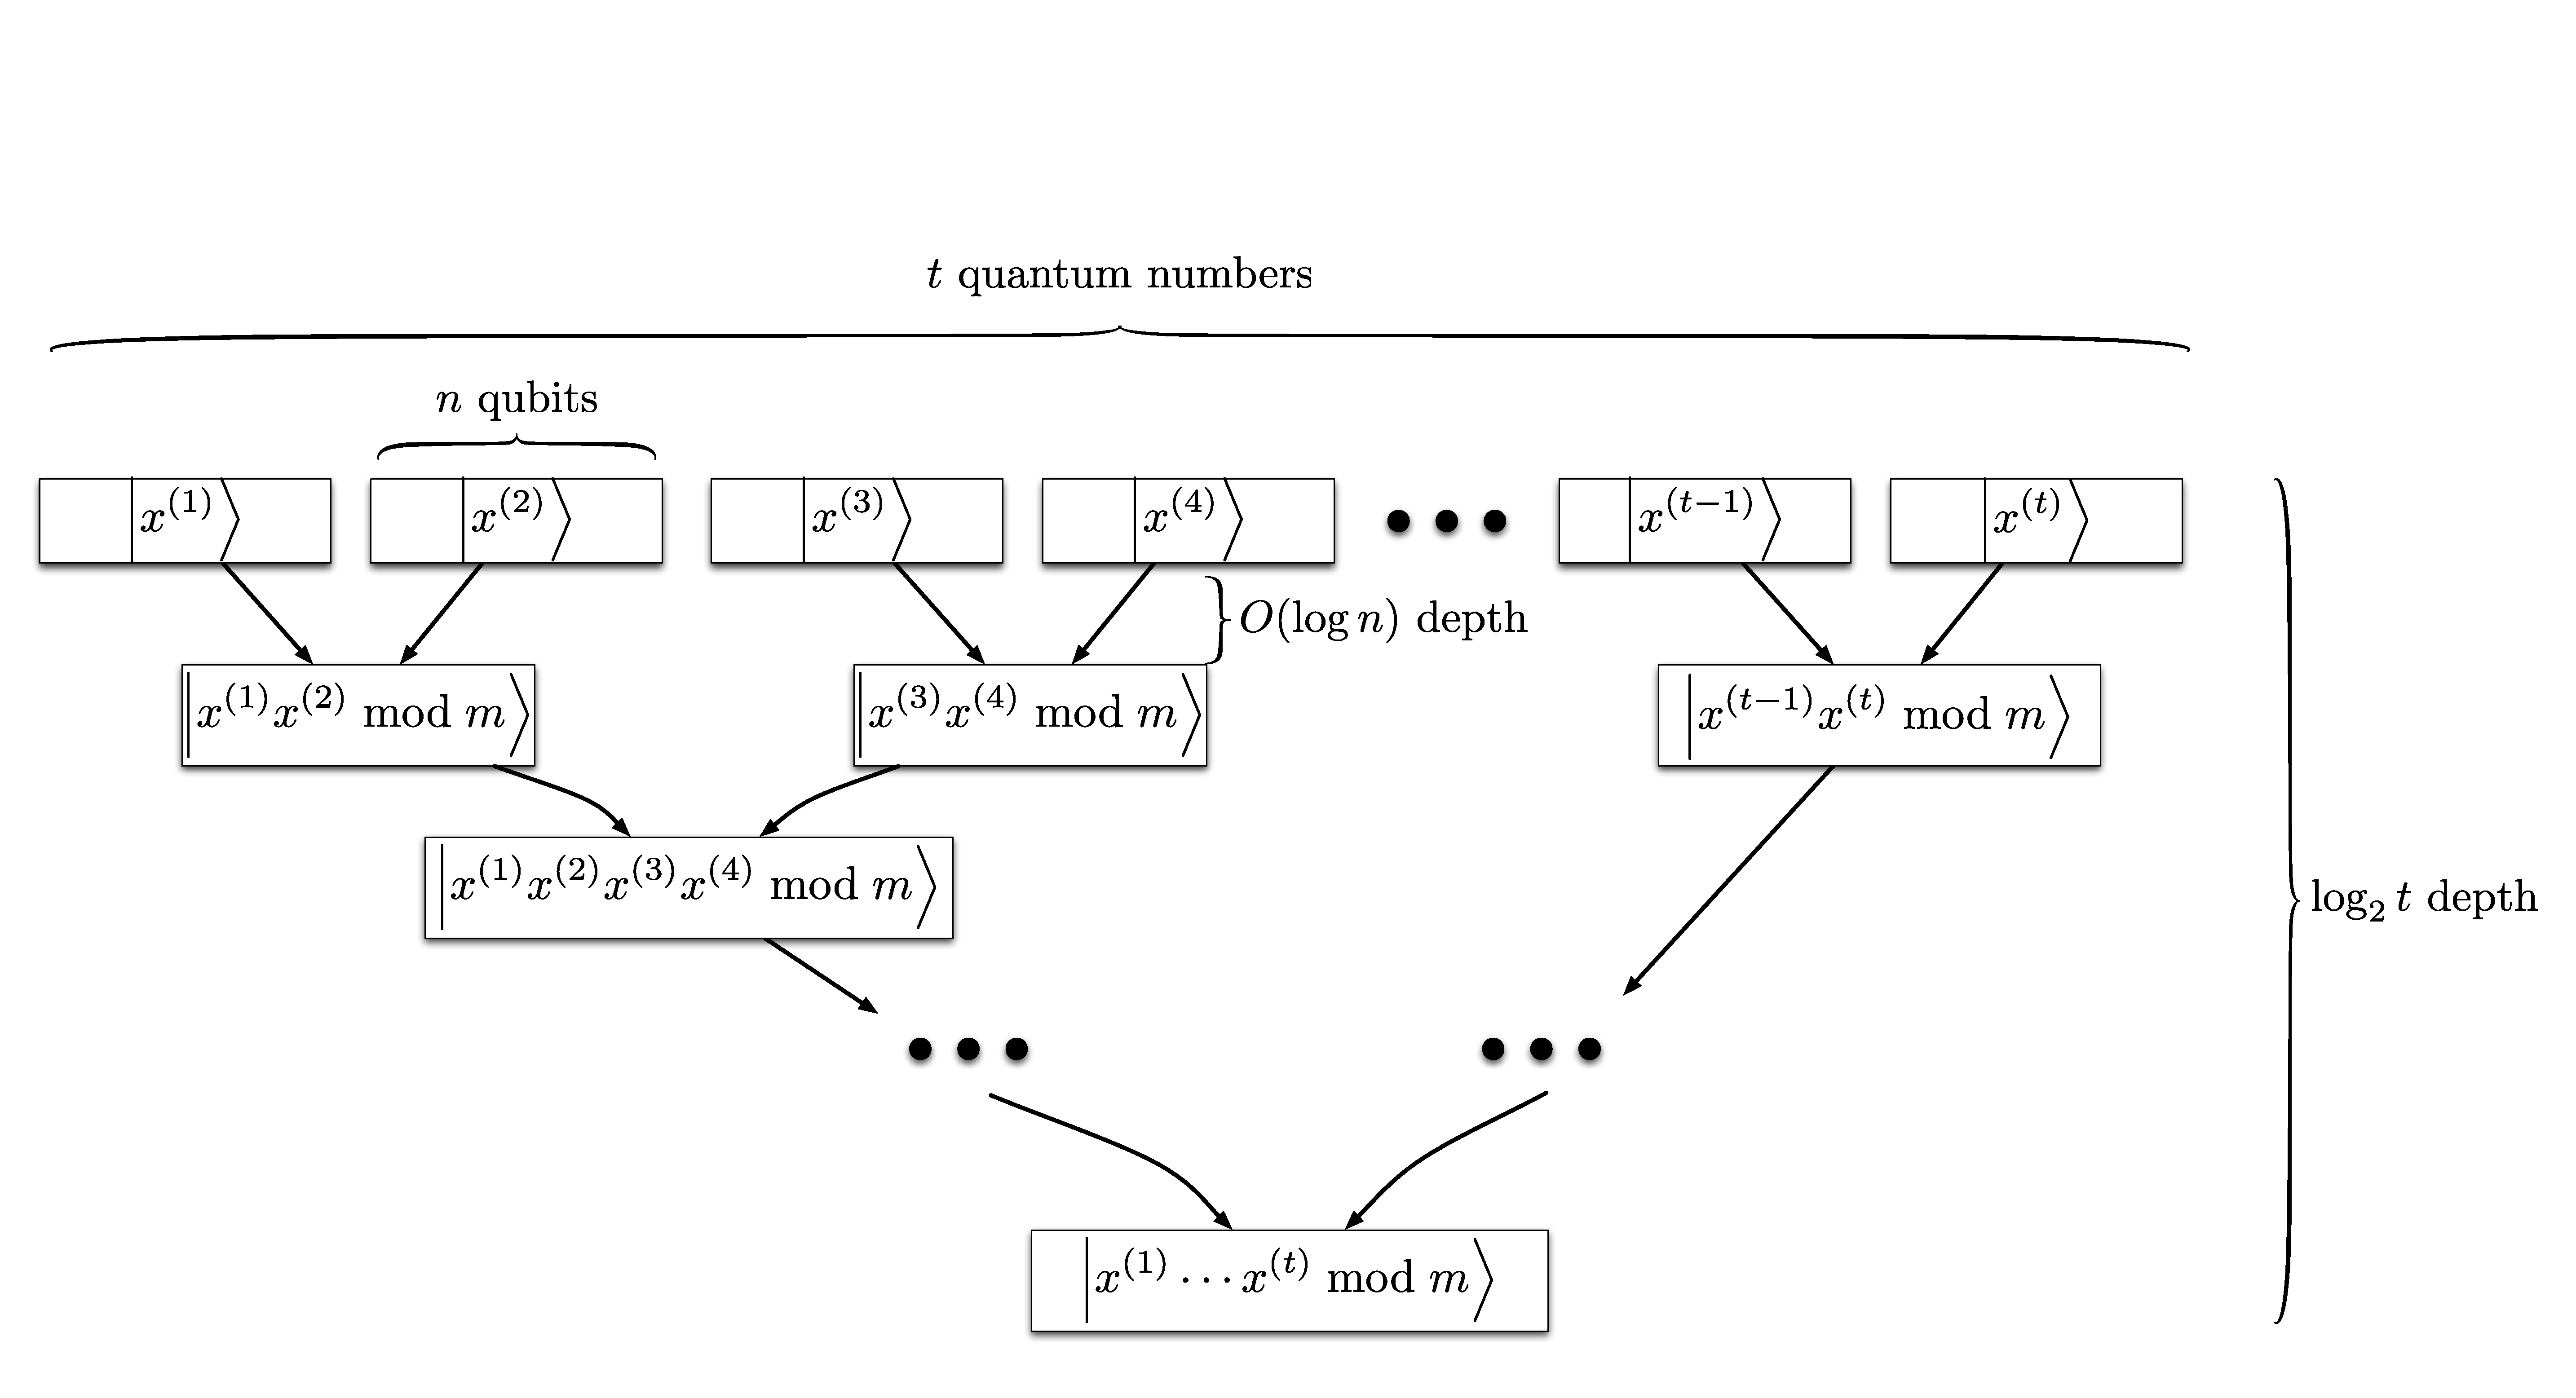
\includegraphics[width=5.5in]{factor-polylog/figures/mod-exp-par.pdf}
}
\caption[Parallel modular exponentiation]
{Parallel modular exponentiation: multiplying $t$ quantum integers
%$\{\ket{x^{(0)}}, \ket{x^{(1)}}, \ldots, \ket{x^{(t-1)}}\}$ in parallel,
in a $O(\log{(t)}\log{(n)})$-depth binary tree. Arrows indicate modular
multiplication.}
\label{fig:modexp-qq-parallel}
\end{figure*}

We will now calculate numerical
constants to upper bound circuit resources.

According to the Kitaev-Shen-Vyalyi parallelized phase estimation procedure
\cite{Kitaev2002},
for a constant success probability of $3/4$,
it is sufficient to multiply together $t = 2867n$ quantum integers,
controlled on the qubits $\ket{p_j}$, in parallel.

In Section \ref{subsec:qcla}, we describe the last step of modular
exponentiation in CSE. In Section \ref{subsec:modexp-resources}, we
state the final circuit resources for the entire modular exponentiation
circuit,
and therefore, our quantum period-finding procedure.

%%%%%%%%%%%%%%%%%%%%%%%%%%%%%%%%%%%%%%%%%%%%%%%%%%%%%%%%%%%%%%%%%%%%%%%%%%%%%%
\subsection{Converting Back to a Unique Conventional Number}
\label{subsec:qcla}

The final product of all $t$ quantum integers is in CSE which is not
unique. As stated in Gossett's original paper \cite{Gossett1998}, this
must be converted back to a conventional number using, for example, the
quantum carry-lookahead adder (QCLA) from \cite{Draper2004}. We can convert
this to a nearest-neighbor architecture by using the qubit reordering
construction of \cite{Rosenbaum2012}. We now compute the resources
needed for this last step.

To add two $(n+2)$-bit numbers in a QCLA, we have a circuit width of
$k = (4(n+2) - 2\log_2 n - 1)$. The depth is at most $4\log_2 n +2$ gates,
and some of them act on qubits that are not nearest-neighbors. Therefore,
we add in between each gate a reordering circuit that takes $k^2$
(reusable) ancillae
qubits and uses two rounds of constant-depth teleportation to rearrange
the qubits into a new order where all the gates are nearest-neighbor.
Adding in the teleportation circuit resources from Table \ref{tab:cd-resources},
we can calculate the following resources.

The circuit depth is $O(\log n)$:
%
\begin{equation}
D_{QCLA} = 56\log_2 n + 28\text{.}
\end{equation}
%
The circuit size is $O(n^2 \log n)$:
%
\begin{eqnarray}
S_{QCLA} = 96 \log_2^3 n & - & (384n + 624)\log_2^2 n \nonumber \\
              & + & (384n^2 + 1152n + 840) \log_2 n \nonumber \\
              & + & (192n^2 + 672n + 588)\text{.}
\end{eqnarray}
%
The circuit width is $O(n^2)$:
%
\begin{equation}
W_{QCLA} = 4 \log_2^2 n - (16n + 30)\log_2 n + 16n^2 + 60n + 56\text{.}
\end{equation}


%%%%%%%%%%%%%%%%%%%%%%%%%%%%%%%%%%%%%%%%%%%%%%%%%%%%%%%%%%%%%%%%%%%%%%%%%%%%%%
\subsection{Circuit Resources for Modular Exponentiator}
\label{subsec:modexp-resources}

This leads to the following circuit resource upper bounds for a modular exponentiator. Therefore, these are the total resources for running a
single round of parallel QPF as part of Shor's factoring algorithm.

The circuit depth is $O(\log^2 n)$:
% From Notebook #16 p. 225, N18, p. 3-4
\begin{equation}
D_{ME} = 1383\log_2^2(n) + 21253\log_2(n) + 49098\text{.}
\end{equation}
%
The module depth is $O(\log^2 n)$:
%
\begin{equation}
\overline{D}_{ME} = 3\log_2 n + 24
\end{equation}
%
The circuit size is $O(n^4)$:
%
\begin{eqnarray}
S_{ME} & = & 96 \log_2^3 n + \nonumber \\
       & - & (384n + 624)\log_2^2 n \nonumber \\
       & + & (384n^2 + 1152n + 840) \log_2 n \nonumber \\
       &   & 3302324 n^4 + 30900797 n^3 + 50527571 n^2  + 20287173 n + 
  -6494\text{.}
\label{eqn:sme}
\end{eqnarray}
%
The module size is $O(n^4)$:
%
\begin{eqnarray}
\overline{S}_{ME} & = & (17202 n^2 + 25797 n - 9) \log_2 n + \nonumber \\
                  & + & 3302784 n^4 + 30905108 n^3 50534430 n^2 + 20295063 n - 7088 \text{.}
\end{eqnarray}
%
The circuit width is $O(n^4)$:
%
\begin{equation}
W_{ME} = 94598n^4 + 799749 n^3 + 1246692 n^2 + 418089 n - 145\text{.}
\end{equation}
%
The module width is $O(n^3)$:
%
\begin{equation}
\overline{W}_{ME} = 5736 n^3 + 40152 n ^2 + 21510 n\text{.}
\end{equation}

\section{Asymptotic Results}
\label{sec:fpl-results}

The asymptotic resources required for our approach,
as well as the resources for other nearest-neighbor approaches,
are listed in Table \ref{tab:fpl-results},
where we assume a fixed constant error
probability for each round of QPF. Not all resources are
provided directly by the referenced source.

Resources in square brackets
are inferred using Equation \ref{eqn:depth-width}.
These upper bounds are correct,
but may not be tight with the upper bounds
calculated by their respective authors.
In particular, a more detailed analysis
could give a better upper bound for circuit size than the
depth-width product. Also note that the
work by Beckman et al. \cite{Beckman1996} is unique in that it uses
efficient multi-qubit gates inherent to linear ion trap technology which at first
seem to
be more powerful than \textsc{1D NTC}. However, use of these gates does not result in an
asymptotic improvement over \textsc{1D NTC}.

%, say $\epsilon=1/4$.
% and $\delta' = 1/2$ for KSV-QPF.
%Note that the
%number of measurements are included for completeness.
%, since these are
%not counted as gates in our model but may be comparable in terms of
%execution time.
%Some table cells are blank if the entries are not relevant to the current comparison, or if the entires were not %calculated in the prior work.
We achieve an exponential
improvement in nearest-neighbor circuit depth (from quadratic to polylogarithmic)
with our approach at the cost of a polynomial increase in
circuit size and width. Similar depth improvements at the cost of width increases can be achieved using the modular multipliers
of other factoring implementations
by arranging them in a parallel modular exponentiator.
Our approach is the first implementation for factoring on \textsc{2D NTC},
augmented with a classical controller and parallel, communicating
modules (\textsc{\textsf{2D CCNTCM}}).
%
\begin{table}[htb!]
\begin{center}
\begin{tabular}{|c|c|c|c|c|}
\hline
Implementation             & Architecture      & Depth   & Size   & Width     \\
\hline
Vedral, et al. \cite{Vedral1996}   & \textsc{AC}      & $[O(n^3)]$ & $O(n^3)$    & $O(n)$ \\
Gossett \cite{Gossett1998}                   & \textsc{AC}       & $O(n \log n)$  & $[O(n^3\log n)]$  & $O(n^2)$  \\
Beauregard \cite{Beauregard2002}                & \textsc{AC}       & $O(n^3)$      & $O(n^3 \log n)$ & $O(n)$ \\
Zalka \cite{Zalka1998}                     & \textsc{AC}       & $O(n^2)$      & $[O(n^3)]$ & $O(n)$     \\
Takahashi \& Kunihiro \cite{Takahashi2006}     & \textsc{AC}       & $O(n^3)$      & $O(n^3\log n)$ & $O(n)$ \\
Cleve \& Watrous \cite{Cleve2000}           & \textsc{AC}       & $O(\log^3 n)$ & $O(n^3)$ & $[O(n^3 / \log^3n)]$ \\
\hline
Beckman et al. \cite{Beckman1996} & \textsc{Ion trap}   & $O(n^3)$ & $O(n^3)$ & $O(n)$\\
\hline
Fowler, et al. \cite{Fowler2004} & \textsc{1D NTC}   & $O(n^3)$ & $O(n^4)$ & $O(n)$\\
Van Meter \& Itoh \cite{VanMeter2006} & \textsc{1D NTC}   & $O(n^2 \log n)$ & $[O(n^4\log n)]$ & $O(n^2)$\\
Kutin \cite{Kutin2006}                     & \textsc{1D NTC}   & $O(n^2)$ & $O(n^3)$ & $O(n)$\\
\hline
Current Work               & \textsc{\textsf{2D CCNTCM}}   & $O(\log^2{n})$ & $O(n^4)$ & $O(n^4)$   \\
\hline
\end{tabular}
\end{center}
\caption{Asymptotic circuit resource usage for quantum factoring of an $n$-bit number.}
\label{tab:fpl-results}
\end{table}

\section{Conclusion}
\label{sec:fpl-conclude}

In this chapter, we've presented the first main result of
our dissertation in Section \ref{sec:mod-exp}:
factoring on a hybrid nearest-neighbor architecture in polylogarithmic depth.
We've place it in the context of previous factoring implementations on a
variety of different models. We provided a firm grounding
in the carry-save technique before using it to construct
a modular adder, a modular multiplier, and finally a
modular exponentiator. Combining the carry-save technique
with constant-depth
communication and parallel phase estimation yielded
this exponential improvement over the previous
state-of-the-art, a quadratic-depth nearest-neighbor
factoring architecture.

We have also examined the
effect of introducing modules by comparing our
implementation on both a hybrid model \textsf{2D CCNTCM}
and a non-hybrid model \textsf{2D CCNTC}.
Our hybrid model has reduced circuit resources
($D$, $S$, $W$) which better
capture the essential computational locality of Shor's factoring
algorithm while measuring part of the communication
costs in the module resources ($\overline{D}$, $\overline{S}$, $\overline{W}$).

The key point in this chapter is that
low-depth (sub-linear) factoring is possible
on a hybrid nearest-neighbor architecture
at only a polynomial increase in circuit size
and 
circuit width. It is possible to decrease
circuit size and width further by increasing
module size and module width.

Using our numerical
upper bounds, we can compute the amount of
physical resources to compromise a $4096$-bit
RSA key, currently regarded as a secure key size
for at least several decades. At a rate of
1 millisecond per timestep or long-range
teleportation, our implementation would
complete in 10 days.
 Our architecture
would require 5,736 communicating quantum
computers. If each quantum computer generated
enough entangled pairs for long-range
teleportation at a rate of 1 Hz, it would
take 4.5 hours to generate all required pairs.
At the current cost of residential electricity 
in Seattle of 10.71 cents per kilowatt-hour,
the architecture would cost $2.8$ billion
to power.
 Given a typical
separation of ions of 5 microns\footnote{Provided by Tom Noel for barium ions in the lab of Boris Blinov.},
the entire apparatus would occupy at least 1.26
square miles, about twice the land area of the city
of Seattle. Such figures, while large, are
within the realm of possibility in 50 years, especially
for governments.\footnote{For example,
1.26 square miles in low earth orbit would be cheap.
However, the commute would be quite expensive.}

Even if our figures were off by an order of magnitude,
our results would still confirm our thesis. We
would have provided a quantum architecture to solve
the human problem of factoring that is
buildable and runnable within the author's lifetime.
However, progress rarely stops with what is
feasible and usually moves on to what is possible.
Can the depth of factoring be improved even futher?
This question will be examined
in the next chapter.

The work in this chapter was partially supported by
Microsoft Research. The latest version is
available on the arXiv \cite{Pham2012}. 


% ========== Chapter 2
\chapter{Nearest-Neighbor Factoring in Sublogarithmic Depth}
\label{chap:factor-sublog}

It is now natural to ask: given such dramatic improvement in circuit depth
for nearest-neighbor factoring
from quadratic \cite{Kutin2006} to poly-logarithmic in the last chapter, can we
decrease depth further? Surprisingly, the answer is yes. In this
chapter, we now decrease the depth below poly-logarithmic, in fact,
to be $O((\log \log n)^2)$. To do this, we take inspiration from
two main lines of related work. First, it known how to compute
many useful arithmetic functions, including those used in modular
exponentiation, in constant depth by introducing a threshold gate.
Second, a similar construction (on \textsf{AC}) gives us a
quantum OR gate. Using these results,
we construct a \emph{quantum majority gate} on \textsf{2D CCNTCM} to
achieve quantum modular exponentiation, and therefore factoring, in the above
depth.

In Section \ref{sec:fsl-circuits} we provide background for classical circuit complexity,
including common universal gate sets, how they allow us to define circuit
complexity classes, and the relationships between those classes. We also
discuss the powerful threshold gate and its variations. Finally, we provide
quantum analogues for all these notions.
The quantum threshold
gate can be decomposed into simpler operations, namely CNOT and
arbitrary single-qubit gates, while maintaining constant-depth.

However,
even this simple gate set must be compiled down to \textsf{2D CCNTCM}.
This accounts for the discrepancy between the
non-constant quantum depth upper bound and the constant classical
depth lower bound mentioned above. Our solution is to augment our factoring circuit
with quantum compiler modules using the Kitaev-Shen-Vyalyi method \cite{Kitaev2002}
and the programmable ancillae rotation method of Jones et al. \cite{Jones2012}.
We discuss this special case of quantum
compiling overhead and its effect on our factoring implementation in
Section \ref{sec:fsl-qcompile}.

We then discuss our main result in Section \ref{sec:fsl-majority},
a \textsf{2D CCNTCM} implementation
of a quantum majority gate with fanin $n$ having circuit
depth $O((\log \log n)^2)$ and
circuit size and width $O(n^2\log^2 n)$. Using this quantum
majority gate and the constant-depth majority circuits of
Reif-Tate \cite{Reif1992} and Yeh-Varvarigos \cite{Yeh1996},
we achieve a complete circuit for quantum modular exponentiation.
We conclude in Section \ref{sec:fsl-conclude} with open problems
related to factoring architectures.

\section{Circuit Complexity Background}
\label{sec:fsl-circuits}

A circuit can be thought of as a directed acyclic graph in which the nodes are
logical gates drawn from a certain (universal) set and the edges 
represent
the connection of the output of one gate to the input of another
gate. This graph is not equivalent to, but is related to, the graph of an architecture
as described in Chapter \ref{chap:factor-polylog}. The edges of a circuit graph can
be mapped to the nodes (qubits) of an architectural graph; the nodes of the
circuit graph, for 2D CCNTC, can be mapped to single nodes or connected pairs of nodes
in the architectural graph. The notion of a gate and a circuit are not mutually
exclusive: both implement a boolean function, but a gate is usually treated as
a primitive, subcircuit element for the purpose of counting resources in a larger circuit.

%\begin{figure}
%\caption{An example of a classical circuit implementing a Boolean function.}
%\end{figure}

We can also define special nodes which are not gates, but rather
are placeholder ``sources'' which provide the inputs to the circuit (they only
have out-degree) and 
``sinks'' which consume the outputs to the circuit (they only have in-degree).
The in-degree of a 
node is also known as its \emph{fanin} and the out-degree of a node is
also known as its \emph{fanout}.
Classical circuits implement boolean functions, which take in $n$ input
bits to one output bit.
%
\begin{equation}
f:\{0,1\}^n \rightarrow \{0,1\}
\end{equation}
%
We denote a gate by its fanin as a subscript and other optional
parameters as superscripts ($n$ and $k$, respectively, in the equation below).
%
\begin{equation}
\text{GATE}_n^k
\end{equation}
%
The fanin $n$ will be neglected where it is obvious,
such as for the following well-known gate set which is universal
for classical circuits: $\text{NOT} = \text{NOT}_1$, 
$\text{AND} = \text{AND}_2$, $\text{OR} = \text{OR}_2$.

%%%%%%%%%%%%%%%%%%%%%%%%%%%%%%%%%%%%%%%%%%%%%%%%%%%%%%%%%%%%%%%%%%%%%%%%%%%%
\subsection{Gates Based on the Hamming Weight}

While the gates above have a simple truth table, it is
useful to describe a wider class of gates with general
fanin $n$ in a compact way as a function on the input
Hamming weight. These include the gates named below, which
are $1$ when the condition to their right is met, and $0$
otherwise.
%
\begin{itemize}
\item The logical OR gate $\text{OR}_n: |x| > 0$
\item The logical AND gate $\text{AND}_n: |x| = n$
\item The modulo gate $\text{MOD}[q]_n: |x| \bmod q = 0$
\item The parity gate $\text{PA}_n: |x| \bmod 2 = 0$
\item The exact gate $\text{EX}^t_n: |x| = t$
\item The threshold gate $\text{TH}^t_n: |x| \ge t$
\item The majority gate $\text{MAJ}_n: |x| \ge n/2$
\end{itemize}
%
Many of these gates are also related in interesting ways,
as noted in \cite{Takahashi2011}.
$\text{OR}_n$ and $\text{EX}^0_n$ are
negations of each other. $\text{PA}_n$ is equivalent to
$\text{MOD}[2]_n$. $\text{TH}^t_n$ can be implemented with
$n-t$ parallel copies of $\text{EX}^k_n$ for $t \ge k \ge n$
followed by $\text{PA}_{n-t}$ (or $\text{OR}_{n-t}$) on the outputs.

%%%%%%%%%%%%%%%%%%%%%%%%%%%%%%%%%%%%%%%%%%%%%%%%%%%%%%%%%%%%%%%%%%%%%%%%%%%%
\subsection{Classical Circuit Complexity Classes}

We have introduced a menagerie of interesting gates,
all of which are universal with the $NOT$ gate. However depending
on what gates are in our universal set, our circuits may have
different depth and size. Therefore, we define complexity classes
of circuits based on the allowed gate set and study more general
relationships among these classes. As is usual in the literature,
we will interchangeably use ``circuits'' to mean uniform
circuit families parameterized by their input size $n$.
 This will let us formalize the notion of
which gates are more powerful than other gates and which are equivalent.
 
In classical circuits, we take unbounded fanout
for granted (any node can have arbitrary out-degree). These are common
in the literature of classical circuits. We will list them in order
of the size of their universal set, where each subsequent class adds
more gates.
%
\begin{description}
\item[\textsf{NC}:]
circuits consisting of $\text{NOT}_1$ and $\text{AND}_2$ and
$\text{OR}_2$ gates.
\item[\textsf{AC}:]
\textsf{NC} circuits augmented with $\text{AND}_n$ and $\text{OR}_n$ gates,
for $n \ge 2$.
\item[\textsf{AC[q]}:] \textsf{AC} circuits augmented with $\text{MOD}[q]_n$ gates.
\item[\textsf{ACC}:] the union of $\textsf{AC}[q]$ for all positive integers $q > 2$.
\item[\textsf{TC}:]
\textsf{AC} circuits augmented with $\text{TH}_n^t$ gates, for $n \ge 2$ and
$0 \le t \le n$.
\end{description}
%
We are often interested in the computing power of the above
circuit classes restricted in some way, usually shallow depth.
We denote by a superscript $k$ a complexity class of
functions implementable by circuits of depth bounded by $O(\log^k n)$.

For these classical circuit classes, it is known that containment
is proper between $\textsf{NC}^0$, $\textsf{AC}^0$, and $\textsf{TC}^0$.
%
\begin{equation}
\textsf{NC}^0 \subsetneq \textsf{AC}^0 \subsetneq \textsf{TC}^0
\end{equation}
%
For example, the function $\text{AND}_n$ and $\text{OR}_n$ is known
\emph{not} to be in $\textsf{NC}^0$ but is in $\textsf{AC}^0$ by
definition. Likewise, the gate $\text{PA}_n$ is
known \emph{not} to be in $\text{AC}^0$ but is in 
$\text{TC}^0$ \cite{Bruck1990}.

It is also known that $\textsf{AC}^0[q] \ne \textsf{AC}^0[p]$
for $p$ and $q$ being powers of distinct primes \cite{Smolensky1987}.

%%%%%%%%%%%%%%%%%%%%%%%%%%%%%%%%%%%%%%%%%%%%%%%%%%%%%%%%%%%%%%%%%%%%%%%%%%%%
\subsection{Linear Threshold Elements}

For historical reasons, we will mention here a more general
version of $\text{TH}^t_n$ which was studied extensively in
the 1990s. This threshold gate, 
called a \emph{linear threshold element} (LTE), is a boolean
function defined as
the sign of a weighted sum of its input bits. There is a weight
not associated with any input, called a bias,
denoted as $w_0$ in the equation below.
%
\begin{equation}
f:\{0,1\}^n \rightarrow \{0,1\} = \sgn\left( w_0 + \sum_{i=1}^n w_i x_i \right)
\end{equation}
%
The LTE was biologically inspired by neurons in the human brain and
subsequently the neural network model of computation. Computational
neurons are simple elements which can be combined in highly parallel,
shallow depth (less than $6$) networks to compute seemingly complicated
arithmetic functions such as (multiple) addition, (multiple) multiplication,
division, and comparison. These results are summarized in Siu et al. \cite{Siu1993}
based on techniques by Beame et al. \cite{Beame1986}. LTE's are arguably the
predecessors of logic elements (LE's) in modern day field-programmable
gate-arrays (FPGA's).

However, the most general kind of LTE can have real-valued weights,
which can be difficult to implement fault-tolerantly on digital logic.
A single LTE's power can be changed dramatically by restricting
its weights, but this power goes away when we consider \emph{threshold circuits}
of LTEs restricted to constant depth.
Through a succession of results, it was shown that restricting the weights
to be rational numbers bounded by a polynomial in $n$ \cite{Siu1991a}
did not decrease the power of such constant-depth threshold circuits.
That is, any threshold circuit with unrestricted-weight LTE's could be simulated
with a constant-depth overhead with restricted-weight LTE's.

Remarkably, this constant-depth simulability applies even when restricting
LTE's to unit weight (weights of only $+1$) and integer bias $0 \le t \le n$,
which is equivalent to the definition of $\text{TH}_n$ given above. It
even applies when we restrict the threshold to be $\lceil n/2 \rceil$, which
is the definition of $\text{MAJ}_n$ given above \cite{Goldmann1994}.
In fact, where many arithmetic functions above have been shown to
be implementable in majority circuits \cite{Reif1992,Yeh1996}.
Therefore, without loss of generality, we can concentrate on
majority circuits for the remainder of this paper.

%%%%%%%%%%%%%%%%%%%%%%%%%%%%%%%%%%%%%%%%%%%%%%%%%%%%%%%%%%%%%%%%%%%%%%%%%%%%
\subsection{Quantum Gates}

We can define analogous quantum circuit complexity classes by
considering circuits over (reversible) quantum gates. From
now on, when we refer to a gate $\text{GATE}^k_n$, we mean
its quantum version which behaves as follows on an $n$-qubit
``input'' register $\ket{x}$ and a single-qubit ``output''
register $\ket{y}$. We denote the single-bit output of the
classical function $\text{GATE}^k_n(x)$ as $g(x)$.
%
\begin{equation}
\text{GATE}^k_n\ket{x}\ket{y} \rightarrow \ket{x}\ket{y \oplus g(x)}
\end{equation}
%
Unbounded fanout is taken for granted in classical circuit classes
because it is physically realistic to implement using electrical
devices. However, for quantum circuits, we must make use of
unbounded quantum fanout (described in detail in Chapter \ref{chap:factor-polylog})
to create entangled copies of the output qubit for every subsequent
gate which consumes it as an input. We can even define the
gate $\text{FANOUT}_n$ on the source qubit $x$ onto target qubits
$y_1, \ldots, y_n$.
%
\begin{equation}
\text{FANOUT}_n\ket{x}\ket{y_1}\ldots\ket{y_n} \rightarrow \ket{x}\ket{y_1 \oplus x}\ldots\ket{y_n \oplus x}
\end{equation}
%
There is not a clear, unique quantum version of the classical
circuit classes above. However, the following quantum circuit
complexity classes, taken from \cite{Hoyer2002}
begin with the simplest universal set and augment it with
quantum versions of the corresponding classical gates. Each
class has a subscript $f$ to indicate the inclusion of
$\text{FANOUT}_n$.
%
\begin{description}
\item[$\textsf{QNC}^0_f$:]
constant-depth quantum circuits consisting of CNOT and single-qubit gates.
\item[$\textsf{QAC}^0_f$:]
constant-depth $\textsf{QNC}^0_f$ circuits augmented with quantum $\text{AND}_n$ and $\text{OR}_n$ gates,
for $n \ge 2$.
\item[$\textsf{QAC[q]}^0_f$:]
constant-depth $\textsf{QAC}^0_f$ circuits augmented with quantum $\text{MOD}[q]_n$ gates,
for $n \ge 2$.
\item[$\textsf{QACC}^0_f$:] the union of all $\textsf{QAC[q]}^0_f$ for positive integers $q$.
\item[$\textsf{QTC}^0_f$:]
constant-depth $\textsf{QAC}^0_f$ circuits augmented with $\text{TH}_n^t$ gates, for $n \ge 2$ and
$0 \le t \le n$.
\end{description}
%
It is an important result of Takahashi-Tani \cite{Takahashi2011} that the presence of
$\text{FANOUT}_n$ equalizes the three classes below.
%
\begin{eqnarray}
\textsf{QNC}^0 \subsetneq \textsf{QAC}^0 \subsetneq \textsf{QTC}^0\\
\textsf{QNC}^0_f = \textsf{QAC}^0_f = \textsf{QTC}^0_f
\end{eqnarray}
%
Moore shows that parity is equivalent to fanout in a quantum setting \cite{Moore1999}.
%
\begin{equation}
\textsf{QAC}^0_f = \textsf{QAC}[2]^0_f
\end{equation}
%
Furthermore, it is has been discovered by Green et al. that including any $\text{MOD}[q]^0_f$
leads to the same complexity class in constant depth.

\begin{equation}
\textsf{QACC}^0_f = \textsf{QAC}[q]^0_f \qquad \forall q \ge 2
\end{equation}

\section{Controlled Rotations for Factoring}
\label{sec:fsl-qcompile}

In Section \ref{sec:fpl-related} of Chapter \ref{chap:factor-polylog}, we stated that we wished to avoid
factoring implementations that used a QFT due to the fine
single-qubit rotations involved. Due to the requirements of
fault-tolerance on a particular physical implementation,
we can usually implement only a set of gates that is fixed
(it does not change with the problem input size), discrete (of finite size),
and universal. This last property is necessary for us to approximate any
other gate \emph{not} in our set, especially single-qubit phase rotations
of the form $\Lambda(e^{i \phi})$. Such an approximation would involve
a quantum compiling procedure, such as Solovay-Kitaev, which is the
subject of Chapter \ref{chap:qcompile}. However, we mention it here
because the choice of our universal set determines the true depth
of any circuit.

%%%%%%%%%%%%%%%%%%%%%%%%%%%%%%%%%%%%%%%%%%%%%%%%%%%%%%%%%%%%%%%%%%%%%%%%%%%
\subsection{Controlled-$R_Z$ Rotations}

In our poly-logarithmic factoring implementation, we were able to reduce
all our arithmetic circuits to such a fixed, discrete universal set.
These arithmetic circuits are discrete and classical and nature, so it is
not surprising that we can implement them in a discrete way.
However, to reduce the depth further, we need to introduce the idea of
a quantum threshold gate, which requires controlled-rotations similar to
the QFT. This controlled-rotation gate is shown in Figure \ref{fig:crz}
along with its decomposition into CNOTs and single-qubit $R_Z(\phi)$
rotations.
These rotations depend on the input size.

If we were given pre-generated ancillae of the form
$\ket{0} + e^{i\phi}\ket{1}$, we could use the method of programmable ancillae rotation (PAR) from
\cite{Jones2012}
to apply the gate $R_Z(\phi)$ probabilistically
using the circuit from Figure \ref{fig:par}. Note that we have a $50\%$
chance
of applying the opposite rotation $-\phi$, and so we must chain
several rounds of the given circuit. In expectation, we achieve the
desired rotation in a constant depth of $2$, and now we must consider
all circuit resources in terms of expected (average) values. The 
probability of $k$ PAR rounds all failing (and the need to run a
more expensive KSV quantum compiling procedure) is $2^{-k}$, giving
the following expected depth. For $k = O(1)$, one can make the
expected depth of both PAR and quantum compiling grow with an arbitrarily small multiplicative constant.
However the asymptotic cost will still track that of whatever
quantum compiling procedure is used. For $k = \omega(1)$, we make
the expected depth of quantum compiling constant; unfortunately, now
the expected depth of PAR rounds is no longer constant. This is an
inherent tradeoff in using PAR.
An analogous calculation can be done
for the size.

\begin{equation}
\left( \sum_{m=1}^k \frac{1}{2^m} O(1) \right) + 2^{-k}O((\log\log n)^2)
\end{equation}

\begin{figure}[tbp!]
\begin{displaymath}
\Qcircuit @C=1.5em @R=1.5em {
\lstick{\ket{\psi}}                  & \qw & \targfix  & \qw & \gate{X^j} & \qw & \rstick{R_Z((-1)^j \phi)\ket{\psi}} \\
 %\normtwo \left( \ket{0} + e^{i\phi}\ket{1} \right) & \qw & \ctrl{-1} & \qw & \measureD  & \cw & \rstick{j}
\lstick{ \normtwo \left( \ket{0} + e^{i\phi}\ket{1} \right) } & \qw & \ctrl{-1} & \qw & \measureD{Z}  & \cw & \rstick{j}
 }
 \end{displaymath}
\caption{One round of programmable ancillae rotation (PAR) to probabilistically achieve arbitrary single-qubit rotations \cite{Jones2012}}
\label{fig:par}
\end{figure}

\begin{figure}[tb!]
\begin{center}
\begin{displaymath}
\begin{array}{ccc}
\Qcircuit @C=1.5em @R=1.5em {
   & \qw      & \ctrl{1}                   & \qw \\
   & \qw      & \gate{\frac{\pi}{2^{d}}} & \qw \\
 }
&
\begin{array}{c}
\\
\\
\\
= \\
\end{array}
&
\Qcircuit @C=1.5em @R=1.5em {
& \qw & \qw & \qw & \ctrl{1} & \qw & \gate{\frac{\pi}{2^{d+1}}} & \qw & \ctrl{1} & \qw\\
 & \qw & \gate{\frac{\pi}{2^{d+1}}} & \qw & \targfix & \qw & \gate{\frac{\pi}{2^{d+1}}} & \qw & \targfix & \qw
}
\end{array}
\end{displaymath}
\caption{Decomposition of a controlled-$R_z$ rotation}
\label{fig:crz}
\end{center}\end{figure}

%%%%%%%%%%%%%%%%%%%%%%%%%%%%%%%%%%%%%%%%%%%%%%%%%%%%%%%%%%%%%%%%%%%%%%%%%%%
\subsection{Quantum Compiler Module}

We can augment any \textsf{2D CCNTCM} circuit $\mathcal{C}$ with a set of modules that run a
separate quantum compiler procedure. This quantum compiler is a source
of ancillary qubits of the form 
$\ket{0} + e^{i\phi}\ket{1}$. The angles $\phi$ are determined by
the original $\mathcal{C}$ and are known in advance (classically-precomputed,
or non-adaptive). In the case of majority gates for factoring,
as described in Section \ref{sec:fsl-majority}, the angles are of the
form $\phi_k = \frac{2\pi}{2^k}$ where $k \le (\log_2 n' + 2)$ for a majority
gate with fanin $n'$. Since this represents the most fine-grained resolution of
rotation, our allowable error is $2^{-(k+1)} = 2^{-(\log_2 n' + 3)}$.

This quantum compiler resource has a parameter $\epsilon$ which is the
allowable error in the angles of the return PAR qubits.
We assume they have some precision $\epsilon = 2^{-k}$ from the
true desired angle $\tilde{\phi}$.

\begin{equation}
| \phi - \tilde{\phi} | \le \epsilon = 2^{-(k+1)} = 2^{-(\log_2 n' + 3)}
\end{equation}.

Often, quantum compiler resources are given in terms of the quantity
$(1/\epsilon)$, which we can re-express in terms of the
majority gate fanin as $O(1/n')$. 
While we will delay a discussion and comparison of
quantum compilers until Chapter \ref{chap:qcompile}, for now
we assume an upper bound of the Kitaev-Shen-Vyalyi (KSV) algorithm
using parallel phase estimation from Section 13 of \cite{Kitaev2002}.
This has the resources given in Table \ref{tab:fsl-ksv}.

\begin{table}[tbp!]
\begin{tabular}{|c|c|c|}
\hline
Circuit Size & $O((\log n')^2\log\log n')$ \\
\hline
Circuit Depth & $O((\log\log n')^2)$\\
\hline
\end{tabular}
\caption{KSV quantum compiling resources for single-qubit rotations in majority gates of fanin $n'$.}
\label{tab:fsl-ksv}
\end{table}

As we will discover later, the fanin of each majority gate is
linear in the size of the modulus to factor: $n' = O(n)$.
Therefore, if we are not allowed PAR qubits for free in our model,
our construction will actually have minimum depth $O((\log\log n)^2)$,
which is not constant, but is still sub-logarithmic. This relationship still
holds if the fanin is merely $n' = poly(n)$. It is still an
open question \cite{Hoyer2002} whether a constant-depth
quantum majority gate exists even on $\textsf{AC}$ with a fixed finite basis,
let alone
${NTC}$ architectures and their sub-models.

From the argument in the previous section: even though the PAR procedure is
probabilistic, the asymptotic circuit resources required can be
deterministically upper-bounded.

\section{Quantum Majority Circuits for Modular Exponentiation}
\label{sec:fsl-majority}

A quantum majority circuit is made from quantum $\text{MAJ}_n$ gates.
As mentioned before, depth-$k$
majority circuits are equivalent in power to depth-$k$ LTE circuits
with polynomially-bounded weights: $\textsf{MAJ}_k = \hat{\textsf{LT}}_k$
\cite{Alon1994,Goldmann1994}.

We are also interest in majority gates of polynomial fanin.
In a majority circuit, the fanin of any one majority gate is
bounded above by the circuit size, since in the worst case, one
gate receives an output from every other gate as input. As long
as we restrict ourselves to polynomial-size circuits, we are
assured that our circuit fanin is also polynomial. This is the
primary consideration in achieving sublogarithmic depth for
quantum compiling single-qubit rotations, and therefore for
factoring.

We now contribute a quantum majority circuit for 
modular exponentiation
of an $n$-bit modulus on \textsf{2D CCNTCM}. In this section, we show that each majority circuit
can be implemented in a single module with $O(n)$ qubits. Any
reordering needed between the output qubits of one timestep in a majority circuit
and the input qubits of the next timestep is handled by teleportation
in between modules, as allowed on \textsf{2D CCNTCM}. Therefore, it suffices for
us to do the following:

\begin{enumerate}
\item Show that a (classical) majority circuit exists for (classical) modular exponentiation.
We can translate this to a \textsf{2D CCNTCM} architecture where each $\text{MAJ}_n$ gate
is translated to $O(1)$ modules of $\Omega(n)$ width.
\item Show a \textsf{2D CCNTCM} quantum architecture for a single $\text{MAJ}_n$ gate in
$O(1)$ modules of $\Omega(n)$ width,
assuming the incoming teleportation of qubits of this form $\normtwo(\ket{0} + e^{i\phi}\ket{1})$.
These qubits are used to perform the corresponding single-qubit rotations using the
procedure of Jones et al. \cite{Jones2012}.
\item Include the circuit resources for (KSV) quantum compiler modules that can produce
the qubits in the previous step.
\end{enumerate}

We do the first item by relying on the following two theorems from Yeh-Varvarigos,
which we re-state below without proof. Both of these theorems
allow an extra parameter $\epsilon \in (0,1]$ which determines the
tradeoff between circuit depth and circuit size. They apply to \emph{classical majority circuits}.
Therefore, we must scale all their circuit resources by those for a quantum majority
gate, calculated in Section \ref{subsec:maj-gate}.

\begin{theorem}{\textbf{(Yeh-Varvarigos) Multiple product in constant depth and polynomial size: \cite{Yeh1996}.}}
The $n^2$-bit product of $n\times n$-bit numbers can be computed by a
majority circuit of depth $O(\frac{1}{\epsilon})$,
size and width $O(\frac{1}{\epsilon}n^{3+2\epsilon})$, and
fanin $O(n)$.
\label{thm:mult-prod}
\end{theorem}

\begin{theorem}{\textbf{(Yeh-Varvarigos) Modular reduction in constant depth and polynomial size \cite{Yeh1996}.}}
The $n$-bit binary representation of the modular residue $x \bmod m$, where
$x$ is an $n^2$-bit number and $m$ is an $n$-bit modulus, can be computed
by a majority circuit of depth $O(\frac{1}{\epsilon})$,
size and width $O(\frac{1}{\epsilon}n^{1 + 2\epsilon})$, and
fanin $O(n^2)$.
\label{thm:mod-reduce}
\end{theorem}

Both of these theorems rely on a Chinese Remainder representation for
an $n$-bit number. A conventional binary representation of a number
treats bits as coefficients for weights of $O(2^n)$, which requires exponential
weight to represent in an LTE. In a Chinese Remainder representation,
a number is given a ``mixed-radix'' representation, where each coefficient
is associated with a modular residue for a prime with $O(n)$ bits. In this
way, the weights needed to represent each coefficient are bounded
polynomially and not exponentially.
A more detailed reference of this technique can be found in \cite{Reif1992}.

We delay discussion of quantum compiler considerations until Section
\ref{sec:fsl-qcompile}.

We now accomplish the second item (a concrete architecture for a quantum majority gate)
in the remainder of this section by a sequence of building blocks, each on
\textsf{2D CCNTC} with constant depths and polynomially-bounded sizes and widths.

\begin{itemize}

\item a $\text{BIAS}^{t,\phi}_n$ gate which distinguishes between $|x| = t$ and $|x| = (\lceil n/2 \rceil - t) \bmod n$ with a measurement bias of $e^{i\phi}$.
This is described in Section \ref{subsec:mu-gate}.
\item an $\text{EX}^t_{n\rightarrow \log_n}$ gate which reduces from $\text{EX}^t_n$ (on $n$ qubits)
to $\text{EX}^t_{\log n}$ (on $\lceil \log_2(n+1) \rceil$ qubits).
This is described in Section \ref{subsec:ex-reduce}.
\item an $\text{EX}^t_{\log_n}$ gate which acts on $O(\log n)$ qubits.
This is described in Section \ref{subsec:or-log}.
\end{itemize}

%%%%%%%%%%%
\subsection{BIAS Gate}
\label{subsec:mu-gate}

We define the BIAS gate using the results in \cite{Hoyer2002}, where it is called a $\mu^{|x|-t}_{\phi}$ gate.
We can also think of it as rotating the output qubit $\ket{+}$ by Hamming weight with a threshold $t$ subtracted.
It operates as follows:

\begin{equation}
\text{BIAS}^{t,\phi}_n\ket{x}\ket{+} \rightarrow \ket{x}\ket{\mu^{|x|-t}_{\phi}}
\end{equation}

The output qubit begins in the state $\ket{+}$, which has equal probability of
being measured in the $\ket{0}$ state or the $\ket{1}$ state. It ends in
the following state, which introduces a bias between measuring $\ket{0}$
or $\ket{1}$ proportional to the difference $(|x|-t)$.

\begin{equation}
\ket{\mu^{|x|-t}_{\phi}} = \frac{1 + e^{i\phi(|x|-t)}}{2}\ket{0} + \frac{1 - e^{i\phi(|x|-t)}}{2}\ket{1}
\end{equation}

When $\phi = 2\pi / n$, then the BIAS gate allows us to distinguish
between the case of $|x| = t$ or $|x| = (\lceil n/2 \rceil - t) \bmod n$. As we will
see in the next section, rotations by multiples of $2\pi / n$ will allow us to reduce the
size of an $\text{EX}^t_n$ gate.

\begin{theorem}{\textbf{Constant-depth BIAS gate.}}
The $BIAS^{t,\phi}_n$ gate can be implemented on \textsf{2D CCNTCM} with
a depth of $O(1)$, a size and width of $O(n)$, and
expected $O(n)$ teleported PAR qubits of the form $(\ket{0} + e^{i\phi}\ket{1})$
and $(\ket{0} + e^{-i\phi\cdot t}\ket{1})$.
\label{thm:bias}
\end{theorem}

\begin{proof}
We can lay out the circuit from Figure 1 in \cite{Takahashi2011} on a \textsf{2D CCNTC} lattice as
shown in Figure \ref{fig:mu-circuit}. The size includes a Hadamard to transform
the output qubit into $\ket{+}$, a fanout of this qubit over $n+1$ qubits,
$O(n)$ gates to apply the rotations $R_Z(\phi)$ and $O(1)$ gates to apply
the rotation $R_Z(-\phi\cdot t)$, and a corresponding unfanout, which is
$O(n)$ total. This occurs on $O(n)$ qubits, and can be arranged to take
$O(1)$ depth. This circuit is contained within a single module.
\end{proof}

% TODO: Fill this in
\begin{figure}
\caption{The layout for a BIAS gate on 2D CCNTC.}
\label{fig:mu-circuit}
\end{figure}

%%%%%%%%%%%
\subsection{EX Logarithmic Reduction}
\label{subsec:ex-reduce}

Now we wish to show how to reduce $\text{EX}^t_n$ gate (on $n$ qubits) to an $\text{EX}^t_{\log n}$
gate (on $O(\log n)$ qubits). That is, we wish to implement the following gate
$\text{EX}^t_{n\rightarrow \log_2 n}$ on an $n$-qubit input register $\ket{x}$
to produce an $m$-qubit output register $\ket{y}$, where
$m = \lceil \log_2 n + 1 \rceil$. Running $\text{EX}^t_n$
on $\ket{x}$ should produce the same output qubit $\ket{z}$ as running
$\text{EX}^t_{m}$ on $\ket{y}$. This is formally defined below.

\begin{eqnarray}
\text{EX}^t_{n\rightarrow \log_2 n} \ket{x}\ket{0^m} & \rightarrow &\ket{x}\ket{y} \\
\text{EX}^t_n \ket{x}\ket{0} & \rightarrow & \ket{x}\ket{z} \\
\text{EX}^t_m \ket{y}\ket{0} & \rightarrow & \ket{y}\ket{z}
\end{eqnarray}

\begin{theorem}{\textbf{Constant-depth EX reduction gate.}}
The $EX^t_{n\rightarrow \log_2 n}$ gate can be implemented on \textsf{2D CCNTCM} with
a depth of $O(1)$, a size and width of $O(n\log n)$, and expected
$O(n\log n)$ teleported PAR qubits of the form $(\ket{0} + e^{i\phi_k}\ket{1})$
and $(\ket{0} + e^{-i\phi_k\cdot t}\ket{1})$
\label{thm:ex-reduce}
\end{theorem}

\begin{proof}
We map the construction from Theorem 19 in \cite{Hoyer2002} onto
\textsf{2D CCNTCM}.
This step involves $m = \lceil \log_2 (n+1) \rceil$ parallel $\text{BIAS}^{t,\phi_k}_n$ gates from the last section for
$1 \le k \le m$, where $\phi_k = \frac{2\pi}{m}k$, each in their own modules.
This maintains constant circuit depth while only increasing circuit size by
a $O(\log n)$ factor.
\end{proof}

%%%%%%%%%%%
\subsection{OR on Logarithmic Qubits}
\label{subsec:or-log}

We now map an exact OR gate from Takahashi-Tani \cite{Takahashi2011} to \textsf{2D CCNTCM}.
Unlike the approximate OR gate (and its variation, an approximate EXACT gate) from Hoyer-Spalek \cite{Hoyer2002}, it is both
complete and sound with probability $1$ and it completes in
constant depth. However, it has size exponential in its input size $n'$: $O(n'2^{n'})$.
Therefore, the previous logarithmic reduction in Section \ref{subsec:ex-reduce}
is necessary to reduce $O(n)$ qubits, the fanin of our majority circuit,
to $n' = O(\log n)$, to give us a polynomial circuit size of $O(n\log n)$.
We will denote this gate as $OR^t_{\log n} = OR^t_{n'}$ to emphasize that it
can only be efficiently used when the number of qubits have been reduced to
be logarithmic in the input size of the overall problem (in this case, factoring).
The circuit depth will be constant no matter what, but circuit size is
only polynomially-bounded if the previous condition is met.

\begin{theorem}{\textbf{Constant-depth exact OR gate on logarithmic qubits.}}
The $OR^t_{\log n}$ gate can be implemented on \textsf{2D CCNTCM} with a
circuit depth of $O(1)$, a circuit size and width of $O(n\log n)$, and expected
$O(n \log n)$ teleported PAR qubits of the form $(\ket{0} + e^{i \frac{2\pi}{O(n)}}\ket{1})$.
This takes module depth of $O(1)$, module size of $O(n\log n)$, and
module width $O(n\log n)$.
\label{thm:or-log}
\end{theorem}

\begin{proof}
Following the notation of Lemma 2 from \cite{Takahashi2011}, we have two
modules:

\begin{enumerate}
\item One module contains the input qubits $x_i$ and the $R_j$ and $S$
registers. We will call this the $RS$ module.
\item One module contains the $T$ register, which we call the $T$ module.
\end{enumerate}

First, we consider the $RS$ module.
This has a total of $n'2^{n'} = O(n\log n)$ qubits each.
We use a sorting network from Rosenbaum \cite{Rosenbaum2012} to
reorder qubits and allow for nearest-neighbor interactions.
This requires size and width $O(n^2\log^2 n)$ and depth $O(1)$
using constant-depth teleportation. We also need to perform $O(n\log n)$
Hadamards.
In addition, we need to
perform the following fanouts (and corresponding unfanout).
This is illustrated in Figure 3 from
\cite{Takahashi2011}, which we repeat in Figure \ref{fig:exact-or}.

\begin{itemize}
\item
$n' = O(\log n)$ constant-depth fanouts of $2^{n'} = O(n)$
target qubits from each $x_i$ to each $R_j$ register.
\item
$2^{n'} = O(n)$ constant-depth fanouts of $2^{n'} = O(n)$
target qubits from each $S$ qubit to the $R_j$ registers.
\end{itemize}

The two kinds of fanouts above take, in total, $O(1)$ depth, $O(n^2)$ size,
and $O(n^2)$ width. These are subsumed by the resources needed
for reordering qubits above. The operations in the $RS$ module
do not require any PAR ancillae qubits to be teleported in.

Second, we consider the $T$ module, into which the $O(\log n)$ input qubits
$x_i$ and the $O(n)$ qubits from $S$ are teleported from the $RS$ module.
There is a single
Hadamard gate on the output qubit and a fanout
(and corresponding unfanout) of $O(2^{n'}) = O(n)$ qubits,
which takes a depth of $O(1)$ and a size and width of $O(n)$.
Finally, we are left with $O(n)$ controlled-$R_z$ rotations of
angle $\pi / 2^{n-1}$ which can be done in expected depth of $O(1)$,
 size and width of $O(n)$, and $O(n)$ teleported PAR qubits
 of the form $(\ket{0} + e^{i\phi_k}\ket{1})$.

 This gives us the required resources stated in the theorem.
\end{proof}

\begin{figure}[hbt!]
\caption{A circuit for exact $\text{OR}_3$ from Takahashi-Tani \cite{Takahashi2011}.}
\label{fig:exact-or}
\end{figure}

%%%%%%%%%%%
\subsection{A Majority Gate in \textsf{2D CCNTCM} in Sublogarithmic Depth}
\label{subsec:maj-gate}

Now we have all the building blocks needed to construct a
$\text{MAJ}_n$ gate in sublogarithmic depth. Using the constant-depth
majority circuits of $O(n)$ fanin from \cite{Yeh1996} mentioned at
the beginning of this section, we will then have a sublogarithmic
quantum circuit for modular exponetiation, and therefore for
Shor's factoring algorithm.

\begin{theorem}{\textbf{Constant-depth quantum $\text{MAJ}_n$ gate on \textsf{2D CCNTCM}.}}
A quantum $\text{MAJ}_n$ gate can be implemented on \textsf{2D CCNTCM} with
circuit depth $O(1)$, circuit size and width $O(n^2\log^2 n)$,
module depth $O(1)$, and module size and width $O(n \log n)$.
\label{thm:maj-gate}
\end{theorem}

\begin{proof}
We combine the gates 
Below we give the construction for $\text{MAJ}_{n}(x)$ on the
$n$-qubit input $x$.



\begin{enumerate}

\item
We compute in parallel the gates $\text{EX}^i_{n}(x)$ for
$0 \le i \le \lceil n/2 \rceil$ to determine if the quantum
threshold for majority is reached. There are at most $(n/2) + 1$
such gates. To do this, we need to use Theorem \ref{thm:or-log}.
Each gate $\text{EX}^i_{n}$ requires the following steps:

\begin{enumerate}
\item 
Compute the constant-depth reduction from $\text{EX}^t_{n}$ to
$\text{EX}^t_{m}$ where $m = \lceil \log_2(n+1) \rceil$, using
the reduction from $\text{OR}_n$ to $\text{OR}_{\log_n}$ \cite{Hoyer2002}.
For $1 \le k \le m$, do the following:

\begin{enumerate}
\item
Compute the qubit $\ket{\mu^{|x|-t}_{\phi_k}}$, which is the rotation by Hamming 
weight of $x$, with a threshold $t$ subtracted, by the angle $\phi_k = 2\pi / 2^k$. Note that the
required precision
of this angle is $O(\log \log n)$. This uses the result of Theorem \ref{thm:bias}.
This can be done by a \textsf{2D CCNTCM} circuit
with $O(1)$-depth, $O(n^2)$-size, and $O(n^2)$-width.
\end{enumerate}

At the end of this step, we have $m = O(\log_2 n)$ bits $\ket{y_k}$. If
$|x| \ge t$ then the qubits $\ket{y_k}$ will be orthogonal
to the state $\ket{0^m}$.

\item
Apply the \textsf{2D CCNTCM} circuit for exact $\text{OR}_{\log n}$ from
Theorem \ref{thm:or-log} of
\cite{Takahashi2011} to the output of the previous step. This can
be done with a \textsf{2D CCNTCM} circuit with $O(1)$-depth, $O(n \log n)$-size,
and $O()$ width.

\end{enumerate}

At the end of this step, we have used expected circuit depth of
$O(1)$, expected circuit size and width of $O(n^3 \log^2 n)$,
expected module depth of $O(1)$, and expected module size and
width of $O(n \log n)$.

\item
Apply the gate $\text{PA}_{\lceil n/2 \rceil}$ to the result of
the previous step. This can be done by a \textsf{2D CCNTCM} circuit of
$O(1)$-depth, $O(n)$-size, and $O(n)$-width using constant-depth
fanout, as described in Section \ref{sec:cdc}, and conjugated by
Hadamards on every qubit as described in \cite{Moore1998}. See
the equivalence of these two steps in Figure \ref{fig:pa-fanout}.

\begin{figure}[htb!]
% TODO insert Figure 1 from Hoyer-Spalek
\caption{The equivalence of $\text{PA}_n$ and $\text{FANOUT}_n$ conjugated by Hadamards.}
\label{fig:pa-fanout}
\end{figure}

\item
Apply a NOT to the output of the previous step. This final
output is the output of the quantum majority gate $MAJ_{n}$.

\end{enumerate}

The final resources for a quantum $\text{MAJ}_n$ gate is shown in
Table \ref{tab:maj-resources}, which subsumes those of the PK-KSV quantum compiler
resources from Table \ref{tab:ksv-resources}.

\begin{table}[htb!]
\begin{tabular}{c|c|}
\hline
$\langle D \rangle$ & $O(1)$ \\
\hline
$\langle S \rangle$ & $O(n^3\log^2 n)$ \\
\hline
$\langle W \rangle$ & $O(n^3 \log^2 n)$ \\
\hline
$\langle \overline{D} \rangle$ & $O(1)$ \\
\hline
$\langle \overline{S} \rangle$ & $O(n\log n)$ \\
\hline
$\langle \overline{W} \rangle$ & $O(n\log n)$ \\
\hline
\end{tabular}
\caption{Expected circuit resources for a quantum $\text{MAJ}_n$ gate.}
\label{tab:maj-resources}
\end{table}

\end{proof}

%\section{The Iterated Carry-Save Technique}
\label{sec:blocksave}

Now we mention an alternative technique to sublogarithmic
factoring by generalizing
the carry-save technique in Section \ref{sec:csa}. We will call this
\emph{iterated carry-save} to distinguish it from the block-save
technique, which is another generalization using classical threshold
circuits \cite{Siu1993}. However, this technique is currently incomplete
in that it depends on a currently unresolve conjecture. We present it
here in the hopes that the reader can solve it.

In Section \ref{subsec:fsl-itlog}, we define the iterated logarithm
function and present the unresolved depth of this technique.

\subsection{Iterated Logarithm and Diagonalization Depth}
\label{subsec:fsl-itlog}

Using iterated carry-save, we can replace the modular multiple adder in
Chapter \ref{chap:factor-polylog}. This
would reduce our modular multiplier from $O(\log n)$ depth to 
a $O((\log^{(*)}n)\cdot f(x))$-depth algorithm. The quantity $f(x)$ indicates
the compiled depth, in $\textsf{CCNTC}$, of a unitary matrix $T$ such that $TMT^{\dag} = D$
where $M$ is the increment operator modulo a power of two, and $D$ is its diagonal form.
The need for this 

\begin{equation}
M\ket{x} \rightarrow \ket{x \bmod 2^k}
\end{equation}

The function $\log^{(*)}n$ indicates
the iterated logarithm function, or the number of times the
logarithm can be applied to a number before it is less than a
constant.
\begin{eqnarray}
\log^{(1)}_2 n & \equiv & \log_2 n \\
\log^{(2)}_2 n & \equiv & \log_2\log_2 n \\
\log^{(*)}_2 n & \equiv & \log_2 \cdots \log_2 n < k \text{ for some positive constant } k\\
\end{eqnarray}
For our purposes, we are interested in base $2$ and
the constant is defined as $\log^{(*)}_2 n \le 2$. This
means we would halt modular multiple addition as before, when we
had converted the sum of $t'\times n$-bit numbers to $2 \times n$-bit numbers.

While this functions grows
slowly (it only has meaningful values less than
$6$ given the number of particles in the universe), it is not
constant. Furthermore, its output is a non-unique carry-save encoding (CSE)
and must be combined into a single unique conventional number.
This can be done by a classical threshold circuit, using a quantum $\text{MAJ}_n$
gate from Section \ref{subsec:fsl-majority},  in
$O(\log n)$ depth and $O(n^2 \log n)$ size as done in Section \ref{subsec:qcla}.
Therefore, by itself, it cannot lead to a sublogarithmic factoring
implementation.
We mention the proof here for completeness. Future work
may discover that this approach yields lower-depth empirical
results than the majority circuit approach in Section \ref{subsec:fsl-majority},
especially since it does not require quantum compiling single-qubit rotations.

\subsection{The Re-encoding Procedure}
Now we sketch the proof of iterated carry-save.
Instead of re-encoding the sum of 3 input bits ($x = 2^2 x_2 + 2 x_1  + x_0$)
as the sum of 2 output bits ($y = 2 y_1 + y_0$),
we could also re-encode the sum of 7 bits to be the
sum of 3 bits. In analogy to the $3 \rightarrow 2$ adder, we call this a 7-3 adder.
Moreover, the sum of $2^n - 1$ input bits can be re-encoded into the sum
of $n$ output bits. If there are in general $k$ input bits, for $2^{n-1} < k \ge 2^n$,
they can be padded with zero bits up to $2^n$.

\begin{equation}
\sum_{i=0}^{2^n - 2} 2^i x_i = \sum_{j=0}^{n-1} 2^i y_i
\end{equation}

This is the result of Theorem \ref{thm:log-sum}.
However, this only re-encodes bits of the same significance. For adding
$n$-bit numbers, we must regroup the output bits of difference
significances. This is the result of Theorem \ref{thm:par-icsa}.

%%%%%%%%%%%%%%%
\begin{theorem}{Logarithmic Reduction of Multiple-Qubit Sums in Constant-Depth}
The sum of $2^n -1$ qubits $\ket{x_i}$
can be re-encoded into the sum of $n$ qubits $\ket{y_j}$ in
constant depth on CCNTC. Analogously, we can reduce the sum of
$n$ qubits into the sum of $\lceil \log_2 n \rceil$ qubits in
constant depth on CCNTC.
\label{thm:log-sum}
\end{theorem}

\begin{proof}
We provide a circuit which is entirely classical, but can be applied to
quantum inputs on a CCNTC architecture in order to achieve
constant-depth communication.
In the $3 \rightarrow 2$ adder, $y_1$ is the parity of the $x_i$ bits and
$y_0$ is their majority. In fact, the 
generalization of this re-encoding is as follows:
$y_0=1$ when $|x|$ is evenly divisible by $2$, $y_1=1$ when
$|x|$ is evenly divisible by $4$, and so forth. The general
form of the output bits is given below.

\begin{equation}
y_i = \left\{
\begin{array}{rl}
1 & \text{ if } |x| \bmod 2^i = 0 \\
0 & \text{ otherwise } 
\end{array} \right.
\end{equation}

Every round of the re-encoding reduces the number of bits in the
sum by a logarithmic factor. Therefore, the number of re-encodings
needed to reduce the sum of $n$ bits to a sum of $2$ bits is
$\lceil \log^*n \rceil$. It remains to show that round of re-encoding
can be done in constant-depth using quantum fanout.

Each of the $y_i$ bits in a re-encoding round is the output of a
$\text{MOD}[q]$ gate. Using Theorem 2 in \cite{Hoyer2002} and the
quantum fanout and unfanout circuits in Chapter \cite{chap:factor-polylog},
we can
implement this in constant depth. We fanout a target register of
$\lceil \log_2 n \rceil$ qubits $n$ times, one per input qubit $\ket{x_i}$.
In parallel, and using constant-depth teleportation, we can increment
each copy of the target register controlled on each $\ket{x_i}$ modulo
$q$. Since $q$ is fixed, this can be done in constant-depth. Then
we unfanout the target registers and compare the result with all $\ket{0}$'s
using, for example, a quantum $\text{OR}_n$ or $\text{EX}_n$. Such exact
(non-approximate) gates can be accomplished on CCNTC in constant-depth
using the circuits of \cite{Takahashi2011}. The results of this are later shown
in Theorem \ref{thm:ex-ccntc}.
\end{proof}

Now we can perform the reduction in Theorem \ref{thm:log-sum} multiple times
on each bit in parallel of $t' \times n$-bit numbers. To do this, we need
to bound how fast the output numbers grow after every round of parallel,
bitwise applications of the previous logarithmic reduction. The size of
the output numbers produced after $k$ rounds of reduction is given below.

\begin{equation}
n_k = n + \sum_{l=1}^k \lceil \log_2^{(l)}n
\end{equation}

Since any $n_k$ is smaller than the final size of the output numbers,
we can upper-bound any $n_k$ as follows.

\begin{equation}
n_{\log^{(*)}n} \le 2n = O(n)
\end{equation}

%%%%%%%%%%%%%%%
\begin{theorem}{Parallel Multiple Sum in Iterated-Logarithmic Depth}
The sum of $t' \times n$-qubit numbers can be reduced to the sum
of $2 \times 2n$-qubit numbers in $O(\log^{*}n)$ depth on CCNTC.
\end{theorem}

\begin{proof}
Again, we use completely classical circuits, but with quantum inputs and
using quantum fanout and unfanout techniques to map them to CCNTC.

\begin{enumerate}

\item For round $k$ of $\lceil \log_2^{*} n \rceil$ rounds, perform the following
steps on $t'\log_2^{(k)}$ input numbers of size $n_k = O(n)$. 

\begin{enumerate}

\item
For each of (at most) $\log_2^{(k)}t'$ bits of significance $2^i$ in the summands, for 
$0 \le i < n$, apply Theorem \ref{thm:log-sum} to re-encode them as the sum of
$\lceil \log_2^{(k+1)}t' \rceil$ bits (of different significance). 

\end{enumerate}

\end{enumerate}

At the end of the last round, by definition, we are left with $2$ numbers of size
at most $2n$ bits.
\end{proof}

\section{Conclusion}
\label{sec:fsl-conclude}

In this section, we have contributed a nearest-neighbor factoring architecture with
sub-logarithmic depth based on majority circuits. To do so, we've combined results from classical threshold
circuit complexity and our low-depth quantum architectural techniques from
Chapter $\ref{chap:factor-polylog}$.
We discuss the effect of quantum compiling single-qubit rotations to a fixed, finite basis.
To that end, we've given a concrete circuit for
a quantum majority gate on \textsf{2D CCNTCM} to fit into a classical, constant-depth majority circuit
for factoring. Table \ref{tab:sublog-resources} summarizes the final $\textsf{2D CCNTCM}$ resources for our sub-logarithmic
factoring architecture, combining Theorems \ref{thm:mult-prod}, \ref{thm:mod-reduce}, and \ref{thm:maj-gate}.

\begin{table}[htb!]
\begin{tabular}{c|c|}
\hline
$\langle D \rangle$ & $O(\frac{1}{\epsilon}(\log\log n)^2)$ \\
\hline
$\langle S \rangle$ & $O(\frac{1}{\epsilon}n^{6 + 2\epsilon}\log^4 n\log\log n)$ \\
\hline
$\langle W \rangle$ & $O(\frac{1}{\epsilon}n^{6 + 2\epsilon}\log^2 n)$ \\
\hline
$\langle \overline{D} \rangle$ & $O(\frac{1}{\epsilon})$ \\
\hline
$\langle \overline{S} \rangle$ & $O(\frac{1}{\epsilon}n^{4+2\epsilon}\log n)$ \\
\hline
$\langle \overline{W} \rangle$ & $O(\frac{1}{\epsilon}n^{4+2\epsilon}\log n)$ \\
\hline
\end{tabular}
\caption{Expected circuit resources for a sub-logarithmic factoring architecture with time-space tradeoff $\epsilon = (0,1]$.}
\label{tab:sublog-resources}
\end{table}

Now we conclude with some interesting open questions.
Although we are able to compile arbitrary rotations down to \textsf{CCNTC} in $O((\log \log n)^2)$-depth
for the resolution needed for factoring, can we reduce this to $O(1)$ depth if we relax our
requirements? For example, if we have a finite basis which is fault-tolerant, but which is not fixed;
it may vary based on the input size. quantum compiling makes truly constant-depth factoring architecture a challenging
open problem. Perhaps we will solve this in Chapter \ref{chap:qcompile}, when we discuss quantum compiling on
nearest-neighbor architectures.
Another open question is: is our factoring architectures now optimal?
What is the lower-bound for factoring on \textsf{CCNTC}, versus the $\Theta(1)$ bound for factoring on \textsf{CCAC}?
Can we determine the optimality of our factoring architectures using some other time-space product?
Perhaps we will this in Chapter \ref{chap:coherence}, when we discuss quantum circuit coherence. 

%We've also discussed an alternative
%approach to sub-logarithmic factor called iterated carry-save, which could
%potentially beat our majority circuit construction.


% In addition,
%Quantum compiling itself is a procedure which can be mapped to a quantum
%architecture, which is the topic of the next chapter. 

% ========== Chapter 3

\chapter{Quantum Compiling}
\label{chap:qcompile}

Quantum compiling is the approximation of an $n$-qubit
unitary operation using a fixed, finite, universal set
of simpler gates. Like quantum architecture, quantum
compiling plays an intermediate role between quantum
algorithms (which determine the high-level gates in a circuit),
and quantum error correction (which determines the
fault-tolerant gate set).
Quantum compiling helps mitigate one source of error,
the difference $\epsilon$ between a desired gate and its
finite approximation,
and consumes its own circuit resources, usually measured in
$(1 / \epsilon)$.
Therefore, it is important to study efficient quantum 
compiling so that we don't lose any quantum algorithmic speedups.
Most interestingly to this dissertation, quantum compiling itself
is an algorithm and can be mapped to a low-depth, nearest-neighbor
architecture. That is the subject of this chapter.

In Section \ref{sec:qcompile-bg}, we build upon the background
of Section \ref{sec:intro-basis} to rigorously define the problem of
quantum compiling and define useful notation and circuit resources,
building upon the primer on circuit bases in Section \ref{sec:intro-basis}.
We also discuss
variations and subtasks of quantum compiling that are common themes
in the literature, as well as their inter-relationships.
These themes include exact synthesis versus approximation,
single-qubit gates versus multi-qubit gates, and deterministic
versus randomized compiling procedures.

In Section \ref{sec:qcompile-sk}, we review the foundational
result in this field, the Solovay-Kitaev algorithm, and how it
continues to shape quantum compiler research. We also discuss
lower bounds on any SK-style approach to quantum compiling.
Building upon this,
in Section \ref{sec:qcompile-review}, we review the large
amount of recent literature on single-qubit quantum compiling with
constant width. We present
the cross-cutting themes of this research and provide an
at-a-glance comparison of all known single-qubit quantum compiling methods
to date in Section \ref{sec:qcompile-compare}.

As an alternative method of single-qubit quantum compiling,
in Section \ref{sec:qcompile-qfs}, we
discuss a popular method of trading low depth for increased
width: combining phase kickback with a quantum Fourier state.

In Section \ref{sec:qcompile-ksv}, we contribute an improved
algorithm for generating quantum Fourier states based on
Kitaev-Shen-Vyalyi \cite{Kitaev2002}. We also provide the calculation of
parameters necessary for any practical implementation as well as
the particular circuit resources consumed on \textsf{2D CCNTCM}.
We then compare the KSV approach to a recent alternative
by Jones which distills quantum Fourier states recursively \cite{Jones2013}.
Finally, in Section \ref{sec:qcompile-maj}, we contribute a method for
quantum compiling the single-qubit rotations needed for a
sublogarithmic depth quantum majority gate from Chapter \ref{chap:factor-sublog}.

The last two sections represent the main contributions of this chapter.

%Finally, in Section \ref{sec:qcompile-conclude}, we conclude by summarizing
%the overall themes of quantum compiling and presenting interesting
%directions for future research.

%\section{Quantum Gates and Circuit Bases}
\label{sec:qcompile-basis}

To compile, or implement, arbitrary quantum algorithms, we must construct circuits
which draw gates from a universal set, which we call a \emph{circuit basis},
or just \emph{basis}.
This should not be confused with a basis for a vector space.
Therefore, we will now review quantum gates, how to combine them into
circuits, and what it means to be universal.

A quantum gate on $n$-qubits is a $2^n \times 2^n$ unitary matrix
(an element of $U(2^n)$). Often, we find it useful to neglect a
global phase, since these cannot be measured in quantum mechanics.
However, a global
phase on a particular system $S$ may result in a measurable relative phase
in a large system $S'$ of which $S$ is a subsystem. Therefore, for our
purposes we will only distinguish between $U(2^n)$ and
$SU(2^n) = U(2^n) \\ U(1)$ in the few cases where it matters for
quantum compiling. As in the discussion of classical circuits from
Section \ref{sec:fsl-circuits}, the distinction between a quantum circuit
and a quantum gate is relative; often we consider a quantum gate as a
fundamental primitive of our physical technology, and a circuit as a
composite of these gates corresponding to a quantum algorithm.

In Section \ref{subsec:pauli} we
will review the Pauli single-qubit gates and their corresponding group.
In Section \ref{subsec:clifford} we will introduce the Clifford group.
In Section \ref{subsec:controlled} we will introduce controlled operations
and the Toffoli gate.
In Section \ref{subsec:qcompile-single} we will discuss \emph{single-qubit compiling}
and how the structure of a
general single-qubit gate and how it can be compiled into simpler classes
of single-qubit gates, namely rotations about Bloch sphere axes.
In Section \ref{subsec:distance} we will present distance metrics to
measure the quality of our single-qubit (and later multi-qubit) approximations.
In Section \ref{subsec:circuit-basis} we will finally
define what it means to be a universal gate set, or a circuit basis.

%%%%%%%%%%%%%%%%%%%%%%%%%%%%%%%%%%%%%%%%%%%%%%%%%%%%%%%%%%%%%%%%%%%%%%%%%%%%%%
\subsection{Pauli Group}
\label{subsec:pauli}

We review here the Pauli group on one qubit, $\mathcal{P}_1 = \{I, X, Y, Z\}$.
These represent
rotations of $\pi$ on Bloch sphere about the $x$-axis, $y$-axis, and $z$-axis,
using the homomorphism between $SU(2)$ and $SO(3)$, as well as the
identity matrix $I$. The group $\mathcal{P}_1$ also serves as a vector
basis for generating elements of $U(2)$.

\begin{equation}
X = \sigma_x
 \left[
  \begin{array}{cc}
    0 & 1 \\
    1 & 0 \\
  \end{array} \right]
\qquad
Y = \sigma_z =
 \left[
  \begin{array}{cc}
    0 & i \\
   -i & 0 \\
  \end{array} \right]
\qquad
Z = \sigma_z =
 \left[
  \begin{array}{cc}
    1 & 0 \\
    0 & -1 \\
  \end{array} \right]
\qquad
I = \sigma_0 =
 \left[
  \begin{array}{cc}
    1 & 0 \\
    0 & 1 \\
  \end{array} \right]
\end{equation}

We define the Pauli group $\mathcal{P}_n$ on $n$ qubits as the set of
all $n$-qubit operators which are tensor products of elements from
$\mathcal{P}_1$.

%%%%%%%%%%%%%%%%%%%%%%%%%%%%%%%%%%%%%%%%%%%%%%%%%%%%%%%%%%%%%%%%%%%%%%%%%%%%%%
\subsection{The Clifford Group}
\label{subsec:clifford}

We define the normalizer of $\mathcal{P}_n$ as the
Clifford group $\mathcal{C}_n$ on $n$ qubits.

\begin{equation}
\mathcal{C}_n = \{ C \in U(n) | CPC^{\dagger} \in \mathcal{P}_n \forall P \in \mathcal{P}_n \}
\end{equation}

Of particular interest to us is the two-qubit Clifford group $\mathcal{C}_2$,
which is generated by the following matrices (and their adjoints):

\begin{equation}
\mathcal{C}_2 = = \langle H, S, CNOT \rangle
\end{equation}

The first two Clifford generator matrices are single-qubit gates ($2 \times 2$ unitary matrices) and
their inclusion means they can be applied on either the first or the second
qubit.
The matrix $H$ is known as the Hadamard gate, and it is a special case of the
general Walsh-Hadamard transform. It is its own adjoint: $H^{\dagger} = H$.
The matrix $S$ is known as the phase gate, and it can be considered the
``square root'' of the Pauli $Z$ gate (up to a phase): $S^2 = Z$.
Equivalently, it can be viewed as a $pi/2$ rotation about the Bloch sphere
$z$-axis, and its adjoint $S^{\dagger}$ is the reverse ($-\pi /2$) rotation.
These matrices are defined below.

\begin{displaymath}
H = \normtwo
 \left[
  \begin{array}{cc}
    1 & 1 \\
    1 & -1 \\
  \end{array} \right]
\qquad
S = 
 \left[
  \begin{array}{cc}
    1 & 0 \\
    0 & i \\
  \end{array} \right]
\qquad
S^{\dagger} = 
 \left[
  \begin{array}{cc}
    1 & 0 \\
    0 & -i \\
  \end{array} \right]
\end{displaymath}

The Hadamard matrix also has the special property that it changes between the
$X$ basis and the $Z$ basis, that is, the vector basis for single-qubit
states consisting of eigenstates of the Pauli $X$ and Pauli $Z$ gates,
respectively. In fact, using the identities $X = HZH$ and $S^2 = Z$, it
is easy to see why $X$ and $Z$ are often listed as generators of the
Clifford group as well.

The last Clifford generator matrix is a two-qubit gate (a $4 \times 4$ unitary matrix) which
also represents a \emph{controlled} operation. That is, based on the
$\ket{1}$ component of the \emph{control} qubit, it applies a single-qubit
gate (in this case, Pauli $X$) to the \emph{target} qubit.
In fact,
both $CNOT$ and $X$ are also fundamental gates in classical reversible
logic as well, where $X$ is also the Boolean $NOT$ gate on classical bits.
That is why the gate is called $CNOT$, for ``controlled-NOT.'' Its inclusion
in the generating set for $\mathcal{C}_2$ means that it can be applied
in either direction: with control on qubit 1 and target on qubit 2 or
vice versa. $CNOT$ is defined below.

\begin{displaymath}
CNOT = 
 \left[
  \begin{array}{cccc}
    1 & 0 & 0 & 0 \\
    0 & 1 & 0 & 0 \\
    0 & 0 & 0 & 1 \\
    0 & 0 & 1 & 0
  \end{array} \right]
\end{displaymath}

Likewise, general $\mathcal{C}_n$ can be generated from the same set
as $\mathcal{C}_2$, with gates understood to apply to any of the $n$ qubits.
The gate $CNOT$ has historical importance in quantum computing partly
due to its use in many
early quantum gate decompositions \cite{Barenco1995a} and its ability to
be performed fault-tolerantly in many physical technologies.
Therefore, we narrow our basis of interest from $\mathcal{Q}$ to a new
basis which contains only a single two-qubit gate, $CNOT$, along with
arbitrary single-qubit gates. As we will discuss later, this simplification
will not lose us any computing power.

\begin{equation}
\mathcal{Q}' = \{ U(2) \cup CNOT \}
\end{equation}

Therefore, we will continue to use $CNOT$ as our primary two-qubit gate.

%%%%%%%%%%%%%%%%%%%%%%%%%%%%%%%%%%%%%%%%%%%%%%%%%%%%%%%%%%%%%%%%%%%%%%%%%%%%%%
\subsection{Controlled Gates}
\label{subsec:controlled}

The principle of a controlled gate can be generalized to multiple
controls using the ``meta-operator'' notation from \cite{Kitaev2002}:
By $\Lambda^n(U)$, we mean an $(n+1)$-qubit gate ($2^{n+1} \times 2^{n+1}$
unitary matrix) with $n$ control qubits and a single-qubit target gate
$U \in U(2)$. An important multiply-controlled gate, which is universal
for classical reversible circuits, is the Toffoli gate, or controlled-controlled-$NOT$.

\begin{equation}
Toffoli = \Lambda^2(X) = 
 \left[
  \begin{array}{cccccccc}
    1 & 0 & 0 & 0 & 0 & 0 & 0 & 0 \\
    0 & 1 & 0 & 0 & 0 & 0 & 0 & 0 \\
    0 & 0 & 1 & 0 & 0 & 0 & 0 & 0 \\
    0 & 0 & 0 & 1 & 0 & 0 & 0 & 0 \\
    0 & 0 & 0 & 0 & 1 & 0 & 0 & 0 \\
    0 & 0 & 0 & 0 & 0 & 1 & 0 & 0 \\
    0 & 0 & 0 & 0 & 0 & 0 & 0 & 1 \\
    0 & 0 & 0 & 0 & 0 & 0 & 1 & 0
  \end{array} \right]
\end{equation}

As seen above, multiply-controlled single-qubit gates $\Lambda^n(U)$ have a
special, sparser structure than general $n$-qubit gates in $U(2^n)$. At the
same time, it is not known how to implement them generally on physical systems
which have nearest-neighbor constraints. Combining these two facts, we can
use a common heuristic for the general task of quantum compiling:
(a) first reducing them to $\Lambda^{n-1}(U)$ gates, and then (b) compiling
the $\Lambda^{n-1}(U)$ gates to $mathcal{Q}'$.
Task (a) is discussed in Section \ref{subsec:qcompile-multi}.
We will not discuss task (b) any further except for the special case of
singly-controlled $\Lambda(U)$ gates below. We refer the
interested reader to Rosenbaum \cite{Rosenbaum2012} who has shown
optimal circuits for $\Lambda^n(U)$ gates over the basis $\mathcal{Q}'$.

There is also a special case of a ``targetless'' controlled single-qubit
gate which simply rotates the $\ket{1}$ component of a single-qubit state.

\begin{equation}
\Lambda(e^{i\phi}) = 
 \left[
  \begin{array}{cc}
    1 & 0 \\
    0 & e^{i\phi} \\
  \end{array} \right]
\end{equation}

We can now approach the topic of single-qubit compiling.

%%%%%%%%%%%%%%%%%%%%%%%%%%%%%%%%%%%%%%%%%%%%%%%%%%%%%%%%%%%%%%%%%%%%%%%%%%%%%%
\subsection{Single-Qubit Compiling}
\label{subsec:qcompile-single}

A seemingly simpler task than general compiling is single-qubit compiling.
This will illustrate the basic principles of quantum compiling and the
structure that we will exploit later to choose an effective basis. Moreover,
it will reveal a general relationship between many of the single-qubit
gates that we have already introduced.

First, we review how to decompose a general $U \in U(2)$ into three single-qubit
rotations about the Bloch sphere $x$-axis and $z$-axis, the so-called
Euler angle decompositions \cite{Nielsen2000}. This is a common method used
in much of the literature, which is why you will often see a factor of $3$
in resource calculations. These works are first decomposing a general
$U(2)$ matrix into three rotations about fixed axes.

\begin{equation*}
U = e^{i\delta}R_Z(\gamma)R_X(\beta)R_Z(\alpha)
\end{equation*}

The gate $R_Z(\phi)$ represents a rotation about the Bloch sphere $z$-axis,
of which the Pauli $Z$ gate is a special case of a $\pi$ rotation. In fact,
it is the same as the controlled-phase gate we introduced in the previous section.

\begin{equation}
R_Z(\phi) = \Lambda(e^{i\phi}) =
\left[
  \begin{array}{cc}
    1 & 0 \\
    0 & e^{i\phi} \\
  \end{array} \right]
=
\left[
  \begin{array}{cc}
    e^{-i\phi/2) & 0 \\
    0 & e^{i\phi/2} \\
  \end{array} \right]
\end{equation}

We can now state the relationship between $S$ and $Z$, as well as introduce
an important new gate $T$ which is the square root of $S$ up to a phase. All three
are rotations about the Bloch $z$-axis by power-of-two fractions of $\pi$.

\begin{equation}
Z = R_Z(\pi) =
\left[
  \begin{array}{cc}
    1 & 0 \\
    0 & -1 \\
  \end{array} \right]
\qquad
S = R_Z(\pi/2) =
\left[
  \begin{array}{cc}
    1 & 0 \\
    0 & i \\
  \end{array} \right]
\qquad
T = R_Z(\pi/4) =
\left[
  \begin{array}{cc}
    1 & 0 \\
    0 & e^{i\pi / 4} \\
  \end{array} \right]
\end{equation}

Likewise, the gate $R_X(\phi)$ represents a rotation about the Bloch sphere $x$-axis,
of which the Pauli $X$ gate is a special case of a $\pi$ rotation.

\begin{equation}
R_X(\phi) =
\left[
  \begin{array}{cc}
    \cos \phi & -i \sin \phi \\
    -i \sin \phi & \cos \phi \\
  \end{array} \right]
\end{equation}

Similar decompositions can be given in terms of $R_X$ and $R_Y$, or in
terms of $R_Y$ and $R_Z$. Solving for the angles $\{ \alpha \beta, \gamma, \delta \}$
involves writing four equations in four variables. We will not say
more about their solution here, except that we can implement the
global phase shift $e^{i\delta}$ using the identities below, which are
adapted from \cite{Kitaev2002}.

\begin{eqnarray}
e^{i\delta} & = & R_Z(\phi)X R_Z(\phi) X \\
X & = & R_X(\pi) \\
Z & = & R_Z(\pi) \\
R_X(\phi) & = & H R_Z(\phi) H
\end{eqnarray}

It now seems that a reasonable basis for single-qubit compiling are
arbitrary $R_Z(\phi)$ and $R_X(\phi)$ rotations. However, we will see later
that there are physical problems with this basis, and therefore we must
consider $R_Z(\phi)$ and $R_X(\phi)$ are useful intermediate circuits,
to be themselves compiled down into even simpler gates. This is the
compilation process which dominates the literature review of 
Section \ref{sec:qcompile-review}.

%%%%%%%%%%%%%%%%%%%%%%%%%%%%%%%%%%%%%%%%%%%%%%%%%%%%%%%%%%%%%%%%%%%%%%%%%%%%%%
\subsection{Distance Metrics}
\label{subsec:distance}

Suppose that we are not able to implement the rotations $R_Z(\phi)$
and $R_X(\phi)$ from the previous section exactly, or moreover, that we
wish to choose some other basis. We can choose to approximate a
$U(2)$ matrix, or in general a $U(2^n)$ matrix, by combining multiple
gates from a particular basis and then measuring how different it is
from our desired target gate.

Each gate from our basis is a unitary matrix, and the action of an entire
$n$-qubit compiled circuit $\tilde{C}$
is also a $2^n \times 2^n$ unitary matrix. This matrix can be formed
by the product of $2^n \times 2^n$ simpler matrices $G_i$ with a certain
tensor product structure. In fact, the $G_i$'s are the timesteps from
our \textsf{2D CCNTCM} model defined in Section \ref{sec:fpl-arch}, and
are formed from the tensor product of all single-qubit and two-qubit gates
which execute concurrently. Our desired target matrix $C$
is itself
a matrix from $U(2^n)$, and therefore we will need a distance metric
that operates on matrices (specifically, differences of matrices).

\begin{equation}
\mathcal{C} = G_{D}G_{D-1}\cdots G_{2} G_{1}
\end{equation}

One distance metric used in theoretical literature
is the operator norm of a matrix $M$, $|| M || = || M ||_{\infty}$,
is defined as the maximum amount it scales the vector norm
of all unit-length vectors. This is sometimes also called the
infinity-norm, or supremum-norm (sup-norm).

\begin{equation}
|| M ||_{\infty} = \max_{|| \ket{v} || = 1} || M \ket{v} ||
\end{equation}

However, this is not an operational definition.
Moreover, we often wish to neglect a global phase in a unitary matrix,
which is not measurable in quantum physics. This is equivalent to
defining the set of valid $n$-qubit quantum gates as the
group $SU(2^n) = U(2^n) \ U(1)$. To measure phase-independent
distance between two unitary matrices, we can use the following
distance measure due to Fowler \cite{Fowler2011}.

\begin{equation}
dist(U, V) = ||U - V|| = \sqrt{\frac{2^n - |tr(U^{\dag}V)|}{2^n}}
\end{equation}

Now can quantify the quality of our approximations through an
error $\epsilon$.

\begin{equation}
|| C - \tilde{C} || = || C -  G_D\cdots G_1 || < \epsilon
\end{equation}

Often $\epsilon$ will be quite small, and we will be interested
in expressing it as a negative power-of-two. Therefore, we define a
new parameter which is the increasing number of bits needed to encode the exponent
of this increasingly small fraction.

\begin{equation}
\epsilon = \frac{1}{2^n} \qquad
n = \log(1/\epsilon)
\end{equation}

It is natural to suppose that compiling better approximations requires
more resources, and these resources are expressed as functions of these
parameters $\epsilon$ and $n$. In fact, often the efficiency and the
capabilities of a quantum
compiler depend on its basis, which comes next to conclude our discussion
of quantum gates.

%%%%%%%%%%%%%%%%%%%%%%%%%%%%%%%%%%%%%%%%%%%%%%%%%%%%%%%%%%%%%%%%%%%%%%%%%%%%%%
\subsection{Circuit Bases}
\label{subsec:qcompile-bases}

\begin{definition}{Circuit basis}
A basis for a quantum circuit is a universal set of
bounded-qubit (usually $3$-qubit) gates.
We call a basis \emph{finite} if it contains a finite
number of gates; that is, it contains discrete gates and not an infinite
continuum of gates. We call a basis \emph{fixed} if its members are independent
of any input size.
\end{definition}

For fault-tolerant quantum computing, we are interested in compiling
circuits to a fixed, finite basis. What does it mean for a fixed, finite
basis to be universal for an infinite group like $SU(2^n)$?

\begin{definition}{Universal approximation}
We call a fixed, finite set of gate $\mathcal{G}$ \emph{universal} for
a group $G$ iff for every desired target $C \in G$ and
desired error $\epsilon$, we can return a
sequence of gates $(g_1,g_2,\ldots,g_S)$ from $\mathcal{G}$ where

\begin{equation}
|| C - g_1 g_2 \cdots g_S || \le \epsilon
\end{equation}

\end{definition}

This defines whether a gateset is a basis, or whether universal approximation
is even possible (non-constructively). We will see in later sections that
quantum compilers are concerned with constructive approaches to
\emph{efficiently} return such a compiled sequence $\tilde{C} = \prod g_i$

What gatesets are known to be fixed, finite, and universal, and therefore
suitable bases for quantum compilation?

We recall one such basis from our definition of \textsf{2D CCNTCM} in
Section \ref{sec:fpl-arch}, with the exception of the non-unitary operation
$MeasureZ$. However, $MeasureZ$ is implicitly assumed as part of any basis,
and is the means by which we can offload postprocessing to a classical
controller.

\begin{equation}
\mathcal{G} = \{X, Z, H, Toffoli, CNOT\}
\end{equation}

It is important to note that the only non-Clifford gate in the above basis
is $Toffoli$.
The Clifford group $\mathcal{C}_n$ by itself is \emph{not}
universal.
This is unfortunate given that many quantum error-correcting codes have
efficient implementations for Clifford gates. In fact, it is provable
that \emph{any} universal gateset must possess at least one
non-Clifford gate \cite{Zheng2011}.

Two popular choices for the non-Clifford gate in a basis are the $T = R_Z(\pi/4)$
gate and the $Toffoli = \Lambda^2(X)$ gate. Since these are not ``natively''
supported (non-transveral) in many codes, they must often be implemented
probabilistically using only Clifford operations and $MeasureZ$, usually
by way of a so-called ``magic'' state.
Therefore, many quantum compilers
use the Clifford+$T$ basis or the Clifford+$Toffoli$ basis, and measure
the non-Clifford gate as the most expensive resource. It is an area of
active research
whether $T$ or $Toffoli$ is more efficient to implement
\cite{Jones2012a,Eastin2012}.

For single-qubit compilation, the $\{H,T\}$ gateset is universal and
plays an important role in the literature. Other compilers may add
the Clifford gates $S$ and $S^{\dagger}$ to the basis $\mathcal{G}$ above,
but this does not change its universality nor its asymptotic efficiency for
compiling.

We are not prepared to discuss resources for measuring the efficiency of
a quantum compiler.

\section{Quantum Compiling Background}
\label{sec:qcompile-bg}

Quantum compiling as a general task of approximating $SU(2^n)$ matrices
using 

The image to keep in mind throughout this entire section is shown in
Figure \ref{fig:qcompile}.

\begin{figure}
\begin{center}
\begin{displaymath}
\begin{array}{ccc}

%%%%%%%%%%%%%%%%
% Source circuit
%\underbrace{
\begin{array}{c}
S = 2 \\
\Qcircuit @C=0.5em @R=.5em { 
	& \multigate{4}{U_1} & \qw & \multigate{4}{U_2} & \qw \\ 
	& \ghost{U_1}        & \qw & \ghost{U_2}        & \qw \\
	& \ghost{U_1}        & \qw & \ghost{U_2}        & \qw \\
	& \ghost{U_1}        & \qw & \ghost{U_2}        & \qw \\
	& \ghost{U_1}        & \qw & \ghost{U_2}        & \qw 
	\gategroup{1}{2}{5}{4}{.7em}{--}
}\\
\xymatrix {
  & D=2 \ar[l] \ar[r] & \\
 }
\end{array}
%}_{C}

%& 
%\begin{array}{c}
%\textsc{Quantum Compiler} \\
\rightarrow
%\end{array}
%&

%%%%%%%%%%%%%%%%
% Target circuit
%\underbrace{
\begin{array}{c}
S' = 15 \\
\Qcircuit @C=0.5em @R=.5em { 
	& \gate{H} & \qw & \ctrl{1} & \gate{H} & \qw & \qw      & \ctrl{1} & \qw \\ 
	& \gate{H} & \qw & \targfix & \ctrl{2} & \qw & \gate{K} & \targfix & \qw \\
	& \gate{H} & \qw & \gate{K} & \qw      & \qw & \gate{H} & \qw      & \qw \\
	& \gate{H} & \qw & \ctrl{1} & \targfix & \qw & \gate{H} & \qw      & \qw \\
	& \gate{H} & \qw & \targfix & \gate{H} & \qw & \qw      & \qw      & \qw
	\gategroup{1}{2}{5}{9}{.7em}{--}
}\\
\xymatrix {
  & & D'=5 \ar[ll] \ar[rr] & & \\
 }
\end{array}
%}_{C}

\end{array}
\end{displaymath}

\caption{Quantum circuit synthesis into single-qubit gates and $CNOT$.}
\label{fig:qcompile}
\end{center}
\end{figure}

can be subdivided into more special-purpose tasks along several axes,
which are cross-cutting themes in any literature review of quantum compilers.
These themes also provide a context for understanding resource consumption
for quantum compiling, which we define in Section \ref{subsec:qcompile-resources}.

These axes are:

\begin{enumerate}
\item single-qubit compiling versus multi-qubit compiling
\item exact synthesis versus approximative quantum compiling
\item deterministic versus probabilistic quantum compiling
\item compilers with provable upper bounds versus conjectured upper bounds
\end{enumerate}

The first axis is 
single-qubit compiling
(mentioned previously in Section \ref{subsec:qcompile-single}) versus
multi-qubit compiling. Some algorithms which work on single-qubit compiling
can be generalized directly to the multi-qubit case. In fact, all known
examples of these generalized algorithms can accept an arbitrary circuit
basis $\mathcal{B}$ \cite{Amy2012,Solovay1995,Fowler2011,Booth2012}.
That is, they do not exploit any special structure of
a particular basis. The circuit basis is another input to the algorithm,
possibly to an additional classical preprocessing step. Whether the algorithm
is a single-qubit or a multi-qubit algorithm depends on whether the basis
is single-qubit or multi-qubit.

There is an intermediate point on this axis, between single-qubit and multi-qubit,
which is the reduction of a multi-qubit circuit into a basis of
single-qubit and two-qubit gates. This task is often called \emph{quantum circuit synthesis},
and we will discuss it in Section \ref{subsec:qcompile-multi}.

The second axis is compiling a circuit exactly or approximately.
Exact synthesis refers to the case of determining whether a
target circuit $C$ is implementable from a basis $\mathcal{B}$
with no error ($\epsilon = 0$). If this is possible, a quantum compiler
should return the sequence of gates which constitute the exact
synthesis. Furthermore, exact synthesizers often have a goal of
returning the \emph{optimal} sequence of compiled gates, that is,
one with minimal length $\ell$.
Exact synthesizers often enumerate over all circuits of
a certain length from a certain basis $\mathcal{B}$. Therefore, their
resources are upper bounded by a brute force search, which takes
time upper-bounded by $|\mathcal{B}|^{\ell}$.
Approximative quantum compiling conforms to our usual notion where
$\epsilon > 0$, and achieving smaller error costs more resources. Many
exact synthesis algorithms can be used to build basic approximations
for the Solovay-Kitaev algorithm more efficiently, and therefore help
achieve better approximative upper bounds as verified by numerical
simulation over random unitaries.

The third axis is whether a quantum compiling algorithm uses randomness
or is completely deterministic. For known randomized algorithms, it is
an open problem whether the algorithm can be derandomized or not
\cite{Kliuchnikov2012}, and numerical verification is necessary to
show the desired distribution of running times.

The fourth axis is whether a quantum compiler has upper bounds
(usually on running time or compiled sequence length) that are provable or
based on a conjecture. Both deterministic and randomized
algorithms can have provable upper bounds, although
in the latter case, one calculates the average-case and upper bounds the
variance. Likewise, both deterministic and randomized algorithms can
be based on a conjecture.

These four axes can be used to classify quantum compilers, although some
algorithms can be placed in multiple categories. For example, many
single-qubit quantum compilers which perform exact synthesis can be
incorporated into a hybrid algorithm which then performs
approximation. And of course, some single-qubit quantum compilers can be generalized
into multi-qubit algorithms.

A fifth axis could be formed, which is whether the compiled circuit requires
arbitrarily long interactions for $CNOT$ or is nearest-neighbor. Such a
quantum compiler could also divide up a compiled circuit into an optimal
number of modules on \textsf{2D CCNTCM} to also minimize module depth and
module size (inter-module teleportations). This is an interesting direction
for future research.

%%%%%%%%%%%%%%%%%%%%%%%%%%%%%%%%%%%%%%%%%%%%%%%%%%%%%%%%%%%%%%%%%%%%%%%%%%%%%%
\subsection{Quantum Compiler Resources}

Just as a quantum algorithm with arbitrary long-range interactions incurs
some overhead in being mapped to a nearest-neighbor architecture,
a quantum compiler itself is an algorithm. It always has a classical
component, which runs on a digital computer, and transforms a classical
description of an input quantum circuit into an output circuit from
a basis $\mathcal{B}$. The compiled output circuit then runs on a
quantum computer. In general, the compiled output circuit $\tilde{C}$ consumes
resources which are greater than those of the input circuit $C$.

\begin{description}
\item[classical runtime $R$:] the classical time it takes to return a 
compiled quantum circuit.
\item[input depth $D$:] the depth of the input quantum circuit in arbitrary
$n$-qubit gates.
\item[input size $S$:] the size of the input quantum circuit in arbitrary
$n$-qubit gates.
\item[input width $W$:] the width of the input quantum circuit in qubits.
\item[compiled depth $D'$:] the compiled quantum circuit depth, equal to
the compiled sequence length for single-qubit circuits.
\item[compiled size $S$:] the compiled quantum circuit size, which is
identical to compiled depth if no ancillae are used (compiled width is zero).
\item[compiled width $W$:] the compiled quantum circuit width, which includes
the width of the input circuit as well as any ancillae introduced by
the compiler.
\end{description}

All but the first resource are quantum in nature, and follow the definitions
for circuit resources from Chapter \ref{chap:factor-polylog}. Because
compilation incurs some overhead, we have $D' \ge D$, $S' \ge S$, and
$W' \ge W$.

It's also known that
in order to approximate a circuit with $S$ gates to a total precision of
$\epsilon$
requires each gate to be approximated to a precision of
$n = O(\log(S/\epsilon)$ \cite{Lloyd1995}. We denote this per-gate precision
$n$, since it serves as an independent parameter for compiling. For
single-qubit gates, $S = 1$, and this corresponds exactly with our previous
definition for $n$ in Section \ref{subsec:qcompile-basis}.

We do not measure classical space requirements, although these may be
exponential. This would be a useful metric for comparison for future work.

%%%%%%%%%%%%%%%%%%%%%%%%%%%%%%%%%%%%%%%%%%%%%%%%%%%%%%%%%%%%%%%%%%%%%%%%%%%%%%
\subsection{Decomposition to Single-Qubit and $CNOT$}
\label{subsec:qcompile-multi}

Restricting ourselves to the simplest case of
single-qubit circuits allows us to exploit a lot of structure
in the group $U(2)$ (or its related subgroups $SU(2)$ and $PSU(2)$).
From a volume argument, we can derive a general
lower bound for the efficiency of the multi-qubit case \cite{Harrow2003},
as well as determine how our compiling efficiency scales with dimensionality.
Any
SK-style algorithm produces worst-case sequence lengths $\ell_d$ that
are longer than worst-case single-qubit sequence lengths $\ell_1$ by a certain multiplicative
prefactor. This prefactor has a dependence that is at least
polynomial in $d = 2^n$. 

\begin{equation}
% TODO fact check this!
\ell_d / \ell_1 = \Omega \left( \frac{d^2 - 1}{ \log |\mathcal{B}| } \right )
\end{equation}

efficient. This is an example of task modularity which allows us
to divide the effort of quantum compiling between the
single-qubit case and then decomposition to single-qubit gates and
$CNOT$. It is a heuristic which often results
in simple decompositions to implement in (classical) software.
It may not be asymptotically optimal compared to generic 
multi-qubit protocols. However, for small input sizes, it beats the




Now that we have handled the single-qubit case, how can we leverage this
to compile general $n$-qubit gates? We need a reduction to the basis
$\mathcal{Q} = U(2) \cup \{ CNOT \}$, as originally depicted in
Figure \ref{fig:qcompile}.
It turns out that almost any two-qubit gate plus arbitrary single-qubit
rotations are universal \cite{Bremner2002}. However, we will stick with CNOT
due to its other useful properties.
an $SU(2^n)$ matrix to 
The usual reduction uses
a two-level decomposition, as shown in several places.
We need to fact-check this.
\cite{Kitaev2002}

The optimal bound needed for this in terms of $CNOT$ gates in
the compiled output (the dominant cost) is still exponential
$O(4^n)$ \cite{Shende2004}.

\begin{table}[hbt!]
\begin{tabular}{|c|c|}
\hline
BBC+ \cite{Barenco1995a} & \\
Svore-Aho \cite{Svore2003} & o(1.17\cdot 4^n - 3.51\cdot 4^n + 3.34) \\
Shende \cite{Shende2004a} & o(0.48\cdot 4^n - 1.50\cdot 2^n + 1.34) \\
Shende \cite{Shende2004} & \omega(0.25\cdot 4^n - 3n - 1 \\
\hline
\end{tabular}
\label{tab:multi}
\caption{}
\end{table}

\section{The Solovay-Kitaev Algorithm}
\label{sec:qcompile-sk}

As one of the central results of quantum computation, it is worth
reviewing here the venerable Solovay-Kitaev (SK) algorithm for the
approximation of $SU(d)$ gates by a fixed, finite basis $\mathcal{B}$.
Although many recent results have surpassed SK in terms of efficiency,
they often do so by improving the base-level approximation of the
original SK algorithm. Moreover, many techniques for analyzing
and understanding quantum compilers were developed for SK, which
continues to be the best way to learn them. Finally, the overall
struction of the original SK algorithm is so simple, it is surprising
that it works so well. Therefore, it is worth
our time to review it here.

The essential structure of SK is to recursively generate nets of unitary
operators with
successively finer precision. At any given level of recursion, the input 
gate is divided up into two halves which are further from identity [is this
really true] and can be
approximated with less precision. Our pseudo-code and explanation
follows the exposition in \cite{Dawson2005} and \cite{Harrow2001}

\begin{algorithmic}[1]
\STATE \textsc{function} $\tilde{U}_i \leftarrow$ SK$(U,n)$
\IF{$i == 0$}
\STATE $\tilde{U}_i \leftarrow $ BASIC-APPROX$(U)$
\ELSE
\STATE $\tilde{U}_{i-1} \leftarrow$ SK$(U, i-1)$
\STATE $A,B \leftarrow $ FACTOR$(U\tilde{U}^\dagger_{i-1})$
\STATE $\tilde{A}_{i-1} \leftarrow $ SK$(A, i-1)$
\STATE $\tilde{B}_{i-1} \leftarrow $ SK$(B, i-1)$
\STATE $\tilde{U}_i \leftarrow \tilde{A}_{i-1}\tilde{B}_{i-1}\tilde{A}^\dagger_{i-1}\tilde{B}^\dagger_{i-1}\tilde{U}_{i-1}$
\ENDIF
\STATE return $\tilde{U}_i$
\end{algorithmic}

Since the recursion must eventually bottom out, we must precompute some sequences
of gates from $\mathcal{G}$ up to length $l_0$. This is the classical
preprocessing step which requires upfront storage space for this
coarsest-grained net, where
each sequence is no more than $\epsilon_0$ from its nearest neighbor. According
to \cite{Dawson2005} the values of $l_0=16$ and $\epsilon_0 = 0.14$ using
operator norm distance is sufficient for most applications.
This step can be
done offline and reused across multiple runs of the compiler, assuming
$\mathcal{G}$ for your quantum computer doesn't change.

The BASIC-APPROX function above does a lookup (e.g. using some kd-tree search
maneuvers through higher-dimensional vector spaces) using this $\epsilon_0$-net,
and all higher recursive calls to SK are effectively constructing
finer $\epsilon$-nets on the fly as needed.

The FACTOR function performs a balanced group commutator decomposition,
$U = ABA^\dagger B^\dagger$, and then recursively approximates the $A$ and $B$
operators, again using SK. We denote by $\tilde{U}_i$ as the approximation
of $U$ using $i$ levels of SK recursion. Intuitively, when they are multiplied
together again, along with their inverses, their errors (which go like
$\epsilon$) are symmetric and cancel out in such a way that the resulting
product $U$ has errors which go like $\epsilon^2$. In this manner, we can
eventually sharpen our desired error down to any value. We use the
geometric decomposition in \cite{Dawson2005} rather than the decomposition
based on a BCH-like approximation as in \cite{Harrow2001}, although it is not
known which method converges more quickly to a desired gate in general.

%%%%%%%%%%%%%%%%%%%%%%%%%%%%%%%%%%%%%%%%%%%%%%%%%%%%%%%%%%%%%%%%%%%%%%%%%%%%%%%
%%%%%%%%%%%%%%%%%%%%%%%%%%%%%%%%%%%%%%%%%%%%%%%%%%%%%%%%%%%%%%%%%%%%%%%%%%%%%%%
% we still need to reconcile this 5^n with log^{3.97}(1/\epsilon)
% this is an evernote item, maybe it is already reconciled

Each level $i$ of recursion solves the problem of compiling 
$U_i$ by combining five gates compiled at the lower $i-1$ level.
Therefore, the compiled circuit size at the top-level is upper-bounded by $5^n$,
and
this is in general the same as the circuit depth (since not all gates in
$\mathcal{G}$ commute).

%%%%%%%%%%%%%%%%%%%%%%%%%%%%%%%%%%%%%%%%%%%%%%%%%%%%%%%%%%%%%%%%%%%%%%%%%%%%%%%
%%%%%%%%%%%%%%%%%%%%%%%%%%%%%%%%%%%%%%%%%%%%%%%%%%%%%%%%%%%%%%%%%%%%%%%%%%%%%%%
% we still need a discussion somewhere of the relationship between commuting
% operators and parallelizing them into the same timestep

\section{Quantum Compiler Review}
\label{sec:qcompile-review}

%%%%%%%%%%%%%%%%%%%%%%%%%%%%%%%%%%%%%%%%%%%%%%%%%%%%%%%%%%%%%%%%%%%%%%%%%%%%%%
\subsection{Quantum Compiling Before 2012}
\label{subsec:qcompiile-pre2012}

The first known quantum compiling result by Lloyd showed that almost any two
distinct single-qubit gates were universal for single-qubit compiling
\cite{Lloyd1995}. However, the runtime and length of a compiled sequence of gates
could take exponentially long in the desired error precision: $O(1/\epsilon)$
The first \emph{efficient} quantum compiler due to
Solovay-Kitaev (SK) as implemented by Dawson-Nielsen had an original depth overhead
of $O(\log^{2.71}(1/\epsilon))$ and classical
running time of $O(\log^{3.97}(1/\epsilon))$. This is a seminal result in
the field of quantum computation, and as such it was reviewed in the previous
section (\ref{sec:qcompile-sk}). We will abbreviate it afterwards as SK-DN.
It was later improved by Kitaev-Shen-Vyalyi
to have a longer running time but smaller depth overhead of $O(\log^{3+o(1)}(n/\epsilon))$
\cite{Kitaev2002}, an algorithm we will call SK-KSV.
This improvement was achieved by repeated rounds of sparsifying and
telescoping finer nets based on coarser nets. Both SK-DN and SK-KSV can be
generalized to $n$-qubit compiling, but in the latter case the multiplicative
prefactor has a doubly exponentially dependence of $exp(2^n)$. Suggestions
for improving this to be $poly(2^n)$ are provided in the text, but this remains
an interesting open problem.

In the same text \cite{Kitaev2002},
a more parallel compiling procedure was discovered by Kitaev-Shen-
Vyalyi with a depth overhead of $D' = O(D\log(1/\epsilon) + (\log\log(1/\epsilon))^2)$ but
a size overhead of $S' = O(S\log(1/epsilon) + (\log(1/\epsilon))^2 (\log\log(1/\epsilon))$
and a width overhead of $W' = O(W(\log(1/\epsilon))^2$
on \textsf{AC}.
This involves the generation of an $n$-qubit quantum Fourier state into a register
and the controlled-addition
modulo $2^n$ into this register. The first step is done using phase estimation
and an approximative inverse QFT using classical post-processing.
This controlled-addition step is known as
\emph{phase kickback} in recent literature \cite{Jones2012}.

Therefore, we
refer to this algorithm as PK-KSV.
Moreover, the KSV procedure assumes a basis of
relies on a prior decomposition into
single-qubit gates
a unitary matrix in $SU(N=2^n)$ into (controlled) single-qubit gates,
An equivalent, alternative proof is given by Cleve-Watrous \cite{Cleve2000}.
PK-KSV was the first quantum compiler to make a time-space (circuit depth
versus circuit width) tradeoff,
using ancillae to decrease depth. Therefore, it has non-trivial circuit space
and circuit width, and it is the first compiler where architectural concerns
matter.
We will calculate its resources when mapped to
\textsf{2D CCNTCM} in Section \ref{sec:qcompile-ksv}.

%Numerical comparisons between SK and KSV can be found in Section \ref{sec:ksv-results}.

As early as 2004, Austin Fowler pioneered the use of optimized enumeration
of gate sequences over a single-qubit basis, using efficient data structures
and heuristics to search and de-dupe (remove duplicates) a database of optimal, unique
sequences up to
a certain length \cite{Fowler2011}. He used the basis $\mathcal{C}_1 \cup \{ T, T^{\dagger} \}$
and gave efficient, fault-tolerant implementations of this basis in the
Steane code. Due to the fact that the Clifford group is closed under
matrix multiplication, every compiled Fowler sequence can be simplified as a
Clifford gate alternating with $T$. Asymptotically, this still runs in time
$|\mathcal{B}|^\ell$ to produce compiled sequences of optimal length $\ell$.
It is an exact-synthesis, deterministic, provably optimal compiler.
In its current form, it is a single-qubit compiler because it takes as input
$\mathcal{C}_1 \cup \{T\}$, but it can be generalized to $n$-qubits by enumerating
and feeding in $\mathcal{C}_n \cup \{T\}$. Unfortunately, the size of the
Clifford group increases at least exponentially in $n$, which places practical
limits on any such enumerative compiler for $n \ge 2$.

In 2007, Matsumoto-Amano used the idea of a \emph{normalized circuit} to
improve the enumeration and search approach to compiling \cite{Matsumoto2008}. Two circuits in
normalized form compute the same gate if and only if they are the same
circuit. If a normalized form can be computed efficiently, then a
database of normalized forms can be easily searched to determine the
uniqueness of a gate sequence. Their case exploits the special structure
of the single-qubit basis $\{H,T,T^{\dagger}\}$ and is an exact-synthesis,
deterministic, provably-optimal compiler over this basis. Both the Fowler
and the Matsumoto-Amano compiler can be plugged into Solovay-Kitaev to
optimize the basic (0-level) approximations. (Fact, check if anyone
has done this yet).

%%%%%%%%%%%%%%%%%%%%%%%%%%%%%%%%%%%%%%%%%%%%%%%%%%%%%%%%%%%%%%%%%%%%%%%%%%%%%%
\subsection{Quantum Compiling in 2012 and After}
\label{subsec:qcompile-post2012}

In 2012 and after, quantum compiling experienced a renewed interest in the
research community. Many different themes from the previous section were
taken up and developed. These developments are summarized below.

In 2012, two approaches improved upon the Fowler method by considering a
meet-in-the-middle approach: the work by Amy-Mosca-Maslov-Roetteler (AMMR)
\cite{Amy2012} and that by Booth (\cite{Booth2012}.
The Fowler approach searches for an
optimal path from identity to the desired target gate using an optimal
length of $\ell$. The meet-in-the-middle approach divides this into two tasks of
reaching a middle point, searching simultaneously from identity and the
target gate, to find optimal paths of length $\lceil \ell/2 \rceil$
and $\lfloor \ell/2 \rfloor$. This gives a quadratic speed improvement over
the Fowler approach.

Both the AMMR and Booth compilers can be generalized to
multi-qubit circuits by feeding in a multi-qubit basis. In fact, the AMMR compiler
was able to generate the two-qubit Clifford group with
size $|\mathcal{C}_2| = 11,520$ and the three-qubit Clifford
$|\mathcal{C}_3| = 92,897,280$, and therefore it is able to optimize
the depth of $T$ gates in a circuit, in addition to optimizing the total
count of $T$ gates. However, for multi-qubit gates of $n \ge 4$,
the running time of enumerative search, even with optimizations, is
doubly exponential (exponential enumeration over an exponential-sized
set of Clifford group elements), which quickly encounters practical limits
of modern digital computers.
On a more positive note, the AMMR compiler gives the first new decomposition
of the Toffoli gate in terms of $\mathcal{C}_1 \cup \{T, T^{\dagger}\}$
since 1995 \cite{Barenco1995a}.
%Interestingly, the AMMR paper states without
%proof the
%exact equivalence of single-qubit circuits over the basis
%$\{H, T, T^{\dagger}\}$ and $U(2)$ matrices with elements from the ring $\mathbb{Z}\left[i,\frac{1}{\sqrt{2}}\right]$.
%However, this is not proven until a later paper \cite{Kliuchnikov2013}.

The Bocharov-Svore (BS) compiler combines the idea of normalizing circuits
and enumerative search to compile \emph{canonical circuits} on single-qubits.
Canonical circuits
implement the same circuit if their matrices are the same up to
conjugation by two (possibly distinct) Clifford gates. This leads to
a fourth-root speedup of search time for this exact-synthesis, single-qubit
compiler over the $\{H, T, T^{\dagger} \}$ basis. While its circuit resources
can be expressed in terms of basis size $|\mathcal{B}|$ for comparison with
the AMMR, Booth, and Fowler compilers, in fact the BS compiler is only known
to work for one particular single-qubit basis. Furthermore, the BS exact
compiler can be plugged into SK to optimize the enumeration and storage of
basic (0-level) approximations. When this is done and simulated for
random unitaries, numerical experiments reveal an improved compiled
sequence length of $O(\log^{3.4}(1/\epsilon)$. We can call this hybrid
compiler SK-BS.

Kliuchnikov-Mosca-Maslov (KMM) provide significant advances for both the
exact-synthesis and approximative approaches to compiling, which we can
abbreviate KMMe and KMMa, respectively.

For the
exact-synthesis case \cite{Kliuchnikov2012e},
KMMe provides a rigorous proof of the equivalence
of circuits over the basis $\mathcal{C}_1 \cup \{T, T^{\dagger} \}$ and $U(2)$ matrices
with elements from the ring $\mathbb{Z}\left[i,\frac{1}{\sqrt{2}}\right]$.
Reducing the problem of circuit synthesis over this basis to state
generation, with elements from $\mathbb{Z}\left[i,\frac{1}{\sqrt{2}}\right]$,
KMMe remarkably finds sequences of optimal length $\ell$ in time
polynomial in $\ell$
($O(\ell ^2)$ bit operations), and not exponential in $\ell$ as
all previous approaches. This is a fair comparison because other 
exact-synthesis algorithms above implicitly
depend on a fixed-precision floating-point
arithmetic, and KMMe makes its bit-dependence explicit. The KMMe is
a single-qubit compiler, but its generalization to higher dimensions
depends on proving the conjecture that
$U(2^n)$ matrices of elements from $\mathbb{Z}\left[i,\frac{1}{\sqrt{2}}\right]$
are equivalent to $n$-qubit circuits over the same basis.

For the approximative case \cite{Kliuchnikov2012a}, KMMa saturates the lower
bound of $\Omega(\log(1/\epsilon)$ by using two ancillae prepared in the
$\ket{00}$ state and basis of $\mathcal{C}_1 \cup \{ T \}$.
It reduces the problem of approximating a
$R_Z(\phi)$ single-qubit rotation with expressing a large integer $M$ as the
sum of four squares. There is a known probabilistic algorithm to
solve this Diophantine equation
by Rabin-Shallit \cite{Rabin1985} that takes $O(\log^2(M)\log\log M)$. Therefore,
the KMMa compiler runs in classical time $O(\log^2(1/\epsilon)\log\log(1/\epsilon))$
and returns sequences of length $O(\log(1/\epsilon)$, which is optimal up to
a constant factor.

A natural improvement is to see if the ancillae of KMMa can be done away with
completely. This question is answered in the affirmative by a single-qubit,
approximative compiler by Selinger
\cite{Selinger2012}. In that work, general unitaries are approximated up to
error $\epsilon$ via the $R_Z(\phi)$ (or equivalently, $R_X(\phi)$ rotations)
of accuracy $\epsilon/3$ using elements of the
ring $\mathcal{R}$ so that a known, optimal exact-synthesizer such as KMMe
can be used. The approximation to $R_Z(\phi)$ involves solving
Diophantine equations to find approximations to real numbers in the
ring $\mathbb{Z}\left[\sqrt{2}\right]$. Solutions to this require
random sampling of candidate solutions from $\mathcal{R}$ whose average
success probability depends on an open conjecture about the distribution
of odd primes. The running time and optimal sequence-depth of the
Selinger compiler is verified by numerical simulation.

Improving SK-style approximative and Fowler-style enumerative compilers has
dominated most of the progress in the years 2012-2013. However, we now mention
a work which uniqely improves on phase-kickback and the PK-KSV-style of
compilation that allows $O(n)$ ancillae in order to achieve $o(\log(1/\epsilon)$
depth.

Based on previous multilevel distillation protocols for magic states \cite{Jones2012},
Jones devised a remarkable way to recursively distill Fourier states using an
initial approximation of $2$-qubit states using only Clifford gates. This provides
an alternative to generating quantum Fourier states to PK-KSV to be used with
phase kickback; therefore we abbreviate this method PK-Jones. Fourier state
distillation results
in an asymptotic improvement in the number of non-Clifford (Toffoli) gates
required versus PK-KSV ($O(n\log n)$ versus $O(n^2\log n)$ for an
$n$-qubit Fourier state), while maintaining the same asymptotic depth overhead
($O(\log n)$). The resources of PK-Jones are compared with an optimized version of PK-KSV in
Section \ref{sec:qcompile-ksv}.

All of these approaches, which admit direct comparison more-or-less, are
displayed in Table \ref{tab:qcompile-compare} in Section
\ref{sec:qcompile-compare}.

%%%%%%%%%%%%%%%%%%%%%%%%%%%%%%%%%%%%%%%%%%%%%%%%%%%%%%%%%%%%%%%%%%%%%%%%%%%%%%
\subsection{Magic States for Quantum Compiling}

Instead of using non-Clifford gates to complete our basis into a universal
gate set, we can include ``non-Clifford'' states as an additional resource.
These states are called \emph{magic states} if, combined with the Clifford
gates, enable universal quantum computation.
Quantum compilers which use these magic states count them as a non-Clifford
resource instead of $T$ or Toffoli gates, since such states cannot
be produced directly using Clifford gates. Rather, they must be
distilled in a probabilistic procedure which itself uses only 
Clifford gates and measurement.

There are two types of magic states, 
The most famous such example is the $+1$ eigenstate of the Hadamard operator,
often written as:

% TODO Fact check this, what about \ket{0} + e^{i\pi/4}\ket{1}
\begin{equation}
\ket{H} = \cos(\pi/8)\ket{0} + \sin(\pi/8)\ket{1}
\end{equation}

Magic state distillation was originally proposed by Bravyi and Kitaev
\cite{Bravyi2005} as a model of universal quantum computation (UQC) which
allowed for noisy, or imperfectly prepared, initial quantum states. These
noisy states could be ``purified'' or distilled down to certain states
that are ``magic'' in that, combined with the Clifford gates, they enable
UQC. These magic states come in two types, the eigenstates
of the $H$ or another operator, which we call $A$.

\begin{equation}
H = 
\normtwo
\left[ \begin{array}{cc}
1 & 1\\
1 & -1
\end{array} \right]
\qquad
A = e^{i\pi / 4} SH = \frac{e^{i\pi/4}}{\sqrt{2}}
\left[ \begin{array}{cc}
1 & 1\\
i & -i
\end{array} \right]
\label{eqn:T}
\end{equation}

The noisy initial states can be considered to be prepared
These states are distilled via successive rounds of recursive error
correction, where the efficiency of distillation with each round,
and the resources required to do so, depend on the code used.

% TODO Insert here a comparison of different codes used
% Original Knill result
% Bravyi-Kitaev
% Bravyi-Haah

\subsection{Alternative Bases and Resources}
\label{subsec:alt-resources}

Now we turn to three recent works which use magic state distillation to compile
arbitrary single-qubit gates. These works either compile to an alternate
basis from $\mathcal{C}_n \cup \{T,T^{\dagger}\}$.

A recent approach by Bocharov-Gurevich-Svore \cite{Bocharov2013}
compiles to subsets of the Clifford group augmented with the non-Clifford
$V$-basis, first discovered by Lubotsky-Phillips-Sarnak \cite{Lubotsky1987},
which was proven to permit the lower-bound of compiled sequence length
$O(\log^1(1/\epsilon)$
\cite{Harrow2002}.

\begin{equation}
V_1 = \frac{1}{\sqrt{5}}
\left[
\begin{array}{cc}
1  & 2i \\
2i & 1
\end{array}
\right]
\qquad
V_2 = \frac{1}{\sqrt{5}}
\left[
\begin{array}{cc}
1  & 2\\
-2 & 1
\end{array}
\right]
\qquad
V_3 = \frac{1}{\sqrt{5}}
\left[
\begin{array}{cc}
1+2i & 0 \\
   0 & 1-2i
\end{array}
\right]
\end{equation}

This work uses the properties of Lipschitz quaternions with norms $5^l$, ($l \in \mathbb{Z}, l \ge 0$). It
contains a randomized algorithm whose running time is based on a conjecture from geometric number theory.
There is currently no complete, fault-tolerant method of compiling all three gates from the $V$ basis into
our usual universal set of $\mathcal{C}_1 \cup \{T\}$. However, the appendix of \cite{Bocharov2013}
gives a method for implementing the exact $V_2$ gate using the (probabilistic) magic state distillation of
Duclos-Cianci and Svore \cite{DuclosCianci2012}. The average cost in $\ket{H}$
states for enacting a $V_2$ gate is $22.75$. It is an open problem how many
$\ket{H}$ states are needed to enact the gates $V_1$ and $V_3$.
We cannot compare it directly to previous algorithms which consider the number of $T$ gates ($T_c$)
the primary resource, or the compiled sequence length $D'$ as an upper bound to $T_c$.
However, the SK algorithm allows us to provide an alternate basis. By
comparing the compiled sequence lengths in the $V$ basis and noting any
improvements over the $\mathcal{C}_1 \cup \{T\}$ basis, 
measuring the length of compiled sequences 

The previous works all assume a minimal basis which only includes a fixed
number (usually one) non-Clifford gate (a $T$ gate or Toffoli). We can
call these ``reduced instruction set computing'' (RISC) bases, in analogy to
digital processor architectures.
In contrast, Landahl and
Cesare consider a ``complex instruction set computing'' (CISC) basis
\cite{Landahl2013b}
which
can include certain non-Clifford states of the form
$\ket{0} + e^{i\pi / 2^k} \ket{1} = R_Z(\pi/{2^k})\ket{+}$. These
non-Clifford states can be distilled to a certain error $\epsilon'$ using
a probabilistic procedure using only Clifford gates similar to distilling
the state $\ket{H}$ described above. This error $\epsilon'$ is proportional
to the desired error of gate compilation: $\epsilon' \tilde \epsilon$.
Therefore, the work of Landahl-Cesare also unifies into the sum of the 
exponent of the logarithm $\alpha + \beta + \gamma$ the
normally distinct procedures of
magic state distillation ($\alpha$),
quantum compiling ($\beta$),
and error-correction ($\gamma$) into
the sum of exponents of the logarithm.

\begin{equation}
R,D = O(\log ^{\alpha + \beta + \gamma} (1/\epsilon)
\end{equation}

By optimizing over magic state distillation and quantum compiling as a
single task, Landahl-Cesare achieves $\alpha + \beta \approx 1$, when the
best that can be achieved with these two procedures separately is
$\alpha + beta \ge 2$.

%%%%%%%%%%%%%%%%%%%%%%%%%%%%%%%%%%%%%%%%%%%%%%%%%%%%%%%%%%%%%%%%
%\subsection{Generalizations to Quantum Compiling}
%\label{subsec:alt-tasks}

%The literature of quantum compiling has traditionally drawn boundaries
%around itself, restricting its study to approximation of unitary gates
%with perfect operations. However, s
%around 

\section{Quantum Compiler Comparison}
\label{sec:qcompile-compare}

\begin{landscape}

\begin{table}[hbt!]
\begin{tabular}{|c|c|c|c|c|c|c|c|c|}
\hline
Algorithm                  & A/E & D/R & P/C & Multi? & $R$                             & $D'$                    & $S'$                  & $W'$ \\
\hline
Fowler\cite{Fowler2011}     & A   & D   & P  & Y    & $O(\ell |\mathcal{B}|^{\ell})$    &                         &                       &     \\
Booth \cite{Booth2012}      & A   & D   & P  & Y    & $O(\ell |\mathcal{B}|^{\ell/2})$  &                         &                       & 1    \\
AMMR \cite{Amy2012}         & E   & D   & P  & Y    & $O(\ell |\mathcal{B}|^{\ell/2})$  &                         &                       & 1    \\
BS \cite{Bocharov2012}      & E   & D   & P  & N    & $O(\ell |\mathcal{B}|^{\ell/4})$  &                         &                       & 1    \\
%BSG \cite{Bocharov2013}     & A   & D   & N    & $O(\ell |\mathcal{B}|^{\ell/4})$ & $\ell$           & $D'$ & 1    \\
KMM-e\cite{Kliuchnikov2012} & E   & D   & P  & ?    & $\ell^2$                          &                         &                       & 1    \\
SK-DN\cite{Dawson2005}      & A   & D   & P  & Y    & $O(n^{2.71} + \mathcal{B}^{l_0})$ & $O(D n^{3.97})$         &                       & 1    \\
SK-KSV\cite{Kitaev2002}     & A   & D   & P  & N    & $O(n^{3+o(1)})$                   & $O(D n^{3+\nu})$        &                       & 1    \\
SK-BS \cite{Bocharov2012}   & A   & D   & C  & N    & $O(n^{2.71} + \mathcal{B}^{l_0})$ & $O(Dn^{3.4})$           &                       & 1    \\
KMM-a\cite{Kliuchnikov2012b}& A   & P   & C  & N    & $O(n^2\log n)$                    & $O(Dn)$                 &                       & 1    \\
Selinger\cite{Selinger2012} & A   & P   & C  & N    & $O(n^4)$                          & $D(48n + 44)$           &                       & 1    \\
PK-KSV \cite{Kitaev2002,Cleve2000} & E & D & P & N  & $O(1)$                            & $O(D\log n + \log^2 n)$ & $O(S n + n^2 \log n)$ & $O(n^2)$ \\
PK-Jones \cite{Jones2013}   & E  & D    & P  & N     & $O(1)$                           & $O(D\log n + n \log n)$ & $O(S n + n \log n)$   & $2n + O(1)$ \\
\end{tabular}
\caption{A comparison of single-qubit quantum compilers, where $n = \log_2(1/\epsilon)$, for a desired error $\epsilon$.
Blank depths $D'$ are $\ell$. Blank sizes $S'$ are equal to $D'$. Blank widths $W'$ are equal to $1$.
A/E: Approximate versus exact-synthesis. D/R: Deterministic versus randomized. P/C: provable bounds versus conjecture + numerical verification.
Multi?: Y if it can be generalized to a multi-qubit compiler.}
\label{tab:qcompile-compare}
\end{table}

\end{landscape}


\section{Phase Kickback and Quantum Fourier States}
\label{sec:qcompile-qfs}

In this section, we discuss the \emph{phase kickback} procedure for
producing a qubit with arbitrary phase: $\normtwo (\ket{0} + e^{i\phi}\ket{1} )$.
From the PAR procedure, a qubit could be prepared in such a state
``offline,'' and then teleported later into a \textsf{2D CCNTCM} module to
probabilistically enact rotations $R_Z(\phi)$ \cite{Jones2012}.

Phase kickback requires controlled addition on an $\eta$-qubit target state in 
the quantum Fourier basis for desired precision $\epsilon = 2^{-\eta}$.
In this purely pedagogical review,
we will discuss known properties of the
basis of quantum Fourier states, including their relationship with
addition modulo $2^{\eta}$.
This will motivate our
understanding of the KSV procedure for generating such quantum Fourier
states in the next two sections, where we will also present our
main novel results in this chapter.

%In Section \ref{subsec:qfs-basis},  It is a purely pedagogical review which sets
%the stage for our new results in the next two sections.
%In Section \ref{subsec:qfs-adder},
%we calculate circuit resources for performing adders
%on \textsf{2D CCNTCM}. Although the adders are generic, they will be
%used in the resource calculations of KSV phase estimation in
%Section \ref{subsec:ppe}, which operates on quantum Fourier states.

%%%%%%%%%%%%%%%%%%%%%%%%%%%%%%%%%%%%%%%%%%%%%%%%%%%%%%%%%%%%%%%%%%%%%%%%%%%%%%%
%\subsection{Properties of the Quantum Fourier Basis}
%\label{subsec:qfs-basis}

The following states are well-known as $\eta$-qubit quantum Fourier states,
the result of applying the quantum Fourier transform (QFT)
to the $\eta$-qubit computational basis state. 
%
\begin{equation}
\ket{\psi^{(k)}_{\eta}} = \frac{1}{\sqrt{2^{\eta}}} \sum_{j=0}^{2^{\eta}-1}
e^{-2\pi i j k / 2^{\eta}} \ket{j}
\end{equation}
%
These states form an alternative, orthonormal basis indexed by
$0 \le k < 2^{\eta}$. We will often just call these Fourier states,
and neglect the subscript $\eta$, which is implied.
Note that the state $\ket{\psi^{(0)}}$, sometimes
called the fundamental Fourier state, is simply the equal superposition
of all computational basis states, or the tensor product of
$\eta$ qubits in the state $\ket{+}$, or the result of applying
$\eta$ Hadamards qubit-wise to a state beginning in $\ket{0}^\eta$.

Note that these states $\ket{\psi^{(k)}_n}$ are the
QFT states of the $\eta$-qubit computational basis. The usual method of
creating these states involves performing phase estimation of the
modular addition operator. These are implicitly hard in that
all known procedures take size $O(\eta\log \eta)$, even if rotations
are truncated to approximate the QFT in depth $O(\log \eta)$
\cite{Jones2012} or in some cases $O(1)$
given unbounded quantum fanout
\cite{Browne2009}.

However, we can create a superposition in constant depth
over all odd $k=(2s-1)$
by starting in the state $\ket{0}^{\otimes \eta}$,
then applying a Hadamard and $\sigma^z$ to the most significant qubit.

\begin{equation}
\ket{\eta} = \normtwo \ket{0} - \normtwo \ket{2^{\eta-1}} =
\frac{1}{\sqrt{2^{\eta-1}}} \sum_{s=1}^{2^{\eta-1}} \ket{\psi_{\eta,2s-1}}
\end{equation}

More obviously relevant to our overall goal of approximating
$\Lambda(e^{i\phi})$, we can enact a phase
shift simply by performing the following modular addition operator, for
which $\ket{\psi_{\eta}^{(k)}}$ are eigenstates.
%
\begin{equation}
A\ket{j} \rightarrow \ket{j+1 \bmod 2^{\eta}}
\end{equation}
%
Applying this operator to its eigenstates results in a phase shift which
depends on the particular eigenstate.
%
\begin{equation}
A\ket{\psi_{\eta}^{(k)}} = e^{2\pi i \phi_k} \ket{\psi_{\eta}^{(k)}}
\end{equation}
%
Finding the eigenvalue $e^{2\pi i \phi_k}$ corresponds to finding
the phase $\phi_k = k / 2^{\eta}$.
Repeated application of $A$ (say $p$ times) would result in a phase
added to the eigenstate equal to a multiple of $e^{2\pi i p / 2^{\eta}}$:
%
\begin{equation}
A^p\ket{\psi_{\eta}^{(k)}} = e^{2\pi i \phi_k / 2^{\eta}} \ket{\psi_{\eta}^{(k)}}
\end{equation}
%
This explains why we don't find even values of $k$ interesting,
since then we would not get a
cyclic distribution of $2^{\eta}$ different phases,
since only odd $k$
are coprime with $2^{\eta}$. The exception is $k=0$, since this is the
equal superposition of computational basis states, which we can also
efficiently create as in the equation below.
This will be a useful starting point later on to
create addition eigenstates
for odd $k$.
%
\begin{equation}
\ket{\psi_{\eta}^{(0)}} = H^{\otimes \eta}\ket{0}^{\otimes \eta}
\end{equation}
%
Suppose we have a certain state $\ket{\psi_{\eta}^{(k)}}$ but we want to get enact
a phase shift $e^{2\pi i l / 2^{\eta}}$. We can do this by solving $p=p(s,l)$
in this equation:
%
\begin{equation}
(2s-1)p \equiv l (\bmod 2^{\eta})
\label{eqn:psl}
\end{equation}
%
Stipulating $k$ to be odd guarantees that there is a unique solution $p$.

We then apply $A^p$ as follows, where $\Upsilon_{\eta}(A)$ means to
apply $A$ to the second register $p$ times, where $p$ is an $\eta$-qubit
number in the first register.
%
\begin{equation}
\Upsilon_{\eta}(A) \ket{p}\ket{\psi_{\eta}^{(k)}} \rightarrow
e^{2\pi i l/2^{\eta}} \ket{p}\ket{\psi_{\eta}^{(k)}}
\label{eqn:upsilon}
\end{equation}
%
If we control the operation of $\Upsilon_n(A)$ on a source qubit $\ket{+}$,
it will acquire the phase $e^{2\pi i l/2^{\eta}}$.
%
\begin{equation}
\Lambda(\Upsilon_n(A))\ket{+}\ket{p}\ket{\psi_{\eta}^{(k)}} \rightarrow
\left( \ket{0} + e^{2\pi i l}\ket{1} \right) \ket{p}\ket{\psi_{\eta}^{(k)}}
\end{equation}
%
This is not yet the phase kickback procedure, since
we must still solve for $p$ using the equation below by finding the
modular inverse $(2s - 1)^{-1} \bmod 2^{\eta}$,
making use of the following expansion from Section 13
of \cite{Kitaev2002}.
%
\begin{equation}
p \equiv -l\sum_{j=0}^{m-1} (2s)^j \equiv -l \prod_{r=1}^{t-1}\left(1 + (2s)^{2^r}\right) \mod 2^{\eta}
\label{eqn:mod-inverse}
\end{equation}
%
where $m = O(\eta)$ is $\eta$ rounded to the nearest power of $2$.  In general,
this requires a circuit of size $O(\eta^2 \log \eta)$ and depth $O((\log \eta)^2)$ and
represents the most expensive part of the KSV procedure as originally
presented in \cite{Kitaev2002}.

Ideally, we would obviate the need for the expensive circuit above
by ensuring that $k=1$, in which case
$p = l$. We will see how to do this in Section \ref{subsec:ppe}.

Finally, to copy the state $\ket{\psi_{\eta}^{(k)}}$ it suffices to apply the following
operator which only uses subtraction (addition with one addend and the
outcome negated in two's complement representation).
%
\begin{equation}
\ket{\psi_{\eta}^{(k)}}^{\otimes m} = W^{-1}\left( \ket{\psi_{\eta}^{(0)}}^{\otimes(m-1)} \otimes \ket{\psi_{\eta}^{(k)}} \right)
\end{equation}
%
where $W$ is the operator on $m$ registers, each consisting of $\eta$ qubits,
which adds all the registers into its final register (modulo $2^{\eta}$).
%
\begin{equation}
W : \ket{x_1}\ket{x_2}\ldots\ket{x_{m-1}}\ket{x_m} \rightarrow
 \ket{x_1}\ket{x_2}\ldots\ket{x_{m-1}}\ket{x_1+\ldots+x_m \bmod 2^{\eta}}
\end{equation}
%
Having complained about the cost of modular division, how can we now
implement the operators $\Upsilon_{\eta}(A)$ and $W$ more efficiently on our
hybrid nearest-neighbor architecture?

\section{Circuit Resources for the KSV Quantum Compiler}
\label{sec:ksv-resources}

This section gives a pedagogical review of the method by
Kitaev-Shen-Vyalyi \cite{Kitaev2002} to compile single-qubit gates,
specifically those of the form $R_Z(\phi)$. This method is henceforth
called the KSV quantum compiler. Furthermore, we present an
original optimization
called \emph{early measurement} which does not significantly increase
our compilation resources (see Appendix \ref{app:ksv-error}).
Finally, we contribute the architectural resources for running the KSV
compiler on \textsf{2D CCNTCM}.

In Section \ref{subsec:ksv-steps} we present the high-level overview
of the KSV algorithm. In Section \ref{subsec:precompile} we contribute
the constant-depth precompiling step. 
The rest of this section is organized as follows.
First, Section \ref{sec:prelims} defines terms and parameters
so that we can discuss quantum compilers with some rigor as well as
giving asymptotic bounds for specific algorithms.
Then Section
\ref{sec:related} gives a brief history of quantum compiling.
The next two sections describe the two compiling algorithms and how
to measure their relative performance.
Section \ref{sec:sk-algo} reviews the original SK result and
Section \ref{sec:main-algo} describes the building blocks of KSV in detail
along with its
most resource-intensive modules. Section \ref{sec:methods} describe
our methods for the performance comparisons, which are given in Section
\ref{sec:results}. Finally, we make some comments about these results
and suggest future directions for extending this work.

%%%%%%%%%%%%%%%%%%%%%%%%%%%%%%%%%%%%%%%%%%%%%%%%%%%%%%%%%%%%%%%%%%%%%%%%%%%%%%
\subsection{KSV Steps}
\label{subsec:ksv-steps}

Given a circuit $C$ to compile,

\begin{enumerate}
\item Precompile $C$ into gates from $\mathcal{G} \cup \{\Lambda(e^{2\pi i l / 2^n})\}$
using the results from Section \ref{subsec:precompile} in $O(1)$ time, depth,
and size.
Now we are done with the single-qubit gates and CNOT, and we have computed
the values $\{l_1, \ldots , l_m\}$ that allow us to approximate our
desired $m$
$\Lambda(e^{i\phi})$ gates as $\phi \approx l/2^n$ to within precision
$2^{-n}$.
\item Create the state $\ket{\psi^{(0)}_{n,0}}$ with $n$ Hadamards.
\item Turn it into $\ket{\psi_{n,1}} = \Upsilon(e^{-2\pi i / 2^n}) \ket{\psi_{n,0}}$
using phase kickback and parallelized phase estimation in Section \ref{subsec:phase-shift}
This is done with a circuit of size $O(n^2\log n)$ and $O(\log n)$ depth.
\item Make $m$ copies of the state $\ket{\psi_{n,1}}$ out of one copy by 
applying the addition operation $A$.
\item Simulate each $\Lambda(e^{2\pi i l / 2^n})$
using one copy each of $\ket{\psi_{n,1}}$, to which we can add our
values $l$ using $\Upsilon(A)$.
This takes size $O(mn)$ and depth $O(\log n)$, since we can enact
all these phase shifts in parallel.
\end{enumerate}

Now for the resource calculations of these individual steps and their
substeps.

%%%%%%%%%%%%%%%%%%%%%%%%%%%%%%%%%%%%%%%%%%%%%%%%%%%%%%%%%%%%%%%%%%%%%%%%%%%%%%
\subsection{Parallelized Phase Estimation}
\label{subsec:ppe}

One of the key components of the registered phase shifting procedure
described in the previous section is the ability to ``pick'' a random
eigenstate $\ket{\psi_k}$ of a unitary operator $U$ and
measure its corresponding eigenvalue (phase) $\phi_k$
with some degree of precision $\delta = 2^{-n}$ and
error probability $\epsilon = 2^{-l}$. As $n$ increases, the phases
generally become closer together, which is why we need exponential precision
to distinguish between them.
Of course, this exactly describes the phase
estimation procedure, a key technique in many quantum algorithms developed
by Kitaev in his derivation of Shor's factoring result \cite{kitaev}.

\begin{displaymath}
U\ket{\psi_k} = e^{2\pi i \phi_k} \ket{\psi_k}
\end{displaymath}

Phase estimation holds some superposition of eigenstates
$\sum_{i} \alpha_i \ket{\psi_i}$
in an $n$-qubit target register, to which it applies repeated measuring
operators $\Lambda(U^{2^k})$
controlled on some $t$-qubit register, which holds an
approximation $\tilde{phi}$ to the real phase $\phi$.
The unitary $U$ is applied in successive powers of two to get
power-of-two multiples of the phase for increased precision.
The error probability of approximating the phase to within a given
precision is given by the following:

\begin{displaymath}
\Pr\left[ | \phi - \tilde{phi} | \ge \delta \right] \le \epsilon
\end{displaymath}

The parameter $t = t(\delta, \epsilon)$ encodes the dependence of the number
of $\Lambda(U)$ measuring operators as a function of our desired
$\delta$ and $\epsilon$.
It varies according to the exact phase estimation procedure
used.

The popular version of phase estimation presented in \cite[nc00],
requires $t$ repeated controlled applications of some unitary
$U$ (and its successive powers as $U^{2^k}$, $0<k<2^t$)
to a target state which holds some superposition of its eigenvectors,
controlled by $t$ bits which will hold the approximation to a corresponding
eigenvalue (phase).
This version requires applying an inverse quantum Fourier
transform (QFT), which is already high-depth and way more inefficient than our
desired quantum compiler.

To achieve our desired low-depth, we can ``parallelize'' the application of
$\Lambda(U)$ by interpreting the
$t = (n+2)s$ control bits as an $n$-bit number $q$ and
apply $\Lambda(A^q)$ only once.
In the Super-Kitaev procedure, $A$ is the addition operator on an $n$ qubit
target register containing $\psi_{n,k}$, so we can
only effectively add the lowest $n$ bits of $q$.
Furthermore, the eigenvalues of $A$ are rational with a fixed
denominator, $\phi_k = k / 2^n$.
To avoid the inverse QFT,
we can do a classical postprocessing step, which we'll mostly skip over
for fairly good reasons, and then we'll do a detailed resource count of
parallelized phase estimation.

The main steps in parallelized phase estimation as applied to Super-Kitaev
are:

\begin{enumerate}

\item Begin with a $t$-qubit ancilla register initialized to $\ket{0}^{\otimes t}$.
%\textsc{Resources} $= [0,0,0,0,0,t]$

\item Place the $t$-qubit register into an equal superposition by
applying $n$ Hadamard gates.
%\textsc{Resources} $= [0,0,0,n,1,0]$

\item Treat $t$ as $2s$ groups of bits, each encoding an $n$-bit number.
Sum them up out-of-place, retaining only the lowest $n$-bits,
to get the superposition
of all $n$-bit numbers, $1/(\sqrt{2^{n}}) \sum_{i=0}^{2^n-1} \ket{q_i}$.
Call this register $\ket{q_i}$.
%\textsc{Resources} $= ADD-OUT(2s \times n)$

\item Reverse the first step by applying another $n$ Hadamards.
%\textsc{Resources} $= [0,0,0,n,1,0]$

\item Apply the gate $\Upsilon(A)$ to the target $\ket{\nu}$ controlled
on $\ket{q_i}$, which is equivalent to adding all $q_i$ in superposition
(in place).
%\textsc{Resources} $= ADD-IN(2 \times n)$

\item Measure the register $\ket{q_i}$ in the computational basis to get 
a particular value $q$ and collapse the register to $\ket{q}$. All $t=(n-2)s$
now contain classical $0$ or $1$ as outcomes of $(n+2)s$ Bernoulli trials.

\item Read out these outcomes into our classical controller
and perform the postprocessing
described above to get an approximation of $\phi$ with precision $\delta$.

\end{enumerate}

%%%%%%%%%%%%%%%%%%%%%%%%%%%%%%%%%%%%%%%%%%%%%%%%%%%%%%%%%%%%%%%%%%%%%%%%%%%%%%
\subsection{Classical Postprocessing}

It is now the point to mention that Kitaev's phase estimation procedure
contains a post processing step which is completely classical in
character, in that they involve a measurement. If this measurement is
projective and the outcomes are completely classical, the remaining steps
can be done on our classical computer (recall our quantum coprocessor model),
and the results fed back into our quantum subroutine, registered
phase shifting. Therefore, as long as we can perform these classical
algorithms in polynomial time (which we can), we don't really care
about the equivalent circuit size and depth.

The steps of classical postprocessing, which will determine some of the
parameters in the earlier, quantum part of phase estimation are as follows.

\begin{enumerate}

\item
Estimate the phase and its power-of-two multiples
$2^j \phi_k$ to
some constant, modest precision $\delta''$, where
$0 \le j < (n+2)$. For each $j$, we
apply a series of $s$ measuring operators targeting the state $\ket{\nu}$
controlled on $s$ qubits in the state $(\ket{0}+\ket{1})/\sqrt{2}$,
essentially encoding the $2^j \phi_k$ as a bias in a coin, and flipping the
coin $s$ times in a Bernoulli trial, counting the number of $1$ outcomes,
and using that fraction to approximate the real $2^j \phi_k$.
\item
Sharpen our estimate to exponential precision $1/2^(n+2)$ using the
$(n+2)$ estimates, each for different bits in the binary expansion of
$phi_k$. Multiplication by successive powers-of-two shift these bits
up to a fixed position behind the zero in a binary fraction representation,
where we can use a finite-automata and a constant number of
bits to refine our $O(n)$-length running approximation.
\end{enumerate}

Three things are worth mentioning about the interrelation of the parameters
between these two steps. Since our phases all have a denominator of $2^n$,
there is no need to run the continued fractions algorithm on multiple
convergents, as is the case with period-finding in Shor's factoring algorithm.
Furthermore, the phases are $1/2^n$ apart, therefore it suffices to approximate
the phases to within $1/2^{n+2}$ in order to break ties, which is where
our range for $j$ comes from above.

The number of trials $s$ comes from the Chernoff bound:

\begin{displaymath}
\Pr \left[ | s^{-1}\sum_{r=1}^s v_r - p_* | \ge \delta'' \right]
\le 2e^{-2\delta'^2 s}
\end{displaymath}

Setting this equal to the desired error probabiliy $\epsilon$ we get

\begin{displaymath}
s = \frac{1}{2\delta''^2}\ln \frac{1}{\epsilon}
\end{displaymath}

We are actually estimating the values $\cos(2\pi \cdot 2^j \phi_k)$ and
$\sin(2\pi \cdot 2^j \phi_k)$, so if we wish to know $2^j \phi_k$ with
precision $\delta''$, we actually need to determine the $\cos(\cdot)$ and
$\sin(\cdot)$ values with a different precision $\delta'$, lower-bounding
it with the steepest part of the cosine and sine curves.

\begin{displaymath}
\delta' = 1 + cos(\pi - \delta'')
\end{displaymath}

The factor $\frac{1}{2\delta''^2}$ depends on the constant precision with
which we determine our $2^j \phi_k$ values. Since classical time is
cheap and quantum gates are expensive, it makes sense to minimize the number
of trials $s$. The following table shows the corresponding values of $1/(2\delta''^2)$
and $\delta'$ as a function of various choices for $\delta'$.

\begin{center}
\begin{table}
\begin{tabular}{|c|c|c|}
\hline
$\delta''$ & $\delta'$   & $1/(2\delta''2)$\\
\hline
$1/16$     & $0.0019525$ & $131,160$\\
$1/8$      & $0.0078023$ & $  8,213$\\
$1/4$      & $0.0310880$ & $    517$\\
\hline
\end{tabular}
\end{table}
\end{center}

By making our $\delta'$
exponentially worse (doubling it) we are only increasing the range of
$j$ a linear amount (by one). In general, for $\delta'=\frac{1}{2^l}$, we get
a final estimate for $\phi = 2^{m-3}$

However, projective measurements are irreversible, and we may wish to
uncompute the phase estimation procedure to restore our ancilla to
their initialized state and reuse them later on. In that case, the
postprocessing can actually be done on a quantum computer using
reversible gates and without projective measurements. That's why
the authors of \cite{ksv02} go to some care to show that all the classical
postprocessing steps can be done in polynomial-size and logarithmic-depth
circuit.
However, to simplify our analysis, we assume the case
in the previous paragraph, and accept the
loss of $n$ ancilla qubits, After all, we only run phase estimation once
to get our initial $\ket{\psi_{n,1}}$ state.

\section{Single-Qubit Rotations for Quantum Majority Gate}
\label{sec:qcompile-maj}

We now present a result delayed from Chapter \ref{chap:factor-sublog},
the quantum compiling procedure which completes the quantum majority gate.
Recall from that chapter that within each quantum majority gate, we
needed to implement single-qubit rotations of the form
$2\pi / m$, where $m = poly(n)$, where $n$ is the input size of the
number for factoring. We can augment any quantum
majority circuit with quantum compiler modules that produce
rotated ancillae of the form $\ket{0} + e^{i\phi}\ket{1}$.

To maintain our sublogarithmic depth, we choose the KSV method for
generating quantum Fourier states and combine it with phase kickback
(PK-KSV).
The precision for quantum compiling is $m = 2^{-n'}$, and the
resulting resources for applying PK-KSV on \textsf{2D CCNTCM}
in this case are
given in Table \ref{tab:pk-ksv-resources}, based on calculations
from Section \ref{sec:qcompile-ksv}. Note that these resources
are deterministic, since they represent the worst case for any
single rotation $R_Z(e^{i\phi})$. To convert from $n'$ to $n$,
we use the relationship $n' = O(\log m) = O(\log n)$.
However, we note that it is possible to modify the Jones method of
Fourier state distillation to have similar performance.

\begin{table}[hbt!]
\begin{tabular}{|c|c|}
\hline
$D'$ & $O((\log \log n)^2)$ \\
$S'$ & $O()$ \\
$W'$ & $O()$ \\
\hline
\end{tabular}
\caption{Quantum compiling resources for PK-KSV for quantum majority gates
in factoring an $n$-bit number.}
\label{tab:pk-ksv-resources}
\end{table}

Given such a factory for producing such ancillae, we can compile the
rotations $R_Z(2\pi / m)$, for $m = poly(n)$ as in Theorem \ref{thm:maj-gate},
by directly using the KSV compiler with parameters $n' = \log n$ as in the
previous table.

We now present a more general result for
producing rotations which are rational multiples of $2\pi / m$ 
using a \emph{finite}
basis in constant depth and polynomial size.
This is not necessary for our sublogarithmic factoring implementation,
since we can always produce our desired angles of $2\pi / m$ directly
with our quantum compiler.
In fact, no polynomial-size quantum circuit will require more than
polynomial precision for compiling single-qubit rotations. However, we
present our result in the hopes that it will be useful for other
quantum algorithms, perhaps one where we must produce the
PAR qubit $\ket{0} + e^{2\pi / m}\ket{1}$ ``offline'' and then produce
the rotation $R_Z(2\pi k / m)$ ``online.''

\begin{theorem}{\textbf{Compiling a single-qubit rotation over a non-fixed, finite basis.}}
The single-qubit rotation $R_Z(2\pi k /m)$, where $m = poly(n)$,
$k \in \mathbb{Z}_m$,
can be implemented in expected depth $O(1)$ and expected size and width $O(k)$ on
\textsf{2D CCNTCM} over the finite
(but not fixed) basis $\mathcal{G} \cup \{R_Z(2\pi / m)\}$.
\end{theorem}

\begin{proof}
We use the quantum parallelism method of Hoyer-Spalek \cite{Hoyer2002},
which relies on quantum fanout and unfanout on \textsf{2D CCNTCM}.
Our use of the basis $\mathcal{G} \cup \{R_Z(2\pi / m)\}$ implies that
we have access to quantum compiler modules for producing the
PAR qubits $\ket{0} + e^{2\pi / m}\ket{1}$. Teleport $O(k)$ such qubits
into our current circuit.
Our desired rotation of $R_Z(2\pi k / m)$ on a target qubit $\ket{\psi}$
can be produced as $k$
parallel applications of $R_Z(2\pi / m)$, which are already diagonal in
the same (computational) basis. Fan out the qubit $\ket{\psi}$ $k$ times,
apply the rotation $R_Z(2\pi /m)$ using the PAR procedure, then unfanout the
qubits.
This requires expected $O(k)$ PAR qubits.
\end{proof}

We note here two possible conjectures for improving the above result.
The first would allow us to achieve $O(\log m)$
expected size, expected width, and
expected number of teleported PAR qubits. The second would allow us to
compile arbitrary rotations to a basis that is both fixed and finite
in constant depth.

\begin{conjecture}{\textbf{Logarithmic Reduction of Compiling Circuit Size and Width.}}
The size and width of the above circuit depend on whatever additional,
finite, set of 
gates
$\{ R_Z(\phi_{k_i}) \}$ used to augment the usual \textsf{2D CCNTCM} basis
$\mathcal{G}$. Let $\phi_{k_i} = 2\pi k_i / m$, then the size and width of
a circuit applying \emph{only} $R_Z(\phi_{k_i})$
are proportional to the order of $k_i$ in
$\mathbb{Z}_m$, or equivalently, the number of times we must apply
the rotation $\phi_{k_i}$ in parallel to equal the desired rotation
$\phi_k$. Suppose we are able to find a Chinese Remainder number system
for $m$, that is, a set of pairwise coprime numbers $\{m_1, \ldots m_{t}\}$
such that $m = \prod_{i=1}^t m_i $, where $t$ and the number of bits
needed to encode each $m_i$ are $O(m)$ \cite{Yeh1996}.
The Chinese Remainder representation of $k$
is the set of $(\log_2 m)$-bit numbers
$x_i = k \bmod m_i$. 
Then we conjecture that
the finite basis $\mathcal{G} \cup \{R_Z(2\pi x_i / m\}$ satisfies the
properties above.
\end{conjecture}

\begin{conjecture}{\textbf{Constant Reduction of Compiling Depth.}}
The above bases are finite but still depend on the problem input
size $n$. It may be possible to find a basis that
is both fixed and finite that would allow for compiling
arbitrary single-qubit rotations in constant depth and polynomial
size and width, still to precision $1 / poly(n)$. This fixed
basis would be ``polynomially universal'' in that it would be
the same for all inputs of any size.
We conjecture that products of single-qubit gates in
$\mathcal{G}$ which, when diagonalized, represent $R_Z$ rotations
of irrational multiples of $\pi$, would form such a basis.
\end{conjecture}


% Old stuff, from old intro, maybe we can fit it into here to add color
In digital computing, the boundary between architecture and compilers is quite porous and is determined by a processor's instruction set. Architecture studies processor resources to solve an algorithm given a particular instruction set which is fixed in hardware. This instruction set is produced by a compiler, a piece of (low-level) software which transforms over pieces of (high-level) software. This instruction set can change based on which algorithms it allows to solve efficiently as well as which processors it allows to manufacture efficiently as well as which operations it allows humans to understand easily. All of these factors combine to make architecture an art and an engineering discipline rather than merely a science.

Quantum computers make this problem even more difficult due to the nature of a quantum bit. Because transformations between quantum states vary continuously over the space of unitary matrices with complex coefficients, we can only approximate desired quantum logic gates using a fixed set, given to us by fault-tolerance.


%\section{Conclusion}
\label{sec:qcompile-conclude}

In conclusion, we note the following interesting open problems in
quantum compiling.

\begin{itemize}

\item Problem 1

\item Problem 2

\end{itemize} 
 
% ========== Chapter 4

\chapter{Quantum Circuit Coherence}
\label{chap:coherence}

In the first two chapters, we presented low-depth nearest-neighbor
architectures for factoring an $n$-bit number. We improved the depth first to
be sublinear and then sub-logarithmic, but at a polynomial increase in size
and width. This represents a time-space tradeoff which can be upper-bounded
by the product of the circuit depth and circuit width. Although the title of
this dissertation indicates that it is always beneficial to decrease depth, in
experimental implementations, we may be constrained by other real-world
resources.

Toward this end, we introduce a new circuit resource called \emph{coherence}
which quantifies the amount of error-correction that must be performed
to maintain a coherent quantum computing state. This can be analogous to
the amount of classical controller time or electrical power that a
quantum computing experiment consumes while running an algorithm. We
define our new resource in Section \ref{sec:cohere-def}, discuss its
relationship to other circuit resources on \textsf{2D CCNTCM}, and
calculate coherence for an example circuit.

Decreasing circuit coherence can increase circuit depth or size, which introduces
a new tradeoff for quantifying circuit parallelism.
Therefore, we compare it to other (time-space) tradeoffs that are common in
the literature, including measurement-based quantum computer (MBQC) in
Section \ref{sec:cohere-mbqc} and the reversible pebble game in
Section \ref{sec:cohere-tradeoff}. In the last case, we prove a
direct relationship to factoring.

Finally, in Section \ref{sec:cohere-factor}, we apply coherence to modular
multiplication from Shor's factoring algorithm.
We present a fascinating conjecture to use pebble game simulations to
possible decrease coherence and create an asymptotic upper-bound
separation from the depth-width product.
Finally, we conclude
by presenting configurable-depth factoring circuits
that a future experimental architect can use to make the appropriate choice.

%Finally, having exhausted our fascination with factoring,
%we apply our low-depth techniques (compiling and circuit coherence)
%to a new quantum algorithm: hamiltonian
%simulation. In Section \ref{cohere-hs-bg}, we discuss the background of
%this problem, and in Section \ref{cohere-hs-calc} we parallelize one
%aspect of it, that of decreasing the depth of simulating
%a $1$-sparse Hamiltonian matrix.

\section{Definition of Circuit Coherence}
\label{sec:cohere-def}

Usually quantum circuits neglect to draw identity gates. When a bare
quantum wire appears, what is meant is that the qubit maintains its
coherent state until the next non-identity gate comes along to transform it.
However, most quantum circuits are drawn at a logical qubit level,
assuming no errors occur and a coherent state is maintained. While
we continue to maintain that abstraction in this thesis by studying
quantum compiling and quantum architecture independently from
quantum error correction, we acknowledge it as an important area for
optimization and future study. Our one concession here will be to study
the effort to maintain a coherent quantum state throughout a circuit
by defining a new circuit resource called \emph{circuit coherence}.

First, we will define what we mean by an entangling (or disentangling) gate
in Section \ref{subsec:cohere-entangle}. Then we will build upon this
to define a layer width, or an subset of interesting qubits in every
timestep, in Section \ref{subsec:cohere-subset}. Finally, we will use
the previous two definitions to define the resource circuit coherence and
describe its relationship to the other circuit resources: depth, size, and
width. 

%%%%%%%%%%%%%%%%%%%%%%%%%%%%%%%%%%%%%%%%%%%%%%%%%%%%%%%%%%%%%%%%%%%%%%%%%%%%%%
\subsection{Entangling Gates}
\label{subsec:cohere-entangle}

An entangled quantum state is one which cannot be expressed as the
tensor product of two smaller states. This does not depend on what basis
we consider for the smaller states. Using the density operator formalism,
we can say that a quantum state over two subsystems $A$ and $B$ is
entangled if tracing over one of the subsystem \emph{does not} yield the other subsystem
as a reduced density matrix.

\begin{equation}
\rho^{AB} \text{ entangled }
%\iff \left(\tr_{A}(\rho^{AB}) \ne \rho^{B} \right) \land
%\left(\tr_{B}(\rho^{AB}) \ne \rho^{A}
\end{equation}

A general density matrix for a state across two subsystems $A$ and $B$ can be
written as
\begin{equation}
\rho^{AB} = \sum_{i,i',j,j'} p_{ii'jj'} \ket{a_i}\bra{a_{i'}} \otimes \ket{b_j}\bra{b_{j'}}
\end{equation}
where $\ket{a_i},\ket{a_{i'}}$ are any two states on $A$ and
$\ket{b_j},\ket{b_{j'}}$ are any two states on $B$.

We review here that the trace is a linear operator which distributes across
a general density matrix.

\begin{equation}
\tr(\rho^{AB}) = \sum_{i,i',j,j'} p_{ii'jj'} \tr (\ket{a_i}\bra{a_{i'}} \otimes \ket{b_j}\bra{b_{j'}})
\end{equation}

A reduced density matrix for a particular term.
is obtained by tracing out
one subsystem.

\begin{equation}
tr_A(\ket{a_i}\bra{a_{i'}} \otimes \ket{b_j}\bra{b_{j'}}) = \tr(\ket{a_i}\bra{a_{i'}}) \ket{b_j}\bra{b_{j'}}
\end{equation}

Consider a two-qubit gate $E_{uv}$ on single qubits $u$ and $v$ which exist
in a larger system.
Without loss of generality, we assume that $u$ is a single-qubit
that is not entangled with some other, possibly multi-qubit,
state on another set of vertices $L$ where $v \in L$.
The total state on $u \cup L$ is called $\rho^{u}\otimes \rho^{L}$.

We call the action of $E_{uv}$ on this combined state a new state $\sigma^{uL}$:

\begin{equation}
\sigma^{uL} = E^{\dagger}_{uv} (\rho^{u}\otimes \rho^{L}) E^{\dagger}_{uv}
\end{equation}

We call the gate $E_{uv}$ \emph{entangling} between $u$ and $v$
(and between $u$ and $L$) given the states $\rho^{u}$ and $\rho^{L}$ if
the new state after applying $E_{uv}$ is entangled, which corresponds to
the condition below.

\begin{equation}
\tr_{u}( \sigma^{uL} ) \ne \rho^{L}
\end{equation}

More generally, we can define $E_{uv}$ as entangling for any multi-qubit
states that $u$ and $v$ are a part of before the application of $E_{uv}$.

Now consider a slightly different setting, where $L$ contains both $u$ and $v$
which are entangled in a larger state $\rho^{L}$. We denote by $\sigma^{L}$ the resulting
state after applying $E_{uv}$ to $\rho^{L}$.

\begin{equation}
\sigma^{L} = E^{\dagger}_{uv} (\rho^{L}) E^{\dagger}_{uv}
\end{equation}

We call the $E_{uv}$ \emph{disentangling} between $u$ and $L$ (without loss
of generality) if after its action on the state $\rho^{L}$ it is
separable into the product state $\sigma^{L} = \sigma^{u} \otimes \sigma^{L \\ \{u\}}$,
which corresponds to the following condition:

\begin{equation}
\tr_{u}(\sigma^{L}) = \sigma^{L} \\ \{u\}
\end{equation}

More generally, we can stay the $E_{uv}$ is disentangling for any two
larger subsystems $V_1 \ni u$ and $V_2 \ni v$, if it is disentangling
for any pairs of qubits $(u',v')$ such that $u' \in V_1, v' \in V_2$. For this
reason, it is
usually more difficult to show that a gate is disentangling in a particular
direction in time.

Given these definition, a gate $E_{uv}$
that is entangling in the forward direction on input state $\rho$
is disentangling in the backward direction $E^{\dagger}_{uv}$ on output
state $\sigma = E_{uv}\rho E^{\dagger}_{uv}$. When we do not specify a
time direction, an entangling gate $E_{uv}$ is entangling in the forward
direction and disentangling in the backward direction.

Note that this definition for entangling or disentangling quantum gates
depends on knowing the actual states before these gates are applied.
Therefore, they may not be apparent just by examining a circuit locally,
but may require simulation of the entire circuit. This gives an operational
definition for entangling/disentangling quantum gates, but it does not give
a compact, theoretical description that can be applied generically. This is
currently a drawback of our definition, especially for characterizing the
behavior of new quantum algorithms that are not yet well-studied.

However, an quantum algorithm designer able to specify a circuit in terms of single-qubit and
two-qubit gates often knows when gates are entangling or disentangling. This is
the case for well-known quantum algorithms such as the QFT or factoring,
and in fact, we will rely on this ``insider knowledge'' when performing
calculations later in this section.
As an overestimate, we can also consider all two-qubit gates entangling, and
only single-qubit projective measurement as disentangling.

%%%%%%%%%%%%%%%%%%%%%%%%%%%%%%%%%%%%%%%%%%%%%%%%%%%%%%%%%%%%%%%%%%%%%%%%%%%%%%
\subsection{Reachability and Computational Subsets}
\label{subsec:cohere-subset}

We refer back to our definition of a quantum circuit on
\textsf{CCNTC}, which is represented by a graph $G = (V,E)$ and a
classical controller. In particular, the set of all qubits is $V$,
and its size is $|V|=W$, the circuit width.
Our notion of circuit coherence will not depend
on the modules from \textsc{CCNTCM}.

%%%%%%%%%%%%%%%%%% DEFINITION
\begin{definition}{\textbf{Entangling Paths}}
We denote by $E^{(i)}$ an entangling two-qubit gate which acts in
timestep $i$.
An \emph{entangling path} of gates from qubit $u$ in timestep $i_1$ to
qubit $v$ in timestep $i_n$ is
any sequence of entangling gates $(E^{(i_1)}, E^{(i_2)}, \ldots, E^{(i_n)})$
where the following conditions are met:

\begin{enumerate}
\item
$E^{(i_1)}$ operates on qubit $u$ and $E^{(i_n)}$ operates on qubit $v$.

\item
any two consecutive gates in the sequence $(E^{(i_j)},E^{(i_{j+1})})$
act on a common qubit $w$.
\item
any two consecutive gates in the sequence either occur in
consecutive timesteps ($i_j = i_{j+1} \pm 1$) or are only separated by
single-qubit gates on $w$ in intervening timesteps $i_j < i < i_{j+1}$.
No single-qubit measurements are allowed.
\item
every gate $E^{(i_j)}$ encountered in the sequence satisfies the
following two conditions:

\begin{enumerate}
\item it is entangling if
the path exits it in the forward direction ($i_{j+1} = i_j + 1$)
\item it is disentangling if the path exits it in the backward direction
($i_{j+1} = i_j - 1$).
\end{enumerate}
\end{enumerate}

\end{definition}
%%%%%%%%%%%%%%%%

\begin{definition}{\textbf{Reachability}}
A qubit $u$ at timestep $i$ is \emph{reachable} from another qubit $v$ in
another timestep $i' > i$ if there is some path of entangling gates that
connects them.
\end{definition}

We now define a standard form for circuit in which circuit coherence will be
well-defined. Standard form circuits must have the following properties:

\begin{description}
\item[output qubits $O \subseteq V$:] These qubits are semantically defined as
containing the useful outputs of a quantum circuit. They do not have to be
projectively measured. They may, for example, be the control for a
later coherent measurement when cascaded with another quantum circuit.
\item[input qubits $I \subseteq V$:] These qubits are prepared in a 
classical product state (the computational basis)
and are all reachable from the
output qubits.
\item[ancillae qubits:] these are prepared in the product state of all $\ket{0}$'s.
\end{description}

\begin{definition}{\textbf{Computational subset}}
The computational subset in timestep $i$ (abbreviated $L_i$) is the subset of the qubits
which are reachable from the output qubits $O$.
When we do not specify a timestep, the \emph{computational subset} simply
refers to the union of all the computational subsets in any timestep:

\begin{equation}
L = \bigcup_{i=1}^D L_i = \subseteq V
\end{equation}
\end{definition}

Intuitively, the notion of a computational subset is
in a coherent quantum state which evolves over time from
the initial preparation of the input qubits $I \subset V$ in timestep $1$
until the output qubits $O \subset V$ are
measured in timestep $D$.
It is measured in qubits, and potentially grows or shrinks in size
in every timestep, depending on whether entangling/disentangling gates
(as defined in the previous section) or measurements
are performed. We now give a procedure for determining the computational subset formally,
starting backwards from timestep $D$ where we
note the following relationships:

\begin{equation}
L_1 \subseteq I \qquad L_D = O \qquad L_i \subseteq V
\end{equation}

The computational subset can be computed from one backwards pass through
the quantum circuit, from the output qubits.

In each timestep $i$, we partition all $W$ qubits into disjoint, but completely
covering, subsets which each contain an entangled state. We denote these other
qubit subsets as $\{\tilde{L}^{(j)}_i\}$, of which one is the same as the current
computational subset $L_i$. The title of ``computational subset'' in any timestep
$i+1$ is inherited by any subset in timestep $i$ according to the rules below.
This partitioning, like $L_i$, is updated in
every timestep. No pair of subsets share a common qubit in timesteps $i < i' \le D$,
since if they did, they would be the same subset in timestep $i$ by definition.
We call these \emph{layer widths}, of which the computational subset is
a subset. While the computational subset in any particular timestep is allowed to be a single qubit,
all other interesting subsets must consists of two or more qubits.

Following the definition of \textsf{2D CCNTCM}, each qubit subset is a
contiguous subgraphs of the main graph $G$. All qubit subsets are
disjoint subgraphs from each other in that they do not share any vertices,
but they may share edges. All entangling/disentangling gates $E^{(i)}_{uv}$
that occur during a timestep $i$ are contained in the set $G_i$.

Qubit subsets may potentially share common qubits and become entangled by an entangling gate
in a past timestep $i' < i$ from the current timestep $i$.
We keep track of all qubit subsets in $M$ (a set of qubit subsets) whose state at any
timestep $i$ is given by $M_i = \{\tilde{L}^{(j)}_i\} \cup \{ L_i \}$.

%%%%%%%%%%%%%%%%% ENUMERATE 1
\begin{enumerate}
\item
Initialize the following:
\begin{itemize}
\item
$L_1 = \{ O \}$
\item
$\tilde{L}^{(j)}_1 = v_j \in V \\ I$ for all non-input qubits $v_j$
\item
$M_1 = \{ L_1 \} \cup \{ L^{(j)}_1 \}$.
\end{itemize}

\item
In timestep $i \in \{2, \ldots, D \}$:

%%%%%%%%%%%%%%%%%%%%%%%%%%%%% ENUMERATE 2
\begin{enumerate}

\item
Initialize $M_i \leftarrow \{\}$.
\item
Create two sets:
\begin{itemize}
\item $T_e$ which contains every two-qubit
gate $E_{uv}$ that is entangling in the forward direction based on
its state $\ket{u}$ and $\ket{v}$ in timestep $i$
\item $T_d$ which contains every two-qubit
gate $E_{uv}$ that is disentangling in the forward direction
 based on
its state $\ket{u}$ and $\ket{v}$ in timestep $i$,
along with all single-qubit measurements $\{ M_u \}$.
\end{itemize}

\item
For every qubit subset $\tilde{L}^{(j)}_{i-1} \in M_{i-1}$:

%%%%%%%%%%%%%%%%%%%%%%%%%%%%%%%%%%%%%%%% ENUMERATE 3
\begin{enumerate}
\item Check whether $\tilde{L}^{(j)}_{i-1}$ contains a qubit acted upon by a
$E_{uv} \in T_e$, where we assume without loss of generality that
$u \in \tilde{L}^{(j)}_{i-1}$. If it does:

%%%%%%%%%%%%%%%%%%%%%%%%%%%%%%%%%%%%%%%%%%%%%%%%%%%% ENUMERATE 4
\begin{enumerate}
\item Check whether $v$ is in any other qubit subset
(call it $\tilde{L}^{(j')}_{i-1}$).

% Too deeply nested
%%%%%%%%%%%%%%%%%%%%%%%%%%%%%%%%%%%%%%%%%%%%%%%%%%%%%%%%%%%%%%%% ENUMERATE 5
%\begin{enumerate}
\item
If it is, create a new qubit subset
$\tilde{L}^{(j)}_{i}$ equal to the union of the two qubit subsets from
step $i+1$, which inherits the tag \textsc{Computational Subset} from
either of its source subsets:

\begin{equation*}
\tilde{L}^{(j)}_{i} \leftarrow \tilde{L}^{(j)}_{i-1} \cup \tilde{L}^{(j')}_{i-1}
\end{equation*}

\item
If $v$ is \emph{not} in any other interesting subset for timestep $i-1$,
then simply add it to a new qubit subset for timestep $i$. Note that it will
not have the tag \textsc{Computation Subset}.

\begin{equation*}
\tilde{L}^{(j)}_{i} = \{v\}
\end{equation*}
%\end{enumerate}
%%%%%%%%%%%%%%%%%%%%%%%%%%%%%%%%%%%%%%%%%%%%%%%%%%%%%%%%%%%%%%% ENUMERATE 5

\item
Add the current qubit subset to the current timestep's set of qubit subsets $M_i$.

\begin{equation*}
M_i \leftarrow M_i \cup \{ \tilde{L}^{(j)}_{i} \}
\end{equation*}

\end{enumerate}
%%%%%%%%%%%%%%%%%%%%%%%%%%%%%%%%%%%%%%%%%%%%%%%%%%%% ENUMERATE 4

\item Check whether $\tilde{L}^{(j)}_{i-1}$ matches the following two cases
and take the corresponding actions.

%%%%%%%%%%%%%%%%%%%%%%%%%%%%%%%%%%%%%%%%%%%%%%%%%%%% ENUMERATE 4
\begin{enumerate}
\item If $\tilde{L}^{(j)}_{i-1}$ contains two qubits $u$ and $v$
acted upon by some
$E_{uv} \in T_d$, then check whether $E_{uv}$ is
disentangling between any partitioning of $\tilde{L}^{(j)}_{i-1}$ into two
subsets $V_1 \ni u$ and $V_2 \ni v$ is in the other. (This takes time
polynomial in the size of $\tilde{L}^{(j)}_{i-1}$).

% Too deeply nested
%%%%%%%%%%%%%%%%%%%%%%%%%%%%%%%%%%%%%%%%%%%%%%%%%%%%%%%%%%%%%%%% ENUMERATE 5
%\begin{enumerate}
\item
If it does, add these two subsets to our collection $M_i$.

\begin{equation*}
M_i \leftarrow M_i \cup \{ V_1, V_2 \}
\end{equation*}

\item
Otherwise, just set the current subset $\tilde{L}^{(j)}_{i} = \tilde{L}^{(j)}_{i-1}$

\begin{equation*}
M_i \leftarrow M_i \cup \{ \tilde{L}^{(j)}_{i} \}
\end{equation*}
%\end{enumerate}
%%%%%%%%%%%%%%%%%%%%%%%%%%%%%%%%%%%%%%%%%%%%%%%%%%%%%%%%%%%%%%%% ENUMERATE 5

\item
If $\tilde{L}^{(j)}_{i+1}$ contains a qubit $u$ acted upon by some $M_u \in T_e$,
then create two new qubit subsets. One just removes the qubit $u$
from the current qubit subset, inheriting the tag \textsc{Computational Subset}
if present. The other is a single-qubit subset consisting
only of $u$.

\begin{eqnarray*}
\tilde{L}^{(j)}_{i} & \leftarrow & \tilde{L}^{(j)}_{i+1} - \{u\} \\
\tilde{L}^{(j')}_{i} & \leftarrow & \{ u \}
\end{eqnarray*}

which just removes the qubit $u$. Add this to our collection.

\begin{equation*}
M_i \leftarrow M_i \cup \{ \tilde{L}^{(j)}_{i}, \tilde{L}^{(j')}_{i} \}
\end{equation*}

\end{enumerate}
%%%%%%%%%%%%%%%%%%%%%%%%%%%%%%%%%%%%%%%%%%%%%%%%%%%%% ENUMERATE 4

\end{enumerate}
%%%%%%%%%%%%%%%%%%%%%%%%%%%%%%%%%%%%%%%% ENUMERATE 3

\item For every qubit subset $\tilde{L}^{(j)}_{i+1} \in M_{i-1}$ not
operated upon by any of the previous steps, copy it unmodified into
$M_i$, inheriting the tag \textsc{Computational Subset}.

\end{enumerate}
%%%%%%%%%%%%%%%%%%%%%%%%%%%%% ENUMERATE 2

\item
Verify that the output qubits are in the computational subset $O \subseteq L_D$,
where $L_D$ is the subset $\tilde{L}^{(j)}_D$ in the last timestep which has
inherited the tag \textsc{Computational Subset}.

\end{enumerate}
%%%%%%%%%%%%%%% ENUMERATE 1


\begin{definition}{\textbf{Circuit coherence}.}
Circuit coherence $Q$ is the sum of the computation subset size (in qubits)
over all $D$ timesteps of a quantum circuit's execution. It is measured
in qubit-timesteps, which is the amount of error-correcting effort to
maintain the coherent state of one logical qubit for one timestep of a circuit.

\begin{equation}
Q = \sum_{i=1}^D |L_i|
\end{equation}
\end{definition}


\begin{definition}{\textbf{Instantaneous coherence}.}
Instantaneous coherence $Q_i$ is the size of the computational subset
(in qubits) in timestep $i$. From the algorithm above,
\begin{equation}
Q_i = |L_i|\text{.}
\end{equation}

We also have the relationship that the total circuit coherence is equal
to the sum of all instantaneous coherences over each timestep.
\begin{equation}
Q = \sum_{i=1}^D Q_i
\end{equation}
\end{definition}

\section{Measurement-Based Quantum Computing Background}
\label{sec:cohere-mbqc}

We will now discuss a model of quantum computing that is very different
from the circuit model, but has already provided us with tools for
parallelism in our nearest-neighbor architectures 
in Chapters \ref{chap:factor-polylog} and \ref{chap:factor-sublog}.
Measurement-based quantum computing (MBQC) is a general model which creates
a large entangled-state on a graph of qubits and performs a pattern of
measurements \cite{Raussendorf2001}.
Later measurements may depend on previous outcomes, and so
a classical controller is required to make each measurement adaptive in this
way. Each measurement reduces the size of our entangled state, and the
measurement operation proceeds
physically across our lattice of qubits, from inputs to outputs.
We will discuss here a restricted form of MBQC called one-way computing
that was proved universal by Raussendorf-Brown-Briegel \cite{Raussendorf2003}
by translation from an arbitrary $n$-qubit circuit.
This model uses only single-qubit measurements on a
regular 2D lattice. We will exclusively consider this model and refer to it
at MBQC for the rest of this section, since it is sufficient for discussing
depth optimization of quantum circuits.

MBQC is very different from the circuit model, which describes unitary
evolution by the application of quantum gates to stationary qubits.
Quantum circuits start out with a product state and then slowly build up
more and more entanglement until it is finally projectively measured at the
end. Surprisingly, both the circuit model and MBQC are equivalent, but
have a tight depth separation for quantum algorithms.

In Section \ref{subsec:mbqc-bg}, we will review the MBQC model.
In Section \ref{subsec:mbqc-par}, we will discuss the work of
Broadbent-Kashefi in automated circuit parallelization, which is a
compilation-like process for reducing circuit depth at the expense of
size and width, another quantum time-space tradeoff. These represent
upper bounds on time-space tradeoffs for mapping certain circuit classes
to a nearest-neighbor circuit with classical controller. We will compare this
to the time-space tradeoff of
other re-ordering networks for mapping circuits to a nearest-neighbor
architecture.time-space tradeoffs for low-depth factoring.
We conclude by comparing and contrasting the
circuit coherence of an MBQC pattern with its other circuit resources.

%%%%%%%%%%%%%%%%%%%%%%%%%%%%%%%%%%%%%%%%%%%%%%%%%%%%%%%%%%%%%%%%%%%%%%%%%%%%%%
\subsection{MBQC Background}
\label{subsec:mbqc-bg}

We follow the exposition of Ref.'s \cite{Broadbent2007,DaSilva2013}
In the MBQC model, quantum computation is represented by three components:
a pattern, an entanglement graph of qubits and interactions, and a
classical controller.

A \emph{pattern} is a sequence of commands which come in five types:

\begin{description}
\item[$N_i$:]
preparation of a qubit $i$ into the state $\ket{+}$.

\item[$E_{ij}$:]
entanglement of qubits $i$ and $j$ with the two-qubit gate
$\Lambda(Z)$ defined below. Note that this gate is bidirectional, so it
does not matter which qubit is the control or the target.

\item[$M^{\alpha}_i$:] single qubit measurement on qubit $i$ which
projects onto the states
$\{ \ket{\pm_{\alpha}} \}$ where

\begin{equation}
\ket{\pm_{\alpha}} = \normtwo(\ket{0} \pm e^{i\alpha}\ket{1})\}
\end{equation}

Associated with every measurement is a signal $s_i \in \mathbb{Z}_2$
which is $0$ for outcome $\ket{+_{\alpha}}$ and $1$ for outcome
$\ket{-_{\alpha}}$.

\item[$X^{s}_i$:] a dependent Pauli $X$ correction, which applies $X$ to
qubit $i$ if the signal $s$ is $1$.

\item[$Z^{t}_j$:] a dependent Pauli $Z$ correction, which applies $Z$ to
qubit $i$ if the signal $t$ is $1$.

\end{description}

A pattern is a valid executable sequence which corresponds to well-defined
quantum and classical operations if no command depends on outcomes that
are not yet measured. Patterns are executed right to left, much like
composing the matrices that make up a sequence of gates to be applied to
a quantum state (column vector). Certain operations can be parallelized
if they occur on disjoint qubits. Furthermore, the operations in the
pattern describe the quantum operations above only. Implicitly inserted
in between them are classical layers which compute the dependent signals
$s$, which may be the parity
(sum modulo 2) of multiple signals: $s = \oplus_i s_i$.

We illustrate this via a simple pattern on two qubits below.

\begin{equation}
X^{s_1}_2 M^{-\alpha}_1 E_{12} N_2 N_1
\end{equation}

In this pattern, both qubits 1 and 2 are initially prepared in the
state $\ket{+}$ and then entangled with a $\Lambda(Z)$ gate.
Qubit 1 is measured in the basis $\ket{\pm_{\alpha}}$ and its
classical outcome is stored in the signal $s_1$. Finally,
qubit 2 is corrected with a Pauli $X$ based on the outcome of
the measurement.

The entanglement graph $G = (V,E)$ defines all the two-qubit entanglement
operations (edges in $E$) between qubits (vertices in $V$). Furthermore,
there are special vertices which represent the input
qubits $I \subset V$ and the output qubits $O \subset V$. In the one-way
MBQC model that we are exclusively considering,
the geometry of the entanglement graph always has the following form
corresponding to an $n$-qubit circuit: it is a
rectangular, regular 2D lattice of $n \times D(n)$ qubits where the
leftmost column of $n$ qubits are the inputs and the rightmost
column of $n$ qubits are the outputs. An
MBQC pattern can always be standardized so that measurements and corrections
always proceed from left-to-right across this so-called cluster state graph
\cite{Raussendorf2003}.

The preparation commands are often omitted since it is implied that they
are always done for all qubits except the input.
Measurements can also be done in a basis which depends on previous
measurement outcomes. These are written as measurements which are
preceded by some $X$ and $Z$ correction, which themselves are dependent.

\begin{equation}
_t\left[M^{\alpha}_i\right]^s \equiv M^{\alpha}_i X^s_i Z^t_i =
M_i^{(-1)^s \alpha + t\pi}
\end{equation}

An MBQC pattern, since it has circuit-like properties, also consumes
circuit depth, width, and size. The depth is divided up into
preparation depth (which involves applying the quantum operations
$N_i$ and $E_{ij}$) and computation depth (which involves applying
the operations $M^{\alpha}_i$, $X^{s}_i$, $Z^{t}_i$).

A pattern can be optimized in polynomial classical time so that
all preparation and entanglement occurs first in the preparation depth,
all measurements and $X$ corrections come next in interleaved layers of
quantum and classical processing (the computation depth),
and finally all the $Z$ corrections come
last. The preparation depth is equal to the maximum degree of the
underlying graph $G$, which is always $4$. The $Z$ corrections can
always be performed last.
Therefore our depth bottleneck
comes from our measurement commands and their dependencies.

Translations between MBQC patterns and quantum circuits are most easily
done using the following (universal) basis of $\{J(\alpha), \Lambda(Z)\}$:

\begin{equation}
J(\alpha) = \normtwo \left[
\begin{array}{cc}
1 & e^{i\alpha} \\
1 & -e^{i\alpha}
\end{array}
\right]
\qquad
\Lambda(Z) = \left[
\begin{array}{cccc}
1 & 0 & 0 & 0 \\
0 & 1 & 0 & 0 \\
0 & 0 & 1 & 0 \\
0 & 0 & 0 & -1
\end{array}
\right]
\end{equation}

Note that for the special angle of $0$,
$J(0) = H$, our usual Hadamard gate.
This is universal because it contains at least one entangling two-qubit
gate, and arbitrary single qubit rotations can be implemented using
the $\{J(\alpha)\}$ basis as shown below for angles $\phi$, $\beta$, $\gamma$,
and $\delta$.

\begin{equation}
U = e^{i\phi}J(0)J(\beta)J(\gamma)J(\delta)
\end{equation}

However, note that this basis is not
fixed and finite. Further restrictions must be placed on MBQC patterns
in order to meet fault-tolerance requirements. Namely, the angles
$\alpha$ should be drawn from a finite set that that can be compiled from
a fault-tolerant basis such as Clifford+$T$ or Clifford+$Toffoli$, as
done by the quantum compilers in Chapter \ref{chap:qcompile}.

In fact, we conjecture that because of this fundamental quantum
compiling limitation, no MBQC pattern can ever have depth smaller than
the corresponding quantum circuit over a fixed, finite basis. This does,
however, open up the question of efficient quantum compiling over
the $\{\Lambda(Z), J(\alpha)\}$ basis.

%%%%%%%%%%%%%%%%%%%%%%%%%%%%%%%%%%%%%%%%%%%%%%%%%%%%%%%%%%%%%%%%%%%%%%%%%%%%%%
\subsection{Automating Circuit Parallelism with MBQC}
\label{subsec:mbqc-par}

The work by Broadbent-Kashefi introduced the application of a
\emph{measurement calculus} to transform MBQC patterns and provide a
pattern for automated parallelization of quantum circuits. This is a
classical, compilation-like procedure which takes as input a quantum
circuit and returns as output a new quantum circuit with at least the
same depth and in some cases improved depth, with a corresponding
increase in circuit size and width.

The basic
technique involves translating a unitary circuit $C$ from a certain basis
into an MBQC pattern $P$. Two optimizations are used from the measurement
calculus: standardization and signal-shifting. Standardization applies
the rules below to make sure all patterns are well-formed: all
preparation commands precede all entanglement operations, which themselves
precede all measurements and corrections. This is useful for
standardizing two patterns $P^(1)$ and $P^(2)$, which themselves may be
standardized and which are concatenated together. Such a concatenation
may occur when we are translating two concatenated unitary circuits
which may individually be easy to translate to patterns but together may
be difficult. This example is illustrated below, where $C^{(x)}$,
$M^{(x)}$, and $E^{(x)}$ correspond to correction operations, measurement
operations, and entanglement operations for pattern $P^{(x)}$.
The symbol $\rightarrow^{*}$ indicates the transformation of standardization.

\begin{eqnarray}
P^{(1)} & = & C^{(1)}M^{(1)}E^{(1)} \\
P^{(2)} & = & C^{(2)}M^{(2)}E^{(2)} \\
P^{(1)}P^{(2)} & = & C^{(1)}M^{(1)}E^{(1)}C^{(2)}M^{(2)}E^{(2)} \\
P^{(1)}P^{(2)} & \rightarrow^{*} & C^{(1)}C^{(2)}M^{(1)}M^{(2)}E^{(1)}E^{(2)} \\
\end{eqnarray}

Signal-shifting further optimizes a pattern by moving all $Z$ corrections to
the end of the pattern, where they can all be performed in parallel. On a
cluster-state graph, the preparation depth and $Z$-correction depth are then
constant. The computation depth of the pattern is dominated by the
depth of dependent measurements and $X$ corrections.

Because the cluster state graph is a \textsf{2D CCNTC} lattice, it is natural to
wonder whether the circuit translation techniques of Broadbent-Kashefi
can be used to automatically map any quantum circuit to a \textsf{2D CCNTC}
architecture. Indeed, the discovery of a constant-depth teleportation
circuit on \textsf{2D CCNTC} proceeds directly from an MBQC pattern
for long-range teleportation. This is illustrated in the next equation,
which is Equation 15 from \cite{Broadbent2007},
which is a pattern for teleporting qubit $i$ to qubit $k$.

\begin{equation}
X^{s_j}_k Z^{s_i}_k M^0_j M^0_i E_{jk} E_{ij}
\end{equation}

Furthermore, the quintessential example of a tight logarithmic separation
between the MBQC and circuit model is the parity function.
On a non-adaptive quantum circuit (one without a classical controller),
the depth of computing parity is $\Omega(\log n)$ \cite{Fang2003}.
However, as an MBQC pattern, it takes constant depth \cite{Broadbent2007}.
Indeed the pattern for parity is very similar to our circuit for unbounded
quantum fanout, which is not surprising given that the two functions are
related by conjugation of Hadamards on every qubit \cite{Moore1999}.

Lemma 7.5 from \cite{Broadbent2007} answers affirmatively that any
non-nearest-neighbor circuit can be mapped to a nearest-neighbor
circuit with constant-depth overhead and the following time-space tradeoff.
We restate it here.

\begin{proposition}{\textbf{Time-space Tradeoff for Mapping Circuits to Nearest-Neighbor} \cite{Broadbent2007}}
Let $C$ be a quantum circuit with depth $D$, size $S$, and width $W$, with $J_c$ the number
of $J(\alpha)$ gates, and $m$ the number of places where two $\Lambda(Z)$ operate
consecutively on the same qubit. Then the corresponding MBQC pattern $P$
on a cluster-state graph, with the teleportation pattern above, has depth
$D' = O(D)$ and width $W' = W + J_c + m = O(W+S)$.
\label{prop:ts-mbqc}
\end{proposition}

This gives a time-space (depth-width) tradeoff for compiled,
nearest-neighbor circuits of $D'W' = O(D(W+S))$, where $D$, $S$, and $W$
are the depth, size, and width of the original, non-nearest-neighbor circuit.

Other than a nearest-neighbor mapping, however, automated techniques cannot
provide an asymptotically lower depth for generic circuits.
There are other special classes of circuits, namely those composed entirely of
Clifford gates and an initial layer of $J(\alpha)$ gates, which can be
parallelized to $O(1)$ depth.

We now compare MBQC to two similar automated mappings, or qubit re-ordering networks,
for any $n$-qubit circuit (on \textsf{AC}).
The main application of such a re-ordering is to convert quantum circuits
to a nearest-neighbor architecture. The re-ordering network of Rosenbaum
\cite{Rosenbaum2012} has the same constant-depth overhead of $D' = O(D)$
but a quadratic width overhead of $W' = O(W^2)$.
The re-ordering network of Beals et al. \cite{Beals2012} allows
a distributed quantum computer with nodes connected in a hypergraph
topology
(equivalent to \textsf{2D CCNTCM}) to execute the same circuit with
$D' = O(D\log^2n\log\log n)$.

An MBQC pattern, when executed on a cluster-state graph, has a well-defined
circuit coherence based on Section \ref{sec:cohere-def}. For a cluster-state
graph with $n \times D$ qubits, including the input and output qubits,
corresponding to a unitary circuit on $n$-qubits
and depth $D$, the circuit width is $W = nD$. The entire lattice starts out
in an entangled state, and measurements proceed column-by-column
left-to-right from the input qubits to the output qubits. Therefore,
the circuit coherence is $Q = D\cdot W = O(n^2D^2)$ whereas $S = O(nD)$, and in fact, there is no
asymptotic separation between circuit coherence and the depth-width product.

\section{Circuit Coherence as a Time-Space Tradeoff}
\label{sec:cohere-tradeoff}

Although circuit coherence's motivation was to capture another resource
of interest to optimize, any new resource may introduce tradeoffs with
existing resources. In this case, decreasing circuit coherence
may increase size and indirectly depth.

First, we will describe a special form for quantum circuits called
layered form in Section \ref{subsec:cohere-lqc}. This will make
it easier to use time-space tradeoff results from Bennett's
reversible pebble game, described in Section \ref{subsec:cohere-pebble}.
Then in Section \ref{subsec:cohere-factor}, we describe a conjectured asymptotic separation
between circuit coherence and the depth-width product for modular
multiplication in Shor's factoring algorithm. Finally, we conclude with
promising directions for future research regarding factoring architectures
and circuit coherence.

%%%%%%%%%%%%%%%%%%%%%%%%%%%%%%%%%%%%%%%%%%%%%%%%%%%%%%%%%%%%%%%%%%%%%%%%%%%%%%
\subsection{Circuits in Layered Form}
\label{subsec:cohere-lqc}

We now present a special form for quantum circuits which will be useful
later in proving facts about circuit coherence, called \emph{layered form}.
It applies to quantum algorithms in which gates execute
monotonically from input qubits to output qubits in parallel layers,
and therefore the physical layout of the qubits mimic the logical
execution of gates. This is useful for circuits which leave
garbage ancillae behind in each layer. In those cases,
circuit coherence can be improved at a negligible increase
in circuit depth and size. This is exactly the form of our
nearest-neighbor factoring architectures in earlier chapters.

Layered form is later used to leverage
results from reversible pebble games on a linear graph. It is also
similar to the circuits which can be parallelized to
constant-depth
MBQC patterns given in Section \ref{subsec:mbqc-par}, except that
each layer is allowed to introduce ancillae qubits, and multiple layers
can be operated on in parallel.
It is currently open whether
all quantum circuits can be put into layered form.

\begin{definition}{\textbf{Classical layered form for quantum circuits.}}
We say an $n$-qubit quantum circuit is in \emph{layered form} if the following
properties apply. We assume that the circuit is part of an architecture
with a classical controller (\textsf{AC}).

\begin{enumerate}
\item
All gates are single-qubit or two-qubit gates.
\item
All qubits can be arranged in a directed, acyclic graph in $\tilde{D}+1$
layers $(l_0, l_1, \l_2, \ldots, l_{\tilde{D}})$
such that all two-qubit gates only operate between consecutive layers or
within a current layer. The size of a layer is the number of qubits within it,
which is polynomial in $n$: $|l_i| \in poly(n)$.
\item The $n$ input qubits are in $l_0$ and the $n$ output qubits are
in $l_{\tilde{D}}$. All other layers $l_j$ have a number of qubits
bounded by $poly(n)$.
\item All gates can be partitioned into $\tilde{D}$ cohorts $(C_1, \ldots, C_{\tilde{D}})$,
such that all gates in a cohort $C_j$
operate on the same consecutive layers $(l_{j}, l_{j+1})$
or within those two layers.
This is a unique partitioning, modulo the gates which operate entirely within each layer.

\item
All gates in cohort $C_j$ execute before all gates in cohort $G_{j+1}$.
%That is, there are no two groups $G_{j}$ (operating on layers $(l_{j}, l_{j+1})$
%and $G_{j+1}$ (operating on layers $(l_{j+1}, l_{j+2})$)
%such that a gate in $G_{j}$ operates on any qubit in $l_{j+1}$ while or
%after any gate in $G_{j'}$ operates on any qubit in the same layer $l_{j+1}$.
%We call $S''$ the \emph{layered circuit size}.
\end{enumerate}
\label{def:lqc}
\end{definition}

The layers $(\l_1, \ldots, l_{\tilde{D}})$ can be considered layers in
physical space.
The gate groups $\{ G_j \}$ execute in disjoint cohorts which can be considered
layers in time. At any one timestep, only gates from one cohort are executing,
and each cohort executes in order from $C_1$ to $C_{\tilde{D}}$.
%Once all the gates groups from exactly one cohort
%are executing. If the circuit has a classical controller, multiple gate groups
%can be operating concurrently within the cohort.

%Let us call the number of cohorts the cohort depth $D''$, where each gate group
%$G_{j,k}$ (now with two indices) belongs to exactly one cohort $C_k$.
%The number of timesteps in a cohort is the
%maximum that any of its gate groups $G_j$ requires to execute.
%That is, the cohorts represent a
%partitioning in time of gates which execute in groups.

We call the \emph{layer depth} of our layered circuit $\tilde{D}$, the number
of physical layers and also the number of cohorts.
It is at least the total circuit depth $D$, with saturation when each cohort
only contains gates which execute in a single timestep.
%cohort circuit depth $D''$, which itself
%is at least the total circuit depth $D$.

\begin{equation}
\tilde{D} \le D
\end{equation}

Layered quantum circuits as described above never uncompute
a layer. In the worst case, garbage is left behind in every
layer until all layers are potentially full of garbage,
and we are left with our answer in the output qubits and
our input qubits as before. We will allow uncomputation
later.

Most importantly for our proofs below, we can now define
\emph{layer coherence} $\tilde{Q}_i$  for timestep $i$
as the number of layers which intersect with the computational
subset $L_i$ from our algorithm in Section \ref{subsec:cohere-algo}.
The total layer coherence for a circuit is the sum of the
layer coherences in any timestep.

\begin{equation}
\tilde{Q} = \sum{i=1}^{D} \tilde{Q}_i \le \tilde{D}^2
\end{equation}

Without uncomputation, each $\tilde{Q}_i$ is equal to $i$ and upper-bounded by $\tilde{D}$,
so the total layer conherence $\tilde{Q}$ is upper-bounded by the layer depth squared.

We can define the maximum number of qubits in any layer as $w_{max}$.

\begin{equation}
w_{max} = \max{i \in [D]} |l_i|
\end{equation}

Then the total circuit coherence is upper-bounded by the layer coherence
times $w_{max}$, although this will asymptotically be the same as the depth-width product $D\cdot W$.

\begin{equation}
Q \le \sum{i=1}^{D} \tilde{Q}_i \cdot w_{max} = O(D\cdot W)
\end{equation}

We can achieve tighter upper bounds by using the exact layer widths for every
layer $l_j$ which intersects with $L_i$ in every timestep $i$.

\begin{equation}
Q \le \sum{i=1}^{D} \sum{j: l_j \cap L_i} |l_j| \le D\cdot W
\end{equation}

%The second inequality is saturated when each cohort only contains gates which
%execute within a single timestep. The first inequality is saturated when
%in each timestep, cohort $C_i$ operates only on layers $(l_{i},l_{i+1}$.

Then the depth of our circuit is $D$ as defined previously for \textsf{NTC} architectures,
and we have circuit width $W = Dn$.

%If each cohort executes in $O(1)$ depth, then $D'' = O(D)$.

We can now verify that our factoring implementations presented in earlier
chapters is in fact a layered circuit. For modular multiple addition,
each CSA layer is a cohort
which operates in constant depth, therefore, $\tilde{D} = O(D)$.
The results of
each CSA layer are propagated to the next CSA layer, where in another cohort,
those numbers are then added in constant-depth, and so on.
For the partial product creation stage of modular multiplication, we can
define that entire stage as a layer for purposes of computing and uncomputing
garbage bits, even though it has depth $O(\log n)$, size $O(n\log^2 n)$, and
width $O(n^3)$.

So far, we have described a circuit which proceeds through CSA layers
(or just layers, to use the more general layered circuit term) to compute
a final answer, leaving behind garbage in each layer and never uncomputing
them until it has reached the last layer (if ever).
There is a single ``front'' of computation which
proceeds from input qubits to output qubits, both physically over the
circuit in layers and temporally over cohorts, until finally at the end,
the front reverses and uncomputes all the garbage left behind from before.

However,
it is natural to ask whether we
can perform any other kind of intermediate uncomputation to reduce
circuit coherence, at the possible increase of either circuit depth
or circuit size. The answer to this question is the subject of the
rest of this chapter.

%\subsection{Other Time-space Tradeoffs}
%\label{subsec:cohere-ts-other}

%Another study of quantum time-space tradeoffs related to our notion of
%circuit width is the bounded space regime by Klauck \cite{Klauck2003}.
%In that model, the input is read-only and accessed through an oracle.
%Time is counted as the number of 

%Klauck discovered time-space tradeoff upper bounds for the specific
%problem of sorting $n$ numbers.

%In comparison to the classical time-space tradeoff for sorting
%discovered by Borodin-Cook \cite{Borodin1982} of $\Omega(TS)$.	

%%%%%%%%%%%%%%%%%%%%%%%%%%%%%%%%%%%%%%%%%%%%%%%%%%%%%%%%%%%%%%%%%%%%%%%%%%%%%%
\subsection{The Pebble Game and Reversible Time-Space Tradeoffs}
\label{subsec:cohere-pebble}

An important time-space tradeoff for classical reversible Turing machines
originates from the pebble game as studied by Bennett \cite{Bennett1973}.
This is relevant to quantum time-space tradeoffs when simulating
completely classical circuits on quantum inputs, such as many arithmetic
functions and a large part of Shor's factoring algorithm. Moreover, this
pebble game models how a reversible machine can compute an irreversible
function. It has a direct connection to circuit coherence as we shall see
below, since quantum computations, especially low-depth ones, can leave
garbage behind which must be uncomputed.

The pebble game is a stylized setting for studying time-space tradeoffs.
Although it may take place on general graphs, we study a line graph
in analogy to the mechanism of an MBQC pattern and our factoring architectures
from Chapters \ref{chap:factor-polylog} and \ref{chap:factor-sublog}.
In short, imagine a row of $n$ tiles $(t_1, \ldots, t_n)$
in sequence, each of which may
contain at most one pebble. One pebble is placed
on $t_1$ in the first timestep, and the goal is to place a pebble
on tile $t_n$. The only allowable move is that at every timestep,
you may add or remove a pebble from tile $i+1$ if there is a pebble on
$t_i$. Therefore, you can never remove the pebble from tile $t_1$.
(This is known as an input-saving pebble game.
There are other versions of the pebble game, similar to other kinds of
reversible computations, where the input can be removed).

The number of timesteps it takes to place a pebble on tile $n$ is known
as the time $T$. In fact, we can consider them synonymous.
The number of pebbles present on all tiles at any one move $i$
is known as the space $S_i$. We call the space $S$ for the whole pebble
game as the maximum number of any pebbles on a game at any particular time:
$S = \max_{i \in [T]} S_i$.
The obvious strategy for winning the pebble game is
to place a pebble on tile $i$ in timestep $i$, without removing any of them.
This completes in time $T=n$ and space $S = n$. In the case of unbounded
space (unlimited pebbles), this is the optimal depth. However, by
bounding space, we can introduce a time-space product $TS$ and attempt to
upper-bound and lower-bound it.

Knill gave a lower bound for the minimum pebble-game time-space tradeoff
\cite{Knill1995} which is bounded above by $n^3$.

\begin{equation}
TS(n) = 2^{2\sqrt{\log(n)}(1 + o(1))}n = o(n^3), \omega(n^2)
\end{equation}

As a consequence, he obtains a minimum time-space tradeoff for
Shor's factoring algorithm on \textsf{AC}.

\begin{equation}
TS(n) = 2^{2\sqrt{n}(1 + o(1))}n^3 = o(n^4), \omega(n^3)
\end{equation}

The minimum time-space tradeoff for factoring is indeed consistent with the depth-width product of all known
factoring implementations from Table \ref{tab:fpl-results}, including
the current work. The one exception is the approximate 1D NTC factoring
implementation by Kutin \cite{Kutin2006}, which beats the above lower bound.
This suggests that the earlier 1D NTC work by Fowler-Devitt-Hollenberg
\cite{Fowler2004} may achieve the optimal depth-width product.

%%%%%%%%%%%%%%%%%%%%%%%%%%%%%%%%%%%%%%%%%%%%%%%%%%%%%%%%%%%%%%%%%%%%%%%%%%%%%%
\subsection{Pebble Games and Layered Quantum Circuits}
\label{subsec:cohere-pebble-lqc}

Taking a step back, how do we determine $T$? We must return to the original
motivation for the pebble game, in simulating an irreversible Turing machine
on a reversible one \cite{Bennett1989}. The irreversible Turing machine's
running time on a particular input is defined as $T$ and the maximum
space it uses over this time (including the input) is $S$. From this definition,
we get $S \ge T$. What is the corresponding pebble game for the most naive
reversible simulation strategy possible?

\begin{definition}{\textbf{Irreversible pebble game.}}
An irreversible pebble game is one which never removes any pebbles.
It corresponds to a computation on an irreversible Turing machine $M$.
By definition, it has time $T \equiv n$ and some space $S$.
There is only one irreversible pebble game on $n$ tiles, and it is also called
the naive pebbling strategy.
In each move $i$ one can only
read or write the space in tile $t_i$.
We can define the number of pebbles after any move $i$ as the \emph{instantaneous space}
$S_i$, which in this case is just $i$, where $S = S_T$.
Therefore, $S = n$.
\end{definition}

\begin{definition}{\textbf{Pebble-instances.}}
We now define a new quantity \emph{pebble-instances} denoted by
$\mathcal{S}$ which is the total number of pebbles which appear in
any history of the pebble game. This is just the sum of all the
instantaneous spaces $S_i$ defined above.
\begin{equation}
\mathcal{S} = \sum{i=1}^D S_i
\end{equation}

We also define the indicator random variable $t_{i,j}$ which is $1$
if a pebble is on tile $t_i$ at timestep $j$ and zero otherwise.
We can define the instantanous space in terms of these indicators.
\begin{equation}
S_i = \sum_{j=1}^D t_{i,j}
\end{equation}
\end{definition}

We can now provide parallel constructions for an irreversible pebble game
and a layered quantum circuit, where the parameters in the pebble game
upper bound those in the layered quantum circuit.

\begin{theorem}{\textbf{Irreversible pebble game for layered quantum circuit.}}
Consider an irreversible pebble game $P$ for a layered quantum circuit $C$
as defined in 
Definition \ref{def:lqc}. Then pebble game time $T$ and space $S$ are equal to layer depth $\tilde{D}$,
and the number of pebbles at any timestep $i$, called $S_i$, equals the
layer coherence $\tilde{Q}_i$.
\label{thm:ipg-lqc}
\end{theorem}

\begin{proof}
For the given layered quantum circuit $C$, construct a pebble game $P$
with $\tilde{D}$ tiles. For every cohort execution of $C_{i-1}$, $i \in [\tilde{D}]$,
place a pebble on tile $t_i$, for $i = 1, \ldots, D$.
In the first timestep $i=1$, note that setting the quantum inputs for $C$
is the same as executing cohort $C_0$ in layer $l_0$ and 
placing a pebble on tile $t_0$.

Then if there is a pebble on tile $t_j$,
the layer $l_j$ is part of the computation state. In every timestep $i$ then, the layer coherence
$\tilde{Q}_i = i$ and the number of pebbles on the tiles is $i$.
Both $C$ and $P$ complete in timestep $\tilde{D}$.
\end{proof}

During Bennett's reversible
simulation with time $T'$ and $S'$, there is some overhead. That is,
$T' \ge T$ and $S' \ge S$. Bennett's upper bounds for these figures
as well as Sherman-Levine's improvements \cite{Levine1990} are shown
in Table \ref{tab:pebble-ts}. We will make use of these constructions in
the next section.

\begin{table}[hbt!]
\begin{tabular}{|c|c|c|}
\hline
Tradeoff Construction           & $T'$                             & $S'$ \\
\hline
Naive                           & $T$                              & $ST$\\
Bennett \cite{Bennett1989}      & $O(T^{1+\epsilon})$              & $O(\epsilon 2^{1/\epsilon} S \log T)$ \\
Levine-Sherman \cite{Levine1990} & $O(T^{1+\epsilon}/S^{\epsilon})$ & $O(\epsilon 2^{1/\epsilon} S (1 + \log\frac{T}{S}))$ \\
\hline
\hline

\end{tabular}
\caption{Pebble game time-space tradeoffs for reversible simulation of
irreversible Turing machines.}
\label{tab:pebble-ts}
\end{table}

The pebble game as we have presented it can be called a serial, reversible
pebble game because only one pebble is added or removed at a time. This
simplifies our analysis in what follows, but one can also define
a parallel pebble game as one where multiple moves (exactly as
defined for the serial game above) can be made. The locations where these
moves can be made are the boundaries between
a pebble on $t_i$ and no pebble on $t_{i+1}$. For simplicity,
we will not discuss this variation any further.

%%%%%%%%%%%%%%%%%%%%%%%%%%%%%%%%%%%%%%%%%%%%%%%%%%%%%%%%%%%%%%%%%%%%%%%%%%%%%%
\subsection{Instantaneous Coherence and Pebble Game Space}
\label{subsec:cohere-equiv}

Finally, we conclude by describing the connection between the pebble game
and circuit coherence as defined in Section \ref{sec:cohere-def}. To do this,
we now construct a reversible pebble game for a modified layered quantum
circuit which now allows uncomputation.

We will then use the construction of Bennett \cite{Bennett1989},
which simulates an irreversible Turing machine computation on a
reversible Turing machine via a reversible pebble game. We will then
use to show how to execute a layered quantum circuit with reduced
circuit coherence by completing with only the input and output layers
in the computation state.

\begin{definition}{\textbf{Layered quantum circuit with uncomputation.}}
A layered quantum circuit can be augmented to allow layers to be uncomputed
by allowing in timestep $i$ that the cohort $C_i$ can operate as follows:

\begin{itemize}
\item $C_i$ can operate on any consecutive layers $(l_{j},l_{j+1})$,
for any $j \in [\tilde{D}]$,
not just layers $(l_{i},l_{i+1})$.
\item All $C_i$ that operate on a particular layer pair $(l_{j},l_{j+1})$
execute exactly the same gates in the same order, just shifted in time.
Therefore, given a computation state in layer $l_{j}$, any such
$C_i$ either extends the computation state into $l_{j+1}$ if it
was previously all $\ket{0}$, or it uncompute $l_{j+1}$ completely
back to all $\ket{0}$ if that layer was already in the computation state.
\end{itemize}
\end{definition}

%Let us call the number of pebbles present at any timestep of the pebble game
%the instantaneous space, and we will scale each pebble by the 
%width of that layer in the quantum circuit (not the width of the entire circuit).
%This scaled instantaneous space is equal to the computational subset, and
%sum of these scaled instantaneous spaces (the scaled pebble-game space) is
%an upper-bound, within a factor of the maximum layer width in a quantum
%circuit

Now, we will show that reversible pebble games can upper-bound the
layer coherence of a layered quantum circuit with uncomputation.

\begin{theorem}{\textbf{Circuit coherence and pebble game space.}}
Given a layered quantum circuit $C'$ with layer depth $D$ and width $W$, we
can construct a one-dimensional
reversible pebble game $P'$ that has time $T$
and space $S$, which executes in parallel timesteps.
Then the layer coherence $\tilde{Q}$ is upper-bounded by the
total pebble-timesteps $\mathcal{S}$, and the total circuit coherence
is upper-bounded by the following weighted sum:
\begin{equation}
Q \le \sum{i=1}^D \sum{j=1}^D t_{i,j} |l_j|
\end{equation}
\label{thm:pg-cc}
\end{theorem}

\begin{proof}
This construction mirrors the one in Theorem \ref{thm:ipg-lqc},
except now in timestep $i$, when the cohort $C_i$ in $C'$ uncomputes a layer $l_j$
from the layer $l_{j-1}$, in $P'$ we remove the pebble from tile $t_j$
and there is a pebble on tile $t_{j-1}$. Therefore, we maintain the
following invariants at every timestep, starting with $i=1$.

\begin{eqnarray}
        S_i & = & \tilde{Q}_i \\
\mathcal{S} & = & \tilde{Q}
\end{eqnarray}

Now, unlike in the pebble game, where all pebbles on any tile $t_i$
represent unit space, the corresponding circuit layer $l_i$ to that tile
represents $|l_i|$ qubits as part of the computation state. Therefore,
the instantaneous coherence $Q_i$ at timestep $i$ is equal to the
weighted sum of the pebbles which are present in the same timestep.

\begin{equation}
Q_i = \sum{j=1}^{D} t_{i,j} |l_j|
\end{equation}

Since the total circuit coherence is the sum of the instantaneous coherences,
we have the desired result.

\begin{equation}
Q = \sum{i=1}^D Q_i = \sum{i,j=1}^D t_{i,j} |l_j| 
\end{equation}
\end{proof}

\section{Circuit Coherence of Factoring Architectures}
\label{sec:cohere-factor}

In this section, we apply circuit coherence and pebble-game
uncomputing techniques from the previous section to our
factoring architectures. The techniques are generic for
any layered circuit, and are not specific to factoring or
even nearest-neighbor circuits, except that the layered circuits
are nearest-neighbor at the layer level.

In Section \ref{subsec:cohere-conject}, we provide a conjecture
for decreasing circuit coherence for modular multiplication while
only marginally increasing our depth.

In Section \ref{subsec:cohere-factor}, we provide a generalized,
configurable-depth factoring architecture based on
Chapter \ref{chap:factor-polylog}.

%%%%%%%%%%%%%%%%%%%%%%%%%%%%%%%%%%%%%%%%%%%%%%%%%%%%%%%%%%%%%%%%%%%%%%%%%%%%%%
\subsection{Reducing Circuit Coherence with Intermediate Uncomputing}
\label{subsec:cohere-conject}

The naive strategy for computing modular multiplication has
depth $D = O(\log n)$, size $O(n^2)$, and width $O(n^3)$. Therefore, the
circuit coherence is upper-bounded by $O(n^3 \log n)$. However,
Bennett \cite{Bennett1989} with corrections from
Sherman-Levine \cite{Levine1990} have shown that an irreversible
pebble game with time $T$ and space $S$ can be simulated reversibly
with overhead $T' = O(T^{1+\epsilon})$ and $S = O(\epsilon 2^{1/\epsilon} S \log T)$
Therefore, we propose the following conjecture.

\begin{conjecture}
Define a layered circuit $C$ for modular multiplication
with layer depth $\tilde{D} = O(\log n)$ and maximum layer width
$w_{max} = O(n^3)$.
Define $P$ as the pebble game corresponding to the optimal reversible simulation of
an irreversible pebble game on $\tilde{D}$ tiles on a reversible
pebble game with the same number of tiles, as proved by
Li \cite{Li1998} based on the authors above.
Using the results of Theorem \ref{thm:pg-cc}, we can create a new
layered circuit $C'$ with uncomputation that performs the
same modular multiplication with the following conjectured resources:
depth $D' = O(D^{1+\epsilon})$,
the same width $W' = W$
and reduced circuit coherence $Q = O(\epsilon 2^{1/\epsilon} n^3 \log\log n)$.
\end{conjecture}

% To improve: add this back in if time permits

%From the previously best-known architectural depth of
%$O(n^2)$, we improved the depth to $O(\log^2 n)$ in Chapter \ref{chap:factor-polylog},
%and then even beneath that to $O((\log\log n)^2)$ in Chapter \ref{chap:factor-sublog}.
%This last depth was limited only by the depth of quantum compiling a
%single-qubit rotation for the quantum majority gate. However, the improvement
%in depth came at the cost of increasing width and size.
%For the polylogarithmic depth, we calculated a size and width of $O(n^4)$.

%How does this compare with our technique of hand-optimized, nearest-neighbor
%mapping in Chapters \ref{chap:factor-polylog} and \ref{chap:factor-sublog}?
%We repeat the relevant rows from 
%Table \ref{tab:fpl-results} and Table \ref{tab:sublog-resources}, namely
%those that correspond to \textsf{AC} and \textsf{2D CCNTCM} implementations
%over the circuit basis of the PK-KSV quantum compiler, which is
%Clifford+$Toffoli$.

%\begin{table}[hbt!]
%\begin{tabular}{|c|c|c|c|c|}
%\hline
%Implementation                           & Architecture  & $D$           & $S$                                             & $W$ \\
%\hline
%Shor \cite{Shor1995}                     & \textsf{AC}   & [$O(n)$]      & $O(n^2\log n \log\log n)$                       & $O(n\log n \log\log n)$ \\
%Browne-Kashefi-Perdrix \cite{Browne2009} & \textsf{CCAC} & $O(1)$        & $O(\frac{1}{\epsilon}n^{6+2\epsilon}\log^{4}n)$ & $$ \\
%Cleve-Watrous \cite{Cleve2000}           & \textsf{AC}   & $O(\log^3 n)$ & $O(n^3)$                                        & $O(n^3)$ \\
%\hline
%Polylog Depth, Chapter \ref{chap:factor-polylog} & \textsf{2D CCNTCM} & $O((\log\log n)^2)$ & $$ & $$ \\
%\hline

%\end{tabular}
%\caption{A comparison for \textsf{AC} factoring architectures.}
%\label{tab:cohere-ac-factor}
%\end{table}



%\begin{table}[hbt!]
%\begin{tabular}{|c|c|c|c|c|}
%\hline
%Implementation                           & Architecture  & $D$ & $S$ & $W$ \\
%\hline
%Shor \cite{Shor1995}                     & \textsf{AC}   & [$O(n)$] & $O(n^2\log n \log\log n)$ & $O(n\log n \log\log n)$ \\
%Browne-Kashefi-Perdrix \cite{Browne2009} & \textsf{CCAC} & $O((\log\log n)^2)$ & $$ & $$ \\
%Cleve-Watrous \cite{Cleve2000}           & \textsf{AC}   & $O((\log\log n)^2)$ & $$ & $$ \\
%\hline
%Polylog Depth, Chapter \ref{chap:factor-polylog} & \textsf{2D CCNTCM} & $O((\log\log n)^2)$ & $$ & $$ \\
%\hline

%\end{tabular}
%\caption{A comparison of hand-optimized and automated nearest-neighbor mappings
%for \textsf{AC} factoring architectures.}
%\label{tab:mbqc-mapping}
%\end{table}

%%%%%%%%%%%%%%%%%%%%%%%%%%%%%%%%%%%%%%%%%%%%%%%%%%%%%%%%%%%%%%%%%%%%%%%%%%%%%%
\subsection{Configurable-Depth Factoring}
\label{subsec:cohere-factor}

When we decrease our nearest-neighbor factoring depth from $O(\log^2 n)$
in Chapter \ref{chap:factor-polylog} to $O((\log\log n)^2)$ in
Chapter \ref{chap:factor-sublog}, we calculated a disproportionate
increase in circuit size and width from
$O(n^4)$ to $\Omega(n^6\log^2 n)$. This seems to be quite an
unfavorable depth-width tradeoff, and it is natural to ask whether
we could have some configurable depth in between
poly-logarithmic and sub-logarithmic that would let a quantum
systems architect choose the right tradeoff for a particular
implementation.

In this section, we provide such a configurable depth
factoring architecture by generalizing our implementation in
Chapter \ref{chap:factor-polylog}. In that chapter, we
wanted to multiply $n\times n$-bit quantum integers in parallel.
To do so, we divided them up into $\lceil n/2 \rceil$ groups of two.
In each group of two quantum integers, call them $\ket{x}$ and
$\ket{y}$, in order to get all the product bits
$\ket{x_i\cdot y_j}$ we need to generate $n^2 \times n$-bit modular residues
$2^i 2^j \bmod m$ controlled on two qubits. We then add these
down with modular multiple addition back to an $n$-bit (CSE) number,
and we are then left with $\lceil n/2 \rceil$ numbers to multiply in
the second level. This takes place in depth $O(\log n)$ and takes
width and size $O(n^3)$.
Modular exponentiation has $\lceil \log_2 n \rceil + 1$ such
levels and perform $(n-1)$ multiplications total, giving us the
final depth of $O(\log n)$ and size and width $O(n^4)$.

The configurable parameter is how we group quantum integers for
expansion. If instead of groups of two, we used groups of
$4$, then each multiplication would require expansion
into $n^4 \times n$-bit numbers. These would still add down to
a single $O(n)$-bit CSE number in $O(\log n)$ depth, but
would now take size and width $O(n^5)$. Modular exponentiation
would still take total depth $O(\log^2 n)$ but would now take
size and width $O(n^6)$, with hidden constants dependent on
the parameter.

We now name the configurable parameter $d$, where in each level
of modular exponentiation we group quantum integers into groups of
$2^d$, and we also expand into $n^{2^d}\times n$ product bits.
We compare this new depth-width tradeoff in Table \ref{tab:config-tradeoff}.

\begin{table}[hbt!]
\centerline{
\begin{tabular}{|c|c|c|c|}
\hline
Implementation                           & $D$ & $W$ \\
\hline
Polylog Depth ($d=1$), Chapter \ref{chap:factor-polylog} & $O(\log^2 n)$ & $O(n^4)$ \\
Config Log Depth ($d$) & $O(\frac{2^d}{d}\log^2 n)$ & $O(\frac{1}{2^d}n^{{2^d}+2})$ \\
($d = \lceil \log_2 n \rceil$)  & $O(n\log n)$ & $O(n^{n+2})$ \\
($d = 1/n$)  & $O(n2^{1/n}\log^2 n)$ & $O(\frac{1}{2^{1/n}}n^{2^{1/n}+2})$ \\
Sublog Depth, Chapter \ref{chap:factor-polylog} & $O((\log\log n)^2)$ & $O(\frac{1}{\epsilon}n^{6 + 2\epsilon}\log^2 n)$ \\
\hline
\end{tabular}
}
\caption{A comparison of configurable-depth factoring architectures and their depth-width tradeoffs.}
\label{tab:config-tradeoff}
\end{table}

The depth-width product for configurable parameter $d$ is
$DW = O(n^{2^d + 3})$. By setting it to be less than one $d = 1/k$
for $k \ge 2$, we are
actually splitting each $n$-bit number into $2^{k-1}$ pieces and grouping
them together. Unfortunately, this configurability does not give us
improved depth-width product; the optimal factoring architecture
configuration appears to be our poly-logarithmic-depth implementation
with $d=1$. However, circuit coherence may provide us with a
better solution.

%Of all these implementations, the one that is the closest to the
%minimum $TS$ from Ref. \cite{Knill1995} is the $O(\log^2 n)$-depth
%factoring implementation from Chapter \ref{chap:factor-polylog).

%Other approaches to configuring 

We end with a conjecture for constructing for low-coherence factoring circuits.
In the original quantum period-finding (QPF) procedure of
Nielsen-Chuang \cite{Nielsen2000}, $n$ quantum integers are multiplied in
series, giving a depth in multiplications of $O(n)$.
In the parallelized construction of Kitaev-Shen-Vyalyi \cite{Kitaev2002},
all $n$ quantum integers are multiplied in parallel with a multiplication
depth of $O(\log n)$. Instead, one can consider another kind of configurable-depth
QPF where $n/2^{d-1}$ integers are multiplied in parallel, % in depth $O(d)$,
and there are $2^{d-1}$ such groups multiplied in serial,
%, giving a total depth of $O(2^d \log n)$,
where $d = \lceil \log_2 n \rceil$ for the serial QPF above,
and $d=1$ for the parallel QPF above.

\begin{conjecture}
Mixed serial-parallel factoring approaches described above,
using uncomputing strategies similar to Bennett or
Sherman-Levine in the previous section,
which interpolate between the Nielsen-Chuang serial QPF and
KSV parallel QPF, will achieve asymptotically lower circuit
coherence than either approach alone.
\end{conjecture}

%The best choice of $d$ for either these configurable-coh

\section{Conclusion}
\label{sec:coherence-conclude}

In this chapter, we turned away from minimizing depth to
examining its time-space tradeoff. Instead of using the
depth-width product, we introduced a new circuit resource
called circuit coherence
which we claim is asymptotically less than depth-width.
Operationally, we defined circuit coherence as an upper
bound for error-correcting effort needed to maintain
only those computationally useful qubits during
computationally useful timesteps. We defined a
plethora of concepts to support us in quantifying
coherence:
influencing and disentangling gates, qubit instances,
influencing paths, reachability, computational subsets
and sets, and the computational state.
Using these concepts, we defined an algorithm for
calculating the coherence for a given quantum circuit.
However, coherence still remains difficult to calculate
for general quantum circuits due to the need to know
whether gates are entangling or disentangling.

We then turn to an alternative model of quantum
computation, the measurement-based model (MBQC).
This model on a cluster state graph, in addition
to sharing many common properties with our
model \textsf{2D CCNTC}, also has a coherence that
is easy to calculate. Inspired by this, we defined
a layered form for quantum circuits which both
facilitates the calculation of circuit coherence
and corresponds to our hybrid factoring architectures
from Chapters \ref{chap:factor-polylog} and \ref{chap:factor-sublog}.
We present the important conjecture that
the optimal pebble-game strategies of Bennett and
Sherman-Levine can be used to uncompute intermediate
garbage in our factoring architectures, leading to
circuit coherence asymptotically less than
depth-width.

Returning to these architectures from the beginning
of our dissertation, we fulfilled our
promise of quantum architecture: providing configurable
parameters for future experimentalists.
We also present the conjecture that a mixed
hybrid-serial approach can lead to even
lower circuit coherence than either a purely
serial or a purely parallel approach.

The two major conjectures above indicate that
circuit coherence shows great promise in
characterizing future quantum architectures,
taking its place among circuit depth, size,
and width. Circuit coherence is well-defined
and has significance independently of
nearest-neighbor or hybrid architectures.
Determining better bounds for circuit coherence,
improving its definition, and applying it
to other quantum algorithms are all worthy
future directions to pursue.

%\section{A New Problem: Hamiltonian Simulation}
\label{sec:cohere-hs-bg}

The original proposal for quantum computing of Feynman in 1982 \cite{Feynman1982}
took the form of simulation. He pointed out that one problem that
quantum physical systems would be inherently better at than classical systems
would be simulating other quantum systems. Today, this is still an interesting
problem for the field. While Shor's factoring algorithm, and other algorithms
which are inspired by processing digital information, exhibit great speedups,
they are also far out of reach of today's experimental capabilities. To
factor a 4096-bit key in the most conservative implementation, with only
one layer of error-correction, would still take tens of thousands of qubits.
In contrast, the problem of simulating the time evolution of a quantum system of 40 particles
is within the reach of experiments within the next decade and already
far surpasses the abilities of all but the most powerful classical supercomputers
today. A seminal work by Lloyd on universal quantum simulation still provides a
good introduction to the field \cite{Lloyd1996}.

Simulation is inter-related to computation. It
plays a complementary role to digital computing, much like the
now-defunct field of analog computing and other analog simulations. Instead
of digitizing variables and representing them indirectly in binary
encodings, abstracting away all physical effects, simulations encode variables
in other analog variables, where the physical state of the analog model
corresponds in some human-readable way to the simulated state of the
original variable. The problem we will discuss is how to approximate
the continuous evolution of a time-independent Hamiltonian using
a discretized-time, circuit-based approach of applying gates to a quantum
state.

Simulation Hamiltonians also has theoretical interest in that there are some
quantum physical systems which we can describe in a model
but can't even simulate quantum mechanical [need citation]. In that case,
there is an interesting twist in our expectations for a mathematical
to be \emph{predictive}. Furthermore, due to the "no fast-forwarding" theorem,
it turns out that even in a quantum simulation, we can't speed up time:
simulating a many-body quantum system for time $t$ still takes time
super-linear in $t$, although we can make it arbitrarily close to
linear \cite{Berry2005}.

Therefore, Hamiltonian simulation remains an interesting problem from the
time of Feynman until today, both for its practical applications, its
experimental feasibility, and its theoretical implications.

%%%%%%%%%%%%%%%%%%%%%%%%%%%%%%%%%%%%%%%%%%%%%%%%%%%%%%%%%%%%%%%%%%%%%%%%%%%%%%
\subsection{Hamiltonians for \\ Computer Scientists}

In a quantum mechanical system, observable quantities are eigenvalues
associated with Hermitian matrices. A Hamiltonian is the operator associated
with the energy of a system, which is a dual to time, similarly to how
position and momentum are duals in the famous Heisenberg uncertainty principle.
Therefore, we know
how a physical system evolves over time $t$ from its Hamiltonian $H$. For
an $n$-qubit system, $H$ has size $2^n \times 2^n$.
Starting from an initial state $\ket{\psi_0}$, we can simulate its time
evolution with the unitary operator which is the
matrix exponential of $H$ scaled by $t$, resulting in a final state $\ket{\psi_f}$.
The form of this matrix exponential is due to solutions of the Schrodinger
equation.

\begin{equation}
\ket{\psi_f} = e^{-iHt} \ket{\psi_0}
\end{equation}

In analogy to 
the Taylor expansion of the function $e^x$, which exponentiates a number,
we can define the Taylor expansion of the matrix $e^{-iHt}$ which is itself
a $2^n\times 2^n$ matrix.

\begin{equation}
e^{-iHt} = \sum_{j=0}^{\infty} \frac{(-iHt)^t}{j!}
\end{equation}

Since this is an infinite sum which converges to the true matrix
$e^{-iHt}$, we can take only the initial $k$ terms to get an approximation
which is accurate up to $O(t^k)$ terms.

%%%%%%%%%%%%%%%%%%%%%%%%%%%%%%%%%%%%%%%%%%%%%%%%%%%%%%%%%%%%%%%%%%%%%%%%%%%%%%
\subsection{The Simulation Procedure}

To state the problem more formally, suppose that you have an initial
quantum state $\ket{\psi_0}$ of $n$ qubits
and you would like to evolve it according to a Hamiltonian $H$ for time
$t$ to get
a final state $\ket{\psi_f}$. You can then operate on this simulated final state
to get some insight into the system defined by $H$, for example, by finding
its ground state energy.
To
enact this simulation, we perform a unitary which is equivalent to the
exponential $e^{-iHT}$.

\begin{equation}
\ket{\psi_f} = e^{-iHT} \ket{\psi_0}
\end{equation}

However, $H$ (and therefore $U_H$)
is an exponentially large matrix in the number of qubits you
are trying to simulate. If you were to generically compile $U_H$, 

We use the following variant of the Trotter formula \cite{Aharonov2003}.
Let $H = \sum_{m=1}^M H_m$ be the Hamiltonian we are trying to simulate, where
each $H_m$ is Hermitian and all have bounded norm, $||H||,||H_m|| \le \Lambda$.
Define an approximation to the time evolution of $H$ over time $t$ by using the
exponentials of its decomposed terms $H_m$ over a small
timestep $\delta$ as in Equation
\ref{eqn:hamsim-ut}.

\begin{eqnarray}
U_\delta & = & [e^{-iH_1 \delta}\cdot e^{-iH_2 \delta} \cdots e^{-iH_M \delta}]\cdot\\
         &   & [e^{-iH_M \delta}\cdot e^{-iH_{M-1} \delta} \cdots e^{-iH_1 \delta}]
\label{eqn:hamsim-ut}
\end{eqnarray}

Then Equation \ref{eqn:hamsim-trotter} bounds the error of approximation
as a function of the simulation timestep $\delta$.

\begin{equation}
||U_{\delta}^{\lfloor \frac{t}{2\delta} \rfloor} - e^{-iHt}||
\le O(M\cdot\Lambda \cdot \delta + M\Lambda^3 t \delta^2)
\label{eqn:hamsim-trotter}
\end{equation}

For fixed total evolution time $t$, Hamiltonian term count $M$,
and norm bound $\Lambda$, we can decrease the error arbitrarily as
$\delta$ goes to zero. In practice, we can make $\delta$ a polynomially
small timestep.

%%%%%%%%%%%%%%%%%%%%%%%%%%%%%%%%%%%%%%%%%%%%%%%%%%%%%%%%%%%%%%%%%%%%%%%%%%%%%%
\subsection{Possibilities for Parallelization}

Berry et al. showed that if we restrict our Hamiltonian $H$ to be
$d$-sparse, we can achieve a bound for the total
number of terms in our decomposition which is $M=6d^2$ \cite{Berry2005},
an improvement over the previous results by Aharonov and Ta-Shma
\cite{Aharonov2003}.
Furthermore, they showed that sublinear simulation time was impossible.
This gives indirect evidence that for a Hamiltonian of this form,
there is no way to decompose it into terms whose exponentials
pairwise commute, since then
it would be possible to parallelize the simulation of the
exponentials $e^{-iH_m t}$ using
the technique of H{\o}yer and {\v S}palek in
Section \ref{sec:parallel}.

Since we cannot parallelize the application of the exponentials themselves,
what about optimizing the depth of their compilations, following our
discussion in \ref{subsec:compile}? In the decomposition above, each $H_m$
was 1-sparse. An interesting open question is whether this structure of
$H_m$ would allow us to optimize the two-level decomposition of
Aho and Svore \cite{Aho2003}.

Now the sun is coming up again, so it's time to wrap things up.

%\section{Depth-Reduction for Hamiltonian Simulation}
\label{sec:cohere-hs-calc}

% ========== Chapter 5

\chapter{Conclusion}
\label{chap:conclude}

In this dissertation, we have studied the depth of quantum architectures
for Shor's factoring algorithm as a means of implementing it to
compromise currently useful RSA key sizes within a human lifetime.
We have done this first by minimizing the depth
of hybrid nearest-neighbor factoring architectures and examining the 
resulting increase in the circuit resources of size and width.
We then examined an apparently universal limit to the depth of any architecture due to fault-tolerant quantum compiling. Finally, we
took a further step back to study a more relevant tradeoff with
depth, namely the effort of error-correcting computationally useful
qubits during any circuit. In this conclusion, we will summarize the
main results of the current work following the outline above.
Then we will present a vision for moving forward
with related research on low-depth quantum architectures.

Our introduction in Chapter \ref{chap:intro} motivated the problem of
factoring in terms of the effect of compromising RSA on human life,
mainly helping to ensure social justice and keeping governments in check.
In it, we laid the groundwork for studying quantum architectures and
their circuit resources of depth, size, and width. We presented
a 2D model
with a classical controller to achieve
the lowest depth (namely, \textsf{2D CCNTC}), and we introduced modules
(in \textsf{2D CCNTCM}) to
better characterize the communication needs of the algorithm versus
its computational resources. We also addressed some objections to
this hybrid nearest-neighbor model
and acknowledge that it deserves future examination
to accurately model experiments. Finally, we summarized known constant-depth
techniques for teleporting and fanning out a quantum bit, and we
contributed a new circuit for the corresponding quantum unfanout in
Theorem \ref{thm:cdu}. 

In Chapter \ref{chap:factor-polylog}, we begin our approach of minimizing
depth by contributing a hybrid factoring architecture with poly-logarithmic
depth, an exponential improvement over previous results. We used
carry-save adders to construct three results:
a constant-depth modular adder in
Section \ref{sec:csa-mod-add}, a logarithmic-depth modular multiplier in
Section \ref{sec:csa-mod-mult}, and finally a poly-logarithmic-depth
modular exponentiator in Section \ref{sec:modexp}. In concluding, we
calculate the real-world resources for using our implementation to
compromise 4096-bit RSA keys. In Chapter \ref{chap:factor-sublog}, we minimized depth further with another exponential improvement,
a hybrid factoring architecture with sub-logarithmic depth. We used
classical threshold circuits for multiple product and modular reduction
in constant-depth and mapped a quantum majority gate to \textsf{2D CCNTCM},
resulting in our main result in Section \ref{subsec:maj-gate}.

However, here we hit a sub-logarithmic barrier to further improving
factoring depth due to the constraints of quantum compiling. To examine
this further, we devoted Chapter \ref{chap:qcompile} to understanding
quantum compiling algorithms, including an extensive literature review
and a summary of cross-cutting themes. We focused on the lowest-depth
approach to quantum compiling using phase kickback, namely the
Kitaev-Shen-Vyalyi (KSV) procedure.
Then we contributed an improvement to the KSV algorithm for generating
the necessary quantum Fourier states in our first main result in
Section \ref{subsec:ksv-compare}. Finally, we supplied the missing
piece for Chapter \ref{chap:factor-sublog}, a quantum compiling
procedure in sub-logarithmic depth for the quantum majority gate with
polynomial fanin.

Taking a larger perspective, we rest from our struggle to minimize depth
at all costs. Returning to the real-world calculations at the end of
Chapter \ref{chap:factor-polylog}, we realized that there is a point of
diminishing returns in optimizing depth, especially when the other
resources become intractable. Common tradeoffs with depth include
circuit size, circuit width, or the depth-width product, and a more
moderate approach to studying quantum architecture would choose to
optimize one of those quantities instead. However, we identify a new
circuit resource called circuit coherence
which is more relevant than these others: the amount
of error-correcting
effort needed to maintain a coherent state in order to produce
correct outputs. We introduce a framework for reasoning about circuit
coherence and calculating it for a quantum circuit, both in a general
form and a special layered form that corresponds to our factoring
architecture in Chapter \ref{chap:factor-polylog}. We connect circuit
coherence with the measurement-based model of quantum computation and
reversible pebble game time-space tradeoffs. Finally, we end by
presenting configurable-depth factoring architectures that interpolate
between completely serial and complete parallel approaches.
Circuit coherence, like modules in a hybrid architecture, are worthy
of closer refinement and further study.

Where should we go from here? Optimizing Shor's factoring algorithm on
realistic architectures still has plenty of room for improvement. Our
constructive approaches are not known to be optimal, so future work could
focus on improving the depth-coherence tradeoff or improving known
lower bounds. However, RSA is no longer considered secure by many
governments. It is possible to apply our techniques to optimize quantum
architectures for other quantum-resistant cryptosystems, such as
elliptic curve cryptography.

The most important vision of quantum architecture is the design a general-purpose
quantum processor that is efficient for solving a wide range of
problems. We can draw many lessons from classical, digital architecture
over the past 80 years, which has identified a small group of
core operations which are useful in many different algorithms.
The lessons we have learned about factoring architectures in
the current work may find wider application in other important human
problems, such as the simulation of spatially-local Hamiltonians.
Returning to our introduction, 
quantum computing is a marriage of computer science and quantum physics,
one in which our fundamental need to solve problems is intimately
linked with the machines which solve them.
This quantum architecture
vision is long-term, because we must wait until we actually build and
run special-purpose quantum computers before we know what they should be
good at and what we want them to do. However, the author would be
satisfied to see the first major step, a working quantum factoring
machine, before his death.

% ========== Chapter 5

%\chapter{Hamiltonian Simulation Architectures}
\label{chap:hamsim}

We now apply techniques of parallelization to an alternate
problem, the one of Hamiltonian simulation.

\input{hamsim/hamsim-history.tex}

\input{hamsim/hamsim-compile.tex}
%\chapter{Hamiltonian Simulation on a Nearest-Neighbor Architecture}
%\label{chap:hamsim}

\printendnotes

%
% ==========   Appendices
%
\appendix
\raggedbottom\sloppy

% Uncomment if you ever figure out the error calculation
% and if it is really needed
\chapter{KSV Error from Early Measurement}
\label{app:ksv-error}

In this note, we provide a detailed calculation for the error in
phase estimation due to Kitaev, Shen, and Vyalyi (KSV) where projective
measurement is used instead of a coherent measurement. We show an
increase from $2\sqrt{\epsilon}$ to $\sqrt{2}\sqrt[4]{\epsilon}$. The use
of projective measurement is to offload many trigonometric operations
onto a classical controller instead of doing them reversibly on a quantum
computer. The cost of projective measurement is leaving garbage qubits in
the ancillae of the target register, but this is a constant amount relative to
the size of circuits we may wish to compile using the KSV procedure.
Our goal is to show that this increase in error by a square root
factor is negligible and may be preferable in realistic implementations.

To begin with, we review (coherent) measurement operators as a generalization of
controlled quantum operators, and then we further extend them to the case
of approximately measuring functions on orthogonal basis decompositions
where there are garbage bits left over in an ancillary register which must
be uncomputed.
Next, we calculate the error of this approximate measurement with ancillae.
Then, we show how this general measurement procedure corresponds to
estimating the phase of the modular multiplication operator used in
Shor's factoring algorithm. Finally, we show that the error only
increases by a square root factor when we projectively measure the garbage
in the ancillae instead of coherently simulating the measurement.

%%%%%%%%%%%%%%%%%%%%%%%%%%%%%%%%%%%%%%%%%%%%%%%%%%%%%%%%%%%%%%%%%%%%%%%%%%%%%%
%%%%%%%%%%%%%%%%%%%%%%%%%%%%%%%%%%%%%%%%%%%%%%%%%%%%%%%%%%%%%%%%%%%%%%%%%%%%%%
\section{Measurement Operators}
\label{sec:meas-ops}

First we introduce some preliminary definitions related to measurement.

A very common quantum operation entangles the results of one register
(called the \emph{target}) based on the value of another register (called the
\emph{control}). The most basic case of this is CNOT, or $\Lambda(X)$,
operator, which operates
on a control register of one qubit and a target register of one qubit.

\begin{equation}
\Lambda(X)\ket{y,z} \rightarrow \ket{y, z \oplus y}
\end{equation}

We have two ways of describing how CNOT is measuring in this case.
We can say CNOT is \emph{measuring with respect to the decomposition} of
the control registers, namely the computational basis, in that the
operation on the target register (flipping the bit) depend on decomposing the
control register in the basis $\{0,1\}$. We can also say that CNOT is
\emph{measuring a function} $f:\{0,1\} \rightarrow \{0,1\}$ which in this
case is simply the copy operator, $f(x) = x$. We can rewrite the equation
above as:

\begin{equation}
\Lambda(X)\ket{y,z} \rightarrow \ket{y, z \oplus f(y)}
\end{equation}

However, we know that the distinction between control and target registers
often depends on a particular basis. For example, we can flip the direction
of control and target in the CNOT case by conjugating both qubits with
Hadamard operators. The general characteristic of measurement operators
is that they are entangling, and that they can encode information about
one register in another in a very general way.
From the point of view of measurement, we call the control register the
\emph{object}, as in the state we are trying to measure, and the target register
is the \emph{instrument}, as in the state that we transform according to
projecting the measurement object in some orthogonal decomposition.

Let's begin with a simple but more general case of a measuring operator
$W$ which operates on a space decomposed into the subsystems $\mathcal{N}$
(the measurement object) and $\mathcal{K}$ (the measurement instrument)
according to the orthogonal decomposition
$\mathcal{N} = \bigoplus_j \mathcal{L}_j$, so-called because
each of the $\mathcal{L}_j$ are pairwise orthogonal subspaces.
$W$ will perform a different unitary
operator $U_j$ on the subsystem $\mathcal{K}$
depending on the projection of $\mathcal{N}$ into each $\mathcal{L}_j$.

\begin{equation}
W = \sum_{j \in \Omega} \Pi_{\mathcal{L}_j} \otimes U_j
\end{equation}

An interesting fact about this definition of measurement operators is
that approximativeness is preserved. If each unitary $U_j$ is replaced with
another unitary $\tilde{U}_j$ that approximates it with precision $\delta$,
then the new measuring operator $\tilde{W}$ also approximates the original
$W$ with the precision $\delta$.

This precision is defined in terms of the inner product between any state
$\ket{\zeta}$
operated
on by $W$ and by $\tilde{W}$. We can decompose $\ket{\zeta}$ into
two subsystems $\ket{\psi}$ and $\ket{\phi}$
corresponding to the spaces $\mathcal{N}$ and $\mathcal{K}$
above. We will use this fact later.

\begin{equation}
\bra{\zeta} W^{\dag} \tilde{W} \ket{\zeta} =
\bra{\psi} \otimes \bra{\phi} W^{\dag} \tilde{W} \ket{\psi} \otimes \ket{\phi} =
\sum_{j \in \Omega} \left( \bra{\psi} \Pi_{\mathcal{L}_j} \ket{\psi} \otimes
\bra{\phi} U^{\dag}_j \tilde{U}_j \ket{\phi} \right) \le \delta
\end{equation}

%%%%%%%%%%%%%%%%%%%%%%%%%%%%%%%%%%%%%%%%%%%%%%%%%%%%%%%%%%%%%%%%%%%%%%%%%%%%%%
%%%%%%%%%%%%%%%%%%%%%%%%%%%%%%%%%%%%%%%%%%%%%%%%%%%%%%%%%%%%%%%%%%%%%%%%%%%%%%
\section{Notation}

A random section on notation. I will find a better place to put this later.

In \cite{Kitaev2002}, ancillae are denoted as $\mathcal{B}^{\otimes N}$ to mean
appending $N$ qubits to a quantum state. However, we will use the more general
symbol $\mathcal{J}$ to mean any ancillary register of $N$ qudits of dimension $d$.
In context,
when we mean an ancillae state initialized to all zeros, we will write
$\ket{0^N}$ where $N = \log_d(\dim(\mathcal{J}))$.

In these notes we will mainly deal with unitary operators $U$, which by
definition operate on
states from some vector space $\mathcal{V}$
without enlarging or shrinking the space.
We can think of them as being square
$\dim(\mathcal{V}) \times \dim(\mathcal{V})$
unitary matrices.
However, mathematically adding ancillae qubits enlarges our Hilbert space
(say from $\mathcal{V}$ to $\mathcal{V}\otimes \mathcal{J}$),
and discarding ancillae qubits shrinks our Hilbert space
(say from $\mathcal{V}\otimes \mathcal{J}$ back to $\mathcal{V}$),
and these are more properly represented by isometries $\hat{U}$,
or non-square matrices
of dimension
$\dim(\mathcal{V})\times \dim(\mathcal{V})\cdot\dim(J)$
(or the transpose of that), which are unital in that
$\hat{U}\hat{U}^\dagger = I$. To convert between the two matrix sizes,
so that we can combine unitary and unital operators, we can use the
standard embedding as in \cite{Kitaev2002}:

\begin{equation}
\forall \ket{\xi} \in mathcal{V} \qquad V\ket{\xi} = \ket{\xi} \otimes \ket{0^N}
\end{equation}

However, in these notes, we take the equivalent approach of just
tensoring a unitary operator without ancillae with identity on the
ancillae Hilbert space ($U \otimes I_{\mathcal{B}^{\otimes N}}$).

For unitary operators, the input and output vector spaces are the same,
so we will often just write them in the following notation instead of
the usual $U: \mathcal{V} \rightarrow \mathcal{V}$.

\begin{equation}
U : \mathcal{V}
\end{equation}

%%%%%%%%%%%%%%%%%%%%%%%%%%%%%%%%%%%%%%%%%%%%%%%%%%%%%%%%%%%%%%%%%%%%%%%%%%%%%%
%%%%%%%%%%%%%%%%%%%%%%%%%%%%%%%%%%%%%%%%%%%%%%%%%%%%%%%%%%%%%%%%%%%%%%%%%%%%%%
\section{Operators That Measure a Function}
\label{sec:meas-func}

We now introduce the idea that an operator can measure a function
from the indices of the measurement object space $\mathcal{N}$
to the measurement instrument space $\mathcal{K}$ with respect to
some fixed orthogonal decompositions of these spaces.

\begin{equation}
\mathcal{N} = \bigotimes_{j \in \Omega} \qquad
\mathcal{K} = \bigotimes_{y \in \Delta} \qquad
f:\Omega \rightarrow \Delta
\end{equation}

Saying that an operator $Y$ is measuring with respect to a fixed
orthogonal decomposition $\Omega$ is equivalent to saying that
$Y$ measures the function $f$, which need not even be reversible.
The simplest, but not the most general, form of such an operator projects
the first subsystem $\mathcal{N}$ into a subspace $\mathcal{L}_j$
and performs the
corresponding operation $Q_{f(j)}$ on the second subsystem $\mathcal{K}$.
In Equation \ref{eqn:y-ideal}, we define $Y$ as the sum of these projectors,
and our notation means it operates on the space of $\mathcal{N}$
tensored with $\mathcal{K}$.

\begin{equation}
Y = \sum_{j \in \Omega} \Pi_{\mathcal{L}_j} \otimes Q_{f(j)} : \mathcal{N} \otimes \mathcal{K}
\label{eqn:y-ideal}
\end{equation}



%%%%%%%%%%%%%%%%%%%%%%%%%%%%%%%%%%%%%%%%%%%%%%%%%%%%%%%%%%%%%%%%%%%%%%%%%%%%%%
%%%%%%%%%%%%%%%%%%%%%%%%%%%%%%%%%%%%%%%%%%%%%%%%%%%%%%%%%%%%%%%%%%%%%%%%%%%%%%
\section{Measurement Operators with Ancillae}
\label{sec:meas-ancillae}

However, this is not the most general case of a measurement operator.
We make \emph{three extensions} here which require cascading
two rounds of measurement through
an ancillary register. We now define a new
composite measurement operator $\tilde{Y}$
on this space with three subsystems corresponding to the input register
$\mathcal{N}$,
the intermediate ancillary register $\mathcal{B}^N$, and a final output register
$\mathcal{K}$ which approximates $Y$ from Equation \ref{eqn:y-ideal}.

\begin{equation}
\tilde{Y} : \mathcal{N} \otimes \mathcal{B}^N \otimes \mathcal{K}
\end{equation}

We will build up to an operational definition of $\tilde{Y}$ later, but first
we must motivate what it must achieve.

In the first round, we measure with our object in $\mathcal{N}$ and our
instrument in $\mathcal{B}^N$. Here we allow for garbage, which is our first
extension, described in \ref{subsec:garbage}.
In the second round, we measure with our object being the
instrument of the first round, in $\mathcal{B}^N$, and our instrument is
in $\mathcal{K}$. Here we allow for operations other than just copying from
$\mathcal{B}^N$ to $\mathcal{K}$, which is our second extension, described
in \ref{subsec:non-copy}. Finally, instead of implementing our ideal
$Y$ directly, we allow ourselves, and quantify what it means, to
approximate it as $\tilde{Y}$.

%%%%%%%%%%%%%%%%%%%%%%%%%%%%%%%%%%%%%%%%%%%%%%%%%%%%%%%%%%%%%%%%%%%%%%%%%%%%%%
\subsection{First Extension: Measurement with Garbage}
\label{subsec:garbage}

To motivate why we need this new composite measurement $Y$ instead of just
using $W$ directly from the previous section, let's consider the problem of
garbage.
In general, only some of the information computed by $W$ into its
target register $\mathcal{K}$ above may be useful, but we generate some
garbage qubits (say, to make the operation reversible).
To be concrete, let's say that we have the following:

\begin{equation}
W: \mathcal{N} \otimes \mathcal{B}^N =
\sum_{j \in \Omega} \Pi_{\mathcal{L}_j} \otimes U_j \qquad
U_j : \mathcal{B}^N \rightarrow \mathcal{B}^N \qquad
U_j\ket{0} = \sum_{y,z} c_{y,z}(j)\ket{y,z}
\end{equation}

where $y \in \mathbb{B}^m$ represents the useful part of the result,
$z \in \mathbb{B}^{N-m}$ is garbage, and the complex weights
$c_{y,z} \in \mathbb{C}$
are functions of the index of the orthogonal decomposition of $\mathcal{N}$,
the number $j$. In many cases, we would like to uncompute this garbage in
order to use space efficiently.
We can do this using an uncomputing trick due to Charlie Bennett
\cite{Bennett1973} by first running an operation $U$ which may produce
garbage, copying out the useful part of the result to a
second register, and finally running $U^{\dagger}$ to uncompute the
input register.

Now we will give a more concrete definition for $Y$ in terms of
$W$ and the operation $V$ which simply copies a state $\ket{\psi} \in \mathcal{B}^N$
from the ancillary register to a state $\ket{\phi} in \mathcal{K}$ in the
output register using bitwise CNOTs, or bitwise addition modulo $2^n$ for an
$n$-qubit register. Then $Y = W^{-1}VW$, where $W$ is our operator from above
which computes a function with garbage, $V$ is our copy operation, and
$W^{-1}$ uncomputes the original function and it garbage. We make this
more rigorous in Equation \ref{eqn:wvw}.

\begin{eqnarray}
Y & = & WVW^{-1} : \mathcal{N} \otimes \mathcal{B}^N \otimes \mathcal{K} \\
W & = &
\sum_{j \in \Omega} \Pi_{\mathcal{L}_j} \otimes U_j \otimes I_{\mathcal{K}}\\
V & : & \ket{x} \otimes \ket{y} \otimes \ket{z} \rightarrow \ket{x} \otimes \ket{y} \otimes \ket{z \oplus y}
\label{eqn:wvw}
\end{eqnarray}

%%%%%%%%%%%%%%%%%%%%%%%%%%%%%%%%%%%%%%%%%%%%%%%%%%%%%%%%%%%%%%%%%%%%%%%%%%%%%%
\subsection{Second Extension: Measurement with a Non-Copy Operation}
\label{subsec:non-copy}

Our notion of measurement with garbage is still not the most general it could be.
For example, there is no reason why the decomposition of $\mathcal{K}$ has to
be the same as that for $\mathcal{B}^N$ or $\mathcal{N}$, or why we are limited
to strictly copying the useful output from $\mathcal{B}^N$ into $\mathcal{K}$.
We don't need to limit the function $f$ measured by $W$ to be invertible.
Furthermore, for practical reasons, there may be a more efficient way of encoding
the useful part of $f$'s output, or we may need to do further processing on it
as part of the algorithm we want to run.

To allow this, in this section, we allow an arbitrary orthogonal decomposition
$\mathcal{K} = \bigotimes_{y \in \Delta} \mathcal{M}_y$. This is the same as
allowing $V$ to be an arbitrary sum of projectors onto $\{\mathcal{M}_y\}$
and corresponding unitary operators $Q_y$ on $\mathcal{K}$.

\begin{equation}
V = \sum_{y \in \Delta} I_{\mathcal{N}} \otimes Q_y \otimes \Pi_{\mathcal{M}_y}
\end{equation}

%%%%%%%%%%%%%%%%%%%%%%%%%%%%%%%%%%%%%%%%%%%%%%%%%%%%%%%%%%%%%%%%%%%%%%%%%%%%%%
\subsection{Third Extension: Approximate Measurement}
\label{subsec:approx}

We can now allow a very general form of
measurement which allows garbage, non-copying uncomputation, and finally,
approximating a function. We will explain this last feature in this section.

We review that in the last two subsections we have been building up a
composite measurement operator $\tilde{Y} = W^{-1}VW$ which consists of 
these two operations on a space with three subsystems.

\begin{equation}
W = \sum_{j \in \Omega} \Pi_{\mathcal{L}_j} \otimes R_j \otimes I_{\mathcal{K}} \qquad
V = \sum_{y \in \Delta} I_{\mathcal{N}} \otimes \Pi_{\mathcal{M}_y} \otimes Q_y
\end{equation}

We now reveal that $\tilde{Y}$ approximates $Y$ from Equation \ref{eqn:y-ideal}.
What does this mean? For one operator, say $\tilde{X}$, to approximate another,
say $X$, within an error $\delta$ means that the maximum overlap between
any state $\ket{\eta}$ that is operated on by the difference
$\bar{X} = (\tilde{X} - X$) is at most
$\delta$. This is shown in Equation \ref{eqn:overlap}, and is analogous
to the method in Equation \ref{eqn:op-diff}.

\begin{equation}
\bra{\eta} \bar{X}^{\dagger} \bar{X} \ket{\eta} \le \delta
\label{eqn:overlap}
\end{equation}

Now how do we relate this to approximating a function
$f$ between the orthogonal decomposition indices of $\mathcal{N}$ and 
$\mathcal{K}$? And what does this latter concept mean?
It means that the conditional probabilities of
getting a given output index $y \in \Delta$ given an input index $j \in \Omega$,
namely $P(y \mid j) = \bra{0^N} R^{\dagger}_j \Pi_{\mathcal{M}_y} R_j \ket{0^N}$
satisfies Equation \ref{eqn:f-approx}. Approximating a function $f$ with
error probability $\epsilon$ means that the probability of getting the
correct answer $f(j)$ is bounded below by $1 - \epsilon$, and the probability
of getting any $y \ne f(j)$ is bounded above by $\epsilon$.

\begin{eqnarray}
P(f(j) \mid j) & \ge & 1 - \epsilon \\
\sum_{y \ne f(j)} P(y \mid j) & < & \epsilon
\label{eqn:f-approx}
\end{eqnarray}

In the next section, we will delve into detailed calculations of relating
$\delta$ and $\epsilon$ given the framework we have built up until now.


%%%%%%%%%%%%%%%%%%%%%%%%%%%%%%%%%%%%%%%%%%%%%%%%%%%%%%%%%%%%%%%%%%%%%%%%%%%%%%
%%%%%%%%%%%%%%%%%%%%%%%%%%%%%%%%%%%%%%%%%%%%%%%%%%%%%%%%%%%%%%%%%%%%%%%%%%%%%%
\section{Error Calculations}

In this section, we will calculate two error probabilities $\delta$ for
an approximate measuring operator $\tilde{Y}$, given that we are able to
approximate a function $f$ with error probability $\epsilon$. The first
error probability, which follows exactly the development in Problem 12.2
of Ref \cite{Kitaev2002}, assumes that we measure \emph{coherently}, meaning
that at no point do we projectively measure, and we are able to perfectly
uncompute all garbage. This is the ideal case, which we calculate in
\ref{subsec:error-noproj}. The second error probability, which we use in
\cite{Pham2012a}, involves projectively measuring as part of the operator $W$,
which involves some purely classical reversible operations that can be
offloaded to a classical controller. Afterwards, we execute $V$ as before,
but it is now impossible to run $W^{-1}$ because of the projective measurement.
This leaves some amount of garbage in the ancillary
subsystem $\mathcal{B}^N$, and we calculate it in \ref{subsec:error-proj}.

%%%%%%%%%%%%%%%%%%%%%%%%%%%%%%%%%%%%%%%%%%%%%%%%%%%%%%%%%%%%%%%%%%%%%%%%%%%%%%
%%%%%%%%%%%%%%%%%%%%%%%%%%%%%%%%%%%%%%%%%%%%%%%%%%%%%%%%%%%%%%%%%%%%%%%%%%%%%%
\subsection{Error Probability With Coherent Measurement}
\label{subsec:error-noproj}

First, we use this preliminary lemma. using properties of
the operator norm.

%%%%%%%%%%%%%%%%%%%%%%%%%%%%%%%%%%%%%%%%%%%%%%%%%%%%%%%%%%%%%%%%%%%%%%%%%%%%%%
\begin{lemma}[Solution 12.1, p. 230 \cite{ksv02}]
\label{lemma:sum-norm}
Let $X_j : \mathcal{N}_j \rightarrow \mathcal{M}_j $
be a collection of operators which operate on pairwise orthogonal
subspaces, where each $X_j$ takes $\mathcal{N}_j$ to $\mathcal{M}_j$.
Then the norm of the operator $X$ formed as a direct product of these
$X_j$'s has an operator norm equal to the maximum of any of the
$X_j$'s.

\begin{equation}
X = \bigoplus_j X_j : \bigoplus_j \mathcal{N}_j \rightarrow \mathcal{M}_j
\end{equation}

\begin{equation}
|| X || = \max_{j} ||X_j||
\end{equation}
\end{lemma}

\begin{proof}
This follows from the fact that the operator norm measures how much
an operator scales any non-zero vector. If the vector comes from the
space which is the direct sum of the $\mathcal{N}_j$'s, it is in a
particular fixed subspace $\mathcal{N}_j$. Therefore, it cannot be scaled
more than the maximum operator norm of any of the $X_j$'s.
\end{proof}

We now apply this to the case of unitary operators
to show how to approximate a measuring operator with
ancillae which is the direct sum of projectors onto pairwise othogonal subspaces.

%%%%%%%%%%%%%%%%%%%%%%%%%%%%%%%%%%%%%%%%%%%%%%%%%%%%%%%%%%%%%%%%%%%%%%%%%%%%%%
\begin{lemma}[Problem 12.1 \cite{ksv02}]
\label{lemma:error-sum}
Let $W$ be a unitary operator which acts on a space with two subsystems
$\mathcal{N}$ and $\mathcal{K}$ and is the direct sum of projectors onto
pairwise orthogonal subspaces of $\mathcal{N} = \bigoplus_j \mathcal{L}_j$
tensored with unitary operators on $\mathcal{K}$.
Let $\tilde{W}$ be an analogous operator except that the unitaries $\tilde{U}_j$
now operate on $\mathcal{K}$ tensored with an ancillary subsystem
$\mathcal{B}^N$.

\begin{eqnarray}
U_j : \mathcal{K}\\
\tilde{U}_j : \mathcal{K} \otimes \mathcal{B}^{\otimes N}\\
W : \mathcal{N} \otimes \mathcal{K} = \bigoplus_j \Pi_{\mathcal{L}_j} \otimes U_j \\
\tilde{W} : \mathcal{N} \otimes \mathcal{K} \otimes \mathcal{B}^N =
\bigoplus_j \Pi_{\mathcal{L}_j} \otimes \tilde{U}_j
\end{eqnarray}

Suppose that for each $j$,
$\tilde{U}_j$ approximates (with ancillae) $U_j$ with error $\nu$
according to the
definition below.

\begin{equation}
\forall_j || \tilde{U}_j - (U_j \otimes I_{\mathcal{B}^{\otimes N}}) || \le \nu
\label{eqn:uj_approx}
\end{equation}

Then the measuring operator
$\tilde{W} = \oplus_j \Pi_{\mathcal{L}_j} \otimes \tilde{U}_j$ approximates
with ancillae the measuring operator
$W = \sum_j \Pi_{\mathcal{L}_j} \otimes U_j$ with the same error $\nu$.

\begin{equation}
|| \tilde{W} - (W \otimes I_{\mathcal{B}^{\otimes N}}) || \le \nu ||
\end{equation}

\end{lemma}

\begin{proof}
We decompose $W$ using its definition.

\begin{eqnarray}
|| \tilde{W} - (W \otimes I_{\mathcal{B}^{\otimes N}}) || & = &
|| (\bigoplus_j \Pi_{\mathcal{L}_j} \otimes \tilde{U}_j) -
   (\bigoplus_j \Pi_{\mathcal{L}_j} \otimes U_j \otimes I_{\mathcal{B}^{\otimes N}}\\
& = & || \bigoplus_j \Pi_{\mathcal{L}_j} \otimes (\tilde{U}_j - (U_j \otimes I_{\mathcal{B}^{\otimes N}})) || \\
& \le & \max_j ||    \Pi_{\mathcal{L}_j} \otimes (\tilde{U}_j - (U_j \otimes I_{\mathcal{B}^{\otimes N}})) ||
\end{eqnarray}

In the last step above, we use Lemma \ref{lemma:error-sum} to reduce the
error of approximating $W$ with ancillae to the largest error of approximating
any $U_j$ with ancillae. Now we use Equation \ref{eqn:uj_approx} and continue.

\begin{eqnarray}
|| \tilde{W} - (W \otimes I_{\mathcal{B}^{\otimes N}}) || & \le &
\max_j || (\tilde{U}_j - (U_j \otimes I_{\mathcal{B}^{\otimes N}}) || \\
& = & \nu
\end{eqnarray}

In the step above, we used the fact that when taking the norm of an operator
which is a projector onto a subspace
tensored with a unitary, this reduces to taking the norm
of just the unitary. This is because the vectors outside of the subspace,
which are projected away to the zero vector, cannot affect the operator norm.

Therefore, we have that $\tilde{W}$ \emph{with} ancillae approximates $\tilde{W}$
\emph{without} ancillae with the same error $\nu$ of approximating the unitaries
with ancillae within any subspace.
\end{proof}

We now return to the setting of Section \ref{subsec:approx} and repeat
its definitions here. Given a measuring operator $W$ which approximately
measures a function, what is the error of approximation
of a two stage measurement using $W$ and intermediate ancillae?
We will see later that such an approximate two-stage measurement
corresponds to parallelized phase estimation.

%%%%%%%%%%%%%%%%%%%%%%%%%%%%%%%%%%%%%%%%%%%%%%%%%%%%%%%%%%%%%%%%%%%%%%%%%%%%%%%
\begin{theorem}[Problem 12.2, \cite{ksv02}]
\label{thm:coherent}
We consider the space
$\mathcal{N} \otimes \mathcal{B}^{\otimes N} \otimes \mathcal{K}$ with the
following orthogonal subsystem decompositions:
$\mathcal{N} = \bigoplus_{j \in \Omega} \mathcal{L}_j$ and
$\mathcal{B}^{\otimes N} = \bigoplus_{y \in \Delta} \mathcal{M}_y$. We
define two operators, $W$ which measures $\mathcal{N}$ as object into
$\mathcal{B}^{\otimes N}$ as instrument and $V$ which measures
$\mathcal{B}^{\otimes N}$ as object into $\mathcal{K}$ as instrument.

\begin{eqnarray}
W : \mathcal{N} \otimes \mathcal{K}\\
\tilde{W} : \mathcal{N} \otimes \mathcal{K} \otimes \mathcal{B}^N
\end{eqnarray}

If $W$ approximately measures a function $f : \Omega \rightarrow \Delta$
with error $\epsilon$, then the operator $\tilde{Y} = W^{-1}VW$ approximates
the following operator $Y$ with error $2\sqrt{\epsilon}$.
\end{theorem}

%%%%%%%%%%%%%%%%%%%%%%%%%%%%%%%%%%%%%%%%%%%%%%%%%%%%%%%%%%%%%%%%%%%%%%%%%%%%%%%
\begin{proof}
Even though we have already defined $Y$ and $\tilde{Y}$ in terms of
operators on the whole space
$\mathcal{N} \otimes \mathcal{K} \otimes \mathcal{J}$, it is now useful to
define $\tilde{Y}$ in an alternate way: operators $P_j$ which operate on the
space $\mathcal{K} \otimes \mathcal{J}$ which can further be expressed
in terms of operators $Q_y$ operating on $\mathcal{K}$ and operators
$R_j$ operating on $\mathcal{J}$.

\begin{equation}
\tilde{Y} = \sum_{j \in \Omega} \Pi_{\mathcal{L}_j} \otimes P_j \qquad
P_j = \sum_{y \in \Delta} Q_y \otimes (R_j^{\dagger}\Pi_{\mathcal{M}_y}R_j)
\end{equation}

Using the results of Lemma \ref{lemma:error-sum}, we only need to show that
$P_j$ approximates (using ancillae) $Q_{f(j)}$ (without using ancillae) for
all $j$.

To begin with, let's examine the action of $P_j$ and $Q_{f(j)}$ on
an arbitrary state $\ket{\xi} \in \mathcal{K}$, possibly augmented with
ancillae $\ket{0^N}$.
We further define the following states and the difference between them.

\begin{eqnarray}
\ket{\eta}         & = & Q_{f(j)} \ket{\xi} \\
\ket{\tilde{\eta}} & = & P_j(\ket{\xi} \otimes \ket{0^N}) \\
\ket{\psi}         & = & \ket{\tilde{\eta}} - \ket{\eta}
\end{eqnarray}

We want to minimize the norm of $\ket{\psi}$, which represents the error
in a state operated on by the desired unitary $Q_{f(j)}$ and the state
operated on by the approximation with ancillae $P_j$.

That's how we begin these next calculations.

\begin{eqnarray}
\braket{\psi}{\psi} & = & \left[ \bra{\tilde{\eta}} - (\bra{\eta} \otimes \bra{0^N}) \right]
                    \left[ \ket{\tilde{\eta}} - (\ket{eta} \otimes \ket{0^N}) \right] \\
              & = & \left[ \braket{\tilde{\eta}}{\tilde{\eta}} \right ] - \\
              &   & \left[ (\bra{\eta} \otimes \bra{0^N})(\ket{\tilde{\eta}}) \right] - \\
              &   & \left[ (\bra{\tilde{\eta}} \otimes (\ket{\eta} \otimes \ket{0^N}) \right] + \\
              &   & \left[ \braket{\eta}{\eta} \right] \\
              & = & 2 - \left(\bra{\eta} \otimes \bra{0^N} \right) \ket{\tilde{\eta}} - \\
              &   & \bra{\tilde{eta}} \left( \ket{\eta} \otimes \ket{0^N} \right)
\end{eqnarray}

In the last line, we use the fact that $\ket{\eta} \otimes \ket{0^N}$ and
$\ket{\tilde{\eta}}$ are both normalized states of unit norm. The two braket
terms remaining are complex conjugates of each other (call them $a+bi$ and
$a-bi$) so their sum is just $2a$, or the real part of either complex number.

This is where we continue our calculations, using the definition of $\ket{\eta}$
and $\ket{\tilde{\eta}}$ to express their overlaps in terms of $Q_y$,
$R_j$, and projectors onto the orthogonal decomposition of $\mathcal{J}$.

\begin{eqnarray}
\braket{\psi}{\psi} & = & 2 - 2\Re\left[ \left(\bra{\eta} \otimes \bra{0^N}\right) \ket{\tilde{\eta}} \right] \\
                    & = & 2 - 2\Re\left[ \sum_{y \in \Delta} \bra{\xi}Q_{f(j)}^{\dagger}Q_y \ket{\xi}
                                                             \bra{0^N}R_j^{\dagger}\Pi_{\mathcal{M}_y}R_j\ket{0^N} \right] \label{eqn:sym-real}
\end{eqnarray}

In the last line above, we use the fact that we can distribute a braket
through a tensor product. That is, if $\ket{\alpha}$, $\ket{\beta}$, and
$\ket{\gamma}$ are normalized vectors, then
$\left( \bra{\alpha} \otimes \bra{\beta}\right) \ket{\gamma} = 
 \braket{\alpha}{\gamma}\braket{\beta}{\gamma}$.
 
We can now factor out the braket
$\bra{0^N}R_j^{\dagger}\Pi_{\mathcal{M}_y}R_j\ket{0^N}$ from the product
inside the real operation above since the braket is completely real. This is
because $\Pi_{\mathcal{M}_y}R_j \ket{0^N}$ is either the zero vector or
a normalized state. We will henceforce call this projected state
$\ket{\phi_{(y,j)}}$, and we will write its overlap with itself
as the braket $\braket{\phi}{\phi}$.

Now we also need to use the fact that the real part of a sum over complex
numbers is at most the sum of real parts of each complex number.

\begin{equation}
\Re\left[ \sum_{i} c_i \right] \quad \le \quad \sum_{i} \Re( c_i )
\end{equation}

Furthermore, the following inequality holds.

\begin{equation}
1 - \sum_{i} \Re(c_i) \quad \le \quad \sum_{i} \left(1 - \Re(c_i) \right)
\end{equation}

Substituting this
back in our original calculation, we get:

\begin{eqnarray}
\braket{\psi}{\psi} & \le & 2 - 2\sum_{y \in \Delta} \Re\left(
  \bra{\xi}Q_{f(j)}^{\dagger}Q_y \ket{\xi}
  \braket{\phi_{(y,j)}}{\phi_{(y,j)}} \right) \\
   & \le & 2 - 2\sum_{y \in \Delta} \Re\left(
           \bra{\xi}Q_{f(j)}^{\dagger}Q_y \ket{\xi}\Pr(y | j) \right) \\
   & \le & 2 - 2\sum_{y \in \Delta} \Re\left(
           \bra{\xi}Q_{f(j)}^{\dagger}Q_y \ket{\xi}\right) \Pr(y | j) \\
   & \le & 2 \left[ 1 - \sum_{y \in \Delta} \Re\left(
           \bra{\xi}Q_{f(j)}^{\dagger}Q_y \ket{\xi} \right) \right] \Pr(y | j) \\
   & \le & 2 \sum_{y \in \Delta}\left[
           1 - \Re\left( \bra{\xi}Q_{f(j)}^{\dagger}Q_y \ket{\xi} \right)
           \Pr(y | j)
           \right]
\end{eqnarray}

In the second line, we used the definition of
$\bra{0^N}R_j^{\dagger}\Pi_{\mathcal{M}_y}R_j\ket{0^N} = \braket{\phi_{(y,j)}}{\phi_{(y,h)}}$
as the probability of getting outcome $y$ in the register
$\mathcal{J}$ given that we have projected onto outcome $j$ in register
$\mathcal{N}$ according to Section \ref{subsec:approx}.

Next, we use the fact that the real part of the overlap
$\bra{\xi}Q_{f(j)}^{\dagger}Q_y \ket{\xi}$ is between $-1$ and $1$, inclusive,
because any $Q_y\ket{\xi}$ is a normalized state, and therefore one minus
this quantity is at most $2$. We also exclude the case where
$y = f(j)$, since in that case $Q_{f_(j)}^{\dagger}Q_y = I$ and the overlap
is 1, contributing zero to the sum.

\begin{eqnarray}
\braket{\psi}{\psi} & \le & 2 \sum_{y \ne f(j)} 2\Pr(y|j) \label{eqn:prob-sum}\\
                    & \le & 4\epsilon
\end{eqnarray}

In the final line above, we use the definition of $\Pr(y|j)$ from
Section \ref{subsec:approx}. The actual answer we want is the norm
of the difference vector $\ket{\psi}$, which is the square root of the
magnitude of the overlap.

\begin{equation}
\lvert\lvert \ket{\psi} \rvert\rvert \le 2\sqrt{\epsilon}
\end{equation}

This completes the proof.

As an additional note, if $V$ is the copy operator, we have
$Q_{f(j)}^{\dagger}Q_y = \delta_{y,f(j)}I_{\mathcal{K}}$.
For each $y = f(j)$, the overlap $\bra{\xi}Q_{f(j)}^{\dagger}Q_y \ket{\xi}$
is $1$ and contributes zero to the sum of probabilities.
For each $y \ne f(j)$, the overlap is exactly $0$, and contributes
$\Pr(y|j)$ to the sum.
Therefore, instead of line \ref{eqn:prob-sum} above, we get:

\begin{eqnarray}
\braket{\psi}{\psi} & \le & 2\sum_{y \ne f(j)} \Pr(y|j)\\
                    & \le & 2\epsilon
\end{eqnarray}

And the final error is

\begin{equation}
\lvert\lvert \ket{\psi} \rvert\rvert \le \sqrt{2\epsilon}
\end{equation}

This makes intuitive sense, since the first bound is overly general.
It works for any $V$. If we know $V$, we can actually make additional
assumptions and get a better (smaller) upper bound for the error, in this
case by a factor $\sqrt{2}$.
\end{proof}

%%%%%%%%%%%%%%%%%%%%%%%%%%%%%%%%%%%%%%%%%%%%%%%%%%%%%%%%%%%%%%%%%%%%%%%%%%%%%%
%%%%%%%%%%%%%%%%%%%%%%%%%%%%%%%%%%%%%%%%%%%%%%%%%%%%%%%%%%%%%%%%%%%%%%%%%%%%%%
\subsection{Error Probability With Projective Measurement}
\label{subsec:error-proj}

Now what happens if we perform the operator $\hat{Y} = VW$? That is, we
perform $W$ to measure some function $f$ and then we extract the useful
information using $V$, but we don't wish to uncompute the results by
performing $W^{-1}$? There are two main reasons we may wish to do this:
(1) because $W$ may be practically difficult to perform, and we don't wish
to essentially do it twice or (2) because we have projectively measured
in the register $\mathcal{K}$ so that we can offload some postprocessing to
a classical computer, and there is no way to uncompute $W$ at that point.

These are both practical reasons in that they don't affect the
asymptotic resources required by our algorithm. However, they do affect
the asymptotic error of our algorithm. In this section, we will calculate
this error based on Theorem \ref{thm:coherent}. This is the main original
contribution of this work beyond the exposition in \cite{ksv02}.

%%%%%%%%%%%%%%%%%%%%%%%%%%%%%%%%%%%%%%%%%%%%%%%%%%%%%%%%%%%%%%%%%%%%%%%%%%%%%%%
\begin{theorem}
\label{thm:projective}
Given the setting in Theorem \ref{thm:coherent}
where $W$ approximately measures a function $f : \Omega \rightarrow \Delta$
with error $\epsilon$, then the operator $\hat{Y} = VW$ approximates
the operator $Y = W^{-1}vW$ with error $\sqrt{2}\sqrt[4]{\epsilon}$.
\end{theorem}

\begin{proof}
We will take an almost identical approach to the proof for Theorem \ref{thm:coherent}
by measuring the difference between vectors which are the results of applying
$Y$ and $\hat{Y}$. However, now our definition of $P_j$ lacks the
uncomputation step $R_j^{\dagger}$.

\begin{equation}
\hat{Y} = \sum_{j \in \Omega} \Pi_{\mathcal{L}_j} \otimes P_j \qquad
P_j = \sum_{y \in \Delta} Q_y \otimes \Pi_{\mathcal{M}_y}R_j)
\end{equation}

Now we can jump ahead to equation \ref{eqn:sym-real}, which is the first
place in the proof of Theorem \ref{thm:coherent} where this asymmetry matters.

\begin{eqnarray}
\braket{\psi}{\psi} & = & 2 - 2\Re\left[ \sum_{y \in \Delta} \bra{\xi}Q_{f(j)}^{\dagger}Q_y \ket{\xi}
                                                             \bra{0^N}\Pi_{\mathcal{M}_y}R_j\ket{0^N} \right]
\end{eqnarray}

As in the proof of Theorem \ref{thm:coherent}, we can label the projected
ancillae state like so:

\begin{equation}
\ket{\phi_{(y,j)}} = \Pi_{\mathcal{M}_y}R_j \ket{0^N}
\end{equation}

and substitute it into our calculation:

\begin{eqnarray}
\braket{\psi}{\psi} & = & 2 - 2\Re\left[ \sum_{y \in \Delta} \bra{\xi}Q_{f(j)}^{\dagger}Q_y \ket{\xi}
                                                             \braket{0^N}{\phi_{(y,j)}} \right]
\end{eqnarray}

Here, the braket $\braket{0^N}{\phi_{(y,j)}}$ cannot be
directly factored out of the real operator since it is no longer the overlap of
a vector with itself, and therefore it is not guaranteed to be a
real number. Therefore, we must upper bound the real part of this complex
number with its magnitude, as in the inequality below with any two vectors
$\ket{\phi}$ and $\ket{\sigma}$.

\begin{equation}
\Re(\braket{\phi}{\sigma}) \quad \le \lvert \braket{\phi}{\sigma} \rvert
\end{equation}

\begin{eqnarray}
\braket{\psi}{\psi} & = & 2 - 2\Re\left[ \sum_{y \in \Delta} \bra{\xi}Q_{f(j)}^{\dagger}Q_y \ket{\xi}
                                                             \braket{0^N}{\phi_{(y,j)}} \right]
\end{eqnarray}

\end{proof}



%
% ==========   Bibliography
%
\nocite{*}   % include everything in the uwthesis.bib file
\bibliographystyle{plain}
\bibliography{ppham-thesis}
 

\end{document}
